\documentclass[a4paper,10pt]{book}
%\input{packages} 
\usepackage[utf8]{inputenc}
\usepackage{graphicx}
\usepackage{float}
\usepackage[italian]{babel}
\usepackage{cite}
\usepackage{url}
\usepackage{enumitem}
\usepackage{amsmath}
\usepackage{array}
\usepackage{makecell}
\usepackage{color}
\usepackage{listings}
\usepackage[]{algorithm2e}
\usepackage{gensymb}
%\usepackage{hyperref} da verificare 
\setcounter{chapter}{1}
\setcounter{section}{0} 
\begin{document}
\begin{titlepage}

%\centering


\begin{figure}
   \centering

\vfill
{\bfseries\huge
   Piccolo Manuale di LibreLogo\\
   \vskip5mm \Large
   La Geometria della Tartaruga\\
   \vskip2cm
   \large
   Andreas R. Formiconi\\
   \vskip8mm
   \normalsize 
   Versione 1.1\\
   \vskip4mm
   gennaio 2018
   \vskip2cm
}    
\vfill

   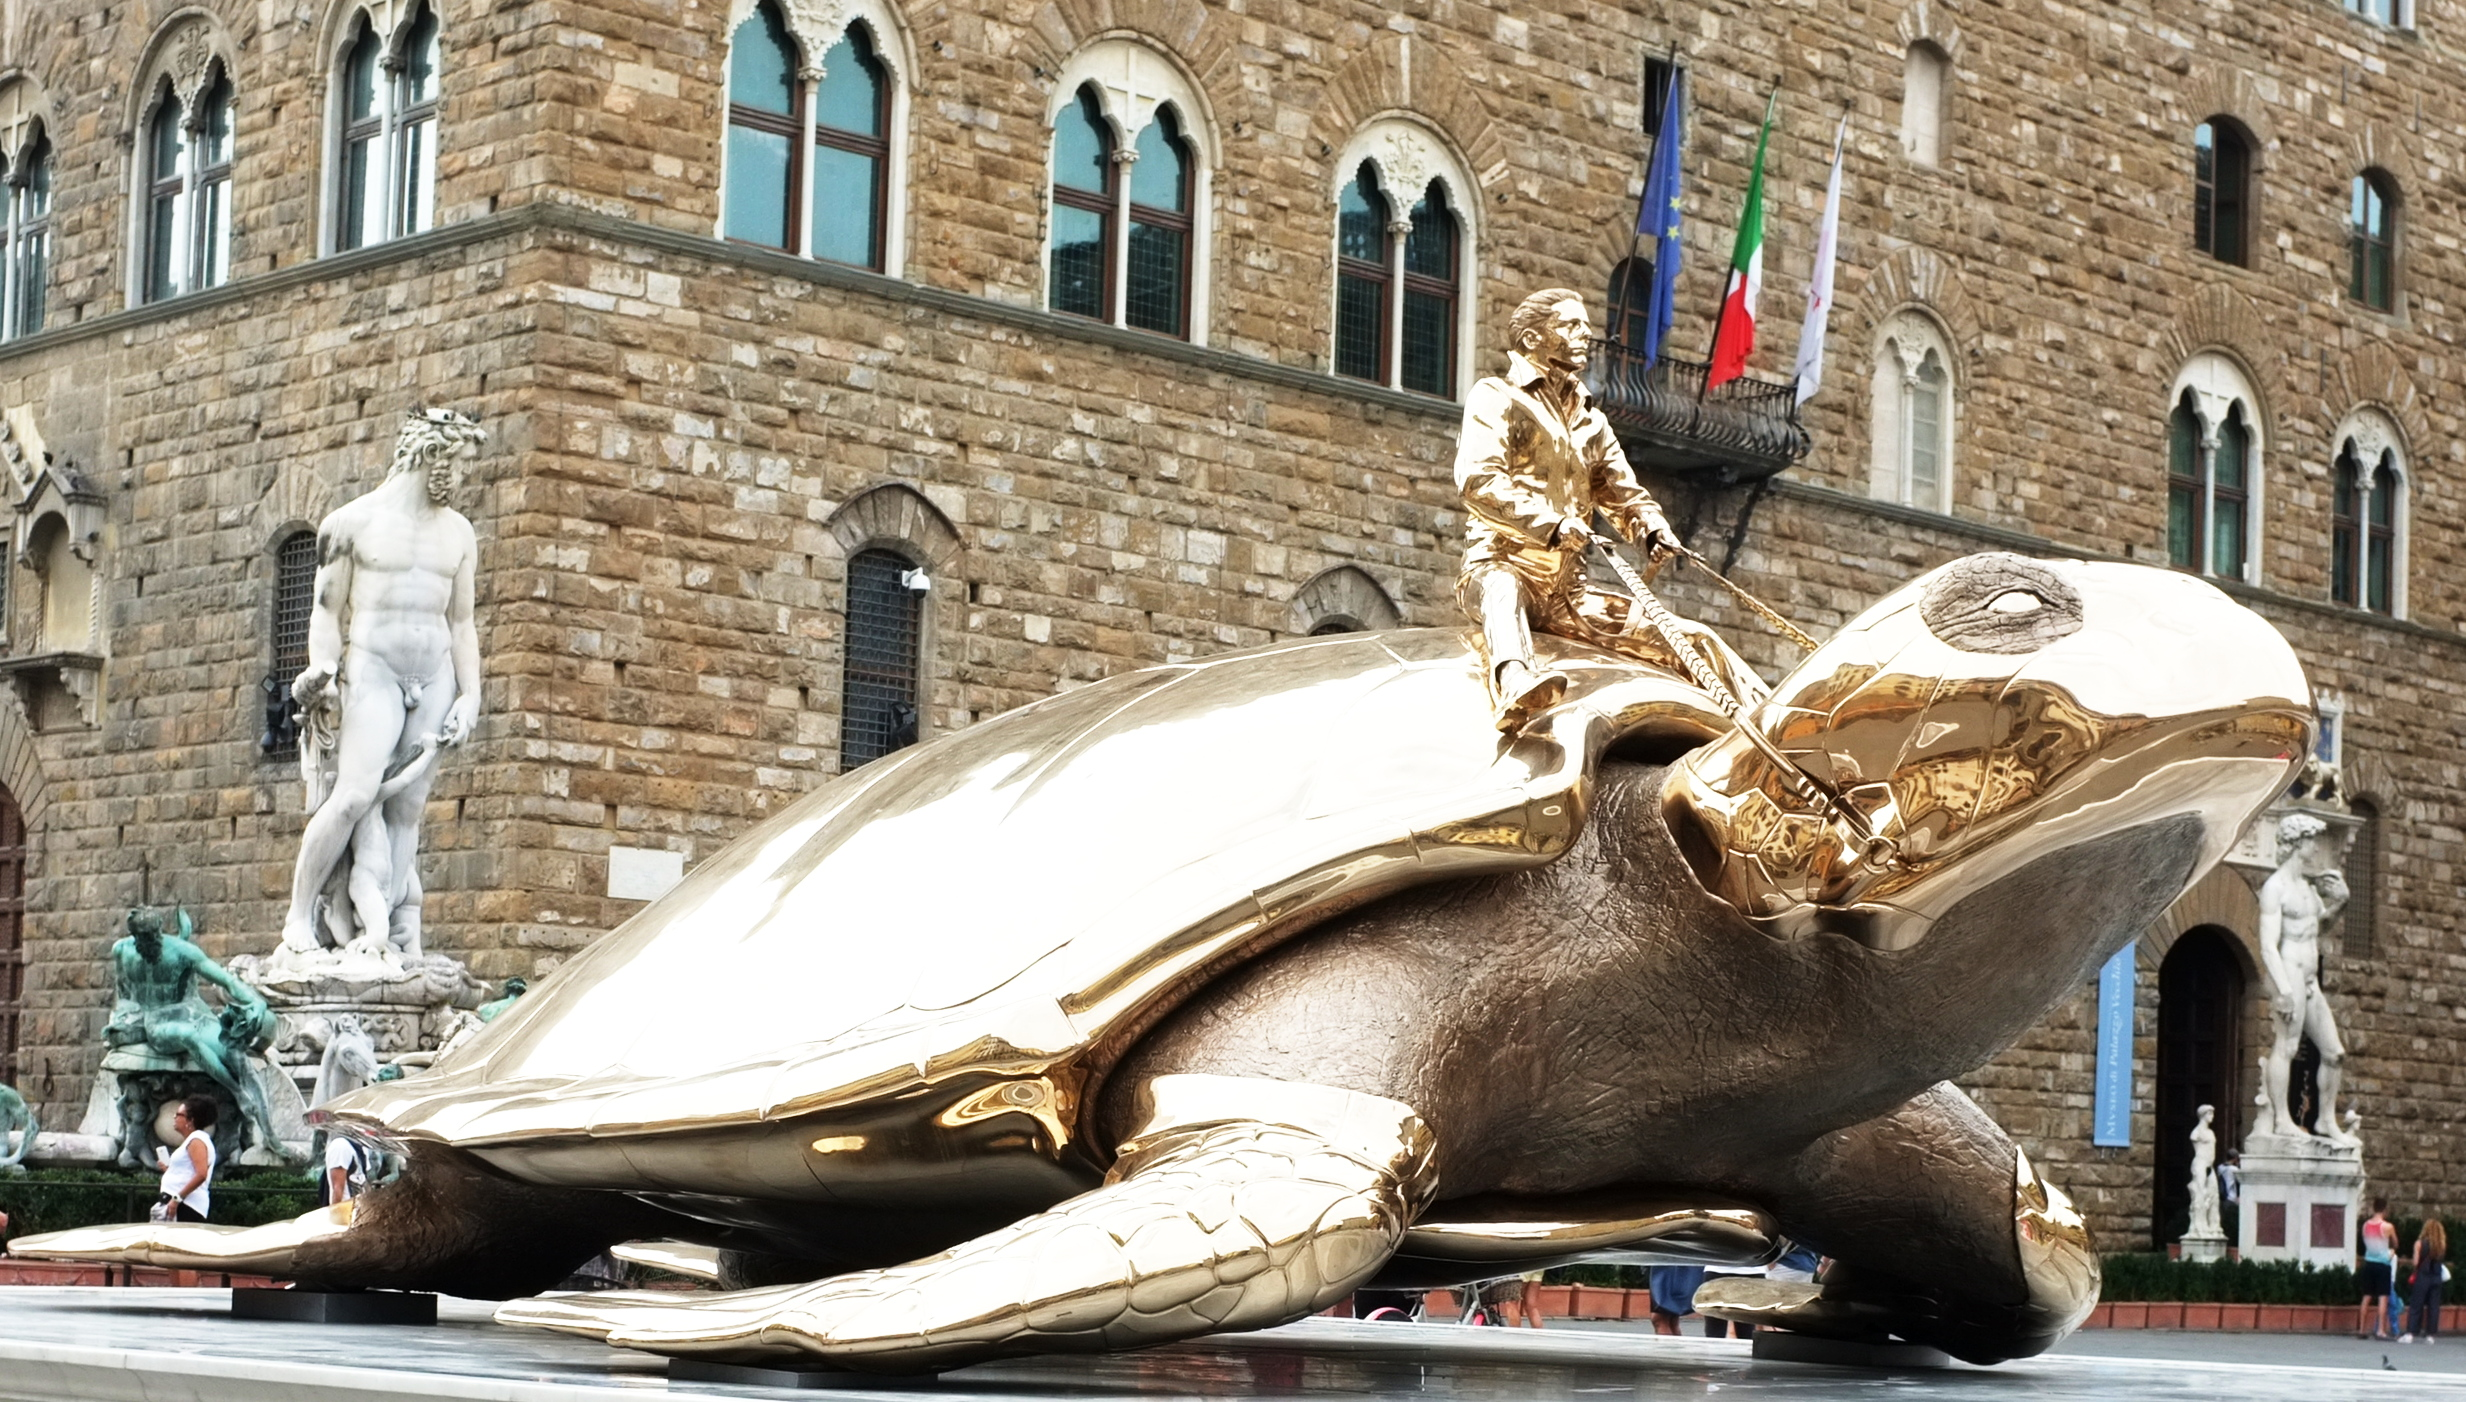
\includegraphics[width=10.0cm]{./images/frontespizio/utopia.jpg}
   \caption{Jan Fabre, "Searching for Utopia", 2003} 
   \label{utopia}


\vfill
{\bfseries \vskip4cm \footnotesize 
Quest'opera è stata rilasciata con licenza 
\\Creative Commons Attribuzione 2.5 Italia. 
\\Per leggere una copia della licenza visita il sito web http://creativecommons.org/licenses/by/2.5/it/ o spedisci una lettera a Creative Commons, PO Box 1866, Mountain View, CA 94042, USA.\\
}    
\vfill

\end{figure}

\end{titlepage}


\tableofcontents
\newpage

\section{Ringraziamenti}

In primo luogo ringrazio tutti gli studenti che si sono impegnati oltre le aspettative nel Laboratorio di Tecnologie Informatiche del Corso di Laurea in Scienze della Formazione Primaria, che si è tenuto nell'anno Accademico 2016/2017. L'esplosione di creatività emersa nei liberi esercizi con Logo è stata di grande aiuto nello sviluppo di questo lavoro. 

Poi ci sono stati alcuni contributi particolari, primo fra tutti quello, notevolissimo, di Marta Veloce, i cui "Esercizi di creatività" hanno ispirato il capitolo \ref{cap:marta}. 

Per la seconda parte del medesimo capitolo sono invece debitore a Alberto Averono, insegnante di informatica in un istituto tecnico, che nell'ambito delle attività svolte nel Corso di Perfezionamento "Le competenze Digitali nella Scuola" (2016/2017) ha suggerito delle interessanti variazioni alla proposta di Marta. Uno splendido invito all'impiego verticale di LibreLogo.

Va ringraziata anche la studentessa, della stessa classe di Maria, Eleonora Aiazzi, con il suo testo "Se incontri un professore che ti tratta come un bambino", dove non ha parlato di coding esplicitamente ma ha colto perfettamente il senso del dispositivo didattico che abbiamo tentato di utilizzare. Feedback come questi sono fondamentali per una proposta didattica del genere e rappresentano un contributo importante nella definizione del taglio di un opera come questa.

Abbiamo quindi Antonella Colombo, insegnante di matematica alla scuola primaria, che ci ha regalato una bellissima documentazione di apprendimento sintonico del cerchio, alla Papert. È da questa bella storia che abbiamo presso le mosse per raggiungere alfine la cometa di Halley, nel capitolo \ref{cap:cerchio}.

Un particolare ringraziamento va anche a Giuseppe Albano, un sicuro e raro riferimento per la competenza pedagogica ma anche tecnica. A lui sono grato per il prezioso confronto che mi consente di recuperare riferimenti che avrei faticato a trovare altrimenti, soprattutto per quanto riguarda una fase che definirei d'oro, nella quale ha visto la luce negli anni '70 - '80 un pensiero tecnico-pedagogico del quale si sono, temo, un po' perse le tracce. Un alleato importante insomma. È grazie Giuseppe che ho potuto inserire in bibliografia il testo di Horacio Reggini, Logo: "ali per la mente"\cite{Reggini}, nel quale ho trovato corrispondenze davvero confortanti con il pensiero che sto cercando di promuovere.

Grazie anche all'amico Piero Salonia che mi ha regalato una meticolosa revisione di bozze.

In ultimo grazie a Antonio Fini, "socio" nella conduzione del Laboratorio di Tecnologie Didattiche nella veste di tutor.

Eh... ma sì, grazie al meraviglioso mondo di Linux, che con i suoi "attrezzi" - scp, ssh, rsync, grep, find, nmap, pdflatex, bibtex e via dicendo - mi dona superpoteri ignoti nel mondo dei touchscreen, consentendomi di volare leggiadramente fra router, PC di ogni tipo, server lontani. La vera Internet, la vera libertà. 

\part{Manuale ragionato di LibreLogo} \label{parte:manuale}

\section{Prefazione}
Questo piccolo manuale nasce per la necessità di fornire supporto di studio e
consultazione nell'insegnamento “Laboratorio di Tecnologie Didattiche” al V
anno del Corso di Laurea Magistrale a ciclo unico “Scienze della Formazione
Primaria” e nell'insegnamento “Laboratorio di Gestione dei Processi Formativi”
al II anno del Corso di Laurea Magistrale “Scienze dell'Educazione degli
Adulti, della Formazione Continua e Scienze Pedagogiche”, presso l'Università
di Firenze, e nell'insegnamento “Informatica” al I anno del Corso di Laurea
Magistrale “Innovazione Educativa e Apprendimento Permanente” presso
l'università telematica Italian University Line. Il manuale guida all'impiego
del linguaggio Logo nella versione LibreLogo implementata all'interno del \textit{word}
\textit{processor} Writer della \textit{suite} di programmi di produttività personale
LibreOffice. LibreLogo è un \textit{plugin} disponibile di \textit{default} in Writer a partire
dalla versione 4.0 di LibreOffice. È stato scritto in linguaggio Python da
László Németh. La documentazione disponibile si trova in http://librelogo.org,
da dove, in particolare, si può scaricare una guida dei comandi di LibreLogo in
italiano \cite{LibreLogo}. Per il resto, sfortunatamente e per quanto è a mia conoscenza sino ad oggi, la documentazione disponibile è tutta in ungherese, principalmente sotto forma di un manuale di esempi scritto dallo stesso László Németh \cite{LibreLogo2} e da un manuale esteso scritto da Lakó Viktória \cite{LibreLogo3}. È a quest'ultimo lavoro che, in una prima fase si è ispirato il presente piccolo manuale, senza tuttavia esserne una traduzione, per vari motivi. In primo luogo io non so l'ungherese e non posso quindi pretendere di poterne fare una vera traduzione e i tempi e le circostanze non mi consentono di avvalermi di un traduttore. Posso tuttavia seguirne le tracce, aiutandomi con i codici (anche se in ungherese quelli si possono imparare), le figure e Google Translate. Del resto, alla fine una traduzione pedissequa non sarebbe nemmeno desiderabile perché viene naturale riformulare il materiale in funzione degli obiettivi specifici e della propria visione della materia. Inoltre, nel corso della traduzione, mi è capitato sempre più spesso di seguire la traccia dei miei pensieri e, alla fine, è stato inevitabile tornare alla fonte primigenia, ovvero al testo con cui Seymour Papert descrisse per la prima volta compiutamente il pensiero che aveva dato origine a Logo, \textit{Mindstorms} \cite{Papert}. È così che ho introdotto la traduzione di due capitoli di \textit{Mindstorms}: il secondo, “\textit{Mathofobia: the Fear of Learning}”, e il terzo, \textit{“Turtle Geometry: A Mathematics Made for Learning”}.

L'immersione profonda nel pensiero di Papert ha poi prodotto un fenomeno interessante. Nei
numerosi passaggi dove Papert insiste sulla necessità di proporre agli studenti nuove idee
matematiche facendo leva sulle conoscenze già possedute (non solo scolastiche) dagli studenti e sul loro coinvolgimento personale, sempre più spesso mi venivano in mente le lezioni di Emma
Castelnuovo, con le quali si impiegano materiali semplici per introdurre tanti concetti matematici. Ad esempio \cite{Castelnuovo}. In questo
libro si riportano alcune lezioni fatte da Emma Castelnuovo presso la Casa-laboratorio di Cenci (Franco Lorenzoni), fra il 2002 e il 2007. La ricerca didattica di Emma Castelnuovo ha riguardato molto l'impiego di materiali semplici per lo studio attivo della matematica.:

\begin{quote}
Ho capito, insomma, che partendo da un materiale semplicissimo (sbarrette, spaghi, elastici ecc.) si potevano costruire i vari capitoli della geometria, motivando i ragazzi a partire da problemi reali. Bastava variare qualche elemento, lasciandone invariati altri, per stimolare delle problematiche anche di alta matematica. Bastava saper guardare attorno a noi perché si aprissero nuove vie del pensiero e si arrivasse, quasi da sé, a formare negli allievi uno spirito matematico.
\end{quote}

Questo pensiero è in accordo completo con quello di Papert. L'unica differenza è costituita dal
contesto nel quale i due autori vanno a ricercare l'interesse e il coinvolgimento degli allievi. Si può dire che la geometria della Tartaruga è un analogo dei materiali fisici usati da Emma Castelnuovo.
Le due visioni e le pratiche che ne scaturiscono non sono affatto in opposizione bensì
complementari. In questa prospettiva, con LOGO si continua e si estende il lavoro
(necessariamente) iniziato con i materiali fisici mantenendo lo stesso identico approccio
pedagogico.

Tutte le figure sono state prodotte con LibreLogo stesso. I codici, adeguatamente commentati, di alcune delle figure sono listati in appendice, come esempio e spunto per ulteriori sviluppi. Nel momento in cui scrivo queste righe ho completato solo il primo capitolo ma trovo utile rendere il lavoro disponibile anche per ricevere eventuali riscontri che potrebbe essere utile per il resto.

\section{Prefazione alla versione 1.0 (settembre 2017)}

L'obiettivo, in questa estate che volge al finire, era quello di iniziare la nuova stagione didattica con tutta la seconda parte completata. Nel frattempo però ho dovuto cambiare completamente il metodo di scrittura, passando, anzi tornando nel mio caso, a \LaTeX, l'unico modo serio di costruire un documento complesso e tipograficamente ineccepibile. E l'unico modo serio per evitare il mal di testa che inevitabilmente coglie chi si azzarda a utilizzare un \textit{word processor} WYSWYG per redigere lavori di una certa dimensione. Questo mi ha obbligato a rimettere mano a tutto il materiale ma ne è valsa la pena. Chi è interessato a approfondire la questione di \LaTeX  può farsi avanti. È un'altra forma di \textit{coding}, se vogliamo, nella stessa logica di HTML. Infatti è un linguaggio di \textit{markup}. non può mancare nel bagaglio di chiunque voglia dedicarsi alle discipline STEM, e forse non solo. 

\section{Prefazione alla versione 1.1 (gennaio 2018)}

Questa versione si differenzia per l'aggiunta della sezione \ref{sez:soluzione-matematica} sulla soluzione matematica del quesito posto da una studentessa, Marta Veloce, intorno al numero di ripetizioni necessarie per la chiusura di cicli di disegno con deviazione totali diverse da 0 o multipli di 360\degree. Marta pose il suo quesito durante la prima edizione del Laboratorio di Tecnologie Didattiche a Scienze della Formazione Primaria il 6 novembre 2016, inviando una decina di pagine di riflessioni in equilibrio fra esplorazione estetica e ragionamento geometrico. Lo scritto si concludeva con la formulazione di una congettura sulla chiusura delle figure geometriche emerse dalla sua esplorazione. Il testo di Marta è riportato nella sezione \ref{sez:esercizi-creativita}

Il mio dovere primario, nel ruolo di professore universitario è quello di rispondere agli studenti. Questo dovere supera quello della ricerca e supera anche la semplice "didattica erogativa", in una scala di valore, perché la domanda difficile di uno studente rappresenta il premio di un percorso dove ricerca e insegnamento hanno innescato una scintilla creativa nella mente di un giovane. Non c'è niente di più alto.

Domande come quella di Marta sono destabilizzanti perché è difficile rispondere. A volte la risposta non c'è. Sono domande vere, domande di ricerca, per tentare di rispondere alle quali occorre onestà intellettuale e umiltà. Discutemmo appronditamente in classe la questione e spiegai subito che la soluzione vera, quella matematica io non l'avevo. Una soluzione matematica è quella che consente di risolvere il quesito in tutte le condizioni possibili. È una soluzione generale. In quella circostanza sviluppai una risposta che consentiva di rispondere al quesito di Marta ma solo nei casi da lei esplorati in una tabella (\ref{tabella-marta}) esposta al termine del suo elaborato. Si trattava cioè di una soluzione euristica, ovvero una soluzione basata su ragionevoli intuizioni ma non ancora sostenuta da un'argomentazione teorica esaustiva. La risposta, ancorché insufficiente, aveva valore didattico perché ci consentiva di mettere a fuoco il significato di verità matematica, tramite il concetto di soluzione euristica. 

Successivamente, durante il corso di perfezionamento “Le competenze digitali nella scuola”, attivato presso il Dipartimento di Scienze della Formazione e Psicologia dell'Università di Firenze nell'anno accademico 2016/2017, sotto la direzione della collega Ranieri, uno dei corsisti, Alberto Averono riprese in mano la questione proponendo una soluzione informatica. L'idea era quella di fornire alla Tartaruga la capacità di riconscere lo stato dal quale era partita in modo da potersi fermare esattamente in quel punto, a partire dal quale avrebbe solo potuto ripetere il percorso fatto. Una soluzione del genere può essere generata per via software, introducendo delle istruzioni che consentano di confrontare lo stato corrente della Tartaruga con quello iniziale. Queste considerazioni hanno consentito di mettere in luce due fatti molto importanti: il concetto di ``stato'' di un sistema, la Tartaruga in questo caso, e la nozione di numero digitale, quale pallida approssimazione dei numeri matematici. Questi fatti sono stati analizzati nella sezione \ref{sez:alternativa-alberto}, In ogni caso, anche se l'approfondimento di Alberto si è rivelato didatticamente assai proficuo, non ci ha fornito la soluzione matematica che desideravamo.

E infine è arrivata anche questa ma è stato necessario approfondire la teoria, cosa che non mi sarei mai aspettato di dover fare in queste circostanze. Ebbene, le questioni affrontate da Marta in sostanza sono quelle che si sono posti Abelson e diSessa\cite{Abelson} nel loro trattato sulla Turtle Geometry. Nella sezione \ref{sez:soluzione-matematica} ho descritto in dettaglio i tratti essenziali della soluzione generale del problema di Marta, fornendo anche il codice per attuarla. La versione 1.1 si distingue dalla 1.0 essenzialmente per questa sezione, a parte altri marginali aggiustamenti.

Un altro aspetto peculiare della versione 1.1 è il fatto che, provvisoriamente, il capitolo \ref{cap:papert2} sia attualmente espunto e disponibile in un file pdf separato e scaricabile da http://iamarf.ch/unifi/Papert-introduce-Logo.pdf. Il motivo sta nel fatto che devo ancora completare il porting verso il sistema di scrittura \LaTeX, di gran lunga più appropriato per la gestione e l'autopubblicazione di questo tipo di testo.

La prossima versione del Piccolo Manuale di Librelogo sarà la 2.0. In questa i capitoli \ref{cap:papert} e \ref{cap:papert2} verranno riuniti e integrati meglio rispetto a alla presente versione. Allo stesso tempo tutto i sorgenti del manuale verranno trasferiti in Github, più adeguato alla gestione di un progetto articolato e complesso.


\chapter{LibreLogo} \label{cap:librelogo}

LibreLogo è l'unione del celebre programma Logo e il \textit{word} \textit{processor} Writer, che è l'equivalente di Word. Word fa parte della ben nota \textit{suite} Microsoft Office mentre Writer fa parte di LibreOffice, che è software libero. Logo è stato creato negli anni 70 da Seymour Papert per facilitare l'insegnamento della matematica mediante il computer. Seymour Papert è un matematico nato in Sudafrica nel 1928., ha studiato matematica a Johannesburg e poi a Cambridge. Ha fatto ricerca in una varietà di luoghi fra cui l'università di Ginevra, fra il 1958 e il 1963. È in questo periodo che ha lavorato con Jean Piaget, diventando uno dei suoi collaboratori preferiti – interessante connubio fra un matematico e un pedagogista. Nel 1963 è stato ricercatore presso il MIT (Massachusetts Institute of Technology) dove, nel 1967, è stato nominato codirettore del celebre MIT Artificial Intelligence Laboratory dal direttore fondatore, Marvin Minsky. Lo stesso laboratorio dove pochi anni dopo avrebbe operato Richard Stallman, ideatore del concetto di software libero e autore dei primi fondamentali componenti software su cui, negli anni '90, si sarebbe basato il software operativo Linux.  Papert è famoso per avere inventato Logo, un linguaggio che consente di creare grafica manovrando il movimento di una “tartaruga” mediante opportuni comandi. Nella prima versione, ideata negli anni '70, la tartaruga era in realtà un robot che disegnava mentre si muoveva.
\begin{figure}
   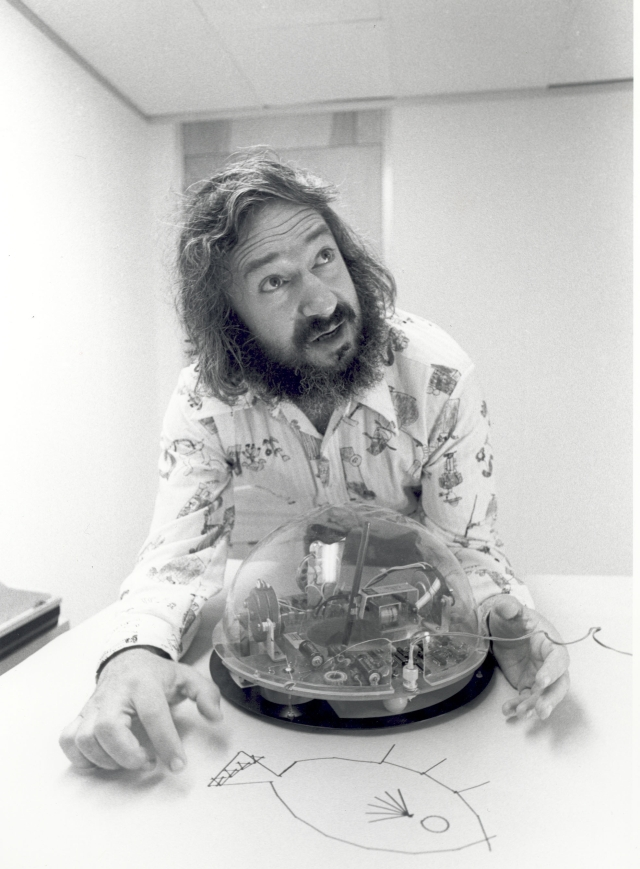
\includegraphics[width=10.0cm]{./images/librelogo/Papert-x640.jpg}
   \caption{Seymour Papert mostra una delle prime versioni di Logo, quando era ancora un vero e proprio robot per disegnare.} 
\label{papert}
\end{figure}
Quando i computer arrivarono nelle case, negli anni '80, Logo divenne un software e come tale è stato descritto da Seymour Papert  in \textit{Mindstorms}. Per capire la valenza pedagogica del pensiero di Papert leggiamo questo brano, tratto proprio da \textit{Mindstorms} (pp. 7-8) \cite{Papert}:

\begin{quote}
Da Piaget prendo il modello del bambino come costruttore delle proprie strutture mentali. I bambini hanno il dono innato di imparare da soli e sono in grado di assumere un'enorme quantità di conoscenza grazie a un processo che io chiamo “apprendimento piagetiano”, o “apprendimento senza insegnamento”. Per esempio, i bambini imparano a parlare, imparano la geometria intuitiva necessaria a muoversi nel loro ambiente, e imparano abbastanza logica e retorica per cavarsela con i genitori – tutto questo senza che venga insegnato loro niente. Ci dobbiamo domandare come mai vi sono cose che si imparano così presto e spontaneamente mentre altre vengono apprese molti anni dopo o non vengono apprese affatto, se non con l'imposizione di un istruzione formale.  Se prendiamo sul serio l'immagine del "bambino costuttore" allora siamo sulla buona strada per trovare una risposta a questa domanda. Tutti i costruttori hanno bisogno di qualche tipo di materiale per costruire qualcosa. Dove il mio pensiero diverge da quello di Piaget è nel ruolo che attribuisco al contesto culturale come fonte di tale materiale. In alcuni casi, il contesto ne fornisce in abbondanza, facilitando così l'apprendimento    costruttivo Piagetiano. Per esempio il fatto che così  tante  cose importanti (coltelli e forchette, madre e padre, scarpe, calze) compaiano usualmente in coppia rappresenta un "materiale" per la costruzione di un senso intuitivo di numero. Ma in molti casi dove Piaget invocherebbe la complessità o la natura formale di un concetto per spiegare la lentezza del suo sviluppo, io trovo che il fattore critico sia piuttosto la carenza dei materiali  che avrebbero reso il concetto semplice e concreto. 
\end{quote}

Negli anni '90 Logo circolava come un programma installabile da un floppy disk. Una volta lanciato produceva uno schermo nero sul quale si potevano scrivere delle istruzioni in sequenza, una dietro l'altra. Le istruzioni rappresentavano i movimenti da impartire alla tartaruga sulla schermo. Poi, con un comando speciale, si poteva “eseguire” la sequenza dei comandi, e così la tartaruga si muoveva tracciando un disegno sullo schermo. Logo ha avuto una grande risonanza come metodo sperimentale per l'insegnamento della matematica e ne sono state derivate una grande varietà di versioni, arrivando fino a generalizzazioni come l'attuale Scratch. Tuttavia non ha avuto una grande diffusione nelle scuole e forse si può dire che ha avuto più successo con gli scolari a cui è stato offerto che con gli insegnanti. Probabilmente era troppo presto. Usare Logo vuol dire scrivere codice, un'attività estranea alla preparazione della maggior parte degli insegnanti, anche di materie scientifiche. Oggi forse è diverso, si parla molto di \textit{coding}, anche se forse non sempre con cognizione di causa. La situazione si è talmente evoluta che \textit{coding} può significare tante cose diverse. Del resto, dagli anni 80 ad oggi la varietà di linguaggi di programmazione si è allargata a dismisura. La cosa più affine a Logo è Scratch, che anzi, deriva proprio da Logo. Mitchel Resnick, leader del progetto Scratch, è stato un allievo di Papert e opera sempre nel Media Laboratory del MIT. Scratch va molto oltre la produzione di grafica e consente di realizzare animazioni e videogiochi, consentendo così anche di sperimentare tecniche di programmazione piuttosto sofisticate. Un altro aspetto innovativo consiste nel fatto di essere strutturato come un servizio web e questo ha consentito di realizzare una grande comunità viva di diffusione e scambio dei programmi. Dal punto di vista operativo Scratch si differenzia da Logo per il fatto di essere un linguaggio visuale. I comandi infatti sono costituiti da blocchi colorati che possono essere incastrati fra loro. Il programma nasce dall'esecuzione di queste sequenze di comandi uniti fra loro, come in un puzzle. È un sistema attraente che si rifa un po' all'idea del Lego, dove le istruzioni da dare al computer vengono incastrate fra loro come mattoncini. Gli incastri garantiscono che le istruzioni vengano combinate solo in modi legittimi, mettendo al riparo dai tipici e frequenti errori ortografici e sintattici in cui incorre chiunque scriva un software nel modo testuale convenzionale. Ne sono emersi tanti di linguaggi di questo tipo, oltre a Scratch, i più noti sono Snap!, Alice, Blockly, Android App Inventor, giusto per menzionarne alcuni. La figura seguente illustra la differenza fra un codice di tipo testuale e uno di tipo visuale. Il codice serve a disegnare un quadrato. A sinistra la versione in LibreLogo e a destra la versione in Snap!. In Scratch questo semplice codice sarebbe identico. Ho utilizzato Snap! Per una mia certa preferenza per questo linguaggio. Snap! rappresenta un potenziamento di Scratch, che lo rendono più assimilabile ad un linguaggio di uso generico, pur mantenendo la forma visuale. Fra queste caratteristiche vi è quella di consentire il salvataggio del codice in un formato standard (XML) leggibile e alterabile con un qualsiasi editore di testo. Per chi è abituato a lavorare con il software questo è un elemento molto importante.Il codice non è, come si suole dire, “ottimale”, in nessun senso. È giusto il modo che utilizza le istruzioni più semplici, le prime che si imparano, in ambedue i linguaggi. L'esempio è pensato solo per confrontare le istruzioni nei due diversi ambienti. 
\begin{figure}
   \centering
   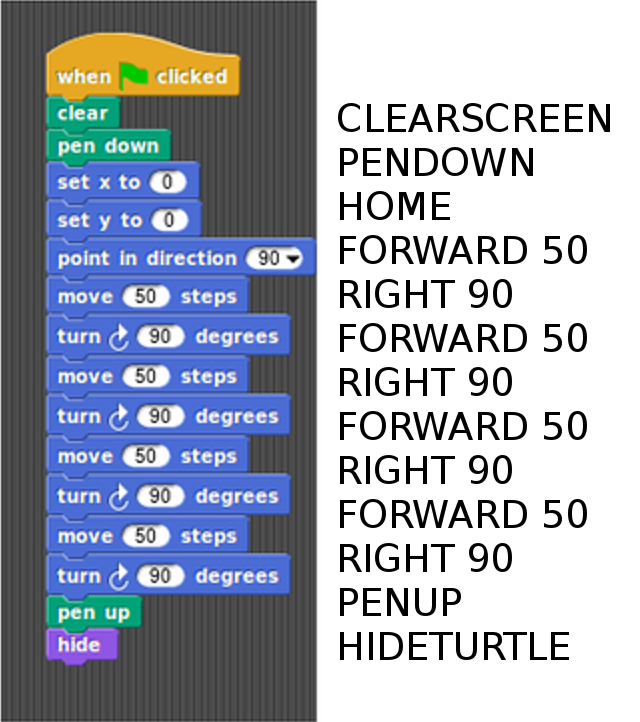
\includegraphics[width=7.5cm]{./images/librelogo/scratch-2.png}
   \label{scratch}
\end{figure}

Una caratteristica particolare di Scratch è quella di avere dato vita ad una vasta comunità di condivisione dei software. Questo è avvenuto grazie al fatto di essere stato concepito come un servizio web, che consente la composizione dei programmi e la possibilità di farli girare ma anche la realizzazione dell'aspetto \textit{social}, destinato alla condivisione e al riuso dei programmi. 
I linguaggi visuali non portano solo vantaggi. Sono (apparentemente) facili, divertenti e colorati, l'efficacia sembrerebbe garantita ma l'evidenza scientifica non è altrettanto chiara. Esistono infatti vari studi che mostrano come i linguaggi visuali non facilitino di fatto l'apprendimento dei linguaggi “veri” \cite{Weintrop}. 

Sembra che siano vantaggiosi per capire i più semplici costrutti della programmazione, questo sì, ma gli studi dove si testano le reali capacità di comprensione di quello che si ottiene con un certo codice non mostrano differenze sostanziali fra linguaggi visuali e testuali \cite{Weintrop2}. 

Particolarmente interessante è la ricerca di Colleen Lewis dove si confrontano i risultati ottenuti con Logo e con Scratch in una classe di bambini fra 10 e 12 anni \cite{Lewis}: se l'apprendimento di alcuni costrutti sembra facilitato da Scratch, non si sono osservate differenze nella percezione degli scolari che, anzi, hanno mostrato un livello di autostima superiore se introdotti alla programmazione con Logo. 

E anche se nelle fasi iniziali i giovani mostrano di gradire gli strumenti di tipo visuale, successivamente, una volta che sono entrati in contatto con la programmazione testuale convenzionale, talvolta sono loro stessi a denunciare i limiti del \textit{coding} visuale, per 1) la minore potenza, ovvero per i limiti imposti alla propria creatività, 2) per la maggiore lentezza nella programmazione quando questa si fa più complessa e 3) perché questi sistemi sono “meno veri”: “se devi fare una cosa vera nessuno ti chiederà mai di codificarla con un software didattico visuale” \cite{Weintrop3}.    

È sulla base di tali considerazioni che abbiamo deciso di approfondire il linguaggio Logo, quale strumento introduttivo alla programmazione. Di versioni di Logo oggi ce ne sono una quantità. Noi qui ci concentriamo su una versione che si trova normalmente nel programma di \textit{word} \textit{processing} Writer, incluso  nella suite per ufficio LibreOffice\footnote{Esiste un altro progetto analogo che si chiama OpenOffice. La domanda su quali siano le differenze rispetto a LibreOffice è molto frequente. Una piccola storia dell'evoluzione di questi due software, che hanno un origine comune, può essere trovata qui (luglio 2016): http://www.navigaweb.net/2014/04/differenze-tra-openoffice-e-libreoffice.html. Allo stato attuale, LibreOffice conviene perché incorpora più funzionalità e viene aggiornato più frequentemente.}, l'analogo del ben noto Microsoft Office. Quest'ultimo è un “prodotto proprietario”, vale a dire che l'azienda che lo produce lo vende ma senza distribuire il codice sorgente in chiaro, secondo il modello industriale convenzionale, con il quale la proprietà intellettuale è tenuta gelosamente segreta.  LibreOffice invece è software libero, e come tale è l'ideale per l'impiego in qualsiasi contesto formativo. In primo luogo perché comporta un messaggio di natura etica. Infatti il software libero è definito da quattro tipi di libertà: 1) libertà di eseguire il programma come si desidera, per qualsiasi scopo ; 2) libertà di studiare come funziona il programma e di modificarlo in modo da adattarlo alle proprie necessità; 3) libertà di ridistribuire copie in modo da aiutare il prossimo; 4) libertà di migliorare il programma e distribuirne pubblicamente i miglioramenti eventualmente apportati, in modo tale che tutta la comunità ne tragga beneficio. Poiché le libertà N. 2 e 4, per potere essere esercitate, richiedono la lettura del codice sorgente del software, va da se che il software libero, per essere tale, deve necessariamente rendere disponibile il codice sorgente. Occorre osservare – su questo punto molti fanno confusione – che il software di tipo \textit{open} \textit{source} non coincide con il software libero (\textit{free} \textit{software}) perché manca la connotazione etica: con il software open source si assume che il codice sorgente sia disponibile in chiaro, ma non si fa menzione delle suddette quattro libertà e, in particolare, delle due specificazioni che connotano la valenza etica del \textit{free} \textit{software}:  “in modo da aiutare il prossimo” nella terza libertà e “in modo tale che tutta la comunità ne tragga beneficio” nella quarta libertà. Il software libero è sviluppato da comunità che al più si aggregano in società non a fini di lucro. L'\textit{open} \textit{source} è sviluppato da attori economici privati che aderiscono al paradigma di sviluppo condiviso perché lo trovano adeguato alle proprie strategie di marketing: vi sono aziende che curano progetti \textit{open\textit{}} source a fianco dei tradizionali prodotti proprietari perché lo trovano conveniente per le proprie strategie di marketing. Le funzionalità di LibreOffice possono essere arricchite da numerosi \textit{plugin}, ovvero componenti che aggiungono le funzionalità più diverse. Ebbene, LibreLogo è uno di questi e, dalla versione 4.0 in poi, il plugin LibreLogo è incluso di \textit{default} \footnote{Di \textit{default} significa che questo è il comportamento normale. Coloro che utilizzano Linux (per Windows o Mac questo problema non c'è) devono prendere nota di quanto segue. Fino alla versione LibreOffice 4 esclusa, installare l'estensione di LibreOffice da http://extensions.libreoffice.org/extension-center/librelogo. Invece dalla versione 4 in poi, installare direttamente il pacchettolibreoffice-librelogo, con il comando \textit{sudo apt-get install libreoffice-librelogo}. Dopodiché occorre fare ripartire LibreOffice, qualora fosse già aperto. Quindi attivare la toolbar in View->Toolbars->Logo. Richiudere e rilanciare
} nel programma. Ma cosa significa usare Logo in un \textit{word} \textit{processor} come Writer, se questo è un normale word processor mentre Logo è un linguaggio per disegnare? Semplice: con il \textit{plugin} LibreLogo si possono produrre immagini che risultano integrate nel documento, come se fossero importate. È un'idea geniale, dovuta a Németh László, che ha riprodotto tutte le funzionalità di Logo all'interno di LibreOffice. In  realtà le ha ulteriormente incrementate, traendo vantaggio dal linguaggio Python, con cui ha scritto il plugin. Usare LibreLogo è semplicissimo: si apre un documento in Writer, si scrive un po' di codice in linguaggio Logo, come fosse un qualsiasi altro testo, e poi si esegue premendo l'apposito tasto nella \textit{toolbar} di LibreLogo; se il codice è corretto, la tartaruga esegue il disegno codificato nel testo in mezzo alla pagina. Successivamente, questo disegno può essere gestito e manipolato come qualsiasi altra grafica di LibreOffice. Quando si lancia LibreOffice, se non si è mai usato LibreLogo, la \textit{toolbar} di LibreLogo non è attiva. Occorre quindi attivarla, con l'appropriato comando di menu: \textbf{View} $\rightarrow$ \textbf{Toolbars} $\rightarrow$ \textbf{Logo}: 

\begin{figure}[h]
   \centering
   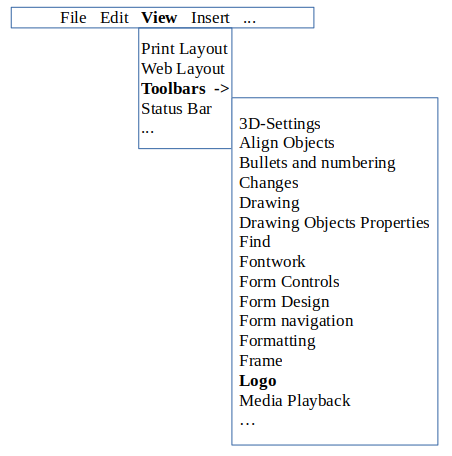
\includegraphics[width=7.5cm]{./images/librelogo/AttivazioneToolbar.png}
   \label{AttivazioneToolbar}
\end{figure}

Fatto questo, occorre chiudere il programma e rilanciarlo per vedere fra le altre \textit{toolbar} anche quella di LibreLogo. Questa appare nel seguente modo: 

\begin{figure}[h]
   \centering
   
\includegraphics[width=7.5cm]{./images/librelogo/LibreLogoToolbar.png}
   \label{LibreLogoToolbar}
\end{figure}

dove le icone hanno i seguenti significati:


\begin{center}
  \begin{tabular}{ c | l | p{5cm} }
    \hline
    
\includegraphics[width=0.75cm]{./images/librelogo/FrecciaSULO.png} & FORWARD 10 & Avanti di 10 punti (vedremo successivamente il significato dei punti) \\ \hline
    
\includegraphics[width=0.75cm]{./images/librelogo/FrecciagiuLO.png} & BACK 10 & Indietro di 10 punti \\ \hline
    
\includegraphics[width=0.75cm]{./images/librelogo/Orario.png} & LEFT 15 & A sinistra di -15 gradi \\ \hline
    
\includegraphics[width=0.75cm]{./images/librelogo/Antiorario.png} & RIGHT 15 & A destra di 15 gradi \\ \hline
    
\includegraphics[width=0.75cm]{./images/librelogo/PlayLO.png} &  & Esegue il programma scritto nel programma. Dalla versione 4.3 in poi, in un documento nuovo appena aperto esegue un programma di esempio. \\ \hline
    
\includegraphics[width=0.75cm]{./images/librelogo/StopLO.png} &  & Ferma il programma che sta girando (se dura troppo a lungo per qualche problema) \\ \hline
    
\includegraphics[width=0.75cm]{./images/librelogo/RewindLO.png} & HOME & Riporta Logo nella condizione iniziale, con la tartaruga al centro che punta in alto. \\ \hline
    
\includegraphics[width=0.75cm]{./images/librelogo/NewpageLO.png} & CLEARSCREEN & Cancella il disegno appena fatto (non il testo presente nel documento) \\ \hline
    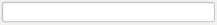
\includegraphics[width=0.75cm]{./images/librelogo/220px-TextLO.png} &  & Consente di scrivere un comando qualsiasi per eseguirlo subito
 \\ \hline
    
\includegraphics[width=0.75cm]{./images/librelogo/MagicwLO.png} &  & Aggiusta tutto il testo del programma rendendolo tutto maiuscolo. Traduce tutti i comandi nella lingua in cui è impostato LibreOffice. Al momento della revisione di queste note (agosto 2017) mi sono accorto che nei sorgenti di LibreLogo è stata impostata la lingua italiana ma il dizionario non è mai stato compilato. Mi riprometto di farlo appena possibile in modo che la modifica venga inserita nella revisione successiva di Libreoffice. \\ \hline
    \hline
  \end{tabular}
\end{center}

\section{La grafica di LibreLogo in Writer}

L'interazione fra LibreLogo e Writer è particolare per quanto riguarda la
grafica. All'inizio può sembrare farraginosa ma in realtà occorre abituarsi e
imparare due o tre regolette. La caratteristica, probabilmente unica, di
LibreLogo è che il risultato ottenuto girando\footnote{In gergo con “girare un
programma” si intende far funzionare un programma – in inglese to \textit{run a
program}. Oggi, con i moderni linguaggi spesso i programmi sono detti
\textit{script}. In generale un programma è un software completo e magari anche
molto complesso. Uno \textit{script} tende a essere un frammento di codice più
piccolo e specifico. Ma sono categorie che si sovrappongono largamente.} uno
script si ritrova sullo stesso supporto dove scriviamo il codice, ovvero un documento di tipo ODT di Writer. Di fatto in questo modo il documento ospita due tipi di informazioni diverse: una lista di istruzioni scritte in forma testuale e un oggetto grafico prodotto facendo funzionare quelle istruzioni. L'oggetto grafico è di tipo “vettoriale”, ovvero è composto da un insieme di oggetti geometrici. Altro sono le immagini tipo \textit{raster}, o \textit{bitmap}, che sono composte da una matrice di pixel\footnote{Un approfondimento della distinzione fra immagini bitmap e vettoriali può essere trovato in http://https://iamarf.org/2014/02/23/elaborazione-di-immagini-tre-fatti-che-fanno-la-differenza-loptis/}. Gli oggetti grafici prodotti da LibreLogo sono del tutto analoghi a quelli che prodotti con il tool di disegno a mano disponibile in Writer, accessibile attraverso l'apposita \textit{toolbar}, alla voce di menu \textbf{View} $\rightarrow$ \textbf{Toolbars} $\rightarrow$ \textbf{Drawing}: : 

\begin{figure}[h]
   \centering
   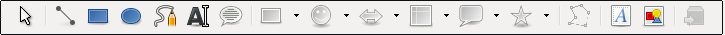
\includegraphics[width=12.0cm]{./images/librelogo/DrawToolbar.png}
   \label{DrawToolbar}
\end{figure}

Come tali, i disegni fatti con LibreLogo possono essere spostati, copiati o salvati come qualsiasi altro oggetto grafico. Una cosa utile da capire è che spesso tali oggetti sono in realtà una composizione di oggetti distinti. In questo manuale ne faremo molti. Per utilizzarli come un unico oggetto occorre usare la funzione di raggruppamento, procedendo così: prima si delimita la regione che comprende gli oggetti da raggruppare, selezionando il \textit{pointer} 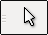
\includegraphics[height=1em]{./images/librelogo/Pointer_LO.png} nella barra di disegno e poi delineando la regione rettangolare desiderata con il mouse e tenendo premuto il tasto sinistro. Attenzione che il cursore del mouse deve avere la forma della freccia e non quella tipica di quando si inserisce il testo, a forma di una I maiuscola, perché con questo si inserisce testo e non grafica. Il fatto che sia attivo il cursore grafico (e non testuale) si capisce anche dal fatto che contestualmente si attiva un'altra toolbar, che serve al controllo della grafica:

\begin{figure}[h]
   \centering
   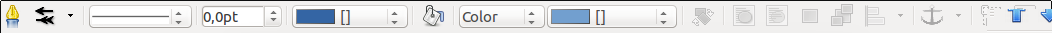
\includegraphics[width=12.0cm]{./images/librelogo/DrawToolbar2.png}
   \label{DrawToolbar2}
\end{figure}

Quando si seleziona la regione che contiene gli oggetti grafici, in questa barra si attivano alcune icone, fra cui quella della funzione raggruppamento: 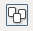
\includegraphics[height=1em]{./images/librelogo/RaggruppamentoLO.png}. Premendo questa tutti gli oggetti grafici compresi nella regione selezionata vengono raggruppati in un unico oggetto grafico che può essere copiato altrove o salvato. 

Un altro accorgimento utile è quello di “ancorare” appropriatamente la grafica al documento, laddove la dobbiamo usare. Sempre nella solita barra per la grafica, il tasto che consente di determinare l'ancoraggio è questa: 
\includegraphics[height=1em]{./images/librelogo/AncoraLO.png}. Cliccando sulla freccetta a sinistra dell'ancora si possono selezionare quattro tipi di ancoraggio: 1) “alla pagina”, 2) “al paragrafo”, 3) “al carattere” e 4) “come carattere”. Nel primo caso la grafica è associata alla pagina e non si muove da questa, nel secondo ad un paragrafo, nel terzo ad un carattere e nel quarto si comporta come se fosse un carattere. Quale sia l'ancoraggio più opportuno è una cosa che si impara con l'esperienza. La maggior parte delle grafiche in questo manuale sono state ancorate “al paragrafo”, eccetto che per le piccole immagini che stanno in linea con il testo, come l'ancora precedente, queste sono ancorate “come carattere”. 

Queste cose appena dette riguardano la gestione della grafica in Writer in generale. Usando LibreLogo, l'unica differenza è che la grafica viene prodotta attraverso le istruzioni che mettiamo nel codice. LibreLogo piazza la grafica nel mezzo della prima pagina del documento, anche se il testo del codice si dilunga nelle pagine successive. Può succedere così che la grafica si sovrapponga al testo del codice medesimo. Di primo acchito sembra che il comportamento sia farraginoso se non errato. Niente di tutto questo. La grafica è prodotta per essere usata da qualche parte. Si tratta semplicemente di selezionarla, con gli accorgimenti appena descritti e portata altrove, in una pagina pulita semplicemente per vederla con chiarezza, oppure in qualche altro documento dove questa debba essere integrata.



















%\chapter{La genesi} \label{cap:papert}

\section{La paura della matematica}

Perché la motivazione fondamentale della genesi di Logo sta tutta nella questione, tutt'ora irrisolta, dell'insegnamento della matematica. Il linguaggio Logo è stato ideato da Papert proprio per cercare di risolvere questo annoso problema per il quale aveva coniato anche un preciso nome, \textit{Mathofobia}, per descrivere la diffusa antipatia verso questa materia. L'interesse di Papert per la questione ha accompagnato tutta la sua vita lavorativa, che si è distesa nella seconda metà del 900. Il suo contributo è stato eccezionale, sia sotto il profilo dell'elaborazione teorica dal punto di vista pedagogico, che della creatività che lo ha condotto a concepire appositamente un linguaggio per avvicinare i ragazzi alla matematica. La profonda competenza, sia nelle questioni matematico-informatiche che in quelle pedagogiche, rende la sua opera unica e spiega la rara capacità di proporre soluzioni concrete. 

La sensazione è che non molto sia cambiato, dagli anni '80 ad ora, almeno in media\footnote{Affermazione che nasconde un mondo di perplessità. Cosa è cambiato? Forse proprio ciò che una “media” non esprime. La scuola cui si riferiva Papert è probabilmente più affine a quella che ha frequentato il sottoscritto (I elementare nel 1960). Allora probabilmente il panorama era più uniforme. “La lo picchi se non capisce perché gliè zuccone!” raccomandò la mamma di un mio compagno di classe alla maestra. I genitori erano alleati di quel sistema scolastico, in una visione formativa che poteva essere coercitiva e punitiva, ma che attraversava tutti i generi di scuole e tutti gli strati sociali. Non c'erano “genitori coach” o “genitori sindacalisti”. Nelle famiglie si lavorava duramente, nelle scuole si faticava. Non c'era ancora il “tempo libero”. La scuola era più brutale, forse iniqua, la pedagogia semplice, ma il panorama era più nitido. Almeno nella provincia rurale degli anni '60 in cui ho vissuto. Ora domina la complessità. Le categorie si intersecano. I dibattiti esplodono, amplificati dai media, a livello microscopico (gruppi di genitori in Wathsapp o Facebook) e a livello macroscopico (stampa, televisione ecc.). Le esperienze personali sono schizofreniche: i miei contatti con il mondo dell'insegnamento rappresentano un quadro affascinante di impegno, studio e sperimentazione; ma le storie private e le narrazioni dei conoscenti sono popolate di pratiche didattiche obsolete e superficiali. La variabilità è allucinante. Dove sta la media? Francamente non sono in grado di valutarlo ma la dispersione è sicuramente molto più ampia di un tempo. A complicare il quadro ci sono le indagini internazionali, paludate di rigore scientifico ma che poi si possono rivelare speratamente fatue. Per alcuni anni è brillata la stella polare della Finlandia nel cielo delle valutazioni PISA dell'OCSE, in particolare per la matematica. Poi emergono una serie di denunce di accademici finlandesi che documentano un crollo delle competenze matematiche: sembra che gli studenti finlandesi siano diventati bravi nei test matematici PISA ma che siano peggiorati in matematica! Leggendo il post di Giorgio Israel “Il bluff della matematica finlandese” (http://gisrael.blogspot.it/2011/05/il-bluff-della-matematica-finlandese.html), che riassume tali denunce, si scopre che i modelli di apprendimento sono banalmente utilitaristici e anche ben lontani dalle idee di Papert che riportiamo qui. Dove sarà la verità? Insomma la confusione regna sovrana e viene seriamente da domandarsi se non ci si debba rassegnare a considerarla inevitabile normalità.}; che la motivazione iniziale, centrata su una seria e difficile rivisitazione del modo di introdurre i giovani alla matematica, sia finita diluita oggi nel calderone del “coding”, nella forma di una sorta di paese dei balocchi, superficialmente entusiasmante per taluni, oggetto di derisione per altri; che il messaggio di Papert, per certi versi estremo e provocatorio, senz'altro da decodificare rispetto ad un'epoca diversa, venga frainteso; che il tutto sia vanificato in sostanza dal fallimento di Logo, rimasto confinato in una minoranza di circoli sperimentali, senza avere rivoluzionato nulla, contrariamente a quelle che sembravano le legittime aspettative di Papert; che invocare la magia della matematica per introdurre i giovani in un dominio comunemente considerato “freddo”, sia un sogno che alla fin fine può concepire solo un matematico, magari un po' idealista, e quindi che solo un'arida via può svelare quella magia, e solo ai pochi in grado di percorrerla, per un motivo o per un altro, e che non possa essere infine altro che così – una cosa che io non voglio pensare ma la paura che sia un po' vera m'è venuta rileggendo \textit{Mindstorms}.

Logo fallito abbiamo detto. Ha fallito nelle intenzioni iniziali di Papert. Non è diffuso nelle scuole e non è adottato come un modo standard per sostenere l'apprendimento della matematica e delle scienze. Ma non ha fallito nel senso di non aver lasciato traccia, al contrario. Ci sono molte versioni del logo in tutto il mondo, alcune delle quali sono diventate importanti strumenti di indagine educativa, ad esempio nel campo della simulazione di sistemi biologici complessi. Ed è sempre da Logo che ha preso spunto il vasto mondo dei linguaggi visivi a blocchi, primo fra tutti Scratch. Logo e Scratch non sono in opposizione. In un certo senso, Scratch deriva da Logo e "contiene" molte delle sue funzionalità. Molte delle cose che puoi fare in Logo possono essere fatte anche in Scratch. Ma Scratch è molto più orientato alla costruzione "del tuo videogioco" o allo storytelling. Il problema, tuttavia, è che questa gamma più ampia di possibilità, in un contesto scolastico caratterizzato da un basso livello di istruzione tecnologica, ha finito per disperdere le intenzioni educative originali di Logo. Una delle intenzioni di questo manuale è quella di recuperare l'originale "sapore matematico" della pratica del \textit{coding} a scuola. Nella prossima sezione commentiamo quella che Papert ha chiamato \textit{mathophobia}, una sorta di malattia che Logo era destinato a combattere. 

\section{\textit{\textit{Mathophobia}: The Fear for Learning}}

Seymour Papert ha scelto di intitolare il secondo capitolo di Mindstorms "Mathophobia: The Fear for Learning". Il suo punto di partenza è la divisione schizofrenica tra scienze umane e scientifiche, una divisione che è profondamente radicata nel linguaggio, nella visione del mondo, nell'organizzazione sociale e nel sistema educativo. Una divisione che negli ultimi 30-40 anni di deriva neoliberista, si è ulteriormente ampliata. Ad esempio, nelle università, a partire dagli anni '80, gli accademici si battono per ottenere i finanziamenti necessari per le loro ricerche. Purtroppo, l'altra faccia della medaglia è che quasi nessuno si preoccupa di insegnare, o molto poco. La carriera di un professore non dipende dalla qualità del suo insegnamento, ma quasi solo dalla quantità della sua produzione scientifica. Le conseguenze sono pessime. Gli accademici tendono a trasformarsi in manager quando fanno ricerca e in funzionari pubblici quando insegnano: imprenditori dinamici da un lato e (forti) conservatori dall'altro. In questo modo, anche nelle scienze umane si assiste a una deriva tecnica del ruolo accademico. La missione dell'insegnamento, che in un certo senso è il "lato umanistico" del lavoro, si riduce a una sorta di Cenerentola. Così, la dicotomizzazione tra scientifico e umanistico è ancora più forte e sbilanciata.

La questione non è quella di un equilibrio adeguato, bensì di spezzare la linea di demarcazione tra le due culture. Papert guardò il computer come una forza per attenuare la distinzione. La pratica del \textit{coding} è stata pensata come un modo per introdurre una matematica più umanistica e per sfruttare elementi di pensiero scientifico nelle scienze umane. È in questo contesto che Papert ha parlato di una \textit{Mathland}, dove la matematica costituirebbe un vocabolario naturale, con l'idea che potremmo cambiare non solo il modo in cui insegniamo la matematica, ma anche il modo in cui la nostra cultura concepisce la conoscenza e l'apprendimento.

Papert sostiene che le sue argomentazioni non si limitano all'apprendimento della matematica, ma riguardano l'atteggiamento nei confronti dell'apprendimento in generale. La parola \textit{matofobia} suggerisce due associazioni. Uno è il diffuso disprezzo della matematica. L'altro deriva dal gambo "matematica", che in greco antico significa apprendimento in senso generale.

%%%%%%%%%%%%%%%%%%%%%%%%%%%%%%%%%%%%%%%%%%%%

Platone sulla sua porta aveva scritto: “Che entrino solo i geometri”. I tempi sono cambiati. La maggior parte di coloro che cercano di entrare nel mondo intellettuale di Platone non conoscono la matematica né percepiscono la minima contraddizione con la sua prescrizione. La schizofrenica suddivisione che la nostra cultura traccia fra le discipline umanistiche e quelle scientifiche supporta il loro senso di sicurezza. Platone era un filosofo, e la filosofia è una materia umanistica tanto sicuramente quanto la matematica una scientifica.

Questa grande divisione è radicata nel nostro linguaggio, nella nostra visione del mondo, nell'organizzazione sociale, nel sistema educativo e, più recentemente, anche nelle teorie neurofisiologiche. È una divisione che si auto-perpetua: più la cultura è divisa, più ciascuna parte rinforza la separazione nella propria crescita.

Ho già suggerito come il computer possa costituire una forza che serva ad abbattere la divisione fra le “due culture”. So che l'umanista può ritenere discutibile che una tecnologia possa influenzare la propria opinione su quale tipo di conoscenza sia rilevante nell'insegnamento. Non meno minacciosa appare allo scienziato la diluizione del rigore causata dall'invasione di pensiero umanistico “annacquato”. Ciò nonostante io penso che con la tecnologia si possano gettare i semi di un'epistemologia culturale meno dissociata. 

La condizione della matematica nella cultura contemporanea presenta i sintomi più acuti di tale dissociazione. L'emergenza di una matematica “umanistica”, che non sia percepita in maniera separata dallo studio dell'uomo e delle discipline umanistiche, potrebbe essere il segno di un mutamento di prospettiva. In questo libro io cercherò di mostrare come un computer possa essere utilizzato per condurre i bambini in una relazione più umanistica e anche più umana con la matematica. Per fare questo dovrò andare oltre la matematica. Dovrò sviluppare una nuova prospettiva del processo di apprendimento medesimo. 

Non è raro che adulti intelligenti si riducano ad essere osservatori passivi della propria incompetenza in tutto ciò che non sia la matematica più rudimentale. E possono subire le conseguenze di una simile paralisi intellettuale anche nella ricerca di un lavoro. Ma le conseguenze secondarie, indirette, sono ancora più gravi. Una delle lezioni principali imparate dalla maggior parte delle persone nelle ore di matematica è una consapevolezza delle proprie rigide limitazioni. Costoro si formano un'idea balcanizzata della conoscenza umana che finiscono col percepire come un collage di territori separati da ferree cortine impenetrabili. Io non metto in discussione la sovranità dei territori intellettuali ma le restrizioni imposte alla libera circolazione fra questi. Non voglio ridurre la matematica alla letteratura o la letteratura alla matematica. Ma voglio argomentare come le rispettive mentalità non siano così separate come viene generalmente supposto. E per fare questo, mi servo di un'immagine, ovvero di una \textit{Mathland}  – dove la matematica sia un vocabolario naturale – al fine di sviluppare l'idea che con la presenza del computer le culture umanistica e matematico/scientifico possano essere riunite. In questo libro, \textit{Mathland} rappresenta il primo passo di un discorso più ampio su come la tecnologia possa cambiare non solo il modo con cui insegniamo la matematica ai bambini, ma anche, in maniera più fondamentale, il modo nel quale la nostra cultura nel suo complesso concepisce la conoscenza e l'apprendimento.

Per me la parola “mathophobia” presenta due associazioni. Una di queste è il diffuso timore per la matematica, che spesso presenta i connotati di una vera fobia. L'altra attiene al significato della radice “math”, che in greco significa “apprendimento”, nel suo senso più generale\footnote{Il significato generale è presente nella parola “\textit{polymath}”, che denota una persona dai saperi multipli. Una parola meno nota con la stessa radice, che userò nei capitoli successivi, è “matetico”: che concerne l'apprendimento.}.  Nella nostra cultura, la paura di imparare non è meno endemica (sebbene molto spesso travestita) della paura della matematica. I bambini all'inizio della propria vita sono avidi di apprendere. Poi sono costretti a imparare ad avere problemi con l'apprendimento in generale con la matematica in particolare. In ambedue i sensi della radice “math” si verifica uno spostamento da matefilia a matofobia. Andremo a vedere le cause di tale spostamento e vedremo qualche idea su come si possa usare il computer per contrastarlo. Iniziamo con qualche riflessione su come apprendano i bambini.

La facilità di apprendimento dei bambini sembra così ovvia che ai più sembra non valga nemmeno la pena di documentarla. Un campo nel quale la capacità di apprendimento è particolarmente chiara è quello dell'apprendimento verbale di nuovi vocaboli. All'età di due anni sono pochi i bambini che conoscono più di qualche centinaio di parole. Ma già quando entrano nella prima classe primaria, quattro anni dopo, conoscono migliaia di parole. È evidente che sono in grado apprendere ogni giorno varie parole nuove. 

Anche se “vediamo” che i bambini imparano le parole, non è altrettanto facile vedere che stanno imparando matematica con la stessa velocità, o anche maggiore. Ma questo è esattamente ciò che ha mostrato Piaget, con lo studio di una vita intorno alla genesi della conoscenza nei bambini. Una delle conseguenze più sottili delle sue scoperte è la rivelazione che gli adulti non riescono ad apprezzare la natura e l'estensione di ciò che i bambini apprendono, perché il fatto che diamo per scontate varie strutture della conoscenza nasconde una buona parte di quell'apprendimento. Questo è evidente in quelle che sono note come le “conservazioni” piagetiane.

\begin{figure}
   \centering
   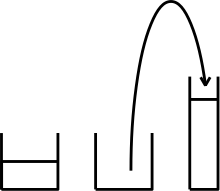
\includegraphics[width=7.5cm]{./images/papert-1/220px-Fig-2-mindstorms.png}
   \label{Papert}
\end{figure}

Per un adulto è ovvio che versando liquido da un bicchiere ad un altro il volume del liquido non cambia (a meno di piccoli effetti, come gocce versate fuori o lasciate nel bicchiere precedente). La conservazione del volume è così ovvia che sembra non sia venuto in mente a nessuno prima di Piaget che ai bambini di quattro anni potrebbe apparire diversamente. Occorre una sostanziale crescita intellettuale prima che i bambini sviluppino una visione “conservazionista” del mondo. La conservazione del volume è solo una delle tante conservazioni che devono imparare.  Un'altra è la conservazione dei numeri. Anche in questo caso, gli adulti faticano a rendersi conto che un bambino   deve imparare il fatto che contando una collezione di oggetti in ordine diverso il risultato sia lo stesso. Per gli adulti l'operazione di contare significa semplicemente determinare quanti oggetti “ci sono”. Il risultato dell'operazione è un “fatto oggettivo” indipendente dall'atto di contare. Ma la separazione del numero dal conteggio (del prodotto dal processo) poggia su presupposti epistemologici che sono non solo ignoti al bambino preconservazionista, ma anche estranei alla loro visione del mondo. Tali conservazioni rappresentano solo una parte della vasta struttura di conoscenza matematica nascosta che i bambini imparano da soli. Nella geometria intuitiva del bambino di quattro o cinque anni, la linea retta non è necessariamente la distanza più breve fra due punti, e che camminare lentamente fra due punti non richiede necessariamente più tempo che camminare velocemente. Anche in questo caso, non è che manchi semplicemente un elemento di conoscenza, bensì il presupposto che sostiene l'idea “del più breve” quale proprietà di un percorso piuttosto che dell'azione di percorrerlo. 

Nessuno di questi casi deve essere interpretato come una carenza di conoscenza da parte del bambino. Piaget ha mostrato come i bambini piccoli abbiano teorie del mondo che, nei propri termini, sono perfettamente coerenti. Queste teorie sviluppate spontaneamente da tutti i bambini, hanno componenti ben sviluppati che non sono meno “matematici”, sebbene esprimano una matematica diversa, rispetto a quella accettata dalla nostra cultura (adulta). Il processo di apprendimento nascosto ha due fasi: già in età prescolare ogni bambino sviluppa teorizzazioni proprie del mondo per poi spostarsi verso visioni caratteristiche dell'età adulta. E questo accade attraverso quello che ho chiamato apprendimento piagetiano, un processo con caratteristiche che la scuola dovrebbe invidiare: funziona (accade in tutti i bambini), è economico (non richiede maestri ne curricula), e è “umano” (i bambini lo attuano con spirito apparentemente disinteressato senza bisogno di riconoscimenti o punizioni esplicite imposti dall'esterno).  

La misura in cui nella nostra società gli adulti hanno perso l'atteggiamento positivo dei bambini nei confronti dell'apprendimento varia da individuo a individuo. Una quota sconosciuta ma certamente significativa della popolazione ha completamente rinunciato a imparare. Queste persone raramente, se non mai, si cimentano nell'apprendimento e non si sentono né competenti né capaci di trarne giovamento. Il costo personale e sociale è enorme: la matofobia può limitare la vita delle persone, culturalmente e materialmente. Un numero ancora maggiore di persone non ha rinunciato completamente ma soffre di pesanti limitazioni a causa di pregiudizi negativi profondamente radicati sulle proprie capacità. La deficienza diventa identità: “Io non posso imparare il francese, non ho orecchio per le lingue;” “Non potrei mai fare affari, non ho la testa per i numeri.” “Non posso imparare lo sci parallelo, non sono mai stato coordinato.” Queste credenze sono spesso manifestate ripetutamente, in modo rituale, come superstizioni. E, come le superstizioni, creano un mondo di tabù; in questo caso il tabù dell'apprendimento. In questo capitolo e nel capitolo 3, discuteremo su degli esperimenti che dimostrano come queste immagini di se spesso corrispondano a una realtà molto limitata – usualmente la “realtà scolastica” di una persona. In un contesto formativo, con un adeguato supporto emozionale e intellettuale, lo “scoordinato” può imparare esercizi circensi come la giocoleria e coloro che “non hanno la testa per i numeri” possono scoprire che non solo sono in grado di capire la matematica ma vi si possono anche appassionare.

Sebbene tali opinioni negative su di se possano essere superate, di fatto sono estremamente tenaci e tendono ad autoconfermarsi. Se uno crede abbastanza fermamente di non poter fare matematica, avrà quasi sicuramente successo nell'impedirsi di fare qualsiasi cosa che gli paia attinente alla matematica. La conseguenza di tale autosabotaggio è il fallimento personale, e ogni fallimento rinforza l'assunto di base. Ancora più insidiosi sono i pregiudizi che appartengono non solo agli individui ma a un'intera cultura.

I nostri figli crescono in una cultura permeata dall'idea che ci siano “persone brillanti” e “persone stupide”. La costruzione sociale di un individuo è costituita da un fascio di attitudini. Ci sono persone “buone per la matematica”  e persone “negate per la matematica”. Tutto è aggiustato in maniera da attribuire i primi insuccessi o esperienze negative dei bambini a loro proprie disabilità. Di conseguenza, i bambini interpretano i fallimenti come sentenze di appartenenza al gruppo delle “persone stupide” o, più spesso, al gruppo delle persone “inadatte per l'attività x” (dove, come abbiamo osservato, spesso x si identifica con la matematica). In un contesto del genere i bambini declinano la propria personalità nei termini delle loro limitazioni, che verranno confermate e consolidate nel corso degli anni. Solo raramente accade che un evento eccezionale induca qualcuno a riorganizzare la propria immagine intellettuale in modo da aprire nuove prospettive su ciò che può apprendere.

Non è facile rimuovere questi pregiudizi sulla natura delle capacità umane. I pregiudizi popolari sono sempre difficili da sradicare. Ma qui le difficoltà sono sostenute da vari altri fattori. In primo luogo, le teorie comuni sulle attitudini umane sembrano essere sostenute da teorie “scientifiche”. Dopotutto, la psicologia si avvale molto di misure attitudinali. Proviamo a mettere in discussione la significatività di ciò che viene misurato mediante l'esperimento mentale di immaginare una \textit{Mathland}. 

Sebbene l'esperimento mentale lasci aperta la questione di come realizzarla una \textit{Mathland}, questo è tuttavia completamente rigoroso nel dimostrare che i pregiudizi comuni sulle capacità matematiche non sono sostenuti da evidenze palesi. Ma siccome i lettori più matofobici potrebbero avere problemi a fare l'esperimento per conto loro, lo riformulo in un altro modo. Immaginiamo di far disegnare ai bambini per un'ora al giorno passi di danza sulla carta e di far sostenere loro un esame su tali “questioni di danza” prima di lasciarli ballare veramente. Non dovremmo in tal caso aspettarci un mondo pieno di “danzofobi”? E non concluderemmo che coloro che ce la fanno a raggiungere la sala da ballo sono i più dotati per la danza? Io credo che sia altrettanto ingiustificato trarre conclusioni  sulle doti matematiche in base allo scarso entusiasmo dei bambini per passare centinaia di ore a fare somme.

Uno può sperare che passando dalle storie ai metodi più rigorosi della psicologia potremmo ottenere dati più consistenti sulle potenzialità degli individui in termini di competenze raggiungibili. Ma non è così: il paradigma corrente nella psicologia della formazione è focalizzato su come i bambini imparano o (più frequentemente) non imparano la matematica nella “anti-\textit{Mathland}” in cui viviamo. Un indirizzo che può essere descritto da questa storia:

\begin{quote}
Immaginiamo una persona del diciannovesimo secolo che volesse migliorare i sistemi di trasporto. Essa sarebbe stata probabilmente persuasa del fatto che la strada per escogitare nuovi metodi passi dalla conoscenza profonda dei metodi esistenti. Sarebbe così partita con uno studio accurato delle differenze fra i vari tipi di carri trainati da cavalli. Avrebbe quindi documentato accuratamente la dipendenza delle velocità ottenibili in funzione della forma e dei materiali degli assi, dei perni e delle finiture.
\end{quote}

Retrospettivamente sappiamo che la strada dell'evoluzione dei mezzi di trasporto è stata completamente diversa. Le invenzioni dell'automobile e dell'aeroplano non hanno preso le mosse dallo studio dettagliato su come i mezzi preesistenti, ovvero i carri trainati da animali, funzionassero o meno.  Ecco, questo è il  modello della ricerca attuale sulle questioni di formazione. I paradigmi usuali per tale tipo di ricerca pongono al centro degli  studi  la classe scolastica. Ci sono molti studi sullo scarso valore dell'insegnamento che viene impartito dalla scuola nella matematica e nelle scienze. È tuttavia diffusa l'idea che un “buon” approccio pedagogico debba basarsi su questi metodi, in realtà poveri di pensiero. Si può simpatizzare con le buone intenzioni, tuttavia penso che tali strategie riflettano il desiderio di mantenere il sistema tradizionale. Come dire di ritenere che convenga migliorare gli assi dei carri a trazione animale. Invece la questione importante sarebbe quella di inventare l'“automobile della formazione”. Questo problema (tema centrale di questo libro) non viene di fatto affrontato e, di conseguenza, ci sembra che le basi scientifiche che sostengono le assunzioni comuni sulle attitudini siano piuttosto labili. Assunzioni che tuttavia sono istituzionalizzate nelle scuole, nei sistemi di valutazione e di ammissione nelle università, al punto che la loro radicazione sociale è tanto forte quanto deboli sono i presupposti scientifici. 

Dalla scuola dell'infanzia in poi, i bambini sono sottoposti a prove basate su capacità verbali e quantitative concepite come entità “vere” e separabili. I risultati di tali test si trasformano in un corredo di attitudini che determinano la costruzione sociale del bambino. Una volta che Johnny e il suo maestro condividono la percezione che Johnny è una persona dotata per l'arte ma non per la matematica, tale percezione tende inevitabilmente a rinforzarsi con il tempo. Questo è un fatto largamente accettato nella psicologia della formazione. Ma il modo in cui la scuola forma le attitudini presenta aspetti più profondi. Consideriamo il caso di un bambino  che ho seguito durante i suoi ottavo e nono anni di età. Jim era un bambino molto loquace ma matofobico appartenente ad una famiglia di professionisti. La sua passione per le parole e il piacere di parlare si erano manifestate molto prima di andare a scuola. La matofobia era invece comparsa a scuola. La mia teoria è che essa sia stata una diretta conseguenza della sua precocità verbale. Dai genitori avevo appreso che Jim aveva presto sviluppato l'abitudine di commentare a voce alta qualsiasi cosa facesse. Un'abitudine che non aveva causato particolari problemi con i genitori o presso la scuola dell'infanzia. I problemi sono sorti affrontando l'aritmetica. A quel punto aveva già imparato a tenere sotto controllo la sua abitudine ma io sospetto che lui non avesse cessato di commentare le proprie azioni, seppur interiormente. Durante le ore di matematica si trovava in imbarazzo: semplicemente non riusciva a commentare l'attività di fare somme. Gli mancava il vocabolario (come manca alla maggior parte di noi) e non vedeva la motivazione. Questa frustrazione si tramutò in odio per la matematica, la conseguenza del quale fu una valutazione di scarsa attitudine per la materia. 

Per me fu una storia commovente. Credo che molto spesso quella che appare una debolezza intellettuale sia espressione, come nel caso di Jim, di quella che in realtà è una particolare capacità. È non è solo la capacità verbale, chiunque osservi con attenzione i bambini nota processi simili: per esempio un bambino che prediliga l'ordine logico può avere problemi con la sillabazione dell'inglese e magari finire col detestare la scrittura. L'idea di \textit{Mathland} ci suggerisce come il computer potrebbe servire ad evitare i problemi riscontrati da Jim e il suo pari dislessico. Ambedue i bambini sono vittime della netta separazione fra cultura verbale e matematica. Nella \textit{Mathland} che descriviamo in questo capitolo, la passione e la competenza verbale di Jim potrebbero essere mobilizzate per favorire lo sviluppo formale matematico, invece di ostacolarlo, e la passione dell'altro bambino per la logica potrebbe essere sfruttata per sviluppare le sue competenze linguistiche. 

Il concetto di mobilizzare tutte le capacità di un bambino per qualsiasi dominio di attività intellettuale risponde all'idea che attitudini differenti possano riflettere differenze nello sviluppo del cervello. È diventato comune ragionare come se ci fossero diversi cervelli, o diversi “organi” nel cervello. Per la matematica e per la lingua. In accordo con questo pensiero i bambini si dividono fra dotati per attività verbali o matematiche a seconda di quale loro organo cerebrale sia più forte. Ma una simile visione anatomica delle funzioni cerebrali comporta delle assunzioni epistemologiche. Per esempio si assume che si possa accedere alla matematica tramite una sola via e che se questa è “bloccata anatomicamente” allora il bambino non vi potrà accedere. Ora, di fatto, per la maggior parte dei bambini delle società contemporanee la via verso la matematica “avanzata” è una sola e questa è la via della matematica scolastica. Ma anche se ulteriori ricerche nella biologia del cervello arrivassero a dimostrare che tale via dipenda da un organo cerebrale  mancante in alcuni bambini, ciò non significa che la matematica stessa dipenda da organi del genere. Piuttosto, significherebbe che dovremmo cercare altre strade. La tesi sostenuta in questo libro è che esistano altre vie, e che la dipendenza delle funzioni dal cervello sia essa stessa un costrutto sociale

Supponiamo che esista una parte del cervello specializzata nelle manipolazioni mentali dei numeri che insegniamo scuola, e chiamiamola MAD, “\textit{Math Acquisition Device}”\footnote{[NdR] Qui Papert gioca con l'idea del linguista Noam Chomsky, secondo la quale il nostro cervello disporrebbe di una sorta di dispositivo di acquisizione del linguaggio (LAD: \textit{Language} \textit{Acquisition} \textit{Device}). Papert precisa di non credere a tale ipotesi, ritenendo un ipotetico MAD altrettanto improbabile di un LAD. Secondo l'ipotesi di Chomsky il cervello sarebbe composto da un insieme di organi neurologici specializzati per specifiche funzioni intellettuali. Secondo Papert tale ipotesi è troppo grossolana e se, probabilmente, si può ritenere che nel cervello vi siano dei dispositivi specializzati, è semplicistico immaginare che ve ne siano di così complessi da assolvere a funzioni quali il pensiero matematico e verbale.}. In tal caso nel corso dell'evoluzione umana si sarebbero sviluppati metodi per fare e insegnare l'aritmetica in grado di trarre massimo vantaggio dalle proprietà del MAD. Ma se questi metodi funzionassero solo per una parte di noi, e per la società nel suo insieme, si rivelerebbero invece catastrofici per un individuo il cui MAD fosse danneggiato o inaccessibile per qualche altro motivo (magari di origine “neurotica”). Una tale persona fallirebbe a scuola e le verrebbe diagnostica una “discalculia”. E finché noi insistiamo con l'insegnare l'aritmetica ai bambini nel modo convenzionale, continueremo a “dimostrare” tramite i test obiettivi che questi bambini non  possono “fare aritmetica”. Ma questo è come dimostrare che un bambino sordo non possa disporre di un linguaggio perché non sente. Così come la lingua dei segni impiega le mani e gli occhi per aggirare gli organi della parola, così si potrebbero individuare modi alternativi di fare matematica per aggirare il MAD, forse altrettanto validi anche se diversi. 

Ma non c'è bisogno di invocare la neurologia per spiegare come mai alcuni bambini non acquistano confidenza con la matematica. L'analogia con le lezioni di danza senza musica e senza sala da ballo è seria. La nostra cultura della formazione offre poche possibilità agli allievi di matematica per capire veramente ciò che studiano. Di conseguenza i nostri bambini sono forzati a seguire un modello di studio della matematica che è veramente il peggiore. È il modello dell'apprendimento mnemonico, dove i contenuti sono trattati come fossero privi di significato; è un modello “dissociato”. Alcune delle nostre difficoltà nell'insegnamento di una matematica culturalmente più integrabile sono dovute a un problema oggettivo: prima che esistessero i computer c'erano veramente pochi punti di contatto fra i fatti più importanti e coinvolgenti della matematica e l'esperienza quotidiana. Ma il computer – un'entità capace di parlare la matematica presente in modo ubiquitario nella vita di tutti i giorni a casa, nella scuola e al lavoro – può provvedere a tale collegamento. La sfida della formazione è quella di trovare i modi per sfruttare queste tecnologie.

La matematica non è certamente l'unico esempio di apprendimento dissociato. Ma è un ottimo esempio precisamente per il fatto che molti lettori preferirebbero che ora parlassimo d'altro. La nostra cultura è talmente  matofobica che se fosse possibile dimostrare come il computer potrebbe migliorare la nostra relazione con la matematica, avrei fondati motivi per sostenere che si potrebbero migliorare allo stesso modo le relazioni con altri tipi di apprendimento. Le esperienze in \textit{Mathland}, come quella di sostenere una “conversazione matematica”, fanno vivere all'individuo un senso liberatorio delle possibilità di fare una serie di cose che prima sembravano “troppo difficili”. In questo senso il contatto con il computer può aprire l'accesso alla conoscenza, non tanto in senso strumentale per disporre di informazioni processate, ma per porre in discussione alcune assunzioni vincolanti che le persone fanno su di se. La \textit{Mathland} del computer che propongo estende l'apprendimento naturale di tipo piagetiano dell'apprendimento della lingua madre all'apprendimento della matematica. L'apprendimento piagetiano è profondamente radicato in altri tipi di attività. Per esempio, i bambini piccoli non hanno momenti dedicati a “apprendere la lingua”.  Questo è un modello che si pone in contrapposizione all'apprendimento dissociato, che ha luogo in maniera relativamente separata da altre attività, mentali e fisiche. Nella nostra cultura, l'insegnamento della matematica a scuola è paradigmatico dell'apprendimento dissociato . Per la maggior parte della gente la matematica è insegnata e recepita come una medicina. La dissociazione matematica della nostra cultura è quasi una caricatura delle peggiori forme di alienazione epistemologica. Nell'ambiente LOGO si ammorbidiscono le distinzioni: nessuna attività in particolare è connotata a parte come “apprendere la matematica”. Il problema di rendere la matematica comprensibile concerne il problema più generale di rendere comprensibile un linguaggio basato su “descrizioni formali”. Così, prima di passare a esempi di come con il computer si possa provare a dare senso alla matematica, consideriamo alcuni esempi per rendere comprensibili linguaggi basati su descrizioni formali in domini della conoscenza che la gente non associa usualmente alla matematica. Nel primo esempio il dominio è quello della grammatica, per molti temibile quasi quanto la matematica.

Nel corso di uno studio di un anno, in una classe II di scuola  media di I grado di livello medio, una delle attività era quella che gli studenti chiamavano “\textit{computer} \textit{poetry}”. L'attività consisteva nell'usare il computer per comporre frasi: loro inserivano una struttura sintattica che il computer popolava di parole in maniera casuale. Il risultato è una sorta di poesia concreta tipo quella illustrata qui sotto\footnote{[NdR] Abbiamo lasciato la versione originale, ci pare inutile “tradurre” un pezzo simile, ai fini della comprensione del concetto.}:

\begin{quote}
INSANE RETARD MAKES BECAUSE SWEET SNOOPY SCREAMS\\
SEXY GIRL LOVES THATS WHY THE SEXY LADY HATES\\
UGLY MAN LOVES BECAUSE UGLY DOG HATES\\
MAD WOLF HATES BECAUSE INSANE WOLF SKIPS\\
SEXY RETARD SCREAMS THATS WHY THE SEXY RETARD\\
THIN SNOOPY RUNS BECAUSE FAT WOLF HOPS\\
SWEET FOGINY SKIPS A FAT LADY RUNS\\
\end{quote}

Un'allieva di tredici anni, Jenny, aveva commosso lo staff del progetto chiedendo il primo giorno: “Perché avete scelto noi? Noi non siamo i cervelloni. (“\textit{Why were we chosen for this? We're not the brains.}”. Lo studio prevedeva proprio di lavorare con una classe di livello “medio”. Un giorno Jenny entrò tutta eccitata. Aveva fatto una scoperta: “Ora ho capito perché ci  sono i sostantivi e i verbi.” Già da vari anni Jenny aveva fatto esercizi grammaticali, ma non aveva mai capito le differenze fra sostantivi, verbi e avverbi. Ma ora era chiaro che le sue difficoltà non dipendevano dall'incapacità di lavorare con categorie logiche. Il problema era un altro. Lei non aveva semplicemente compreso la finalità della fatica. Non era stata in grado di afferrare il senso della grammatica perché non vedeva a cosa servisse. E quando aveva chiesto a cosa serviva, la spiegazione dell'insegnante le era parsa manifestamente disonesta: “La grammatica ti serve a parlare meglio.”

Infatti, per recuperare la connessione fra l'apprendimento della grammatica e il miglioramento della lingua parlata occorre una visione più ampia del complesso procedimento di apprendimento di una lingua, che Jenny non poteva avere all'età in cui era entrata in contatto con la grammatica. Certamente lei non poteva vedere in che modo la grammatica potesse aiutarla a parlare meglio, né pensava di avere necessità di essere aiutata. Di conseguenza aveva sviluppato un sentimento di rancore per la grammatica. E, come succede alla maggior parte di noi, il rancore garantisce fallimento. Ma quando si è trovata nella condizione di far comporre frasi al computer, è successo qualcosa di interessante, trovandosi nella condizione di dover classificare le parole in categorie non perché qualcuno le avesse chiesto di farlo ma perché ne aveva bisogno. Per “insegnare” al suo computer come comporre serie di parole in maniera che sembrassero frasi compiute occorreva “insegnargli” a scegliere parole appartenenti alle categorie giuste. Ciò che lei aveva imparato sulla grammatica tramite l'esperienza con una  macchina non aveva niente di meccanico né di routinario. Il suo era stato un apprendimento profondo e significativo. Jenny aveva fatto più che imparare le definizioni per una particolare classe grammaticale. Aveva capito l'idea generale che le parole (come le cose) possono essere collocate in gruppi o insiemi diversi, e che fare questo può essere utile. Non aveva solo “capito” la grammatica ma aveva cambiato il suo atteggiamento nei suoi confronti. Era “sua”, e nel corso dell'anno, altri casi simili l'aiutarono rivedere la propria immagine. Cambiarono anche i suoi risultati; i suoi voti, prima medio-bassi, divennero massimi per il resto degli anni scolastici. Imparò che anche  lei poteva essere “un cervellone”, dopo tutto.

È naturale come matematica e grammatica non vengano capite dai bambini quando non sono capite da chi sta loro intorno e come, affinché la comprendano, occorra qualcosa di più di un insegnante che dica la cosa giusta o disegni il diagramma giusto alla lavagna. Ho chiesto a molti insegnanti e genitori cosa pensassero della matematica e perché fosse importante impararla. Pochi di loro hanno espresso una visione sufficientemente coerente da giustificare l'impiego di varie migliaia di ore della vita di un bambino per impararla, e questo i bambini lo sentono. Quando un insegnante spiega a uno studente che tutte quelle ore di aritmetica servono a essere in grado di controllare il resto al supermercato, questo non viene semplicemente creduto. I bambini interpretano tali “motivazioni” come un ulteriore esempio di malafede da parte degli adulti. Lo stesso effetto si manifesta dicendo ai bambini che la matematica scolastica è “divertente”, quando è loro chiaro che gli insegnanti che si esprimono così per divertirsi fanno tutt'altre cose. Ne aiuta molto spiegare che la matematica serve per diventare scienziati poiché la maggior parte di loro non prevede una cosa del genere.  La maggior parte dei bambini si rende conto che l'insegnante non ama la matematica più di quanto la amino loro e che la ragione per cui va fatta è semplicemente perché lo prevede il curricolo. Tutto ciò erode la fiducia dei bambini nel mondo degli adulti e nel processo di educazione. \textit{E io penso che introduca un elemento di profonda disonestà nella relazione educativa}\footnote{[NdR] Corsivo dell'autore.}.

I bambini percepiscono la retorica scolastica sulla matematica come un discorso in malafede. Al fine di rimediare la situazione dobbiamo prima riconoscere che la percezione dei  bambini è sostanzialmente corretta. Il “tipo di matematica” rifilata nelle scuole non è né significativa, né divertente e nemmeno utile. Ciò non significa che alcuni bambini non la possano vivere come un gioco personale importante e piacevole. Alcuni lo fanno per i voti; altri per barcamenarsi con l'insegnante e il sistema. Per molti, la matematica scolastica è piacevole proprio nella sua ripetitività, esattamente perché priva di significato e dissociata così da costituire un riparo da dover comprendere cosa stia accadendo in classe. Ma tutto questo mostra l'ingenuità dei bambini. Non si può giustificare la matematica scolastica sostenendo che, malgrado la sua intrinseca opacità, i bambini creativi vi trovino senso e divertimento.

È importante ricordarsi la distinzione fra matematica – un vasto dominio di indagine la cui bellezza è raramente immaginata da chi non è un matematico – e qualcos'altro che chiamerò “matematica scolastica”. 

Io interpreto la matematica scolastica come una costruzione sociale, una specie di QWERTY\footnote{[NdR] QWERTY denota la disposizione usuale delle tastiere, dalla prima linea di tasti in alto, leggendoli da sinistra verso destra. Papert in un'altra parte del libro (Cap. 1 – I computer e le culture del computer, pag. 32-34) descrive come tale disposizione si sia stabilita con le prime macchine da scrivere meccaniche, quando i tasti avevano una certa tendenza ad incepparsi. Per tale motivo prevalse empiricamente una disposizione che minimizzasse la battitura consequenziale di tasti adiacenti, circostanza che favoriva l'inceppamento. Ben presto l'evoluzione tecnica rese inutile tale accorgimento ma la disposizione QWERTY era ormai consolidata e sarebbe ormai stato antieconomico cambiare tutto il sistema, con una moltitudine di macchine a giro per il mondo è una competenza dattilografica ormai assestata su quello standard. Papert nota come universalmente si ritenga tale disposizione ottimale, sebbene non vi siano giustificazioni tecniche concrete a parte la motivazione iniziale ormai desueta, e utilizza, anche nel proseguio del libro, il “fenomeno QWERTY per connotare altri “intrappolamenti” del pensiero che vengono giustificati a posteriori con argomenti tecnici artificiosi quando invece le vere motivazioni consistono unicamente in varie forme di inerzia.}. Un insieme di accidenti storici (che discuteremo in breve) ha determinato la scelta degli argomenti matematici che dovrebbero costituire il bagaglio matematico di un cittadino. Come nel caso della disposizione QWERTY  dei tasti, la matematica scolastica ha avuto qualche senso in un certo contesto storico. Ma, analogamente, si è radicata così bene che tutti la danno per scontata, costruendo razionalizzazioni  per giustificarla, ben dopo la scomparsa delle condizioni storiche che l'avevano generata. Effettivamente, per la maggior parte della gente nella nostra cultura è inconcepibile che la matematica scolastica possa essere differente: questa è l'unica matematica che conoscono. Per tentare di rompere questo circolo vizioso, condurrò il lettore in un nuovo territorio matematico, la geometria della Tartaruga\footnote{[NrR] \textit{Turtle} \textit{geometry}.}, che con i miei colleghi abbiamo creato per dare ai bambini una prima introduzione più significativa al mondo della matematica formale. I criteri di progetto della geometria della Tartaruga si comprendono meglio esaminando più da vicino le circostanze storiche che hanno formato la matematica scolastica.

Alcune di queste circostanze erano pragmatiche. Prima che comparissero le calcolatrici elettroniche,   era una concreta necessità sociale quella di “programmare” molte persone affinché fossero in gradi di fare velocemente e accuratamente operazioni come lunghe divisioni. Ma ora che le calcolatrici sono accessibili economicamente dovremmo  riconsiderare l'utilità di dedicare svariate centinaia di ore della vita di ciascun bambino a imparare operazioni del genere. Non intendo negare il valore intellettuale di certa conoscenza, di molta conoscenza veramente, intorno ai numeri. Ben lungi da ciò. Ma possiamo selezionare questa conoscenza in base a criteri coerenti e razionali. Ci possiamo liberare dalla tirannia di considerazioni superficiali e pragmatiche che avevano determinato le scelte del passato su cosa debba essere imparato e a quale età.

Ma l'utilità era solo una delle motivazioni storiche per la matematica scolastica; altre erano di natura \textit{matetica}\footnote{[NdR] Corsivo dell'autore. Devoto Oli: Matetico. Nelle scienze e tecniche dell'educazione, che riguarda l'apprendimento, formativo: \textit{mezzi audiovisivi a scopo m.} [Dal gr. \textit{Máthēsis} 'apprendimento', per influsso dell'ingl. \textit{mathetic}].}. La matetica è l'insieme di principi guida che governano l'apprendimento. Alcune delle motivazioni storiche della matematica scolastica concernevano quello che poteva essere imparato e insegnato prima dell'avvento dei computer. Io credo che il fattore predominante che ha determinato quale matematica dovesse comporre la matematica scolastica fosse il contesto della classe scolastica dotata della tecnologia primitiva fatta di carta e matita. Per esempio, uno studente può disegnare un grafico con carta e matita. Così fu deciso di far disegnare molti grafici. Considerazioni simili hanno influenzato l'enfasi su certi tipi di geometria. Per esempio, nella matematica scolastica “geometria analitica” è diventata sinonimo di rappresentazione grafica delle equazioni. Il risultato è che ogni persona istruita si ricorda vagamente che $y = x^2$ rappresenta una parabola. E, sebbene la maggior parte dei genitori non abbia idea della ragione per cui ciò sia importante, questi si indignano se i anche i loro figli non lo imparano. Assumono che debbano esistere una ragione profonda e obiettiva, nota a coloro che conoscono meglio tali questioni. Ironicamente, è la propria matofobia che impedisce alle persone di esaminare tali ragioni più attentamente, trovandosi così alla mercé di sedicenti esperti di matematica. Pochissime  persone sospettano che la ragione per ciò che viene incluso o meno nella matematica scolastica è così banalmente tecnologica come la facilità con cui si disegna una parabola con carta e matita! Questo è quello che può cambiare così profondamente grazie ai computer: la varietà di costrutti matematici facilmente producibili è smisuratamente più ampia.

Un altro fattore matetico nella costruzione sociale della matematica scolastica è la tecnologia della votazione. Una lingua viva si impara parlando e non necessita di un insegnante che verifica e dà voti a ciascuna frase. Una lingua morta richiede invece un “riscontro” costante da parte di un insegnante. L'attività nota come “sommare” realizza un tale riscontro nella matematica scolastica. Questi piccoli esercizi ripetitivi assurdi hanno un solo merito: sono facili da valutare. E questo vantaggio li ha consolidati ben bene al centro della matematica scolastica. In sintesi, io ritengo che l'edificio della matematica scolastica sia fortemente influenzato da ciò che sembrava possibile insegnare quando la matematica veniva somministrata come una materia “morta”, usando tecnologie primitive di  tipo passivo, come sabbia e bastoni, lavagna e gesso, carta e matita. Il risultato è stato un insieme intellettualmente incoerente di argomenti che viola i più elementari  principi matetici in merito a cosa renda certi argomenti facili da imparare e altri quasi impossibili. 

A fronte dello stato di cose nella scuola, la formazione matematica può prendere due strade. Con l'approccio tradizionale la matematica scolastica viene data per scontata e ci si ingegna di insegnarla in qualche modo. Taluni usano i computer, ma, paradossalmente, l'impiego più comune è quello di impippiare materiale indigeribile, residuato dall'epoca pre-computer. Nella geometria della Tartaruga  il computer è usato in modo totalmente differente, come un mezzo matematicamente espressivo, che ci libera dalla necessità di individuare argomenti matematici possibili da imparare, significativi e intellettualmente coerenti. Invece di porre la questione di come insegnare la matematica scolastica esistente, poniamo quella di “ricostruire la matematica”, o più generalmente, di ricostruire la conoscenza in maniera che non debba essere così difficile insegnarla. 

Ogni “revisione del curriculum” potrebbe essere riformulata in termini di “ricostruzione della conoscenza”. Per esempio, con la riforma del curriculum \textit{New Math}\footnote{[NdR] Questo è palesemente un riferimento storico, da riferire all'epoca e da contestualizzare nella realtà americana.} degli anni Sessanta, qualche tentativo di cambiare i contenuti della matematica scolastica è stato fatto, ma non è cambiato molto. Le somme sono rimaste, anche se riformulate in modo un po' diverso. Il fatto che  le nuove somme si riferissero agli insiemi anziché ai numeri, o all'aritmetica in base 2 anziché in base 10 ha cambiato poco. Inoltre, la riforma della matematica scolastica non ha introdotto nessuna sfida attinente alla creatività dei matematici, non presentando così nessuna delle scintille che caratterizzano la formazione di pensiero nuovo. La denominazione stessa – \textit{New} \textit{Math} – si è rivelata impropria. C'era veramente poco di nuovo nei contenuti: niente di attinente a un processo di invenzione della matematica dei bambini, piuttosto ad una banalizzazione della matematica dei matematici. I bambini meritano qualcosa di meglio di una selezione di vecchia matematica. Come i vestiti passati dai fratelli maggiori, che non tornano mai bene. 

La geometria della Tartaruga ha presso le mosse con l'obiettivo di adattarsi ai bambini. Il primo criterio è quello della “appropriabilità”. Naturalmente i contenuti matematici devono essere pregnanti, ma vedremo che appropriabilità e pensiero matematico serio non sono affatto incompatibili. Al contrario: ci accorgeremo che alcune di tali personali conoscenze acquisite sono le più profondamente matematiche. In vari modi la matematica – per esempio la matematica dello spazio e del movimento, gli schemi ripetitivi delle azioni – è ciò che viene più naturale ai bambini. Lavorando insieme ai miei colleghi su queste idee, sono emersi alcuni concetti in grado di conferire più struttura al concetto di matematica appropriabile. In primo luogo, il principio di continuità: la matematica proposta deve essere in continuità con altre conoscenze, dalle quali possa ereditare un senso di familiarità e valore, insieme a competenza “cognitiva”. Poi il “principio di potenza”: dare allo studente il potere di affrontare progetti personali significativi, altrimenti impossibili. Infine il principio della “risonanza culturale”: gli argomenti devono avere senso in un contesto sociale allargato. Abbiamo parlato della geometria della Tartaruga che risulti comprensibile per i bambini. Ma questo non avverrà se non viene accettata anche dagli adulti. Una matematica di valore non può essere qualcosa che ci permettiamo di infliggere come fosse una medicina amara, e che non vediamo motivo di somministrare a noi stessi.













\chapter{Il problema della matematica} \label{cap:papert}

\section{prologo}

Mi permetto di offrire una traduzione del capitolo \textit{Mathophobia}: The Fear for Learning, da \textit{Mindstorms} di Seymour Papert\cite{Papert}. L'intento è quello di chiarire bene che la motivazione fondamentale della genesi di Logo è la questione, annosa e tutt'ora irrisolta, dell'insegnamento della matematica. È stata un'operazione per certi versi penosa, non tanto per i miei evidenti limiti in un lavoro di traduzione, quanto per l'intenso senso di frustrazione montato percorrendo lentamente e con attenzione questo scritto.  Le sensazioni sono che non molto sia cambiato, dagli anni '80 ad ora, almeno in media\footnote{Affermazione che nasconde un mondo di perplessità. Cosa è cambiato? Forse proprio ciò che una “media” non esprime. La scuola cui si riferiva Papert è probabilmente più affine a quella che ha frequentato il sottoscritto (I elementare nel 1960). Allora probabilmente il panorama era più uniforme. “La lo picchi se non capisce perché gliè zuccone!” raccomandò la mamma di un mio compagno di classe alla maestra. I genitori erano alleati di quel sistema scolastico, in una visione formativa che poteva essere coercitiva e punitiva, ma che attraversava tutti i generi di scuole e tutti gli strati sociali. Non c'erano “genitori coach” o “genitori sindacalisti”. Nelle famiglie si lavorava duramente, nelle scuole si faticava. Non c'era ancora il “tempo libero”. La scuola era più brutale, forse iniqua, la pedagogia semplice, ma il panorama era più nitido. Almeno nella provincia rurale degli anni '60 in cui ho vissuto. Ora domina la complessità. Le categorie si intersecano. I dibattiti esplodono, amplificati dai media, a livello microscopico (gruppi di genitori in Wathsapp o Facebook) e a livello macroscopico (stampa, televisione ecc.). Le esperienze personali sono schizofreniche: i miei contatti con il mondo dell'insegnamento rappresentano un quadro affascinante di impegno, studio e sperimentazione; ma le storie private e le narrazioni dei conoscenti sono popolate di pratiche didattiche obsolete e superficiali. La variabilità è allucinante. Dove sta la media? Francamente non sono in grado di valutarlo ma la dispersione è sicuramente molto più ampia di un tempo. A complicare il quadro ci sono le indagini internazionali, paludate di rigore scientifico ma che poi si possono rivelare speratamente fatue. Per alcuni anni è brillata la stella polare della Finlandia nel cielo delle valutazioni PISA dell'OCSE, in particolare per la matematica. Poi emergono una serie di denunce di accademici finlandesi che documentano un crollo delle competenze matematiche: sembra che gli studenti finlandesi siano diventati bravi nei test matematici PISA ma che siano peggiorati in matematica! Leggendo il post di Giorgio Israel “Il bluff della matematica finlandese” (http://gisrael.blogspot.it/2011/05/il-bluff-della-matematica-finlandese.html), che riassume tali denunce, si scopre che i modelli di apprendimento sono banalmente utilitaristici e anche ben lontani dalle idee di Papert che riportiamo qui. Dove sarà la verità? Insomma la confusione regna sovrana e viene seriamente da domandarsi se non ci si debba rassegnare a considerarla inevitabile normalità.}; che la motivazione iniziale, centrata su una seria e difficile rivisitazione del modo di introdurre i giovani alla matematica, sia finita diluita oggi nel calderone del “coding”, nella forma di una sorta di paese dei balocchi, superficialmente entusiasmante per taluni, oggetto di derisione per altri; che il messaggio di Papert, per certi versi estremo e provocatorio, senz'altro da decodificare rispetto ad un'epoca diversa, venga frainteso; che il tutto sia vanificato in sostanza dal fallimento di Logo, rimasto confinato in una minoranza di circoli sperimentali, senza avere rivoluzionato nulla, contrariamente a quelle che sembravano le legittime aspettative di Papert; che invocare la magia della matematica per introdurre i giovani in un dominio comunemente considerato “freddo”, sia un sogno che alla fin fine può concepire solo un matematico, magari un po' idealista, e quindi che solo un'arida via può svelare quella magia, e solo ai pochi in grado di percorrerla, per un motivo o per un altro, e che non possa essere infine altro che così – una cosa che io non voglio pensare ma la paura che sia un po' vera m'è venuta rileggendo \textit{Mindstorms}.

Ci sono passaggi che sicuramente alcuni lettori non condivideranno, in particolare sull'inutilità di tanti esercizi ripetitivi, di troppo calcolo mnemonico ecc. Probabilmente è opportuno trovare un equilibrio fra le posizioni, di fatto tutte indimostrabili. Voglio tuttavia citare due fra i tanti episodi di cui ho ricordanza e che mi inducono a collocare il mio pensiero vicino a quello di Papert, tenuto debito  conto dell'epoca e del contesto diversi. Il primo riguarda l'identificazione della matematica col far di conto. Mi trovavo, una ventina di anni fa, in una riunione composta quasi esclusivamente da matematici per un progetto di ricerca nazionale, alcuni dei quali personaggi eminenti a livello internazionale. Ad un certo punto fu necessario fare al volo un calcolo molto trito: considerato l'ammontare di finanziamenti disponibile, e verificata la nostra numerosità, quanto veniva a testa? Ebbene, ci fu un momento di panico, la risposta non scaturì pronta come qualsiasi “laico” avrebbe potuto supporre, anzi, fu presa una calcolatrice per risolvere il “problema”. Solo un episodio, ma a chiunque sia occorso di raggiungere una conoscenza abbastanza profonda di un qualche campo della matematica, è perfettamente chiaro che il pensiero matematico non ha quasi niente a che vedere con la capacità di fare operazioni aritmetiche a memoria, giusto per menzionare un aspetto della “matematica scolastica”. E l'intelligenza che occorre per comprendere il  senso profondo di un pensiero matematico può, in taluni casi, essere addirittura in contrasto con quella che serve a fare calcoli aritmetici. Il secondo episodio proviene dal racconto di uno studente (geniale) al primo anno di matematica, primo giorno di lezione dell'insegnamento forse principale, analisi matematica I, tipicamente tenuto da un professore di riferimento. La prima cosa che il professore disse agli studenti fu: “Più o meno approfonditamente, chi viene dal classico, chi dallo scientifico, chi dall'istituto tecnico, avete fatto tutti una certa quantità di matematica. Ebbene, ora dimenticate tutto, la matematica è un'altra cosa.”  Ed è perfettamente vero. Non sto ad annoiare il lettore con una quantità di ricordi autobiografici in sintonia con questi episodi, ma la dissonanza fra la sensazione appagante e anche estetica  che vive chi improvvisamente “vede” un'idea matematica, e l'aridità della stragrande maggioranza della matematica scolastica, fa venire il mal di testa. E mi induce a rifarmi da Papert, e da Logo.

Logo ha fallito dicevamo. Più correttamente, ha fallito negli intendimenti di Papert (che io continuo a condividere), ma non nel senso di non avere lasciato traccia, tutt'altro. Ci sono a giro per il mondo  innumerevoli versioni di Logo, alcune delle quali sono divenute anche importanti strumenti di indagine didattica, per esempio nel campo della simulazione dei sistemi biologici complessi. Ed è sempre da Logo che ha preso le mosse il mondo tentacolare dei linguaggi visivi a blocchi, in primo luogo Scratch, questo sì un successo. Lungi da me intavolare qualsiasi sterile diatriba sul confronto fra i due linguaggi. In un certo senso Scratch “contiene” Logo – è anche stato sviluppato dagli allievi di Papert – ma Scratch è molto più ricco di Logo, estremamente più sofisticato dal punto di vista informatico, decisamente cittadino del Web. Quello che si può fare in Logo si può fare anche in Scratch, a parte alcuni aspetti di organizzazione del sistema di cui parleremo in seguito. Il problema però è che tutta questa abbondanza, rovesciata su un mondo il quale, malgrado tutte le possibili buone intenzioni, si ritrova smaccatamente impreparato, ha finito col disperdere i proponimenti didattici che in Logo sono più nitidamente visibili e, infine, più facilmente perseguibili. Torneremo su queste riflessioni, ma alla fine del manuale, non prima di aver lasciato emergere una serie di fatti importanti. Segue quindi la traduzione del capitolo dove Papert affronta proprio il nodo dell'avvio degli studenti alla matematica, chiedendo venia al lettore per la traduzione del sottoscritto, spero non troppo incerta, e per coloro che forse si lasciano prendere un po' troppo la mano da aneliti idealistici. Ma senza utopie si vive male.

\section{\textit{\textit{Mathophobia}: The Fear for Learning}}

Platone sulla sua porta aveva scritto: “Che entrino solo i geometri”. I tempi sono cambiati. La maggior parte di coloro che cercano di entrare nel mondo intellettuale di Platone non conoscono la matematica né percepiscono la minima contraddizione con la sua prescrizione. La schizofrenica suddivisione che la nostra cultura traccia fra le discipline umanistiche e quelle scientifiche supporta il loro senso di sicurezza. Platone era un filosofo, e la filosofia è una materia umanistica tanto sicuramente quanto la matematica una scientifica.

Questa grande divisione è radicata nel nostro linguaggio, nella nostra visione del mondo, nell'organizzazione sociale, nel sistema educativo e, più recentemente, anche nelle teorie neurofisiologiche. È una divisione che si auto-perpetua: più la cultura è divisa, più ciascuna parte rinforza la separazione nella propria crescita.

Ho già suggerito come il computer possa costituire una forza che serva ad abbattere la divisione fra le “due culture”. So che l'umanista può ritenere discutibile che una tecnologia possa influenzare la propria opinione su quale tipo di conoscenza sia rilevante nell'insegnamento. Non meno minacciosa appare allo scienziato la diluizione del rigore causata dall'invasione di pensiero umanistico “annacquato”. Ciò nonostante io penso che con la tecnologia si possano gettare i semi di un'epistemologia culturale meno dissociata. 

La condizione della matematica nella cultura contemporanea presenta i sintomi più acuti di tale dissociazione. L'emergenza di una matematica “umanistica”, che non sia percepita in maniera separata dallo studio dell'uomo e delle discipline umanistiche, potrebbe essere il segno di un mutamento di prospettiva. In questo libro io cercherò di mostrare come un computer possa essere utilizzato per condurre i bambini in una relazione più umanistica e anche più umana con la matematica. Per fare questo dovrò andare oltre la matematica. Dovrò sviluppare una nuova prospettiva del processo di apprendimento medesimo. 

Non è raro che adulti intelligenti si riducano ad essere osservatori passivi della propria incompetenza in tutto ciò che non sia la matematica più rudimentale. E possono subire le conseguenze di una simile paralisi intellettuale anche nella ricerca di un lavoro. Ma le conseguenze secondarie, indirette, sono ancora più gravi. Una delle lezioni principali imparate dalla maggior parte delle persone nelle ore di matematica è una consapevolezza delle proprie rigide limitazioni. Costoro si formano un'idea balcanizzata della conoscenza umana che finiscono col percepire come un collage di territori separati da ferree cortine impenetrabili. Io non metto in discussione la sovranità dei territori intellettuali ma le restrizioni imposte alla libera circolazione fra questi. Non voglio ridurre la matematica alla letteratura o la letteratura alla matematica. Ma voglio argomentare come le rispettive mentalità non siano così separate come viene generalmente supposto. E per fare questo, mi servo di un'immagine, ovvero di una \textit{Mathland}  – dove la matematica sia un vocabolario naturale – al fine di sviluppare l'idea che con la presenza del computer le culture umanistica e matematico/scientifico possano essere riunite. In questo libro, \textit{Mathland} rappresenta il primo passo di un discorso più ampio su come la tecnologia possa cambiare non solo il modo con cui insegniamo la matematica ai bambini, ma anche, in maniera più fondamentale, il modo nel quale la nostra cultura nel suo complesso concepisce la conoscenza e l'apprendimento.

Per me la parola “mathophobia” presenta due associazioni. Una di queste è il diffuso timore per la matematica, che spesso presenta i connotati di una vera fobia. L'altra attiene al significato della radice “math”, che in greco significa “apprendimento”, nel suo senso più generale\footnote{Il significato generale è presente nella parola “\textit{polymath}”, che denota una persona dai saperi multipli. Una parola meno nota con la stessa radice, che userò nei capitoli successivi, è “matetico”: che concerne l'apprendimento.}.  Nella nostra cultura, la paura di imparare non è meno endemica (sebbene molto spesso travestita) della paura della matematica. I bambini all'inizio della propria vita sono avidi di apprendere. Poi sono costretti a imparare ad avere problemi con l'apprendimento in generale con la matematica in particolare. In ambedue i sensi della radice “math” si verifica uno spostamento da matefilia a matofobia. Andremo a vedere le cause di tale spostamento e vedremo qualche idea su come si possa usare il computer per contrastarlo. Iniziamo con qualche riflessione su come apprendano i bambini.

La facilità di apprendimento dei bambini sembra così ovvia che ai più sembra non valga nemmeno la pena di documentarla. Un campo nel quale la capacità di apprendimento è particolarmente chiara è quello dell'apprendimento verbale di nuovi vocaboli. All'età di due anni sono pochi i bambini che conoscono più di qualche centinaio di parole. Ma già quando entrano nella prima classe primaria, quattro anni dopo, conoscono migliaia di parole. È evidente che sono in grado apprendere ogni giorno varie parole nuove. 

Anche se “vediamo” che i bambini imparano le parole, non è altrettanto facile vedere che stanno imparando matematica con la stessa velocità, o anche maggiore. Ma questo è esattamente ciò che ha mostrato Piaget, con lo studio di una vita intorno alla genesi della conoscenza nei bambini. Una delle conseguenze più sottili delle sue scoperte è la rivelazione che gli adulti non riescono ad apprezzare la natura e l'estensione di ciò che i bambini apprendono, perché il fatto che diamo per scontate varie strutture della conoscenza nasconde una buona parte di quell'apprendimento. Questo è evidente in quelle che sono note come le “conservazioni” piagetiane.

\begin{figure}
   \centering
   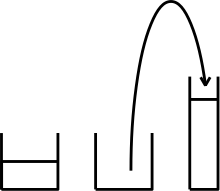
\includegraphics[width=7.5cm]{./images/papert-1/220px-Fig-2-mindstorms.png}
   \label{pap-1-1}
\end{figure}

Per un adulto è ovvio che versando liquido da un bicchiere ad un altro il volume del liquido non cambia (a meno di piccoli effetti, come gocce versate fuori o lasciate nel bicchiere precedente). La conservazione del volume è così ovvia che sembra non sia venuto in mente a nessuno prima di Piaget che ai bambini di quattro anni potrebbe apparire diversamente. Occorre una sostanziale crescita intellettuale prima che i bambini sviluppino una visione “conservazionista” del mondo. La conservazione del volume è solo una delle tante conservazioni che devono imparare.  Un'altra è la conservazione dei numeri. Anche in questo caso, gli adulti faticano a rendersi conto che un bambino   deve imparare il fatto che contando una collezione di oggetti in ordine diverso il risultato sia lo stesso. Per gli adulti l'operazione di contare significa semplicemente determinare quanti oggetti “ci sono”. Il risultato dell'operazione è un “fatto oggettivo” indipendente dall'atto di contare. Ma la separazione del numero dal conteggio (del prodotto dal processo) poggia su presupposti epistemologici che sono non solo ignoti al bambino preconservazionista, ma anche estranei alla loro visione del mondo. Tali conservazioni rappresentano solo una parte della vasta struttura di conoscenza matematica nascosta che i bambini imparano da soli. Nella geometria intuitiva del bambino di quattro o cinque anni, la linea retta non è necessariamente la distanza più breve fra due punti, e che camminare lentamente fra due punti non richiede necessariamente più tempo che camminare velocemente. Anche in questo caso, non è che manchi semplicemente un elemento di conoscenza, bensì il presupposto che sostiene l'idea “del più breve” quale proprietà di un percorso piuttosto che dell'azione di percorrerlo. 

Nessuno di questi casi deve essere interpretato come una carenza di conoscenza da parte del bambino. Piaget ha mostrato come i bambini piccoli abbiano teorie del mondo che, nei propri termini, sono perfettamente coerenti. Queste teorie sviluppate spontaneamente da tutti i bambini, hanno componenti ben sviluppati che non sono meno “matematici”, sebbene esprimano una matematica diversa, rispetto a quella accettata dalla nostra cultura (adulta). Il processo di apprendimento nascosto ha due fasi: già in età prescolare ogni bambino sviluppa teorizzazioni proprie del mondo per poi spostarsi verso visioni caratteristiche dell'età adulta. E questo accade attraverso quello che ho chiamato apprendimento piagetiano, un processo con caratteristiche che la scuola dovrebbe invidiare: funziona (accade in tutti i bambini), è economico (non richiede maestri ne curricula), e è “umano” (i bambini lo attuano con spirito apparentemente disinteressato senza bisogno di riconoscimenti o punizioni esplicite imposti dall'esterno).  

La misura in cui nella nostra società gli adulti hanno perso l'atteggiamento positivo dei bambini nei confronti dell'apprendimento varia da individuo a individuo. Una quota sconosciuta ma certamente significativa della popolazione ha completamente rinunciato a imparare. Queste persone raramente, se non mai, si cimentano nell'apprendimento e non si sentono né competenti né capaci di trarne giovamento. Il costo personale e sociale è enorme: la matofobia può limitare la vita delle persone, culturalmente e materialmente. Un numero ancora maggiore di persone non ha rinunciato completamente ma soffre di pesanti limitazioni a causa di pregiudizi negativi profondamente radicati sulle proprie capacità. La deficienza diventa identità: “Io non posso imparare il francese, non ho orecchio per le lingue;” “Non potrei mai fare affari, non ho la testa per i numeri.” “Non posso imparare lo sci parallelo, non sono mai stato coordinato.” Queste credenze sono spesso manifestate ripetutamente, in modo rituale, come superstizioni. E, come le superstizioni, creano un mondo di tabù; in questo caso il tabù dell'apprendimento. In questo capitolo e nel capitolo 3, discuteremo su degli esperimenti che dimostrano come queste immagini di se spesso corrispondano a una realtà molto limitata – usualmente la “realtà scolastica” di una persona. In un contesto formativo, con un adeguato supporto emozionale e intellettuale, lo “scoordinato” può imparare esercizi circensi come la giocoleria e coloro che “non hanno la testa per i numeri” possono scoprire che non solo sono in grado di capire la matematica ma vi si possono anche appassionare.

Sebbene tali opinioni negative su di se possano essere superate, di fatto sono estremamente tenaci e tendono ad autoconfermarsi. Se uno crede abbastanza fermamente di non poter fare matematica, avrà quasi sicuramente successo nell'impedirsi di fare qualsiasi cosa che gli paia attinente alla matematica. La conseguenza di tale autosabotaggio è il fallimento personale, e ogni fallimento rinforza l'assunto di base. Ancora più insidiosi sono i pregiudizi che appartengono non solo agli individui ma a un'intera cultura.

I nostri figli crescono in una cultura permeata dall'idea che ci siano “persone brillanti” e “persone stupide”. La costruzione sociale di un individuo è costituita da un fascio di attitudini. Ci sono persone “buone per la matematica”  e persone “negate per la matematica”. Tutto è aggiustato in maniera da attribuire i primi insuccessi o esperienze negative dei bambini a loro proprie disabilità. Di conseguenza, i bambini interpretano i fallimenti come sentenze di appartenenza al gruppo delle “persone stupide” o, più spesso, al gruppo delle persone “inadatte per l'attività x” (dove, come abbiamo osservato, spesso x si identifica con la matematica). In un contesto del genere i bambini declinano la propria personalità nei termini delle loro limitazioni, che verranno confermate e consolidate nel corso degli anni. Solo raramente accade che un evento eccezionale induca qualcuno a riorganizzare la propria immagine intellettuale in modo da aprire nuove prospettive su ciò che può apprendere.

Non è facile rimuovere questi pregiudizi sulla natura delle capacità umane. I pregiudizi popolari sono sempre difficili da sradicare. Ma qui le difficoltà sono sostenute da vari altri fattori. In primo luogo, le teorie comuni sulle attitudini umane sembrano essere sostenute da teorie “scientifiche”. Dopotutto, la psicologia si avvale molto di misure attitudinali. Proviamo a mettere in discussione la significatività di ciò che viene misurato mediante l'esperimento mentale di immaginare una \textit{Mathland}. 

Sebbene l'esperimento mentale lasci aperta la questione di come realizzarla una \textit{Mathland}, questo è tuttavia completamente rigoroso nel dimostrare che i pregiudizi comuni sulle capacità matematiche non sono sostenuti da evidenze palesi. Ma siccome i lettori più matofobici potrebbero avere problemi a fare l'esperimento per conto loro, lo riformulo in un altro modo. Immaginiamo di far disegnare ai bambini per un'ora al giorno passi di danza sulla carta e di far sostenere loro un esame su tali “questioni di danza” prima di lasciarli ballare veramente. Non dovremmo in tal caso aspettarci un mondo pieno di “danzofobi”? E non concluderemmo che coloro che ce la fanno a raggiungere la sala da ballo sono i più dotati per la danza? Io credo che sia altrettanto ingiustificato trarre conclusioni  sulle doti matematiche in base allo scarso entusiasmo dei bambini per passare centinaia di ore a fare somme.

Uno può sperare che passando dalle storie ai metodi più rigorosi della psicologia potremmo ottenere dati più consistenti sulle potenzialità degli individui in termini di competenze raggiungibili. Ma non è così: il paradigma corrente nella psicologia della formazione è focalizzato su come i bambini imparano o (più frequentemente) non imparano la matematica nella “anti-\textit{Mathland}” in cui viviamo. Un indirizzo che può essere descritto da questa storia:

\begin{quote}
Immaginiamo una persona del diciannovesimo secolo che volesse migliorare i sistemi di trasporto. Essa sarebbe stata probabilmente persuasa del fatto che la strada per escogitare nuovi metodi passi dalla conoscenza profonda dei metodi esistenti. Sarebbe così partita con uno studio accurato delle differenze fra i vari tipi di carri trainati da cavalli. Avrebbe quindi documentato accuratamente la dipendenza delle velocità ottenibili in funzione della forma e dei materiali degli assi, dei perni e delle finiture.
\end{quote}

Retrospettivamente sappiamo che la strada dell'evoluzione dei mezzi di trasporto è stata completamente diversa. Le invenzioni dell'automobile e dell'aeroplano non hanno preso le mosse dallo studio dettagliato su come i mezzi preesistenti, ovvero i carri trainati da animali, funzionassero o meno.  Ecco, questo è il  modello della ricerca attuale sulle questioni di formazione. I paradigmi usuali per tale tipo di ricerca pongono al centro degli  studi  la classe scolastica. Ci sono molti studi sullo scarso valore dell'insegnamento che viene impartito dalla scuola nella matematica e nelle scienze. È tuttavia diffusa l'idea che un “buon” approccio pedagogico debba basarsi su questi metodi, in realtà poveri di pensiero. Si può simpatizzare con le buone intenzioni, tuttavia penso che tali strategie riflettano il desiderio di mantenere il sistema tradizionale. Come dire di ritenere che convenga migliorare gli assi dei carri a trazione animale. Invece la questione importante sarebbe quella di inventare l'“automobile della formazione”. Questo problema (tema centrale di questo libro) non viene di fatto affrontato e, di conseguenza, ci sembra che le basi scientifiche che sostengono le assunzioni comuni sulle attitudini siano piuttosto labili. Assunzioni che tuttavia sono istituzionalizzate nelle scuole, nei sistemi di valutazione e di ammissione nelle università, al punto che la loro radicazione sociale è tanto forte quanto deboli sono i presupposti scientifici. 

Dalla scuola dell'infanzia in poi, i bambini sono sottoposti a prove basate su capacità verbali e quantitative concepite come entità “vere” e separabili. I risultati di tali test si trasformano in un corredo di attitudini che determinano la costruzione sociale del bambino. Una volta che Johnny e il suo maestro condividono la percezione che Johnny è una persona dotata per l'arte ma non per la matematica, tale percezione tende inevitabilmente a rinforzarsi con il tempo. Questo è un fatto largamente accettato nella psicologia della formazione. Ma il modo in cui la scuola forma le attitudini presenta aspetti più profondi. Consideriamo il caso di un bambino  che ho seguito durante i suoi ottavo e nono anni di età. Jim era un bambino molto loquace ma matofobico appartenente ad una famiglia di professionisti. La sua passione per le parole e il piacere di parlare si erano manifestate molto prima di andare a scuola. La matofobia era invece comparsa a scuola. La mia teoria è che essa sia stata una diretta conseguenza della sua precocità verbale. Dai genitori avevo appreso che Jim aveva presto sviluppato l'abitudine di commentare a voce alta qualsiasi cosa facesse. Un'abitudine che non aveva causato particolari problemi con i genitori o presso la scuola dell'infanzia. I problemi sono sorti affrontando l'aritmetica. A quel punto aveva già imparato a tenere sotto controllo la sua abitudine ma io sospetto che lui non avesse cessato di commentare le proprie azioni, seppur interiormente. Durante le ore di matematica si trovava in imbarazzo: semplicemente non riusciva a commentare l'attività di fare somme. Gli mancava il vocabolario (come manca alla maggior parte di noi) e non vedeva la motivazione. Questa frustrazione si tramutò in odio per la matematica, la conseguenza del quale fu una valutazione di scarsa attitudine per la materia. 

Per me fu una storia commovente. Credo che molto spesso quella che appare una debolezza intellettuale sia espressione, come nel caso di Jim, di quella che in realtà è una particolare capacità. È non è solo la capacità verbale, chiunque osservi con attenzione i bambini nota processi simili: per esempio un bambino che prediliga l'ordine logico può avere problemi con la sillabazione dell'inglese e magari finire col detestare la scrittura. L'idea di \textit{Mathland} ci suggerisce come il computer potrebbe servire ad evitare i problemi riscontrati da Jim e il suo pari dislessico. Ambedue i bambini sono vittime della netta separazione fra cultura verbale e matematica. Nella \textit{Mathland} che descriviamo in questo capitolo, la passione e la competenza verbale di Jim potrebbero essere mobilizzate per favorire lo sviluppo formale matematico, invece di ostacolarlo, e la passione dell'altro bambino per la logica potrebbe essere sfruttata per sviluppare le sue competenze linguistiche. 

Il concetto di mobilizzare tutte le capacità di un bambino per qualsiasi dominio di attività intellettuale risponde all'idea che attitudini differenti possano riflettere differenze nello sviluppo del cervello. È diventato comune ragionare come se ci fossero diversi cervelli, o diversi “organi” nel cervello. Per la matematica e per la lingua. In accordo con questo pensiero i bambini si dividono fra dotati per attività verbali o matematiche a seconda di quale loro organo cerebrale sia più forte. Ma una simile visione anatomica delle funzioni cerebrali comporta delle assunzioni epistemologiche. Per esempio si assume che si possa accedere alla matematica tramite una sola via e che se questa è “bloccata anatomicamente” allora il bambino non vi potrà accedere. Ora, di fatto, per la maggior parte dei bambini delle società contemporanee la via verso la matematica “avanzata” è una sola e questa è la via della matematica scolastica. Ma anche se ulteriori ricerche nella biologia del cervello arrivassero a dimostrare che tale via dipenda da un organo cerebrale  mancante in alcuni bambini, ciò non significa che la matematica stessa dipenda da organi del genere. Piuttosto, significherebbe che dovremmo cercare altre strade. La tesi sostenuta in questo libro è che esistano altre vie, e che la dipendenza delle funzioni dal cervello sia essa stessa un costrutto sociale

Supponiamo che esista una parte del cervello specializzata nelle manipolazioni mentali dei numeri che insegniamo scuola, e chiamiamola MAD, “\textit{Math Acquisition Device}”\footnote{[NdR] Qui Papert gioca con l'idea del linguista Noam Chomsky, secondo la quale il nostro cervello disporrebbe di una sorta di dispositivo di acquisizione del linguaggio (LAD: \textit{Language} \textit{Acquisition} \textit{Device}). Papert precisa di non credere a tale ipotesi, ritenendo un ipotetico MAD altrettanto improbabile di un LAD. Secondo l'ipotesi di Chomsky il cervello sarebbe composto da un insieme di organi neurologici specializzati per specifiche funzioni intellettuali. Secondo Papert tale ipotesi è troppo grossolana e se, probabilmente, si può ritenere che nel cervello vi siano dei dispositivi specializzati, è semplicistico immaginare che ve ne siano di così complessi da assolvere a funzioni quali il pensiero matematico e verbale.}. In tal caso nel corso dell'evoluzione umana si sarebbero sviluppati metodi per fare e insegnare l'aritmetica in grado di trarre massimo vantaggio dalle proprietà del MAD. Ma se questi metodi funzionassero solo per una parte di noi, e per la società nel suo insieme, si rivelerebbero invece catastrofici per un individuo il cui MAD fosse danneggiato o inaccessibile per qualche altro motivo (magari di origine “neurotica”). Una tale persona fallirebbe a scuola e le verrebbe diagnostica una “discalculia”. E finché noi insistiamo con l'insegnare l'aritmetica ai bambini nel modo convenzionale, continueremo a “dimostrare” tramite i test obiettivi che questi bambini non  possono “fare aritmetica”. Ma questo è come dimostrare che un bambino sordo non possa disporre di un linguaggio perché non sente. Così come la lingua dei segni impiega le mani e gli occhi per aggirare gli organi della parola, così si potrebbero individuare modi alternativi di fare matematica per aggirare il MAD, forse altrettanto validi anche se diversi. 

Ma non c'è bisogno di invocare la neurologia per spiegare come mai alcuni bambini non acquistano confidenza con la matematica. L'analogia con le lezioni di danza senza musica e senza sala da ballo è seria. La nostra cultura della formazione offre poche possibilità agli allievi di matematica per capire veramente ciò che studiano. Di conseguenza i nostri bambini sono forzati a seguire un modello di studio della matematica che è veramente il peggiore. È il modello dell'apprendimento mnemonico, dove i contenuti sono trattati come fossero privi di significato; è un modello “dissociato”. Alcune delle nostre difficoltà nell'insegnamento di una matematica culturalmente più integrabile sono dovute a un problema oggettivo: prima che esistessero i computer c'erano veramente pochi punti di contatto fra i fatti più importanti e coinvolgenti della matematica e l'esperienza quotidiana. Ma il computer – un'entità capace di parlare la matematica presente in modo ubiquitario nella vita di tutti i giorni a casa, nella scuola e al lavoro – può provvedere a tale collegamento. La sfida della formazione è quella di trovare i modi per sfruttare queste tecnologie.

La matematica non è certamente l'unico esempio di apprendimento dissociato. Ma è un ottimo esempio precisamente per il fatto che molti lettori preferirebbero che ora parlassimo d'altro. La nostra cultura è talmente  matofobica che se fosse possibile dimostrare come il computer potrebbe migliorare la nostra relazione con la matematica, avrei fondati motivi per sostenere che si potrebbero migliorare allo stesso modo le relazioni con altri tipi di apprendimento. Le esperienze in \textit{Mathland}, come quella di sostenere una “conversazione matematica”, fanno vivere all'individuo un senso liberatorio delle possibilità di fare una serie di cose che prima sembravano “troppo difficili”. In questo senso il contatto con il computer può aprire l'accesso alla conoscenza, non tanto in senso strumentale per disporre di informazioni processate, ma per porre in discussione alcune assunzioni vincolanti che le persone fanno su di se. La \textit{Mathland} del computer che propongo estende l'apprendimento naturale di tipo piagetiano dell'apprendimento della lingua madre all'apprendimento della matematica. L'apprendimento piagetiano è profondamente radicato in altri tipi di attività. Per esempio, i bambini piccoli non hanno momenti dedicati a “apprendere la lingua”.  Questo è un modello che si pone in contrapposizione all'apprendimento dissociato, che ha luogo in maniera relativamente separata da altre attività, mentali e fisiche. Nella nostra cultura, l'insegnamento della matematica a scuola è paradigmatico dell'apprendimento dissociato . Per la maggior parte della gente la matematica è insegnata e recepita come una medicina. La dissociazione matematica della nostra cultura è quasi una caricatura delle peggiori forme di alienazione epistemologica. Nell'ambiente LOGO si ammorbidiscono le distinzioni: nessuna attività in particolare è connotata a parte come “apprendere la matematica”. Il problema di rendere la matematica comprensibile concerne il problema più generale di rendere comprensibile un linguaggio basato su “descrizioni formali”. Così, prima di passare a esempi di come con il computer si possa provare a dare senso alla matematica, consideriamo alcuni esempi per rendere comprensibili linguaggi basati su descrizioni formali in domini della conoscenza che la gente non associa usualmente alla matematica. Nel primo esempio il dominio è quello della grammatica, per molti temibile quasi quanto la matematica.

Nel corso di uno studio di un anno, in una classe II di scuola  media di I grado di livello medio, una delle attività era quella che gli studenti chiamavano “\textit{computer} \textit{poetry}”. L'attività consisteva nell'usare il computer per comporre frasi: loro inserivano una struttura sintattica che il computer popolava di parole in maniera casuale. Il risultato è una sorta di poesia concreta tipo quella illustrata qui sotto\footnote{[NdR] Abbiamo lasciato la versione originale, ci pare inutile “tradurre” un pezzo simile, ai fini della comprensione del concetto.}:

\begin{quote}
INSANE RETARD MAKES BECAUSE SWEET SNOOPY SCREAMS\\
SEXY GIRL LOVES THATS WHY THE SEXY LADY HATES\\
UGLY MAN LOVES BECAUSE UGLY DOG HATES\\
MAD WOLF HATES BECAUSE INSANE WOLF SKIPS\\
SEXY RETARD SCREAMS THATS WHY THE SEXY RETARD\\
THIN SNOOPY RUNS BECAUSE FAT WOLF HOPS\\
SWEET FOGINY SKIPS A FAT LADY RUNS\\
\end{quote}

Un'allieva di tredici anni, Jenny, aveva commosso lo staff del progetto chiedendo il primo giorno: “Perché avete scelto noi? Noi non siamo i cervelloni. (“\textit{Why were we chosen for this? We're not the brains.}”. Lo studio prevedeva proprio di lavorare con una classe di livello “medio”. Un giorno Jenny entrò tutta eccitata. Aveva fatto una scoperta: “Ora ho capito perché ci  sono i sostantivi e i verbi.” Già da vari anni Jenny aveva fatto esercizi grammaticali, ma non aveva mai capito le differenze fra sostantivi, verbi e avverbi. Ma ora era chiaro che le sue difficoltà non dipendevano dall'incapacità di lavorare con categorie logiche. Il problema era un altro. Lei non aveva semplicemente compreso la finalità della fatica. Non era stata in grado di afferrare il senso della grammatica perché non vedeva a cosa servisse. E quando aveva chiesto a cosa serviva, la spiegazione dell'insegnante le era parsa manifestamente disonesta: “La grammatica ti serve a parlare meglio.”

Infatti, per recuperare la connessione fra l'apprendimento della grammatica e il miglioramento della lingua parlata occorre una visione più ampia del complesso procedimento di apprendimento di una lingua, che Jenny non poteva avere all'età in cui era entrata in contatto con la grammatica. Certamente lei non poteva vedere in che modo la grammatica potesse aiutarla a parlare meglio, né pensava di avere necessità di essere aiutata. Di conseguenza aveva sviluppato un sentimento di rancore per la grammatica. E, come succede alla maggior parte di noi, il rancore garantisce fallimento. Ma quando si è trovata nella condizione di far comporre frasi al computer, è successo qualcosa di interessante, trovandosi nella condizione di dover classificare le parole in categorie non perché qualcuno le avesse chiesto di farlo ma perché ne aveva bisogno. Per “insegnare” al suo computer come comporre serie di parole in maniera che sembrassero frasi compiute occorreva “insegnargli” a scegliere parole appartenenti alle categorie giuste. Ciò che lei aveva imparato sulla grammatica tramite l'esperienza con una  macchina non aveva niente di meccanico né di routinario. Il suo era stato un apprendimento profondo e significativo. Jenny aveva fatto più che imparare le definizioni per una particolare classe grammaticale. Aveva capito l'idea generale che le parole (come le cose) possono essere collocate in gruppi o insiemi diversi, e che fare questo può essere utile. Non aveva solo “capito” la grammatica ma aveva cambiato il suo atteggiamento nei suoi confronti. Era “sua”, e nel corso dell'anno, altri casi simili l'aiutarono rivedere la propria immagine. Cambiarono anche i suoi risultati; i suoi voti, prima medio-bassi, divennero massimi per il resto degli anni scolastici. Imparò che anche  lei poteva essere “un cervellone”, dopo tutto.

È naturale come matematica e grammatica non vengano capite dai bambini quando non sono capite da chi sta loro intorno e come, affinché la comprendano, occorra qualcosa di più di un insegnante che dica la cosa giusta o disegni il diagramma giusto alla lavagna. Ho chiesto a molti insegnanti e genitori cosa pensassero della matematica e perché fosse importante impararla. Pochi di loro hanno espresso una visione sufficientemente coerente da giustificare l'impiego di varie migliaia di ore della vita di un bambino per impararla, e questo i bambini lo sentono. Quando un insegnante spiega a uno studente che tutte quelle ore di aritmetica servono a essere in grado di controllare il resto al supermercato, questo non viene semplicemente creduto. I bambini interpretano tali “motivazioni” come un ulteriore esempio di malafede da parte degli adulti. Lo stesso effetto si manifesta dicendo ai bambini che la matematica scolastica è “divertente”, quando è loro chiaro che gli insegnanti che si esprimono così per divertirsi fanno tutt'altre cose. Ne aiuta molto spiegare che la matematica serve per diventare scienziati poiché la maggior parte di loro non prevede una cosa del genere.  La maggior parte dei bambini si rende conto che l'insegnante non ama la matematica più di quanto la amino loro e che la ragione per cui va fatta è semplicemente perché lo prevede il curricolo. Tutto ciò erode la fiducia dei bambini nel mondo degli adulti e nel processo di educazione. \textit{E io penso che introduca un elemento di profonda disonestà nella relazione educativa}\footnote{[NdR] Corsivo dell'autore.}.

I bambini percepiscono la retorica scolastica sulla matematica come un discorso in malafede. Al fine di rimediare la situazione dobbiamo prima riconoscere che la percezione dei  bambini è sostanzialmente corretta. Il “tipo di matematica” rifilata nelle scuole non è né significativa, né divertente e nemmeno utile. Ciò non significa che alcuni bambini non la possano vivere come un gioco personale importante e piacevole. Alcuni lo fanno per i voti; altri per barcamenarsi con l'insegnante e il sistema. Per molti, la matematica scolastica è piacevole proprio nella sua ripetitività, esattamente perché priva di significato e dissociata così da costituire un riparo da dover comprendere cosa stia accadendo in classe. Ma tutto questo mostra l'ingenuità dei bambini. Non si può giustificare la matematica scolastica sostenendo che, malgrado la sua intrinseca opacità, i bambini creativi vi trovino senso e divertimento.

È importante ricordarsi la distinzione fra matematica – un vasto dominio di indagine la cui bellezza è raramente immaginata da chi non è un matematico – e qualcos'altro che chiamerò “matematica scolastica”. 

Io interpreto la matematica scolastica come una costruzione sociale, una specie di QWERTY\footnote{[NdR] QWERTY denota la disposizione usuale delle tastiere, dalla prima linea di tasti in alto, leggendoli da sinistra verso destra. Papert in un'altra parte del libro (Cap. 1 – I computer e le culture del computer, pag. 32-34) descrive come tale disposizione si sia stabilita con le prime macchine da scrivere meccaniche, quando i tasti avevano una certa tendenza ad incepparsi. Per tale motivo prevalse empiricamente una disposizione che minimizzasse la battitura consequenziale di tasti adiacenti, circostanza che favoriva l'inceppamento. Ben presto l'evoluzione tecnica rese inutile tale accorgimento ma la disposizione QWERTY era ormai consolidata e sarebbe ormai stato antieconomico cambiare tutto il sistema, con una moltitudine di macchine a giro per il mondo è una competenza dattilografica ormai assestata su quello standard. Papert nota come universalmente si ritenga tale disposizione ottimale, sebbene non vi siano giustificazioni tecniche concrete a parte la motivazione iniziale ormai desueta, e utilizza, anche nel proseguio del libro, il “fenomeno QWERTY per connotare altri “intrappolamenti” del pensiero che vengono giustificati a posteriori con argomenti tecnici artificiosi quando invece le vere motivazioni consistono unicamente in varie forme di inerzia.}. Un insieme di accidenti storici (che discuteremo in breve) ha determinato la scelta degli argomenti matematici che dovrebbero costituire il bagaglio matematico di un cittadino. Come nel caso della disposizione QWERTY  dei tasti, la matematica scolastica ha avuto qualche senso in un certo contesto storico. Ma, analogamente, si è radicata così bene che tutti la danno per scontata, costruendo razionalizzazioni  per giustificarla, ben dopo la scomparsa delle condizioni storiche che l'avevano generata. Effettivamente, per la maggior parte della gente nella nostra cultura è inconcepibile che la matematica scolastica possa essere differente: questa è l'unica matematica che conoscono. Per tentare di rompere questo circolo vizioso, condurrò il lettore in un nuovo territorio matematico, la geometria della Tartaruga\footnote{[NrR] \textit{Turtle} \textit{geometry}.}, che con i miei colleghi abbiamo creato per dare ai bambini una prima introduzione più significativa al mondo della matematica formale. I criteri di progetto della geometria della Tartaruga si comprendono meglio esaminando più da vicino le circostanze storiche che hanno formato la matematica scolastica.

Alcune di queste circostanze erano pragmatiche. Prima che comparissero le calcolatrici elettroniche,   era una concreta necessità sociale quella di “programmare” molte persone affinché fossero in gradi di fare velocemente e accuratamente operazioni come lunghe divisioni. Ma ora che le calcolatrici sono accessibili economicamente dovremmo  riconsiderare l'utilità di dedicare svariate centinaia di ore della vita di ciascun bambino a imparare operazioni del genere. Non intendo negare il valore intellettuale di certa conoscenza, di molta conoscenza veramente, intorno ai numeri. Ben lungi da ciò. Ma possiamo selezionare questa conoscenza in base a criteri coerenti e razionali. Ci possiamo liberare dalla tirannia di considerazioni superficiali e pragmatiche che avevano determinato le scelte del passato su cosa debba essere imparato e a quale età.

Ma l'utilità era solo una delle motivazioni storiche per la matematica scolastica; altre erano di natura \textit{matetica}\footnote{[NdR] Corsivo dell'autore. Devoto Oli: Matetico. Nelle scienze e tecniche dell'educazione, che riguarda l'apprendimento, formativo: \textit{mezzi audiovisivi a scopo m.} [Dal gr. \textit{Máthēsis} 'apprendimento', per influsso dell'ingl. \textit{mathetic}].}. La matetica è l'insieme di principi guida che governano l'apprendimento. Alcune delle motivazioni storiche della matematica scolastica concernevano quello che poteva essere imparato e insegnato prima dell'avvento dei computer. Io credo che il fattore predominante che ha determinato quale matematica dovesse comporre la matematica scolastica fosse il contesto della classe scolastica dotata della tecnologia primitiva fatta di carta e matita. Per esempio, uno studente può disegnare un grafico con carta e matita. Così fu deciso di far disegnare molti grafici. Considerazioni simili hanno influenzato l'enfasi su certi tipi di geometria. Per esempio, nella matematica scolastica “geometria analitica” è diventata sinonimo di rappresentazione grafica delle equazioni. Il risultato è che ogni persona istruita si ricorda vagamente che $y = x^2$ rappresenta una parabola. E, sebbene la maggior parte dei genitori non abbia idea della ragione per cui ciò sia importante, questi si indignano se i anche i loro figli non lo imparano. Assumono che debbano esistere una ragione profonda e obiettiva, nota a coloro che conoscono meglio tali questioni. Ironicamente, è la propria matofobia che impedisce alle persone di esaminare tali ragioni più attentamente, trovandosi così alla mercé di sedicenti esperti di matematica. Pochissime  persone sospettano che la ragione per ciò che viene incluso o meno nella matematica scolastica è così banalmente tecnologica come la facilità con cui si disegna una parabola con carta e matita! Questo è quello che può cambiare così profondamente grazie ai computer: la varietà di costrutti matematici facilmente producibili è smisuratamente più ampia.

Un altro fattore matetico nella costruzione sociale della matematica scolastica è la tecnologia della votazione. Una lingua viva si impara parlando e non necessita di un insegnante che verifica e dà voti a ciascuna frase. Una lingua morta richiede invece un “riscontro” costante da parte di un insegnante. L'attività nota come “sommare” realizza un tale riscontro nella matematica scolastica. Questi piccoli esercizi ripetitivi assurdi hanno un solo merito: sono facili da valutare. E questo vantaggio li ha consolidati ben bene al centro della matematica scolastica. In sintesi, io ritengo che l'edificio della matematica scolastica sia fortemente influenzato da ciò che sembrava possibile insegnare quando la matematica veniva somministrata come una materia “morta”, usando tecnologie primitive di  tipo passivo, come sabbia e bastoni, lavagna e gesso, carta e matita. Il risultato è stato un insieme intellettualmente incoerente di argomenti che viola i più elementari  principi matetici in merito a cosa renda certi argomenti facili da imparare e altri quasi impossibili. 

A fronte dello stato di cose nella scuola, la formazione matematica può prendere due strade. Con l'approccio tradizionale la matematica scolastica viene data per scontata e ci si ingegna di insegnarla in qualche modo. Taluni usano i computer, ma, paradossalmente, l'impiego più comune è quello di impippiare materiale indigeribile, residuato dall'epoca pre-computer. Nella geometria della Tartaruga  il computer è usato in modo totalmente differente, come un mezzo matematicamente espressivo, che ci libera dalla necessità di individuare argomenti matematici possibili da imparare, significativi e intellettualmente coerenti. Invece di porre la questione di come insegnare la matematica scolastica esistente, poniamo quella di “ricostruire la matematica”, o più generalmente, di ricostruire la conoscenza in maniera che non debba essere così difficile insegnarla. 

Ogni “revisione del curriculum” potrebbe essere riformulata in termini di “ricostruzione della conoscenza”. Per esempio, con la riforma del curriculum \textit{New Math}\footnote{[NdR] Questo è palesemente un riferimento storico, da riferire all'epoca e da contestualizzare nella realtà americana.} degli anni Sessanta, qualche tentativo di cambiare i contenuti della matematica scolastica è stato fatto, ma non è cambiato molto. Le somme sono rimaste, anche se riformulate in modo un po' diverso. Il fatto che  le nuove somme si riferissero agli insiemi anziché ai numeri, o all'aritmetica in base 2 anziché in base 10 ha cambiato poco. Inoltre, la riforma della matematica scolastica non ha introdotto nessuna sfida attinente alla creatività dei matematici, non presentando così nessuna delle scintille che caratterizzano la formazione di pensiero nuovo. La denominazione stessa – \textit{New} \textit{Math} – si è rivelata impropria. C'era veramente poco di nuovo nei contenuti: niente di attinente a un processo di invenzione della matematica dei bambini, piuttosto ad una banalizzazione della matematica dei matematici. I bambini meritano qualcosa di meglio di una selezione di vecchia matematica. Come i vestiti passati dai fratelli maggiori, che non tornano mai bene. 

La geometria della Tartaruga ha presso le mosse con l'obiettivo di adattarsi ai bambini. Il primo criterio è quello della “appropriabilità”. Naturalmente i contenuti matematici devono essere pregnanti, ma vedremo che appropriabilità e pensiero matematico serio non sono affatto incompatibili. Al contrario: ci accorgeremo che alcune di tali personali conoscenze acquisite sono le più profondamente matematiche. In vari modi la matematica – per esempio la matematica dello spazio e del movimento, gli schemi ripetitivi delle azioni – è ciò che viene più naturale ai bambini. Lavorando insieme ai miei colleghi su queste idee, sono emersi alcuni concetti in grado di conferire più struttura al concetto di matematica appropriabile. In primo luogo, il principio di continuità: la matematica proposta deve essere in continuità con altre conoscenze, dalle quali possa ereditare un senso di familiarità e valore, insieme a competenza “cognitiva”. Poi il “principio di potenza”: dare allo studente il potere di affrontare progetti personali significativi, altrimenti impossibili. Infine il principio della “risonanza culturale”: gli argomenti devono avere senso in un contesto sociale allargato. Abbiamo parlato della geometria della Tartaruga che risulti comprensibile per i bambini. Ma questo non avverrà se non viene accettata anche dagli adulti. Una matematica di valore non può essere qualcosa che ci permettiamo di infliggere come fosse una medicina amara, e che non vediamo motivo di somministrare a noi stessi.












 %provvisorio
%\chapter{Il LOGO} \label{cap:papert2}

\section{prologo}

Questo è il capitolo successivo a quello sulla Mathophobia. È quello dove Papert introduce i comandi fondamentali di Logo. Dal punto di vista tecnico, è in parte una ripetizione del mio capitolo successivo (Disegnare), tuttavia, quest'ultimo è più ricalcato sullo stile del manuale di Lakó Viktória. La descrizione di Papert invece ha respiro molto più ampio perché da un lato concerne anche il metodo di insegnamento (come introdurre in pratica i comandi della Tartaruga ai bambini) e dall'altro offre vari interessanti collegamenti fra la Lingua della Tartaruga e la matematica formale. Quale leggere prima? Decida il lettore. I più frettolosi e interessati agli aspetti operativi possono saltare questo capitolo per passare direttamente a quello successivo, però se hanno un po' di tempo, secondo me farebbero meglio a seguire prima l'introduzione di Papert, penso che ne valga la pena. Così facendo si può tuttavia presentare il problema che Papert fa riferimento a frammenti di codice che questo manuale  non ha ancora presentato. Questi sono però intuitivi e invito il lettore ad accontentarsi della propria intuizione. Avrà modo di mettere a fuoco successivamente senza che la comprensione venga compromessa. Del resto è così che Papert introduce i comandi nel suo libro. Un'altra osservazione concerne la forma specifica dei frammenti di codice che non ho copiato pedissequamente, per due motivi. Il primo consiste nel problema appena menzionato, per cui ho introdotto qualche piccolo adattamento per facilitare la comprensione del lettore senza che venga alterato il messaggio fondamentale del testo. L'altro motivo consiste nel fatto che i codici scritti da Papert si riferiscono alla prima versione originale di Logo, che presenta qualche piccola differenza rispetto a quella che usiamo noi in LibreLogo. Ho quindi “tradotto” i frammenti di codice in maniera che possano essere copiati e eseguiti in un documento di LibreOffice.

\section{\textit{Turtle Geometry: A Mathematics Made For Learning}}

La geometria della Tartaruga è un modo diverso di fare geometria, come il modo assiomatico di Euclide e il modo analitico di Cartesio sono differenti fra loro. Quello di Euclide è un modo logico. Quello di Cartesio è un modo algebrico. La geometria della Tartaruga è un modo computazionale di fare geometria.

Euclide costruì la sua geometria a partire da un insieme di concetti fondamentali, uno dei quali è il punto. Il punto può essere definito come un'entità che ha posizione ma non ha altre proprietà – non ha colore, né misura, né forma. Le persone che non sono state iniziate alla matematica formale, che non sono state ancora “matematizzate”, hanno spesso difficoltà ad afferrare questa nozione, e la trovano bizzarra. È difficile per loro riferirla a qualcosa che conoscano. Anche la geometria della Tartaruga possiede un'entità fondamentale come il punto di Euclide. Ma questa entità, che io chiamo “Tartaruga”, può essere riferita a cose che le persone conoscono, perché a differenza del punto di Euclide, non è spogliata completamente da ogni altro attributo, e invece di essere statica e dinamica. Oltre alla posizione, la Tartaruga ha un'altra proprietà importante: ha “direzione”. Un punto euclideo si trova da qualche parte – ha una posizione e questo è tutto quello che se ne può dire. Una Tartaruga si trova da qualche parte – anch'essa ha una posizione – ma è anche rivolta da qualche parte – la sua direzione. In questo senso la Tartaruga è come una persona – io sono qui e sono rivolto a nord – o un animale o un battello. Ed è grazie a tali similitudini che la Tartaruga possiede la caratteristica speciale di fungere da prima rappresentazione formale per un bambino. I bambini si possono identificare con la Tartaruga e così sono in grado di traslare la conoscenza che hanno del loro corpo e di come si muovono nell'attività di apprendere la geometria formale.

Per sapere come funzioni dobbiamo imparare un'altra cosa sulle Tartarughe: la capacità di accettare comandi che sono espressi nella “Lingua delle Tartarughe”\footnote{[NdR] TURTLE TALK nell'originale.}. Il comando FORWARD fa muovere la Tartaruga lungo la direzione che sta puntando. Per dirle di quanto deve avanzare, FORWARD deve essere seguito da un numero: FORWARD 1 causa un movimento molto piccolo, FORWARD 100 un movimento più grande. In LOGO molti bambini sono stati iniziati alla geometria della Tartaruga mediante una tartaruga meccanica, sorta di robot cibernetico, in grado di obbedire ai comandi che vengono scritti su una tastiera\footnote{[NdR] Logo in realtà è nato negli anni '70 con questa versione meccanica che è quella rappresentata in Fig. 1. Tale versione è di fatto riemersa oggi nella forma dei robot didattici Bee-Bot e Blue-Bot. Ambedue possono ricevere i comandi mediante dei tasti che hanno sul dorso. Blue-Bot può essere manovrato attraverso un app per tablet o smartphone (sia Android che Apple) che consente di comporre un intero algoritmo e di scaricarlo mediante una connessione wireless nel Blue-Bot affinché lo esegua. Qui passato e presente si ricollegano e quello che sembrerebbe un riferimento datato è invece decisamente attuale.}. Questa “Tartaruga da pavimento” ha le ruote, una forma semisferica e una penna sistemata in maniera che la Tartaruga possa tracciare una linea muovendosi. Ma le sue proprietà essenziali – posizione, direzione e capacità di di eseguire i comandi della “Lingua delle Tartarughe” – sono quelle che contano per fare geometria. Il bambino può poi incontrare le medesime proprietà in un'altra materializzazione della Tartaruga, sorta di “Tartaruga leggera”. Questa è rappresentata da un oggetto triangolare su uno schermo televisivo\footnote{[NdR] È ovvio che lo “schermo televisivo” sia oggi sostituito dallo schermo di un computer. Inoltre, grazie alla smisurata potenza dei dispositivi di oggi, rispetto a quei tempi, il triangolo è oggi sostituito da immagini più dettagliate, quali la tartaruga stilizzata di LibreLogo o il “gatto” di Scratch. Abbiamo lasciato il testo originale per mettere in risalto il sapore pionieristico del racconto di Papert.  }, che possiede le stess proprietà di posizione e direzione e si muove in base agli stessi comandi della “Lingua delle Tartarughe”. Ambedue i tipi di Tartaruga hanno vantaggi: la Tartaruga da pavimento può essere usato come una ruspa o come uno strumento per disegnare; la Tartaruga leggera traccia brillanti linee colorate più velocemente di quanto l'occhio riesca a seguirle. Nessuna delle due è meglio di un'altra, ma insieme evocano un'idea potente: due entità fisicamente diverse possono essere matematicamente eguali (o “isomorfiche”)\footnote{Siccome questo libro è stato scritto per lettori che non sanno molta matematica, i riferimenti matematicamente più specifici sono limitati al massimo. Le osservazioni seguenti approfondiscono un po' il commento per i lettori più esperti.
L'isomorfismo fra i diversi tipi di Tartarughe è uno degli esempi di di idee matematiche “avanzate” che che nella geometria della Tartaruga emergono in forme che sono sia concrete che utili. Fra queste, quelle che ricadono nel dominio dell'analisi matematica sono particolarmente importanti.
Esempio 1: Integrazione. La geometria della Tartaruga apre la strada al concetto di integrale di linea attraverso le frequenti occasioni in che la Tartaruga ha di integrare qualche quantità mentre si muove. Di solito la prima circostanza in cui i bambini si imbattono compare con la necessità di di tenere traccia della somma delle rotazioni o della lunghezza totale percorsa. Un'eccellente progetto è quello dove si simulano i tropismi che inducono gli animali a cercare condizioni quali calore, luce, concentrazione di cibo, rappresentate mediante funzioni della posizione. Capita facilmente di confrontare due algoritmi per integrare una quantità lungo il percorso della Tartaruga. Una versione semplice dell'integrazione si può realizzare inserendo nel programma una singola linea del tipo CALL (TOTAL + FIELD) “TOTAL”, che significa: prendi la quantità che si chiama “TOTAL”, aggiungile la quantità FIELD e al risultato ridai il nome TOTAL. Questa versione ha un “difetto” ([NdR] bug) che si manifesta quando i segmenti percorsi dalla Tartaruga sono troppo lunghi oppure sono variabili. Risolvendo problemi del genere lo studente ha modo di avvicinarsi ad un concetto di integrale progressivamente più sofisticato.
La precoce introduzione di una versione semplificata dell'integrazione lungo un percorso illustra il rovesciamento di quello che sembrerebbe l'ordine pedagogico “naturale”. Nel curriculum tradizionale, l'integrale di linea è un argomento avanzato al quale gli studenti arrivano dopo essere stati indotti per vari anni a interpretare l'integrale definito come l'area sotto una curva, un concetto che sembra attagliarsi meglio alla tecnologia della carta e della matita. Ma il risultato è quello di di sviluppare una visione fuorviante dell'integrale che causa in molti studenti un senso di smarrimento quando incontrano integrali per i quali l'immagine dell'area sotto una curva è decisamente inappropriata. Esempio 2: Equazioni differenziali. Un progetto che colpisce molto gli studenti è quello della Tartaruga con Sensore Tattile ([NdR] Touch Sensor Turtle. I codici seguenti vanno letti in maniera indicativa, verranno compresi completamente più avanti nel manuale). La versione più semplice è di questo tipo:
TO BOUNCE
REPEAT		; Ciclo sulle istruzioni seguenti
 FORWARD 1		; La Tartaruga continua a muoversi
 TEST FRONT.TOUCH	; Controlla se sta battendo in qualcosa
 IFTRUE RIGHT 180	; Se sì torna indietro
END
Questo codice fa sì che la tartaruga torni indietro quando batte in un oggetto. Una versione più sofisticata e più istruttiva è questa:
TO FOLLOW
REPEAT
  FORWARD 1
  TEST LEFT.TOUCH	; Sta toccando l'oggetto?
  IFTRUE RIGHT 1	; È troppo vicino: mi allontano
  IFTRUE LEFT 1	; È troppo lontano: mi avvicino
END
Questo codice fa circumnavigare la Tartaruga intorno ad un oggetto di qualsivoglia forma, una volta che essa si trova con il suo lato sinistro a contatto dell'oggetto (e che l'oggetto e le irregolarità del suo contenuto siano grandi rispetto alla Tartaruga).
L'aspetto interessante di questi codici è quello di essere “locale”. Un comportamento “non locale” lo avremmo ottenuto per esempio se, dovendo circumnavigare un oggetto quadrato di lato pari a 150 passi, fossero state usate istruzioni del tipo FORWARD 150. Un approccio del genere manca di generalità: con altri oggetti potrebbe non funzionare. Invece i codici precedenti lavorano con piccoli passi decisi solo in base alle condizioni che si verificano nelle immediate vicinanze della Tartaruga. Invece dell'operazione “globale” FORWARD 150 usano solo operazioni “locali” come FORWARD 1.  In questo modo si impiega un concetto fondamentale della nozione di equazione differenziale. Ho visto bambini della scuola primaria capire perfettamente perché le equazioni differenziali sono la forma naturale delle leggi del moto. Anche questo è un esempio eclatante di inversione pedagogica: la potenza delle equazioni differenziali è compresa prima del formalismo dell'analisi matematica. Molte delle idee matematiche suggerite dalla Tartaruga sono riunite in H. Abelson e A. diSessa, Turtle Geometry: Computation as a Medium for Exploring Mathematics (Cambridge, MIT CERCARE!!!).
Esempio 3: Invarianti Topologici. Supponiamo che la Tartaruga giri intorno a un oggetto sommando via via gli angoli delle deviazioni, contando positivamente le deviazioni destre e negativamente quelle sinistre. Il risultato finale sarà sempre pari a 360 gradi indipendentemente dalla forma dell'oggetto. Vedremo che questo Total Turtle Trip Theorem è tanto utile quanto bello.}. 

I comandi FORWARD e BACK fanno muovere la tartaruga in linea retta lungo la propria direzione che sta puntando: cambia la posizione mentre la direzione rimane invariata. Ci sono altri due comandi che invece influiscono sulla direzione ma non sulla posizione: RIGHT  e LEFT fanno girare la Tartaruga su se stessa, cambiandone la direzione di puntamento ma non la posizione. Come nel caso dell'istruzione FORWARD, RIGHT e LEFT richiedono un numero che determina l'entità della rotazione. Un adulto interpreta immediatamente tale numero come l'angolo di rotazione espresso in gradi. Per i bambini invece questi numeri devono essere esplorati attraverso il gioco. 
Per disegnare un quadrato si può usare questo codice:

\begin{minipage}{0.5\textwidth}
\begin{figure}[H]
   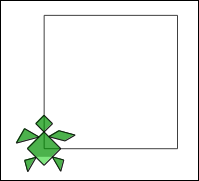
\includegraphics[width=5.0cm]{./images/papert-2/pap-2-1.png}
   \label{pap-2-1}
\end{figure}
\end{minipage} \hfill
\begin{minipage}{0.45\textwidth}
\begin{itemize}[itemsep=-3pt,parsep=2pt]
\item[] \hspace{0.5cm} FORWARD 100
\item[] \hspace{0.5cm} RIGHT 90
\item[] \hspace{0.5cm} FORWARD 100
\item[] \hspace{0.5cm} RIGHT 90
\item[] \hspace{0.5cm} FORWARD 100
\item[] \hspace{0.5cm} RIGHT 90
\item[] \hspace{0.5cm} FORWARD 100
\item[] \hspace{0.5cm} RIGHT 90
\end{itemize}
\end{minipage}
\\
\\
\\
Quello che segue è invece la trascrizione di un frammento dei tentativi di un bambino: 

\begin{minipage}{0.5\textwidth}
\begin{figure}[H]
   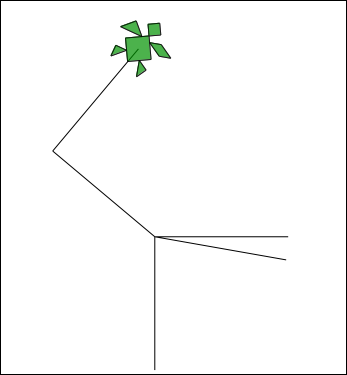
\includegraphics[width=5.0cm]{./images/papert-2/pap-2-2.png}
   \label{pap-2-2}
\end{figure}
\end{minipage} \hfill
\begin{minipage}{0.45\textwidth}
\begin{itemize}[itemsep=-3pt,parsep=2pt]
\item[] \hspace{0.5cm} FORWARD 100
\item[] \hspace{0.5cm} RIGHT 100
\item[] \hspace{0.5cm} FORWARD 100
\item[] \hspace{0.5cm} BACK 100
\item[] \hspace{0.5cm} 
\item[] \hspace{0.5cm} RIGHT 10
\item[] \hspace{0.5cm} LEFT 10
\item[] \hspace{0.5cm} LEFT 10
\item[] \hspace{0.5cm} FORWARD 100
\item[] \hspace{0.5cm} RIGHT 100
\item[] \hspace{0.5cm} LEFT 10
\item[] \hspace{0.5cm} 
\item[] \hspace{0.5cm} RIGHT 100
\item[] \hspace{0.5cm} LEFT 10
\item[] \hspace{0.5cm} FORWARD 100
\item[] \hspace{0.5cm} RIGHT 40
\item[] \hspace{0.5cm} FORWARD 100
\item[] \hspace{0.5cm} RIGHT 90
\item[] \hspace{0.5cm} FORWARD 100
\end{itemize}
\end{minipage}

Poiché imparare a controllare la Tartaruga è come imparare una lingua in questo modo si fa leva sulla capacità e l'inclinazione dei i bambini per l'espressione verbale. E siccome quelli che si devono dare alla tartaruga sono comandi, si fa leva sull'inclinazione dei bambini a impartire comandi. Per fare disegnare un quadrato alla Tartaruga, si può provare a camminare lungo il contorno di un quadrato immaginario e poi descrivere le operazioni fatte utilizzano la Lingua della Tartaruga. E così facendo, si fa leva sulle capacità motorie dei bambini e sul piaucere che provano nel muoversi. È un modo di impiegare la “geometria del corpo” propria del bambino come un punto di partenza per raggiungere la geometria formale. 


 va finito di portare da odt
\chapter{Il LOGO} \label{cap:papert2}

Questo capitolo è attualmente disponibile separatamente al seguente indirizzo: http://iamarf.ch/unifi/Papert-introduce-Logo.pdf.

Il motivo è che ne devo completare il porting verso il più professionale sistema di scrittura \LaTeX.

In una delle prossime revisioni verrà integrato adeguatamente tutto.
 
 %provvisorio
\chapter{Disegnare} \label{cap:disegnare}

\section{Comandi di movimento – Disegno - Uso delle variabili}

\subsection{I comandi fondamentali} \label{sec:comandi-fondamentali}

Il programma consente di creare grafica mediante il movimento di una  "tartaruga " che obbedisce a precisi comandi. Vediamo subito un esempio.

Apri un nuovo documento di testo e scrivi questo comando:

\vskip 1cm

\begin{scriptsize}
\begin{minipage}{01.0\textwidth}
\begin{itemize}[itemsep=-3pt,parsep=2pt]
\item[] \hspace{0.5cm} \textbf{HOME} 
\end{itemize}
\end{minipage}
\end{scriptsize}

\vskip 1cm

Vedrai che è apparsa la tartaruga in mezzo al foglio con la testa verso l'alto:

\begin{figure}[H]
   \centering
   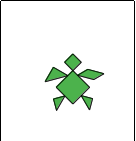
\includegraphics[width=3.0cm,trim=4 4 8 4,clip]{./images/disegnare/disegnare-1.png}
   \label{dis-1}
\end{figure}

Ora aggiungi un altro comando (d'ora in poi scriverò in grassetto solo i nuovi comandi che introdurremo):

\begin{scriptsize}
\begin{minipage}{0.45\textwidth}
\begin{itemize}[itemsep=-3pt,parsep=2pt]
\item[] \hspace{0.5cm} HOME 
\item[] \hspace{0.5cm} \textbf{FORWARD 100}
\end{itemize}
\end{minipage}
\end{scriptsize}
\begin{minipage}{0.5\textwidth}
\begin{figure}[H]
   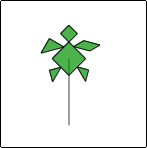
\includegraphics[width=3.0cm,trim=4 4 8 4,clip]{./images/disegnare/disegnare-2.png}
   \label{dis-2}
\end{figure}
\end{minipage} \hfill

\vskip 1cm

La tartaruga si è mossa tracciando una linea; è così che si disegna dando comandi alla tartaruga.
Scriviamo ora le seguenti istruzioni:

\vskip 1cm

\begin{scriptsize}
\begin{minipage}{0.45\textwidth}
\begin{itemize}[itemsep=-3pt,parsep=2pt]
\item[] \hspace{0.5cm} HOME 
\item[] \hspace{0.5cm} FORWARD 100
\item[] \hspace{0.5cm} \textbf{RIGHT 90}
\item[] \hspace{0.5cm} FORWARD 50
\item[] \hspace{0.5cm} \textbf{RIGHT 90}
\item[] \hspace{0.5cm} FORWARD 50
\item[] \hspace{0.5cm} \textbf{RIGHT 90}
\item[] \hspace{0.5cm} FORWARD 50
\item[] \hspace{0.5cm} RIGHT \textbf{90} 
\item[] \hspace{0.5cm} 
\end{itemize}
\end{minipage}
\end{scriptsize}
\begin{minipage}{0.5\textwidth}
\begin{figure}[H]
   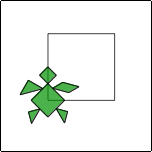
\includegraphics[width=3.0cm,trim=4 4 8 4,clip]{./images/disegnare/disegnare-3.png}
   \label{dis-3}
\end{figure}
\end{minipage} \hfill

\vskip 1cm

Abbiamo tracciato quattro lati, e alla fine di ogni lato abbiamo girato a destra di 90\degree, ottenendo così un quadrato.
  
Due parole sulla particolarità di LibreLogo.  La sequenza di istruzioni che abbiamo scritto è un frammento di codice, è software. L'abbiamo scritto in un particolare linguaggio, che è quello di Logo, ed è anche molto semplice, ma è software come qualsiasi altro. Di solito il software si scrive in appositi documenti mediante editori di testo semplice e si salvano in questo modo. Poi, si fanno eseguire al computer. I modi con qui si eseguono queste operazioni variano molto a seconda del tipo di linguaggio e di contesto. Oggi ci sono centinaia di linguaggi diversi che servono per gli scopi più disparati. La particolarità di LibreLogo è che il software si scrive in un documento e la tartaruga  "lavora " sul documento medesimo, lasciandovi la propria opera sotto forma di grafica, Così uno si ritrova insieme il codice e il risultato grafico prodotto da esso, in un unico documento. La grafica può essere selezionata con il mouse e, eventualmente, trasportata in contesti diversi. Ad esempio, le figure qui sopra le ho generate giocando con la tartaruga in un altro documento, poi ho selezionato le grafiche e le ho riportate qui. Un'altra notazione: un gruppo di istruzioni da fare funzionare in sequenza si chiama script, espressione che useremo diffusamente.

L'integrazione fra Logo e LibreOffice va oltre. È evidente che quando scriviamo il comando 

\vskip 1cm

\begin{scriptsize}
\begin{minipage}{1.0\textwidth}
\begin{itemize}[itemsep=-3pt,parsep=2pt]
\item[] \hspace{0.5cm} FORWARD 50  
\end{itemize}
\end{minipage}
\end{scriptsize}

\vskip 1cm

il numero 50 esprime la lunghezza del percorso che la tartaruga deve compiere. Puoi verificare subito cambiando il valore e guardando cosa fa la tartaruga. Ma cosa rappresenta quel 50?  Sono punti tipografici (point): 50 pt. Un punto sono 0.35 mm\footnote{La definizione precisa è: 1 pt = 1/72 polllici, dove 1 pollice = 25.4 mm. Quindi 1 pt = 2.54/72 = $.352\overline{7}$ mm}. LibreLogo capisce le unità di misura, si può scrivere 50, 50pt, 50mm, 50cm, 50in (inch: pollice), 50 " ( " sta per pollice). Ovviamente si tratta di lunghezze diverse. Usiamo per esempio i mm:

\vskip 1cm

\begin{scriptsize}
\begin{minipage}{0.45\textwidth}
\begin{itemize}[itemsep=-3pt,parsep=2pt]
\item[] \hspace{0.5cm} \textbf{CLEARSCREEN}
\item[] \hspace{0.5cm} HOME
\item[] \hspace{0.5cm} FORWARD \textbf{50mm}
\item[] \hspace{0.5cm} RIGHT 90
\item[] \hspace{0.5cm} FORWARD \textbf{50mm}
\item[] \hspace{0.5cm} RIGHT 90
\item[] \hspace{0.5cm} FORWARD \textbf{50mm}
\item[] \hspace{0.5cm} RIGHT 90
\item[] \hspace{0.5cm} FORWARD \textbf{50mm} 
\item[] \hspace{0.5cm} RIGHT 90     
\end{itemize}
\end{minipage}
\end{scriptsize}
\begin{minipage}{0.5\textwidth}
\begin{figure}[H]
   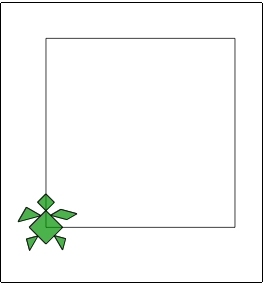
\includegraphics[width=5.0cm,trim=4 4 8 4,clip]{./images/disegnare/disegnare-4.png}
   \label{dis-4}
\end{figure}
\end{minipage} \hfill

\vskip 1cm

Il quadrato è ovviamente più grosso perché il precedente aveva il lato di 50 pt = 17.6 mm. 

Proviamo a complicare il disegno, immaginando di fare una casetta. La tartaruga si trova nel vertice in basso a sinistra e guarda in alto. Come prima cosa dobbiamo farla salire fino al vertice in alto a sinistra. Proviamo, e allo stesso tempo approfittiamo anche del fatto che le istruzioni possono essere raggruppate in una stessa riga, a seconda della convenienza:

\vskip 1cm

\begin{scriptsize}
\begin{minipage}{0.40\textwidth}
\begin{itemize}[itemsep=-3pt,parsep=2pt]
\item[] CLEARSCREEN             
\item[] HOME
\item[] FORWARD 50mm RIGHT 90
\item[] FORWARD 50mm RIGHT 90
\item[] FORWARD 50mm RIGHT 90
\item[] FORWARD 50mm RIGHT 90
\item[] FORWARD 50mm
\end{itemize}
\end{minipage}
\end{scriptsize}
\begin{minipage}{0.4\textwidth}
\begin{figure}[H]
   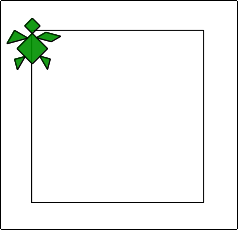
\includegraphics[width=5.0cm,trim=4 4 8 4,clip]{./images/disegnare/disegnare-5.png}
   \label{dis-5}
\end{figure}
\end{minipage} \hfill

\vskip 1cm

Non ci sono regole precise per raggruppare le istruzioni in una stessa riga. Il raggruppamento si può decidere in base alla comodità con cui si rilegge il codice. È importante facilitarsi la vita perché via via che il codice cresce può complicarsi rapidamente e tutti gli accorgimenti per renderlo più chiaro sono utili.

\vskip 1cm

\begin{minipage}{0.45\textwidth}
Ora dobbiamo costruire il tetto sulla casa. Facciamo questo appoggiando sul quadrato un triangolo equilatero, con la base coincidente con il lato superiore del quadrato. Essendo equilatero, anche gli altri due lati del triangolo saranno lunghi 50mm. Quindi per fare la falda sinistra del tetto la tartaruga dovrà spostarsi di 50mm ma deve prima cambiare direzione. Di quanto? Siccome gli angoli interni di un triangolo equilatero sono di 60\degree, la tartaruga dovrà deviare di 90\degree – 60\degree = 30\degree a destra. Arrivata in cima, disegnando la falda sinistra del tetto, dovrà girare a destra di 120\degree per poi disegnare la falda destra. Infine, girerà di 30\degree a destra per riallinearsi alla parete della casa.
\end{minipage}
\begin{minipage}{0.5\textwidth}
\begin{figure}[H]
   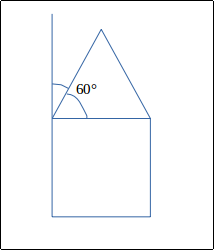
\includegraphics[width=6.5cm,trim=4 4 8 4,clip]{./images/disegnare/disegnare-6.png}
   \label{dis-6}
\end{figure}
\end{minipage} \hfill

\vskip 1cm

\begin{scriptsize}
\begin{minipage}{0.40\textwidth}
\begin{itemize}[itemsep=-3pt,parsep=2pt]
\item[] CLEARSCREEN             
\item[] HOME
\item[] FORWARD 50mm RIGHT 90
\item[] FORWARD 50mm RIGHT 90
\item[] FORWARD 50mm RIGHT 90
\item[] FORWARD 50mm RIGHT 90
\item[] FORWARD 50mm RIGHT 30
\item[] FORWARD 50mm RIGHT 120
\item[] FORWARD 50mm RIGHT 30
\end{itemize}
\end{minipage}
\end{scriptsize}
\begin{minipage}{0.4\textwidth}
\begin{figure}[H]
   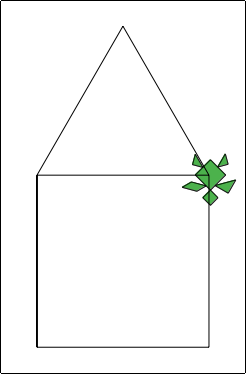
\includegraphics[width=5.0cm,trim=4 4 8 4,clip]{./images/disegnare/disegnare-7.png}
   \label{dis-7}
\end{figure}
\end{minipage} \hfill

\vskip 1cm

Supponiamo ora di voler disegnare una finestra nel mezzo della parete. Per fare questo è necessario introdurre due nuovi comandi - PENUP e PENDOWN – che consentono di muovere la tartaruga senza disegnare.

\vskip 1cm

\begin{scriptsize}
\begin{minipage}{0.40\textwidth}
\begin{itemize}[itemsep=-3pt,parsep=2pt]
\item[] CLEARSCREEN             
\item[] HOME
\item[] FORWARD 50mm RIGHT 90
\item[] FORWARD 50mm RIGHT 90
\item[] FORWARD 50mm RIGHT 90
\item[] FORWARD 50mm RIGHT 90
\item[] FORWARD 50mm RIGHT 30
\item[] FORWARD 50mm RIGHT 120
\item[] FORWARD 50mm RIGHT 120
\item[] \textbf{PENUP}
\item[] FORWARD 50mm/3 LEFT 90
\item[] FORWARD 50mm/3

dove abbiamo evidenziato in rosso il percorso fatto senza disegnare.
\end{itemize}
\end{minipage}
\end{scriptsize}
\begin{minipage}{0.4\textwidth}
\begin{figure}[H]
   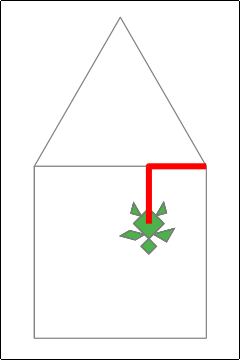
\includegraphics[width=5.0cm,trim=4 4 8 4,clip]{./images/disegnare/disegnare-8.png}
   \label{dis-8}
\end{figure}
\end{minipage} \hfill

\vskip 1cm

\begin{scriptsize}
\begin{minipage}{0.40\textwidth}
\begin{itemize}[itemsep=-3pt,parsep=2pt]
\item[] CLEARSCREEN             
\item[] HOME
\item[] FORWARD 50mm RIGHT 90
\item[] FORWARD 50mm RIGHT 90
\item[] FORWARD 50mm RIGHT 90
\item[] FORWARD 50mm RIGHT 90
\item[] FORWARD 50mm RIGHT 30
\item[] FORWARD 50mm RIGHT 120
\item[] FORWARD 50mm RIGHT 120
\item[] \textbf{PENUP}
\item[] FORWARD 50mm/3 LEFT 90
\item[] FORWARD 50mm/3
\item[] \textbf{PENDOWN}
\item[] FORWARD 50mm/3 RIGHT 90
\item[] FORWARD 50mm/3 RIGHT 90
\item[] FORWARD 50mm/3 RIGHT 90
\item[] FORWARD 50mm/3 RIGHT 90
\end{itemize}
\end{minipage}
\end{scriptsize}
\begin{minipage}{0.4\textwidth}
\begin{figure}[H]
   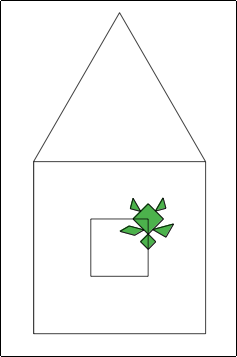
\includegraphics[width=5.0cm,trim=4 4 8 4,clip]{./images/disegnare/disegnare-9.png}
   \label{dis-9}
\end{figure}
\end{minipage} \hfill

\vskip 1cm

Proviamo ora ad arricchire ulteriormente il disegno, per esempio facendolo a colori.  

\vskip 1cm

\begin{scriptsize}
\begin{minipage}{0.40\textwidth}
\begin{itemize}[itemsep=-3pt,parsep=2pt]
\item[] CLEARSCREEN             
\item[] HOME
\item[] \textbf{PENCOLOR  "green "}
\item[] FORWARD 50mm RIGHT 90
\item[] FORWARD 50mm RIGHT 90
\item[] FORWARD 50mm RIGHT 90
\item[] FORWARD 50mm RIGHT 90
\item[] FORWARD 50mm RIGHT 30
\item[] \textbf{PENCOLOR  "red "}
\item[] FORWARD 50mm RIGHT 120
\item[] FORWARD 50mm RIGHT 120
\item[] PENUP
\item[] FORWARD 50mm/3
\item[] LEFT 90
\item[] FORWARD 50mm/3
\item[] PENDOWN
\item[] \textbf{PENCOLOR  "blue "}
\item[] FORWARD 50mm/3 RIGHT 90
\item[] FORWARD 50mm/3 RIGHT 90
\item[] FORWARD 50mm/3 RIGHT 90
\item[] FORWARD 50mm/3 RIGHT 90
\item[] \textbf{PENCOLOR  "gray "}
\end{itemize}
\end{minipage}
\end{scriptsize}
\begin{minipage}{0.4\textwidth}
\begin{figure}[H]
   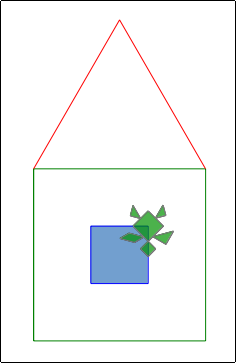
\includegraphics[width=5.0cm,trim=4 4 8 4,clip]{./images/disegnare/disegnare-10.png}
   \label{dis-10}
\end{figure}
\end{minipage} \hfill

\vskip 1cm

E perché non colorare anche l'interno?

\vskip 1cm

\begin{scriptsize}
\begin{minipage}{0.40\textwidth}
\begin{itemize}[itemsep=-3pt,parsep=2pt]
\item[] CLEARSCREEN            
\item[] HOME
\item[] FORWARD 50mm RIGHT 90
\item[] FORWARD 50mm RIGHT 90
\item[] FORWARD 50mm RIGHT 90
\item[] FORWARD 50mm RIGHT 90
\item[] FORWARD 50mm RIGHT 30
\item[] \textbf{FILLCOLOR  "yellow " FILL}
\item[] FORWARD 50mm RIGHT 120
\item[] FORWARD 50mm RIGHT 120
\item[] PENUP
\item[] FORWARD 50mm/3
\item[] LEFT 90
\item[] FORWARD 50mm/3
\item[] PENDOWN
\item[] \textbf{FILLCOLOR  "red " FILL}
\item[] FORWARD 50mm/3 RIGHT 90
\item[] FORWARD 50mm/3 RIGHT 90
\item[] FORWARD 50mm/3 RIGHT 90
\item[] FORWARD 50mm/3 RIGHT 90
\item[] \textbf{FILLCOLOR  "green " FILL}
\end{itemize}
\end{minipage}
\end{scriptsize}
\begin{minipage}{0.4\textwidth}
\begin{figure}[H]
   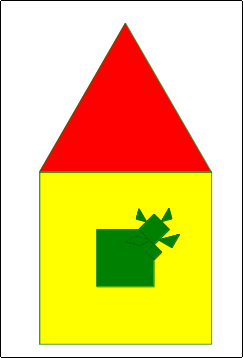
\includegraphics[width=5.0cm,trim=4 4 8 4,clip]{./images/disegnare/disegnare-11.png}
   \label{dis-11}
\end{figure}
\end{minipage} \hfill

\vskip 1cm

Anche in questo caso siamo ricorsi al raggruppamento delle istruzioni:
FILLCOLOR  "green " FILL. Con la prima si stabilisce il colore da usare
(FILLCOLOR  "green ") e con la seconda si procede a colorare la figura – viene
naturale inglobarle in una sola istruzione. 

L'istruzione FILL in realtà fa due cose: chiude una figura e la riempie di un
colore. Facciamo questa prova: 

\vskip 1cm

\begin{scriptsize}
\begin{minipage}{0.40\textwidth}
\begin{itemize}[itemsep=-3pt,parsep=2pt]
\item[] FORWARD 30mm RIGHT 90
\item[] FORWARD 30mm RIGHT 90
\end{itemize}
\end{minipage}
\end{scriptsize}
\begin{minipage}{0.4\textwidth}
\begin{figure}[H]
   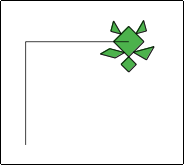
\includegraphics[width=5.0cm,trim=4 4 8 4,clip]{./images/disegnare/disegnare-12.png}
   \label{dis-12}
\end{figure}
\end{minipage} \hfill

\vskip 1cm

Così abbiamo disegnato una figura che non è chiusa. Volendo fare un triangolo potremmo far disegnare alla tartaruga il terzo lato. Alternativamente possiamo chiudere la figura con FILL, come abbiamo visto prima:

\vskip 1cm

\begin{scriptsize}
\begin{minipage}{0.40\textwidth}
\begin{itemize}[itemsep=-3pt,parsep=2pt]
\item[] FORWARD 30mm RIGHT 90
\item[] FORWARD 30mm RIGHT 90
\item[] FILL                  
\end{itemize}
\end{minipage}
\end{scriptsize}
\begin{minipage}{0.4\textwidth}
\begin{figure}[H]
   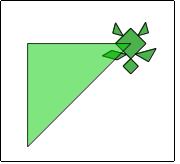
\includegraphics[width=5.0cm,trim=4 4 8 4,clip]{./images/disegnare/disegnare-13.png}
   \label{dis-13}
\end{figure}
\end{minipage} \hfill

\vskip 1cm

Così la figura è stata chiusa e colorata. Possiamo anche chiuderla senza
colorarla, usando l'istruzione \textbf{CLOSE}:

\vskip 1cm

\begin{scriptsize}
\begin{minipage}{0.40\textwidth}
\begin{itemize}[itemsep=-3pt,parsep=2pt]
\item[] FORWARD 30mm RIGHT 90
\item[] FORWARD 30mm RIGHT 90
\item[] CLOSE                  
\end{itemize}
\end{minipage}
\end{scriptsize}
\begin{minipage}{0.4\textwidth}
\begin{figure}[H]
   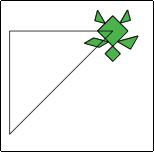
\includegraphics[width=5.0cm,trim=4 4 8 4,clip]{./images/disegnare/disegnare-14.png}
   \label{dis-14}
\end{figure}
\end{minipage} \hfill

\vskip 1cm

È interessante notare che, sia con FILL che con CLOSE la figura viene chiusa senza che la tartaruga  si sposti. Quindi se continuiamo ad aggiungere altri movimenti, questi prenderanno le mosse  da tale posizione della tartaruga, che negli esempi precedenti è rimasta volta verso il basso. Proviamo a mettere i due precedenti blocchi di codice uno dietro l'altro:

\vskip 1cm

\begin{scriptsize}
\begin{minipage}{0.40\textwidth}
\begin{itemize}[itemsep=-3pt,parsep=2pt]
\item[] FORWARD 30mm RIGHT 90
\item[] FORWARD 30mm RIGHT 90
\item[] FILL                  
\item[] FORWARD 30mm RIGHT 90
\item[] FORWARD 30mm RIGHT 90
\item[] CLOSE                  
\end{itemize}
\end{minipage}
\end{scriptsize}
\begin{minipage}{0.4\textwidth}
\begin{figure}[H]
   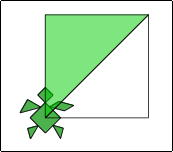
\includegraphics[width=5.0cm,trim=4 4 8 4,clip]{./images/disegnare/disegnare-15.png}
   \label{dis-15}
\end{figure}
\end{minipage} \hfill

\vskip 1cm

Dopo avere chiuso e colorato di verde il triangolo superiore, la tartaruga con le successive istruzioni di FORWARD procede a disegnare due lati del triangolo inferiore. L'istruzione CLOSE fa chiudere questo secondo triangolo senza colorarlo. 

E se uno volesse togliere la tartaruga una volta finito il disegno? Semplice: basta aggiungere alla fine l'istruzione \textbf{HIDETURTLE}. Prova! 

\subsection{I codici RGB per i colori}

Negli esempi precedenti abbiamo usato dei codici per esprimere i colori, per
esempio  "red " per indicare rosso. Si possono indicare così 24 colori: 

\vskip 1cm

\begin{figure}[H]
   \centering
   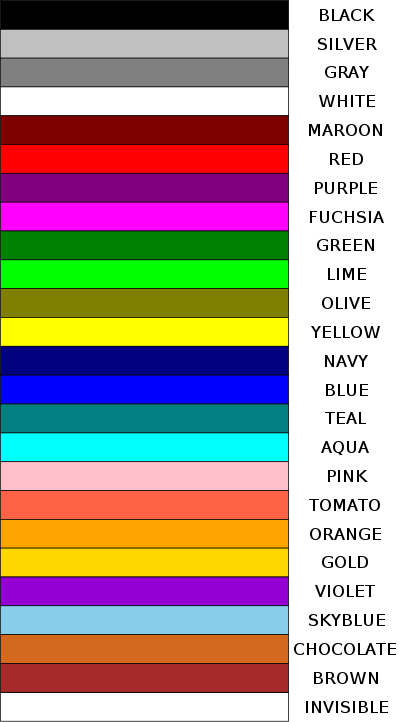
\includegraphics[width=8.0cm,trim=4 4 8 4,clip]{./images/disegnare/disegnare-16.png}
   \label{dis-16-a}
\end{figure}

In realtà i colori possibili sono molti di più. Questi possono essere espressi mediante il cosiddetto codice RGB, che sta per Red, Green, Blue. Nella grafica al computer i colori possono essere espressi come combinazione di tre colori fondamentali, che sono appunto rosso, verde e blu. Tutti gli altri possono essere espressi miscelando e dosando opportunamente questi tre colori fondamentali. Per fare questo si esprimono ile intensità dei singoli colori con un numero che va da 0 a 255 e si miscelano scrivendo ad esempio [255,0,0] per il rosso, [0,255,0] per il verde o [0,0,255] per il blu. Tutti gli altri colori si ottengono variando i valori all'interno delle parentesi. Con [0, 0, 0]  si ottiene il nero e con [255, 255, 255] il bianco. Poi questo tipo di codifica si utilizza in uno qualsiasi dei comandi che consentono di specificare il colore. Ad esempio

PENCOLOR [45, 88, 200]
FILLCOLOR [255, 200, 100]

Provate a giocare un po' con questi numeri per vedere che colori vengono fuori.

La tabella dei colori che abbiamo mostrato ha una stranezza: ci sono due elementi che hanno nome diverso ma il colore sembra lo stesso. Trovati? In realtà differiscono. ma per via di un quarto attributo, che è la trasparenza. Vediamo giocando un po'. 

Per facilitarci, anticipiamo un nuovo comando. Negli esempi precedenti noi abbiamo già disegnato un quadrato, utilizzando le istruzioni FORWARD e RIGHT, opportunamente combinate. In realtà, per disegnare le principali figure geometriche, in Logo esistono delle istruzioni preconfezionate, che ci aiutano a scrivere il codice in maniera più sintetica. Il quadrato è una di queste. Per fare un quadrato di 50 mm di lato si scrive:

\vskip 1cm

\begin{scriptsize}
\begin{minipage}{0.40\textwidth}
\begin{itemize}[itemsep=-3pt,parsep=2pt]
\item[] CLEARSCREEN
\item[] HOME
\item[] \textbf{SQUARE(30mm)}                            
\end{itemize}
\end{minipage}
\end{scriptsize}
\begin{minipage}{0.4\textwidth}
\begin{figure}[H]
   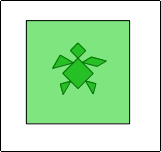
\includegraphics[width=5.0cm,trim=4 4 8 4,clip]{./images/disegnare/disegnare-17.png}
   \label{dis-16-b}
\end{figure}
\end{minipage} \hfill

\vskip 1cm

In questo modo la tartaruga disegna un quadrato e poi si piazza al centro con la testa rivolta in alto (il coloro non l'abbiamo determinato noi ma venuto  "automaticamente ", si dice che è il valore di default). Serviamoci allora di questa istruzione per disegnare prima un quadrato che coloriamo di rosso, poi spostiamoci un po' in basso e a destra, per disegnare un secondo quadrato, in modo che quest'ultimo si sovrapponga un poco al precedente, e poi lo coloriamo di bianco.

\vskip 1cm

\begin{scriptsize}
\begin{minipage}{0.40\textwidth}
\begin{itemize}[itemsep=-3pt,parsep=2pt]
\item[] CLEARSCREEN
\item[] HOME
\item[] FILLCOLOR [255, 0, 0]                                
\item[] SQUARE(50mm)
\item[] FORWARD -25mm
\item[] RIGHT 90                                             
\item[] FORWARD 25mm
\item[] FILLCOLOR [255, 255, 255]
\item[] SQUARE(50mm)                                         
\end{itemize}
\end{minipage}
\end{scriptsize}
\begin{minipage}{0.4\textwidth}
\begin{figure}[H]
   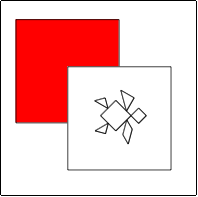
\includegraphics[width=5.0cm,trim=4 4 8 4,clip]{./images/disegnare/disegnare-18.png}
   \label{dis-17}
\end{figure}
\end{minipage} \hfill

\vskip 1cm

Bene, così il quadrato bianco si è sovrapposto a quello rosso. Un risultato prevedibile: i colori si sovrappongono perché sono opachi. Un pittore direbbe che  "coprono ". In realtà con i codici RGB in Logo si può assegnare un quarto parametro che è la  "trasparenza " che si vuole attribuire a quel certo colore, con la convenzione che un valore di 0 gli conferisce la completa opacità mentre il valore di 255 lo rende invece completamente trasparente. Con i valori compresi fra 0 e 255 si possono ottenere diversi livelli di trasparenza. Proviamo dunque a rendere trasparente il quadrato bianco, aggiungendo il quarto parametro uguale a 255:

\vskip 1cm

\begin{scriptsize}
\begin{minipage}{0.40\textwidth}
\begin{itemize}[itemsep=-3pt,parsep=2pt]
\item[] CLEARSCREEN
\item[] HOME
\item[] FILLCOLOR [255, 0, 0]                                
\item[] SQUARE(50mm)
\item[] FORWARD -25mm
\item[] RIGHT 90                                             
\item[] FORWARD 25mm
\item[] FILLCOLOR [255, 255, 255, 255]
\item[] SQUARE(50mm)                                        
\end{itemize}
\end{minipage}
\end{scriptsize}
\begin{minipage}{0.4\textwidth}
\begin{figure}[H]
   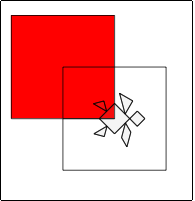
\includegraphics[width=5.0cm,trim=4 4 8 4,clip]{./images/disegnare/disegnare-19.png}
   \label{dis-18}
\end{figure}
\end{minipage} \hfill

\vskip 1cm

Il quadrato bianco è diventato trasparente. Se al posto di FILLCOLOR [255, 255, 255, 255] avessimo usato FILLCOLOR  "invisible " allora avremmo ottenuto lo stesso risultato. Ecco in cosa consiste la differenza fra il colore  "white " (bianco) e  "invisible ", invisibile, nella tabella che abbiamo visto all'inizio. 
Un'ultima annotazione. A guardare bene, si vede che in questi disegni ci ritroviamo con la tartaruga di colori diversi. Di fatto, la tartaruga viene colorata con lo stesso colore che abbiamo selezionato per riempire l'ultima figura disegnata, magari con una trasparenza diversa. Dopo avere disegnato il quadrato verde chiaro, la tartaruga è venuta verde un po' più scuro. Dopo il quadrato bianco è venuta grigio chiaro e dopo il colore invisibile e venuta grigio scuro. Questo è un comportamento che comunque non inficia i risultati che vogliamo ottenere perché qualora volessimo usare in qualche maniera le grafiche che produciamo, alla fine non avremo da fare altro che aggiungere l'istruzione HIDETURTLE.

\subsection{Altri comandi}

on i comandi di base che abbiamo visto fin qui è possibile produrre una gran quantità di grafiche. In Logo sono tuttavia disponibili dei comandi che consentono di abbreviare il disegno di alcune forma base. Abbiamo già anticipato l'istruzione SQUARE che consente di costruire un quadrato in un sol colpo. Le altre sono RECTANGLE, CIRCLE e ELLIPSE, che servono a costruire rispettivamente rettangoli, cerchi e ellissi.
Proviamo i seguenti comandi:

\vskip 1cm

\begin{scriptsize}
\begin{scriptsize}
\begin{minipage}{0.40\textwidth}
\begin{itemize}[itemsep=-3pt,parsep=2pt]
\item[] CLEARSCREEN
\item[] HOME
\item[] SQUARE 50                               
\item[] CIRCLE 50                                       
\end{itemize}
\end{minipage}
\end{scriptsize}
\end{scriptsize}
\begin{minipage}{0.4\textwidth}
\begin{figure}[H]
   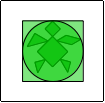
\includegraphics[width=3.0cm,trim=4 4 8 4,clip]{./images/disegnare/disegnare-20.png}
   \label{dis-19}
\end{figure}
\end{minipage} \hfill

\vskip 1cm

Si vede come l'effetto di disegnare due figure in sequenza sia quello di sovrapporle facendone coincidere il centro di simmetria e come la tartaruga si riposizioni sempre su tale centro. Si capisce anche come l'argomento\footnote{Con "argomento" si intende il valore che un comando richiede per essere effettuato. Gli argomenti possono essere anche più di uno – vedremo degli esempi. } del comando SQUARE rappresenti il lato del quadrato e quello del comando CIRCLE il diametro del cerchio che vogliamo costruire.

\vskip 1cm

\begin{minipage}{0.40\textwidth}
Prova a esercitarti con i comandi SQUARE e CIRCLE, per esempio costruendo la locomotiva qui accanto. Puoi esercitarti a rispettare delle proporzioni date, come quelle in questo esempio, dove il lato del quadrato più grande è due o tre volte quelli dei quadrati più piccoli e il diametro dei cerchi è pari al lato del quadrato più piccolo. A pagina nuova c'è una possibile soluzione, ma prima prova da solo. 
\end{minipage}
\begin{minipage}{0.4\textwidth}
\begin{figure}[H]
   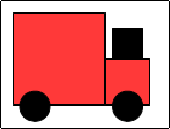
\includegraphics[width=5.0cm,trim=4 4 8 4,clip]{./images/disegnare/disegnare-21.png}
   \label{dis-20}
\end{figure}
\end{minipage} \hfill

\vskip 1cm

Una cosa importante di cui rendersi conto con il codice è che lo stesso obiettivo può essere conseguito in tanti modi diversi. Non esiste un criterio assoluto per stabilire quale sia il procedimento migliore. Quindi non esiste un'unica  "risposta giusta ". Un procedimento può essere meglio di un altro sotto un certo punto di vista: chiarezza del codice scritto, velocità di esecuzione, memoria totale impiegata dal codice, gestione di eventuali risorse ecc. Può succedere che un ottimo codice sotto uno di questi punti vista risulti pessimo sotto un altro.  

\newpage

\begin{scriptsize}
\begin{minipage}{0.40\textwidth}
\begin{itemize}[itemsep=-3pt,parsep=2pt]
\item[] COLOR  "red " 
\item[] SQUARE 60 
\item[] PENUP BACK 15 RIGHT 90 FORWARD 45                      
\item[] LEFT 90 PENDOWN 
\item[] SQUARE 30 
\item[] PENUP FORWARD 25 PENDOWN 
\item[] FILLCOLOR  "black "                      
\item[] SQUARE 20 
\item[] PENUP BACK 40 PENDOWN 
\item[] CIRCLE 20                                              
\item[] PENUP LEFT 90 FORWARD 60 PENDOWN 
\item[] CIRCLE 20
\item[] HIDETURTLE                                            
\end{itemize}
\end{minipage}
\end{scriptsize}

\vskip 1cm

Il quadrato e il cerchio hanno bisogno di un solo parametro per essere specificati. Invece, il rettangolo e l'ellisse hanno bisogno di due parametri. Nel caso del rettangolo i due parametri sono le lunghezze del lato lungo e del lato corto. L'istruzione per costruire un rettangolo è la seguente:

\textbf{RECTANGLE [60,40]}

Questo comando produce un rettangolo largo 60 punti e altro 40. Rispetto ai casi del quadrato de del cerchio questo comando ha un'altra particolarità: in questo caso, per fornire i due parametri necessari, si è ricorsi alla scrittura \textbf{[60,40]}. Questa è una  "lista " di valori. Si tratta di un modo per considerare un insieme di valori come un'unica cosa, una lista appunto, e il modo per ottenere questo effetto è quello di elencare i valori separandoli con le virgole e richiudendo tutto fra parentesi quadre. Le liste possono servire in varie circostanze, non solo in questo caso, ma vedremo successivamente come.
\textbf{Esercizio}: prova a realizzare un figura come questa qui sotto

\vskip 1cm

\begin{figure}[H]
   \centering
   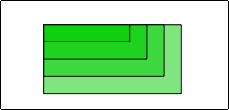
\includegraphics[width=4.0cm,trim=4 4 8 4,clip]{./images/disegnare/disegnare-22.png}
   \label{dis-21}
\end{figure}

\vskip 1cm

Anche in questo caso, prova da solo. Poi, a pagina nuova puoi vedere un possibile modo per risolverlo.

\pagebreak

\vskip 1cm
\begin{scriptsize}
\begin{minipage}{1.0\textwidth}
\begin{itemize}[itemsep=-3pt,parsep=2pt]
\item[] RECTANGLE [40mm, 20mm]
\item[] PENUP FORWARD 2,5mm LEFT 90
\item[] FORWARD 2,5mm RIGHT 90 PENDOWN   
\item[] RECTANGLE [35mm, 15mm]
\item[] PENUP FORWARD 2,5mm LEFT 90
\item[] FORWARD 2,5mm RIGHT 90 PENDOWN
\item[] RECTANGLE [30mm, 10mm]
\item[] PENUP FORWARD 2,5mm LEFT 90      
\item[] FORWARD 2,5mm RIGHT 90 PENDOWN
\item[] RECTANGLE [25mm, 5mm]
\item[] HIDETURTLE                      
\end{itemize}
\end{minipage}
\end{scriptsize}

\vskip 1cm

Un'altra figura che può tornare utile è l'ellisse. Detto nel più semplice dei modi l'ellisse è un cerchio schiacciato. È perfettamente nello spirito della geometria della Tartaruga quello di aiutarsi con riferimenti ad attività fisiche: probabilmente il miglior modo di usare le tecnologie moderne è di continuare ad utilizzare quelle tradizionali, integrando al meglio le une con le altre. Niente di meglio qui che farsi aiutare da Emma Castelnuovo\cite{Castelnuovo}, in un suo brano dove l'ellisse emerge studiando la classe di triangoli isoperimetrici con uguale base. Riportiamo il brano per intero, al fine di rispettare l'intento didattico di Emma, che è di valore:

\begin{quote}
Sempre un argomento di matematica, quale lo studio dei triangoli isoperimetrici con ugual base, porta a osservare quello che abbiamo sotto gli occhi. 

Il materiale è, anche questa volta, un pezzo di spago.

Per costruire dei triangoli di uguale base e uguale perimetro facciamo così: fissiamo due chiodi – siano A e B – su un tavolo su cui è disteso un foglio di carta; AB sarà la base dei nostri triangoli. Leghiamo poi gli estremi di un pezzo di spago ai due chiodi, tenendo presente che lo spago deve essere più lungo del tratto AB. Facciamo in modo, valendoci di una matita, che lo spago resti sempre ben teso e... lasciamoci guidare dalla matita.

Questa, guidata dallo spago, disegnerà sul foglio una curva a forma di ovale: è un'ellisse. I punti A e B si chiamano fuochi dell'ellisse. Dunque: i vertici dei triangoli isoperimetrici e di uguale base si trovano su un'ellisse.

Un problema di geometria ci ha condotti al disegno dell'ellisse. Con lo stesso pezzo di spago possiamo costruire un'ellisse più o meno  "schiacciata ", a seconda della distanza fra i punti A e B. Si può ottenere anche un cerchio, se i due punti coincidono: il cerchio, infatti, è un'ellisse particolare.    

L'ellisse, dopo averla incontrata in problemi di geometria, la ritroviamo per la strada, quando la  "calpestiamo " (perché un disco segnaletico dà, come ombra, un'ellisse. Nella nostra vita convulsa raramente ci soffermiamo a osservare l'ombra di un oggetto data dai raggi del soleo da una lampadina. Ma ecco che ora un'attività di geometria ci sollecita a guardare di più ed è proprio il confronto fra l'effetto-ombra dato dai raggi del sole e quello dato da una lampada puntiforme che stimola la nostra facoltà di osservazione. 

Guardiamo, ad esempio, due matite disposte in verticale su un tavolo. Se vengono illuminate dal sole accade che anche le ombre sono parallele; se invece è una lampada che le illumina le ombre si divaricano.

Da qui lo studio matematico delle trasformazioni affini e delle trasformazioni proiettive, fino ad arrivare alla prospettiva, all'arte, a come si guarda un quadro, alla storia.

È un piccolo problema di geometria che ha stimolato a osservare e a... guardarsi intorno.

\vskip 1cm

\begin{figure}[H]
   \centering
   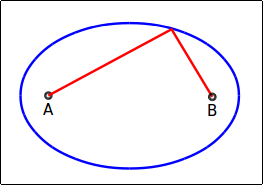
\includegraphics[width=8.0cm,trim=4 4 8 4,clip]{./images/disegnare/disegnare-23.png}
   \label{dis-22}
\end{figure}

\vskip 1cm

\end{quote}

In LibreLogo l'ellisse si disegna con il comando

\vskip 1cm

\begin{scriptsize}
\begin{minipage}{0.40\textwidth}
\begin{itemize}[itemsep=-3pt,parsep=2pt]
\item[] \textbf{ELLIPSE[40, 20]}
\end{itemize}
\end{minipage}
\end{scriptsize}

\vskip 1cm

L'ellisse ovviamente non ha un diametro fisso, come il cerchio. Per questo per essere definita richiede due parametri che sono i due assi, maggiore e minore. Nell'esempio l'ellisse ha l'asse maggiore uguale a 60 punti e il minore uguale a 40 punti. È possibile combinare le varie forme e aggiustare i loro parametri per ottenere una varietà di effetti. Per esempio un cerchio inscritto in un quadrato si può ottenere anche partendo dalle istruzioni per disegnare rettangoli e ellissi:

\vskip 1cm

\begin{scriptsize}
\begin{minipage}{0.40\textwidth}
\begin{itemize}[itemsep=-3pt,parsep=2pt]
\item[] RECTANGLE [60, 60] 
\item[] ELLIPSE [60, 60]   
\end{itemize}
\end{minipage}
\end{scriptsize}

\vskip 1cm

Prova a fare una figura come questa:

\vskip 1cm

\begin{figure}[H]
   \centering
   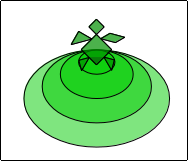
\includegraphics[width=4.0cm,trim=4 4 8 4,clip]{./images/disegnare/disegnare-24.png}
   \label{dis-23}
\end{figure}

\vskip 1cm
\pagebreak

Risposta possibile:

\vskip 1cm

\begin{scriptsize}
\begin{minipage}{0.40\textwidth}
\begin{itemize}[itemsep=-3pt,parsep=2pt]
\item[] ELLIPSE [120, 80] 
\item[] PENUP FORWARD 10 PENDOWN
\item[] ELLIPSE [90, 60]         
\item[] PENUP FORWARD 10 PENDOWN
\item[] ELLIPSE [60, 40] 
\item[] PENUP FORWARD 10 PENDOWN
\item[] ELLIPSE [30, 20] 
\item[] PENUP FORWARD 10 PENDOWN 
\end{itemize}
\end{minipage}
\end{scriptsize}

\vskip 1cm

Queste istruzioni consentono di usare anche altri parametro per ottenere delle varianti di rettangoli e ellissi. Nel caso dei rettangoli è possibile aggiustare un terzo parametro in maniera da arrotondare i vertici:

\vskip 1cm

\begin{scriptsize}
\begin{minipage}{0.40\textwidth}
\begin{itemize}[itemsep=-3pt,parsep=2pt]
\item[] RECTANGLE [60, 50, \textbf{10}]
\end{itemize}
\end{minipage}
\end{scriptsize}
\begin{minipage}{0.4\textwidth}
\begin{figure}[H]
   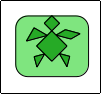
\includegraphics[width=3.0cm,trim=4 4 8 4,clip]{./images/disegnare/disegnare-25.png}
   \label{dis-24}
\end{figure}
\end{minipage} \hfill

\vskip 1cm

Supponiamo ora che un amico ci abbia appena detto di questa possibilità ma che altro non si ricordi. Si può controllare la  "rotondità " dei vertici? Probabilmente con quel terzo parametro, che l'amico ci ha detto potevamo fissare al valore di 10, ma come funziona? Questo è un ottimo esempio per mettere in luce lo strumento fondamentale di chi sviluppa software: la sperimentazione. Ecco, in questo caso, potremmo provare a fare dei tentativi, che potremmo (è solo una delle innumerevoli possibilità) sintetizzare così:

\vskip 1cm

\begin{scriptsize}
\begin{minipage}{0.40\textwidth}
\begin{itemize}[itemsep=-3pt,parsep=2pt]
\item[] FILLCOLOR  "invisible " 
\item[] PENCOLOR  "green " 
\item[] RECTANGLE [200, 150, 0] 
\item[] PENCOLOR  "black " 
\item[] RECTANGLE [200, 150, 10] 
\item[] RECTANGLE [200, 150, 20] 
\item[] RECTANGLE [200, 150, 30] 
\item[] RECTANGLE [200, 150, 40] 
\item[] RECTANGLE [200, 150, 50] 
\item[] RECTANGLE [200, 150, 60] 
\item[] RECTANGLE [200, 150, 70] 
\item[] RECTANGLE [200, 150, 80] 
\item[] RECTANGLE [200, 150, 90] 
\item[] RECTANGLE [200, 150, 100] 
\item[] PENCOLOR  "red " 
\item[] ELLIPSE [200,150]          
\end{itemize}
\end{minipage}
\end{scriptsize}
\begin{minipage}{0.4\textwidth}
\begin{figure}[H]
   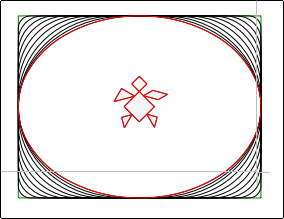
\includegraphics[width=5.0cm,trim=4 4 8 4,clip]{./images/disegnare/disegnare-26.png}
   \label{dis-25}
\end{figure}
\end{minipage} \hfill

\vskip 1cm
 
In questo modo ci siamo fatti un'idea di come possiamo controllare i rettangoli arrotondati. Ci siamo anche resi conto che, giocando con il terzo parametro, possiamo andare dal caso limite del rettangolo normale all'ellisse vera e propria.
Vediamo ora le varianti possibili per l'istruzione ELLIPSE.

\vskip 1cm

\begin{figure}[H]
   \centering
   \includegraphics[width=10.0cm,trim=8 8 8 8,clip]{./images/disegnare/disegnare-27.png}
   \label{dis-26}
\end{figure}

\vskip 1cm

Nell'istruzione ELLIPSE possiamo quindi utilizzare 3 parametri aggiuntivi, che servono a disegnare solo un settore dell'ellisse. I primi due rappresentano l'angolo iniziale e finale, espressi in gradi, che delimitano il settore. Nell'esempio sopra, avendo scelto 0 e 90 abbiamo imposto di disegnare il primo quadrante dell'ellisse. Il quarto parametro stabilisce se si vuole disegnare un settore di ellisse (1), un segmento di ellisse (2) oppure giusto un arco (3).

\subsection{Le variabili} \label{sec:variabili}

 Le istruzioni che abbiamo visto sin'ora consentono di fare molte cose: abbiamo imparato a muovere la tartaruga in ogni parte del foglio, a farla disegnare o meno, abbiamo visto come controllare il colore del tratto e il riempimento delle figure. Si potrebbe avere la sensazione che per produrre grafica non occorra altro. Invece abbiamo solo scalfito la superficie delle potenzialità di un linguaggio di programmazione, anche se questo ha finalità esclusivamente didattiche, come nel caso di Logo e dei suoi derivati. Introdurremo via via le caratteristiche più importanti. Fra queste la prima, che ci serve subito per poter andare avanti,  è il concetto di  "variabile ". Fin qui abbiamo usato varie istruzioni che richiedono degli  "argomenti ". L'argomento è il valore che un'istruzione può richiedere per poter essere eseguita. Ad esempio l'istruzione FORWARD non avrebbe senso senza un argomento che rappresenti la distanza che la tartaruga deve percorrere. L'espressione FORWARD 50  significa che la tartaruga deve muoversi in avanti di 50 punti; 50 è il valore dell'argomento. Vi sono anche istruzioni che richiedono più di un argomento, è per esempio il caso di RECTANGLE e ELLIPSE. In ogni caso, in tutti gli esempi visti precedentemente abbiamo sempre usato argomenti numerici per tutte le istruzioni. In realtà, tutti i linguaggi consentono di servirsi di un'importante generalizzazione che consiste nell'uso delle  "variabili ". Si tratta di nomi simbolici ai quali possono essere assegnati vali numerici a piacimento. Proviamo ad eseguire il seguente codice:

\vskip 1cm

\begin{scriptsize}
\begin{minipage}{0.40\textwidth}
\begin{itemize}[itemsep=-3pt,parsep=2pt]
\item[] CLEARSCREEN
\item[] HOME
\item[] 
\item[] LATO = 100
\item[] ANGOLO = 90
\item[] 
\item[] FORWARD LATO
\item[] LEFT ANGOLO
\item[] FORWARD LATO
\item[] LEFT ANGOLO
\item[] FORWARD LATO
\item[] LEFT ANGOLO
\item[] FORWARD LATO
\item[] HIDETURTLE    
\end{itemize}
\end{minipage}
\end{scriptsize}
\begin{minipage}{0.4\textwidth}
\begin{figure}[H]
   \includegraphics[width=3.0cm,trim=4 4 8 4,clip]{./images/disegnare/disegnare-28.png}
   \label{dis-27}
\end{figure}
\end{minipage} \hfill

\vskip 1cm

Abbiamo disegnato un quadrato, ma invece di utilizzare direttamente il valore 100 come argomento delle istruzioni FORWARD, abbiamo prima assegnato il valore 100 alla variabile di nome  "LATO " e poi abbiamo utilizzato questa come argomento di tutte le istruzioni FORWARD. È evidente quale possa essere l'utilità di questo metodo: supponiamo che non sia soddisfatto delle dimensioni di questo quadrato e che voglia provare altri valori del lato. Ebbene, non ho altro che da cambiare il valore 100 nell'istruzione LATO = 100, cambiandola per esempio con LATO = 150. Prova a sperimentare! Puoi anche cambiare il valore di ANGOLO, sperimentando con valori diversi... 
Coloro che hanno studiato i primi rudimenti dell'algebra, avranno certamente riconosciuto il concetto di variabile, che in quella disciplina si utilizza ampiamente per eseguire calcoli simbolici. Si ricorderanno anche che il concetto di variabile si declina in vari modi, per esprimere quantità che si considerano effettivamente variabili – ad esempio una variabile dipendente in funzione di altre variabili indipendenti – poi quantità che si assumono costanti, infine quantità che assumono il significato di parametri, che sono come costanti che possiamo avere interesse a cambiare di tanto in tanto. In ogni caso tutte queste quantità vengono rappresentate in maniera simbolica. In realtà, coloro che hanno poi avuto modo di approfondire lo studio dell'algebra, sanno che il  concetto di variabile è passibile di tutta una serie di generalizzazioni. Niente paura, questo non è un corso di matematica sottobanco, o forse un po' sì: in fin dei conti Logo rappresenta l'anelito di Seymour Papert di rendere la matematica più accessibile. Ma ciò che proponiamo qui non richiede doti o attitudini particolari. Introduciamo solo una delle generalizzazioni possibili, che ci servirà immediatamente. La generalizzazione che proponiamo attiene al concetto di posizione della tartaruga nel foglio. La posizione lungo una linea è determinata da un semplice numero – ad esempio la posizione lunga una strada:  "si segnalano lavori in corso al Km 287... ". Diverso è il caso della posizione su di una superficie. In un  navigatore satellitare, che oggi tutti conoscono, si può dare anche la posizione in termini geografici, ma questa deve essere somministrata mediante due valori: la latitudine e la longitudine, che designano il parallelo terrestre la prima e il meridiano la seconda. Per affondare una nave nel gioco della battagli navale occorre fornire due coordinate, per esempio b7, dove  "b rappresenta la colonna e 7 la riga. Allo stesso modo si identificano le celle di un foglio di lavoro, e via dicendo. Anche alla nostra tartaruga occorrono due valori numerici per identificare una posizione precisa nel foglio, che possiamo immaginare come la x e la y della tartaruga nello spazio della pagina. Ebbene, il modo per esprimere questo concetto nel mondo della tartaruga (ma non solo!) è il seguente:

\vskip 1cm

\begin{scriptsize}
\begin{minipage}{0.40\textwidth}
\begin{itemize}[itemsep=-3pt,parsep=2pt]
\item[] P=[200, 300]
\item[] PRINT P
\end{itemize}
\end{minipage}
\end{scriptsize}

\vskip 1cm

Se si esegue questo codice, LibreLogo stampa il  "valore " [200, 300]. Ovviamente abbiamo scelto questi numeri in maniera del tutto arbitraria, giusto per fare un esempio. Lo scopo è quello di mostrare come si rappresenta in maniera simbolica una posizione, che in realtà è espressa mediante un insieme di due numeri. Nell'algebra si dice che questo tipo di variabile è un  "vettore ". C'è anche un modo per  "isolare " i singoli elementi all'interno di un vettore. La cosa si descrive subito con questo esempio:

\vskip 1cm

\begin{scriptsize}
\begin{minipage}{0.40\textwidth}
\begin{itemize}[itemsep=-3pt,parsep=2pt]
\item[] P=[200, 300]
\item[] PRINT P
\item[] PRINT P[0]
\item[] PRINT P[1]
\end{itemize}
\end{minipage}
\end{scriptsize}

\vskip 1cm

Se si esegue questo frammento di codice, prima viene stampato  "valore " [200, 300], poi il valore 200, quindi 300. Da qui si capisce che con P [0] si ottiene il primo elemento del vettore posizione, che contiene il numero 200, e con P [1] il secondo elemento, che contiene il numero 300.
Ecco, questo è quanto dovrebbe bastare per andare a vedere com'è che si può controllare con ancora maggiore agilità la posizione della tartaruga nel foglio. 

\subsection{Lo spazio della pagina} \label{se:spazio-pagina}

Abbiamo già visto vari comandi per muovere la tartaruga ma sono tutti finalizzati al disegno. È vero che si possono fare i movimenti con la  "penna alzata " (comando PENUP) ma può essere utile  "saltare " direttamente in una posizione qualsiasi del foglio, oppure puntare in una direzione precisa.  Si tratta, in altre parole, di scegliere una posizione o una direzione in termini assoluti e non in modo relativo, rispetto alla posizione e direzione corrente, come si fa per esempio con istruzioni del tipo FORWARD oppure LEFT. Qui sorge la necessità di utilizzare dei  riferimenti spaziali assoluti che sono una coppia di coordinate per la posizione nel foglio e un angolo per la direzione. Per sapere come funzionano tali riferimenti introduciamo e usiamo subito due nuove istruzioni: \textbf{POSITION}  e \textbf{HEADING}. Inoltre, ci è utile anche l'istruzione \textbf{PRINT}, per conoscere il valore corrente della posizione e della direzione. Infatti i due comandi \textbf{POSITION} e \textbf{HEADING}, si possono usare con e senza parametri. Quando si usano senza parametri allora questi forniscono i valori correnti. Infatti, se apro un nuovo documento in Writer e faccio eseguire il comando

\vskip 1cm

\begin{scriptsize}
\begin{minipage}{1.0\textwidth}
\begin{itemize}[itemsep=-3pt,parsep=2pt]
\item[] \textbf{PRINT POSITION}
\end{itemize}
\end{minipage}
\end{scriptsize}

\vskip 1cm

si ottiene la seguente risposta:

\vskip 1cm

\begin{figure}[H]
   \centering
   \includegraphics[width=10.0cm,trim=8 8 8 8,clip]{./images/disegnare/disegnare-28.png}
   \label{dis-28}
\end{figure}

\vskip 1cm

I due numeri fra parentesi rappresentano le coordinate x e y della posizione nello spazio della pagina: 298 e 421\footnote{Abbiamo arrotondato i due numeri a quattro cifre significative, che sono adeguate a determinare la posizione nel foglio, ai nostri fini. Nella nota successiva diamo una breve spiegazione dell'unità di misura impiegata per questi numeri.} rispettivamente. Dal momento che abbiamo appena aperto il documento e che all'inizio la tartaruga viene piazzata al centro, possiamo assumere che queste coordinate rappresentino il centro della pagina. Tuttavia, per avere il controllo completo della situazione occorre conoscere precisamente l'estensione dello spazio dell'immagine.  Ebbene, le coordinate dell'angolo superiore sinistro sono [0, 0], dove il primo numero rappresenta la coordinata x e il secondo la y, mentre quelle dell'angolo inferiore destro si ottengono stampando il valore della variabile speciale \textbf{PAGESIZE}, che LibreLogo utilizza per conservare le dimensioni della pagina. In questo momento la mia versione di Writer è predisposta per pagine di dimensioni A4 e, conseguentemente, eseguendo l'istruzione 

\vskip 1cm

\begin{scriptsize}
\begin{minipage}{1.0\textwidth}
\begin{itemize}[itemsep=-3pt,parsep=2pt]
\item[] \textbf{PRINT PAGESIZE}
\end{itemize}
\end{minipage}
\end{scriptsize}

\vskip 1cm

otteniamo:

\vskip 1cm

\begin{figure}[H]
   \centering
   \includegraphics[width=10.0cm,trim=8 8 8 8,clip]{./images/disegnare/disegnare-29.png}
   \label{dis-29}
\end{figure}

\vskip 1cm

Questi numeri, arrotondati, 596 e 842, rappresentano le dimensioni di un foglio A4 espressi in  "punti " alla densità di 72 DPI/footnote{L'acronimo DPI sta per dots per inch: punti per pollice. Il valore di DPI dipende dal supporto fisico su cui si intende che un'immagine debba essere rappresentata. Poiché un pollice vale 2.54 cm, la densità di 72 DPI corrisponde a 72/2.54 = 28.3 punti per cm, o 2.83 punti per mm; giusto per avere un riferimento a noi più famigliare. Quando in Writer si sceglie l'unità di misura  "punti " (anziché cm o pollici), questi si riferiscono alla densità di 72 DPI appena citata. In Writer, l'unità di misura si può cambiare con la voce di menu Tools->Options->LibreOffice Writer->General. Si può scegliere fra mm, cm, pollici, pica, punti.}. In mm risultano 210 e 297 mm. Riassumiamo la situazione con la seguente figura.

\vskip 1cm

\begin{figure}[H]
   \centering
   \includegraphics[width=10.0cm,trim=8 8 8 8,clip]{./images/disegnare/disegnare-30.png}
   \label{dis-30}
\end{figure}

\vskip 1cm

Tutte le volte che vogliamo utilizzare le posizioni assolute possiamo fare riferimento a questo schema che ci fornisce l'orientamento del sistema di riferimento sul foglio e le sue dimensioni. Nella tabella successiva vediamo i valori numerici corrispondenti:

\begin{center}
%\begin{tabular}{| >{\centering\arraybackslash}m{1in} | >{\centering\arraybackslash}m{1in} |}
\begin{tabular}{| l | l |}
\hline
[0, 0] & [0, 0] \\ \hline
[PAGESIZE[0], 0]  & [596, 0] \\ \hline 
[0, PAGESIZE[1]]  &     [0, 842]   \\ \hline 
[PAGESIZE[0], PAGESIZE[1]]  & [596, 842]   \\ \hline 
\end{tabular}
\end{center}

Riallacciandosi al paragrafo precedente, PAGESIZE è una variabile, una variabile che all'interno di LibreLogo è trattata come una costante perché contiene le dimensioni della pagina. Inoltre è quel particolare tipo di variabile che si chiama vettore, perché composta da più elementi, precisamente due, le due dimensioni della pagina: PAGESIZE[0] è la larghezza e PAGESIZE[1] la lunghezza.
Come facciamo dunque per spedire la tartaruga in una posizione precisa?

\vskip 1cm

\begin{figure}[H]
   \centering
   \includegraphics[width=10.0cm,trim=8 8 8 8,clip]{./images/disegnare/disegnare-31.png}
   \label{dis-31}
\end{figure}

\vskip 1cm

Con l'istruzione \textbf{POSITION [350, 320]} la tartaruga si dirige direttamente al punto di coordinate \textbf{POSITION [[350,320]}, a partire dal punto dive si trova, in questo caso dal centro della pagina.

Come possiamo usare l'istruzione POSITION per controllare la posizione, in modo analogo possiamo utilizzare l'istruzione HEADING per controllare la direzione in cui punta la tartaruga. Invocando l'istruzione HEADING senza alcun parametro si ottiene la posizione corrente. Utilizzando invece un parametro, per esempio HEADING [30], si impone alla tartaruga di ruotare di 30\degree. Nella figura seguente si mostra l'orientamento del sistema di riferimento.

\vskip 1cm

\begin{figure}[H]
   \centering
   \includegraphics[width=10.0cm,trim=8 8 8 8,clip]{./images/disegnare/disegnare-32.png}
   \label{dis-32}
\end{figure}

\vskip 1cm

Quando si apre un documento nuovo, oppure dopo l'istruzione HOME, la tartaruga punta verso il lato superiore del foglio, e questa direzione corrisponde a 0\degree.

\subsection{Altri comandi grafici}

È possibile controllare anche altri aspetti del disegno, oltre al colore.

\subsubsection{PENWIDTH (spessore tratto)}

Con il comando \textbf{PENWIDTH} si determina lo spessore del tratto:


\vskip 1cm

\begin{figure}[H]
   \centering
   \includegraphics[width=10.0cm,trim=8 8 8 8,clip]{./images/disegnare/disegnare-33.png}
   \label{dis-33}
\end{figure}

\vskip 1cm

\subsubsection{PENJOINT (forma dei vertici)}

Con il comando \textbf{PENJOINT} si controlla la forma dei vertici:

Disegnamo per esempio un triangolo, nel modo seguente:

\vskip 1cm

\begin{scriptsize}
\begin{minipage}{0.40\textwidth}
\begin{itemize}[itemsep=-3pt,parsep=2pt]
\item[] PENWIDTH 5           
\item[] FORWARD 40 RIGHT 120
\item[] FORWARD 40 RIGHT 120
\item[] FORWARD 40 RIGHT 120
\item[] HIDETURTLE
\end{itemize}
\end{minipage}
\end{scriptsize}
\begin{minipage}{0.4\textwidth}
\begin{figure}[H]
   \includegraphics[width=3.0cm,trim=4 4 8 4,clip]{./images/disegnare/disegnare-34.png}
   \label{dis-34}
\end{figure}
\end{minipage} \hfill

\vskip 1cm

Possiamo alterare la rifinitura dei vertici facendo precedere il codice precedente dall'istruzione PENJOINT e un opportuno argomento. Le possibilità sono le seguenti:

\vskip 1cm

\begin{figure}[H]
   \centering
   \includegraphics[width=10.0cm,trim=8 8 8 8,clip]{./images/disegnare/disegnare-35.png}
   \label{dis-35}
\end{figure}

\vskip 1cm

L'argomento  "rounded " significa arrotondato – (default) non va scritto nel comando: lo abbiamo aggiunto per dire che quello è il comportamento standard se non si specifica nulla. Se tuttavia si è appena utilizzata una delle altre opzioni, allora va usato esplicitamente il comando \textbf{PENJOINT  "rounded "}, per ottenere i vertici arrotondati. L'argomento  "miter " significa  "mitria " e sta peer  "giunto a mitria ", o  "giunto a quartabono ", che è quello che si realizza nelle cornici dei quadri tagliano i singoli regoli della cornice in maniera che i vertici risultino a punta.  "bevel " significa vertici smussati.

\subsubsection{PENCAP (forma delle estremità dei segmenti)}

Con questo comando si possono controllare gli estremi di un segmento:

\vskip 1cm

\begin{figure}[H]
   \centering
   \includegraphics[width=10.0cm,trim=8 8 8 8,clip]{./images/disegnare/disegnare-36.png}
   \label{dis-36}
\end{figure}

\vskip 1cm

Per commentare il comportamento di questo comando, e anche per ricapitolare un po' la scrittura del codice in Logo, analizziamo il codice che è servito a produrre questa figura, omettendo, per semplicità, la parte che produce le scritte a destra. Per capire più facilmente, orientiamoci mediante i punti cardinali, così orientati:

\vskip 1cm

\begin{figure}[H]
   \centering
   \includegraphics[width=10.0cm,trim=8 8 8 8,clip]{./images/disegnare/disegnare-37.png}
   \label{dis-37}
\end{figure}

\vskip 1cm

Vediamo quindi il codice seguente:

\pagebreak

\vskip 1cm

%https://en.wikibooks.org/wiki/LaTeX/Source_Code_Listings
\lstset{literate=
  {á}{{\'a}}1 {é}{{\'e}}1 {í}{{\'i}}1 {ó}{{\'o}}1 {ú}{{\'u}}1
  {Á}{{\'A}}1 {É}{{\'E}}1 {Í}{{\'I}}1 {Ó}{{\'O}}1 {Ú}{{\'U}}1
  {à}{{\`a}}1 {è}{{\`e}}1 {ì}{{\`i}}1 {ò}{{\`o}}1 {ù}{{\`u}}1
  {À}{{\`A}}1 {È}{{\'E}}1 {Ì}{{\`I}}1 {Ò}{{\`O}}1 {Ù}{{\`U}}1
  {ä}{{\"a}}1 {ë}{{\"e}}1 {ï}{{\"i}}1 {ö}{{\"o}}1 {ü}{{\"u}}1
  {Ä}{{\"A}}1 {Ë}{{\"E}}1 {Ï}{{\"I}}1 {Ö}{{\"O}}1 {Ü}{{\"U}}1
  {â}{{\^a}}1 {ê}{{\^e}}1 {î}{{\^i}}1 {ô}{{\^o}}1 {û}{{\^u}}1
  {Â}{{\^A}}1 {Ê}{{\^E}}1 {Î}{{\^I}}1 {Ô}{{\^O}}1 {Û}{{\^U}}1
  {œ}{{\oe}}1 {Œ}{{\OE}}1 {æ}{{\ae}}1 {Æ}{{\AE}}1 {ß}{{\ss}}1
  {ű}{{\H{u}}}1 {Ű}{{\H{U}}}1 {ő}{{\H{o}}}1 {Ő}{{\H{O}}}1
  {ç}{{\c c}}1 {Ç}{{\c C}}1 {ø}{{\o}}1 {å}{{\r a}}1 {Å}{{\r A}}1
  {€}{{\euro}}1 {£}{{\pounds}}1 {«}{{\guillemotleft}}1
  {»}{{\guillemotright}}1 {ñ}{{\~n}}1 {Ñ}{{\~N}}1 {¿}{{?`}}1
}
\lstset{extendedchars=true, basicstyle=\scriptsize} 
\begin{lstlisting}[frame=single]  % Start your code-block

CLEARSCREEN		; cancello il foglio (solo la parte grafica)
HOME			; partenza: tartaruga al centro che punta a Nord 
HIDETURTLE		; nascondo la tartaruga
PENWIDTH 15		; imposto lo spessore della linea a 15 pt

RIGHT 90		; ruoto 90\degree a destra così la tartaruga 
			; punta a Est in modo 
			; da tracciare da sinistra a destra
				
PENCAP  "square "		; imposto il modo  "estremità quadrate "
FORWARD 40		; disegno 40 pt di linea 
			; (Ovest -> Est)
PENUP  			; alzo la penna
RIGHT 90 FORWARD 20	; giro a destra di 90\degree (punto a Sud) e 
			; calo di 20 pt
LEFT 90 BACK 40		; rigiro a sinistra (punto a Est) e torno 
			; indietro  (Est -> Ovest) di 40 pt
PENDOWN			; abbasso la penna

PENCAP  "round "	; imposto il modo  "estremità arrotondate "
FORWARD 40		; disegno 40 pt di linea 
			; (Ovest -> Est)
PENUP			; alzo la penna
RIGHT 90 FORWARD 20	; giro a destra di 90\degree (punto a Sud) e 
			; calo di 20 pt
LEFT 90 BACK 40		; rigiro a sinistra (punto a Est), torno 
			; indietro ( Est -> Ovest) di 40 pt 
PENDOWN			; alzo la penna

PENCAP  "none "		; imposto il modo  "estremità arrotondate "
FORWARD 40		; disegno 40 pt di linea 
			; (Ovest -> Est)
PENUP			; alzo la penna

\end{lstlisting}

\vskip 1cm

Abbiamo evidenziato le istruzioni che realizzano i tre tratti, che riportiamo ancora qui:

\vskip 1cm

\begin{figure}[H]
   \centering
   \includegraphics[width=10.0cm,trim=8 8 8 8,clip]{./images/disegnare/disegnare-36.png}
   \label{dis-38}
\end{figure}

\vskip 1cm

Ecco, si vede che in realtà sono stati disegnati tutti e tre con la stessa lunghezza di 40 pt e invece non sembra che siano venuti uguali. Questo per capire come funziona il comando PENCAP. Il tratto disegnato con assenza di specifiche per le estremità ( "effetto none ")  è lungo 40 pt. Quindi quelli con gli effetti  "round " e  "square " vengono più lunghi. Si capisce da qui che gli arrotondamenti sono aggiunti alla lunghezza normale e che l'effetto  "square " è ottenuto risquadrando gli arrotondamenti.

Va da sè che si tratta di un aspetto marginale. Abbiamo colto l'occasione per mettere in luce la notevole raffinatezza di LibreLogo, per abituarci ulteriormente a muoversi nel foglio e pensare graficamente. 

\subsubsection{PENSTYLE (tratteggio segmenti)}

Con questa istruzione si può determinare la continuità del tracciamento, per produrre linee tratteggiate di vario tipo:

\vskip 1cm

\begin{figure}[H]
   \centering
   \includegraphics[width=10.0cm,trim=8 8 8 8,clip]{./images/disegnare/disegnare-38.png}
   \label{dis-39}
\end{figure}

\vskip 1cm

È anche possibile regolare in qualsiasi modo il tratteggio. Per esempio con l'istruzione \textbf{PENSTYLE [3, 1mm, 2, 4mm, 1mm]} si ottiene il tratteggio:

\vskip 1cm

\begin{figure}[H]
   \centering
   \includegraphics[width=10.0cm,trim=8 8 8 8,clip]{./images/disegnare/disegnare-39.png}
   \label{dis-40}
\end{figure}

\vskip 1cm

Queste sono le regole: 

\begin{itemize}
\item Parametro 1: numero di punti
\item Parametro 2: lunghezza dei punti
\item Parametro 3: numero di tratti
\item Parametro 4: lunghezza dei tratti
\item Parametro 5: lunghezza spazi
\item Parametro 6: opzionale, se vale 2 allora i rettangoli sono forzati a quadrati
\end{itemize}

\subsubsection{FILLSTYLE (tratteggio superfici)}

L'istruzione FILLSTYLE 1, precedente al disegno di una figura, causa il tratteggio della medesima. Il parametro numerico determina lo stile del tratteggio, nel modo seguente:


\vskip 1cm

\begin{figure}[H]
   \centering
   \includegraphics[width=10.0cm,trim=8 8 8 8,clip]{./images/disegnare/disegnare-40.png}
   \label{dis-41}
\end{figure}

\vskip 1cm

Anche qui, è possibile personalizzare lo schema del tratteggio, utilizzando dei parametri aggiuntivi:

\vskip 1cm

\begin{scriptsize}
\begin{minipage}{0.50\textwidth}
\begin{itemize}[itemsep=-3pt,parsep=2pt]
\item[] \textbf{FILLSTYLE [2,  "red ", 3pt, 15\degree]}           
\end{itemize}
\end{minipage}
\end{scriptsize}
\begin{minipage}{0.3\textwidth}
\begin{figure}[H]
   \includegraphics[width=3.0cm,trim=4 4 8 4,clip]{./images/disegnare/disegnare-41.png}
   \label{dis-42}
\end{figure}
\end{minipage} \hfill

\vskip 1cm

\subsection{Conclusioni}

Con queste istruzioni si conclude la parte della nostra esplorazione di LibreLogo dedicata al disegno. Abbiamo imparato i comandi fondamentali per muovere la tartaruga nello spazio del foglio, sia per disegnare che per muoversi semplicemente. Abbiamo imparato a muoversi come farebbe una tartaruga vera, o come facciamo noi in città, seguendo un percorso continuo, immaginando un “avanti” di fronte alla nostra posizione corrente, un indietro, una destra e una sinistra. Ma abbiamo anche visto come fare a muoversi con il “teletrasporto”, come se inserendo le coordinate nel navigatore satellitare l'automobile ci portasse istantaneamente in quel luogo, senza dover seguire tutto un percorso sulla superficie terrestre; o come si muove il cavallo negli scacchi, saltando direttamente a una casella distante 1+2 o 2+1 posizioni.   Abbiamo visto come si codificano i colori per decorare sia le linee che le superfici. Con tutto questo ci è sembrato di potere fare ormai disegnare tutto sul foglio, ma poi abbiamo subito scoperto delle istruzioni per disegnare direttamente le principali figure geometriche: quadrati, rettangoli, cerchi e ellissi, con alcune varianti, come settori, segmenti e archi di ellissi (o cerchi), oppure rettangoli con i vertici arrotondanti. Quindi abbiamo introdotto il primo degli elementi fondamentali che caratterizzano un vero e proprio linguaggio di programmazione: il concetto di variabile, con il quale possiamo usare dei simboli letterari generici per designare specifiche quantità – distanze, angoli e altro – senza doversi preoccupare di assegnare loro precisi valori numerici; una caratteristica fondamentale che che conferisce al linguaggio una potenzialità simile a quella che sta alla base dell'algebra, con il calcolo simbolico. Non abbiamo esplorato tutta la potenzialità che soggiace al concetto di variabile, ma solo evidenziato quanto ci bastava per illustrare i movimenti nel foglio basati sull'impiego delle coordinate spaziali. Per fare questo abbiamo dovuto considerare un particolare tipo di variabile che è il vettore, composto a sua volta da più numeri – due se si tratta di un “vettore posizione” su di una superficie. Infine abbiamo visto che si possono usare altri comandi ancora per determinare i particolari grafici sia del tratto (colore, spessore, estremità, giunzioni) che delle superfici (colore, tratteggi). A questo punto, nuovamente, ci può parere di avere a disposizione di uno strumento potente per produrre grafica da inserire nei documenti. E effettivamente si possono fare senza dubbio tantissime cose con i comandi che abbiamo visto fino ad ora. In realtà, dal punto di vista del linguaggio di programmazione, abbiamo solo visto una piccola parte delle sue potenzialità. Si tratta di costrutti che stanno alla base di tutti i linguaggi di programmazione e che conferiscono le straordinarie capacità di flessibilità e generalizzazione agli innumerevoli tipi di software che tutti conosciamo ma soprattutto usiamo inconsapevolmente in ormai qualsiasi congegno.




















\chapter{Ripetere} \label{cap:ripetere}

Nella presente versione 0.9.1, 31 agosto 2017, questo capitolo per il momento può essere consultato nella versione 0.4 del 9 settembre, reperibile all'indirizzo http://iamarf.ch/unifi/Piccolo-manuale-LibreLogo.pdf. In questa versione il capitolo si trova alle pagine 73-85.


\section{Cicli}

Introduciamo i cicli attraverso un piccolo studio geometrico. Riprendiamo il disegno di un quadrato, così come l'avevamo fatto nella sezione \ref{sec:comandi-fondamentali}\footnote{L'unica differenza rispetto al quadrato disegnato precedentemente è che qui, dopo avere disegnato il quarto lato, quello in basso, abbiamo lasciato la tartaruga lì, nel vertice in basso a sinistra, senza mandarla in alto, cosa che prima avevamo fatto per poter iniziare il disegno del tetto della casa.}.

\vskip 1cm

\begin{scriptsize}
\begin{minipage}{0.40\textwidth}
\begin{itemize}[itemsep=-3pt,parsep=2pt]
\item[] CLEARSCREEN          
\item[] HOME
\item[] FORWARD 50mm RIGHT 90
\item[] FORWARD 50mm RIGHT 90
\item[] FORWARD 50mm RIGHT 90
\item[] FORWARD 50mm RIGHT 90
\end{itemize}
\end{minipage}
\end{scriptsize}
\begin{minipage}{0.4\textwidth}
\begin{figure}[H]
   \includegraphics[width=3.0cm,trim=4 4 8 4,clip]{./images/ripetere/ripetere-1.png}
   \label{rip-1-a}
\end{figure}
\end{minipage} \hfill

\vskip 1cm

Modifichiamo questo codice usando le variabili, che avevamo visto nella sezione \ref{sec:variabili}. 

\vskip 1cm

\begin{scriptsize}
\begin{minipage}{0.40\textwidth}
\begin{itemize}[itemsep=-3pt,parsep=2pt]
\item[] CLEARSCREEN                                        
\item[] HOME
\item[] L = 50mm
\item[] A = 90
\item[] FORWARD L RIGHT A
\item[] FORWARD L RIGHT A
\item[] FORWARD L RIGHT A
\item[] FORWARD L RIGHT A                                  
\end{itemize}
\end{minipage}
\end{scriptsize}
\begin{minipage}{0.4\textwidth}
\begin{figure}[H]
   \includegraphics[width=3.0cm,trim=4 4 8 4,clip]{./images/ripetere/ripetere-1.png}
   \label{rip-2-a}
\end{figure}
\end{minipage} \hfill

dove L è il lato del quadrato e A l'angolo interno ad ogni vertice. È facile modificare questo codice per disegnare altre figure, e in particolare per disegnare poligoni regolari. Proviamo ad esempio a costruire un  triangolo equilatero. Come si potrebbe fare? Facile: si toglie un lato e si aggiusta la dimensione degli angoli interni. Per fare il quadrato la tartaruga doveva girare nello stesso verso quattro volte di un angolo di 90\degree, per un totale di 360\degree. Infatti dopo avere costruito, il quadrato la tartaruga punta nuovamente nella direzione iniziale: segno che ha fatto un giro completo, ovvero che ha ruotato complessivamente di 360\degree. La stessa cosa dovrà accadere con qualsiasi altra figura geometrica chiusa, quindi anche con un triangolo. Siccome abbiamo deciso di costruire poligoni regolari, tutti gli angoli interni dovranno essere uguali. E poiché un triangolo ha tre angoli interni, ciascuno di questi misurerà 120\degree = 360\degree/3:

\vskip 1cm

\begin{scriptsize}
\begin{minipage}{0.40\textwidth}
\begin{itemize}[itemsep=-3pt,parsep=2pt]
\item[] CLEARSCREEN          
\item[] HOME
\item[] L = 50mm
\item[] A = \textbf{120}	
\item[] FORWARD L RIGHT A
\item[] FORWARD L RIGHT A
\item[] FORWARD L RIGHT A
\end{itemize}
\end{minipage}
\end{scriptsize}
\begin{minipage}{0.4\textwidth}
\begin{figure}[H]
   \includegraphics[width=3.0cm,trim=4 4 8 4,clip]{./images/ripetere/ripetere-2.png}
   \label{rip-1-b}
\end{figure}
\end{minipage} \hfill

\vskip 1cm

Proviamo invece ad aggiungere un lato. Invece di togliere dovremmo aggiungere un'istruzione \textbf{FORWARD L RIGHT A} alla versione che produce il quadrato, mentre per l'angolo dobbiamo calcolare 72\degree = 360\degree/5 e inserire questo valore nel codice. Ma fermiamoci un attimo a riflettere. Stiamo imparando a manovrare una “macchina” alla quale possiamo dare istruzioni affinché faccia delle cose al posto nostro. Perché quindi dobbiamo fare un calcolo per dare i dati necessari? Non potrebbe fare tutti i calcoli lei?  Non potremmo cambiare le cose in modo da darle le informazioni necessarie in modo più intuitivo? Lascio lo spazio qui sotto vuoto, se, tu lettore, vuoi rifletterci, prendere un appunto o provare da solo addirittura. Poi, quando vuoi, puoi passare alla pagina successiva.

\pagebreak

Procediamo allora introducendo la variabile \textbf{N} per designare il numero di lati  e poi facciamo calcolare al programma il valore dell'angolo:

\vskip 1cm

\begin{scriptsize}
\begin{minipage}{0.40\textwidth}
\begin{itemize}[itemsep=-3pt,parsep=2pt]
\item[] CLEARSCREEN                                 
\item[] HOME
\item[] L = 50mm
\item[] \textbf{N = 5}
\item[] \textbf{A = 360/N}
\item[] FORWARD L RIGHT A
\item[] FORWARD L RIGHT A
\item[] FORWARD L RIGHT A
\item[] FORWARD L RIGHT A
\item[] FORWARD L RIGHT A                           
\end{itemize}
\end{minipage}
\end{scriptsize}
\begin{minipage}{0.4\textwidth}
\begin{figure}[H]
   \includegraphics[width=3.0cm,trim=4 4 8 4,clip]{./images/ripetere/ripetere-3.png}
   \label{rip-2-b}
\end{figure}
\end{minipage} \hfill

dove L è il lato del poligono, N il numero di lati e A la misura degli angoli interni.

Sarà facile ora divertirsi a vedere come vengono poligoni con più lati. I calcoli li fa tutti il computer, si devono solo aggiungere istruzioni \textbf{FORWARD L RIGHT A}, tante quanti sono il numero dei lati: 3 per il triangolo equilatero, 4 per il quadrato, 5 per il pentagono, 6 per l'esagono e così via. Fino a quando? Finché ci pare, la matematica non pone limiti all'immaginazione. Ma la realtà sì: presto, andando avanti in una simile sperimentazione, incorreresti in un problema. In realtà ce ne possiamo accorgere anche solo guardando le  figure che abbiamo appena costruito. Cosa cambia, oltre al numero dei lati, passando dal poligono a 3 lati a quello a 4, e quindi a quello a 5? Prova a immaginare, oppure prova tu stesso in un documento nuovo, copiando il codice qui sopra e eseguendolo con diversi valori di N.

Vado a pagina nuova per lasciarti il tempo di pensare o provare.

\pagebreak

Quello che succede è che, aumentando il numero di lati aumenta la superficie della figura. È intuitivo: ogni volta si aggiunge un lato, quindi il perimetro aumenta. Poiché la figura è convessa\footnote{Detto in italiano, una figura è convessa se il suo perimetro non ha “bozze” verso l'interno.} la superficie non può che crescere, con l'aumentare del perimetro. Quindi, noi possiamo immaginare i poligoni che vogliamo ma se li costruiamo con il nostro codice presto usciranno dal foglio! Quindi che possiamo fare? Un'idea può essere quella di mantenere il perimetro costante. Questo significa che, se vogliamo generare figure con un numero sempre più grande di lati, dobbiamo anche diminuire progressivamente la lunghezza di questi affinché il perimetro rimanga costante. Ci occorre una regola, che è presto detta: in un poligono regolare il perimetro si può ottenere moltiplicando la lunghezza del lato per il numero di lati. Se il lato è lungo L e il numero di lati è N, allora il perimetro è P = L*N. Questa formula ci consente di fissare il perimetro P e il numero di lati L, ricavando la lunghezza del lato: L = P/N. Scateniamoci: disegniamo un decagono regolare (10 lati)  

\begin{scriptsize}
\begin{minipage}{0.40\textwidth}
\begin{itemize}[itemsep=-3pt,parsep=2pt]
\item[] CLEARSCREEN         
\item[] HOME
\item[] \textbf{P = 200mm}
\item[] \textbf{N = 10}	
\item[] \textbf{L = P/N}      
\item[] \textbf{A = 360/N}     
\item[] FORWARD L RIGHT A
\item[] FORWARD L RIGHT A
\item[] FORWARD L RIGHT A
\item[] FORWARD L RIGHT A
\item[] FORWARD L RIGHT A
\item[] FORWARD L RIGHT A
\item[] FORWARD L RIGHT A
\item[] FORWARD L RIGHT A
\item[] FORWARD L RIGHT A
\item[] FORWARD L RIGHT A      
\end{itemize}
\end{minipage}
\end{scriptsize}
\begin{minipage}{0.4\textwidth}
\begin{figure}[H]
   \includegraphics[width=3.0cm,trim=4 4 8 4,clip]{./images/ripetere/ripetere-4.png}
   \label{rip-3}
\end{figure}
\end{minipage} \hfill

Soddisfacente no? Anche perché così stiamo mettendo a frutto l'utilità delle variabili (sez. \ref{sec:variabili}), che forse alla prima non ci era parsa così chiara. Qui il fatto è evidente: possiamo inserire i dati numerici indispensabili e poi far calcolare i parametri derivati attraverso formule che utilizzano variabili simboliche. Una bella generalizzazione! Ma non siamo soddisfatti, a dire il vero. Infatti, per conseguire il nostro obiettivo di un un programma che disegni un poligono regolare qualsiasi siamo costretti a fare  una cosa “sporca”: ci tocca inserire a mano tante nuove istruzioni  \textbf{FORWARD L RIGHT A} quanti sono i lati. Funziona, ma non è “elegante”, e l'eleganza in matematica, come nella \textit{computer science}, non di rado si traduce in chiarezza, in maggiore facilità di risolvere problemi successivi. E qual è qui il nostro problema? Quello di dover riscrivere, o copia-incollare, più volte la stessa identica istruzione: qualcosa che stride con la bell'idea di immaginare poligoni regolari qualsivoglia... e qui vengono i “cicli”.

In tutti i linguaggi di programmazione esistono costrutti che consentono di ripetere più volte una stessa sequenza di istruzioni. Anzi, in tutti i linguaggi esistono più modi per ripetere sequenze di istruzioni, anche in LibreLogo! Qui, il costrutto più semplice è il seguente:
    
\begin{scriptsize}
\begin{minipage}{0.40\textwidth}
\begin{itemize}[itemsep=-3pt,parsep=2pt]
\item[] CLEARSCREEN                 
\item[] HOME
\item[] P = 200mm
\item[] N = 10
\item[] L = P/N
\item[] A = 360/N
\item[] \textbf{REPEAT N [}
\item[]  \hspace{0.5cm}	\textbf{FORWARD L RIGHT A}
\item[] \textbf{]}                           
\end{itemize}
\end{minipage}
\end{scriptsize}
\begin{minipage}{0.4\textwidth}
\begin{figure}[H]
   \includegraphics[width=3.0cm,trim=4 4 8 4,clip]{./images/ripetere/ripetere-4.png}
   \label{rip-4}
\end{figure}
\end{minipage} \hfill

\vskip 1cm

Abbiamo introdotto la novità brutalmente, all'interno di un problema, approfittando del fatto che in questo problema ci siamo già entrati (sperabilmente), e quindi confidando che il vantaggio sia più chiaro. I cicli in LibreLogo si possono realizzare con l'istruzione \textbf{REPEAT}, come nell'esempio precedente. Avremmo potuto anche scrivere \textbf{REPEAT 10 [ FORWARD 20 RIGHT 36 ]}: tutte le istruzioni che compaiono fra parentesi vengono ripetute tante volte quanto indicato dal numero dopo \textbf{REPEAT 10} in questo caso. Poiché “all'interno di un \textbf{REPEAT}” possono essere incluse anche mote istruzioni, queste possono essere anche incolonnate, scrivendo \textbf{REPEAT [} nella prima riga, ponendo le varie istruzioni da ripetere nelle righe sottostanti e scrivendo la parentesi quadra di chiusura \textbf{]} nell'ultima riga, come abbiamo fatto nell'esempio del decagono e nei successivi che seguono. In tutti questi esempi abbiamo anche usato le variabili, per indicare il numero di ripetizioni e gli argomenti degli spostamenti e dei mutamenti di direzione. Questo ci consente sperimentare il codice con parametri diversi, molto facilmente, per esempio per costruire poligoni con più lati. Vediamo per esempio come viene con 20 lati...

\begin{scriptsize}
\begin{minipage}{0.40\textwidth}
\begin{itemize}[itemsep=-3pt,parsep=2pt]
\item[] CLEARSCREEN                 
\item[] HOME
\item[] P = 200mm
\item[] N = 20
\item[] L = P/N
\item[] A = 360/N
\item[] \textbf{REPEAT N [}
\item[]  \hspace{0.5cm}	\textbf{FORWARD L RIGHT A}
\item[] \textbf{]}                           
\end{itemize}
\end{minipage}
\end{scriptsize}
\begin{minipage}{0.4\textwidth}
\begin{figure}[H]
   \includegraphics[width=3.0cm,trim=4 4 8 4,clip]{./images/ripetere/ripetere-5.png}
   \label{rip-5}
\end{figure}
\end{minipage} \hfill

\vskip 1cm

È anche evidente il vantaggio di scrivere in pochissime istruzioni un codice che senza il \textbf{REPEAT} ne richiederebbe moltissime. Si immagini qualcosa che si debba ripetere 100 o 1000 volte! 

Sarebbe interessante vedere la progressione dei poligoni regolari al crescere del numero di lati. 

\begin{centering}
\textit{Programming languages should have a “low floor” and a “high ceiling”}
\end{centering}

Questa frase viene attribuita a Seymour Papert: i linguaggi di programmazione dovrebbero avere un pavimento basso e un soffitto alto. Ovvero: devono essere facili per chi inizia ma poi non devono porre limiti. Logo, e naturalmente LibreLogo, è concepito per avviare al pensiero computazionale (e matematico) i più piccoli, ma può essere usato anche per obiettivi didattici molto più complessi. Il semplice codice che abbiamo creato contiene l'embrione di quella che potrebbe essere un'interessante e intuitiva introduzione dei concetti di infinito e infinitesimo, quando, nelle scuole secondarie di II grado si affrontano i limiti, le cui definizioni sono comprese, nella sostanza, da una percentuale piccolissima di studenti. Quei limiti che recuperano un po' di concretezza quando se ne imparano le prime applicazioni, per esempio attraverso il concetto di derivata. Ma tutto l'argomento resta, nella maggior parte dei casi, un territorio piuttosto ostile. Eppure è un territorio importantissimo – per coloro che si affacceranno allo studio della matematica e della fisica prenderà il nome di “analisi matematica”.  Ed è proprio dove appare l'infinito che la matematica si fa interessante e, perché no?, immaginifica. In fin dei conti la matematica è l'unico ambito dello scibile dove l'uomo, limitato in tutto e per tutto, riesce in qualche modo a mettere il guinzaglio all'infinito. Purtroppo, il primo contatto che gli studenti hanno con quello che potrebbe essere altrimenti una sorta di paese delle meraviglie, è disperatamente formale, racchiuso in diciture che finiscono per essere imparate a memoria senza lasciare alcuna traccia, che non sia un senso di frustrazione che si traduce nella consueta e ingiustificata consapevolezza di “non essere tagliati per la matematica”. L'esperienza concreta su come si possano disegnare dei poligoni regolari, toccando con mano il fatto che facendo crescere il numero di lati cresce il  perimetro, e constatando come invece si possa fare crescere indefinitamente tale numero rimpicciolendo i lati e lasciando così fermo il perimetro, potrebbe essere articolato in maniera da far scaturire i concetti di infinito e infinitesimo naturalmente e intuitivamente. Niente di formalmente rigoroso ma la comprensione dei concetti non scaturisce tanto dalle esposizioni formali quanto dall'associazione con concetti già noti. Nell'esempio che segue accenniamo a un percorso del genere, cogliendo l'occasione per aggiungere qualche particolare.

Proviamo quindi a disegnare una sequenza di poligoni regolari con un numero crescente di lati. Tu come faresti? L' esempio a pagina nuova.

\pagebreak

\begin{scriptsize}
\begin{minipage}{0.60\textwidth}
Per creare la successione di poligoni ricorriamo ad un ulteriore ciclo che contiene il precedente. Si parla in questo caso di “cicli annidati” (“nested cycles”). Oltre a questo, qui abbiamo fatto uso della variabile speciale REPCOUNT, che LibreLogo mette a disposizione come contatore delle ripetizioni di un ciclo.
\begin{itemize}[itemsep=-3pt,parsep=2pt]
\item[] CLEARSCREEN	; pulisco il foglio                            
\item[] HOME			; tartaruga a casa
\item[] 
\item[] PENUP		; alzo la penna
\item[] PENSIZE 2		; un tratto un po' più spesso
\item[] P = 50mm		; perimetro poligoni
\item[]                                                                  
\item[] REPEAT 10 [		; ciclo su 10 poligoni
\item[] 
\item[] ; Qui uso il  contatore dei cicli REPCOUNT
\item[] ; che parte da 1 e viene incrementato 
\item[] ; automaticamente di 1 a ogni ciclo.
\item[] ; Lo uso per calcolare il numero di lati N dei                   
\item[] ; poligoni, partendo da N = 3: quando
\item[] ; REPCOUNT vale 1 allora N deve valere 3
\item[] 
\item[] 	N = REPCOUNT+2
\item[] 	L = P/N	; lunghezza lato
\item[] 	A = 360/N	; ampiezza angolo                       
\item[] 
\item[] ; Qui uso il contatore REPCOUNT per fissare
\item[] ; la posizione di ciascun poligono, partendo
\item[] ; dall'alto verso il basso. Per comprendere il 
\item[] ; valore di questi numeri vedi pag. 29 e seg. 
\item[]                                                                  
\item[] 	POSITION [380, 110+(REPCOUNT-1)*70]
\item[] 	HEADING 0	; punto in all'inizio di ogni pol.
\item[] 	PENDOWN	; calo la penna
\item[] 
\item[] ;	Disegno il poligono
\item[]                                                                  
\item[] 	REPEAT N [	; ciclo sui lati del poligono
\item[] 		FORWARD L RIGHT A
\item[] 	]
\item[] 	PENUP	; alzo la penna
\item[] ]
\item[] HIDETURTLE                                                       
\end{itemize}
Proviamo ora a aggiungere un'altra colonna di poligoni, a fianco della precedente.
\end{minipage}
\end{scriptsize}
\begin{minipage}{0.2\textwidth}
\begin{figure}[H]
   \includegraphics[width=1.0cm,trim=4 4 8 4,clip]{./images/ripetere/ripetere-6.png}
   \label{rip-6}
\end{figure}
\end{minipage} \hfill

\vskip 1cm


\pagebreak

\begin{scriptsize}
\begin{minipage}{0.50\textwidth}
Nel codice qui sotto abbiamo aggiunto un ulteriore ciclo che serve a ripetere una seconda colonna di poligoni. Qui abbiamo dovuto introdurre una variabile REPCOUNT2 per memorizzare il contatore del ciclo più esterno, perché quando siamo all'interno del ciclo sui poligoni, per determinare la posizione di ciascuno di essi, abbiamo bisogno di ambedue i contatori. 

Un'altra novità è costituita dal carattere ~ (si chiama tilde) che in LibreLogo consente di interrompere un'istruzione e continuarla nella riga seguente.
\begin{itemize}[itemsep=-3pt,parsep=2pt, leftmargin=-0.0mm ]
\item[] CLEARSCREEN                                                    
\item[] HOME
\item[] PENUP
\item[] PENSIZE 2
\item[] P = 50mm
\item[] NP = 8
\item[] PENUP                                                           
\item[] 
\item[] REPEAT 2 [			; ciclo sulle colonne
\item[] 
\item[] ; memorizzo in REPCOUNT2 il contatore del ciclo
\item[] ; esterno sulle colonne di poligoni
\item[]                                                                 
\item[] 	REPCOUNT2 =REPCOUNT
\item[] 	REPEAT NP [		; ciclo sui poligoni
\item[] 		N = (REPCOUNT2-1)*NP+REPCOUNT+2
\item[] 		L = P/N
\item[] 		A = 360/N
\item[] 		POSITION [380+(REPCOUNT2-1)*70, ~
\item[] 			110+(REPCOUNT-1)*70 ~
\item[] 			-(REPCOUNT2-1)*5]
\item[] 		HEADING 0
\item[] 		PENDOWN
\item[] 		REPEAT N [	; ciclo sui lati del poligono
\item[] 			FORWARD L RIGHT A                       
\item[] 		]
\item[] 		PENUP
\item[] 	]
\item[] ]
\item[] HIDETURTLE                                                     
\end{itemize}
\end{minipage}
\end{scriptsize}
\begin{minipage}{0.3\textwidth}
\begin{figure}[H]
   \includegraphics[width=2.5cm,trim=4 4 8 4,clip]{./images/ripetere/ripetere-7.png}
   \label{rip-7}
\end{figure}
\end{minipage} \hfill

\vskip 1cm

\pagebreak

Così, disegnando poligoni, ci troviamo nei pressi del cerchio, che può essere visto in una luce nuova: come un poligono che ha infiniti lati infinitamente piccini. Conducendo pazientemente gli studenti in un'esercitazione del genere si potrebbero fare varie considerazioni interessanti.
Un'osservazione sulla scrittura del codice. Negli esempi precedenti abbiamo incolonnato le istruzioni in maniera particolare, usando la tabulazione (rientro, indenting) così da mettere in evidenza i diversi cicli:  una tabulazione per le istruzioni nel ciclo più esterno (\textbf{REPEAT 2}), due tabulazioni nel ciclo sui poligoni (\textbf{REPEAT NP}) e tre tabulazioni nel ciclo più interno sui lati di ogni poligono (\textbf{REPEAT N}). In questo modo la struttura del codice è subito chiara. La presenza delle tabulazioni non influenza in alcun modo la funzionalità del programma in LibreLogo, serve solo a facilitare la leggibilità del codice. Non è sempre così con gli altri linguaggi di programmazione. Per esempio con il linguaggio Python la tabulazione influenza il comportamento del codice. In generale, è comunque molto importante scrivere il codice in modo chiaro e ordinato, intercalando i blocchi di codice con spazi, commenti e usando le tabulazioni.
L'istruzione \textbf{REPEAT} può essere usata anche senza l'argomento che specifica il numero dei cicli, ad esempio si potrebbe scrivere \textbf{REPEAT [ FORWARD 100 RIGHT 90 ]}. In questo modo quello che si ottiene è un quadrato ma in realtà il programma rimane apparentemente bloccato, senza che si riesca più ad agire sul documento. Dico apparentemente perché quello che in realtà succede è che la tartaruga continua a disegnare il contorno del quadrato infinite volte. Infatti, se non si specifica il numero di cicli dopo \textbf{REPEAT}, il programma continua a ripetere cicli all'infinito! Se succede una cosa del genere si deve agire mediante il tasto di stop\includegraphics[height=1em]{./images/ripetere/StopLO.png}   per recuperare il controllo del documento. Questo è un fatto interessante che getta un po' di luce su quelle circostanze che spesso vengono confinate nell'idea che il computer “si  è bloccato”. In realtà spesso non si è affatto bloccato ma lavora alacremente, magari, come in questo caso, ripetendo una stessa sequenza di operazioni all'infinito oppure per un numero molto grande di volte. Si tratta di condizioni particolari, che facilmente dipendono da comportamenti scorretti dell'utente (per esempio per avere aperto troppi processi: finestre) o da errori di programmazione (bug) di chi ha scritto il software.
Oltre a \textbf{REPEAT} esistono altre istruzioni per eseguire i cicli ma richiedono la conoscenza di costrutti che dobbiamo ancora affrontare. 

\subsection{Operazioni aritmetiche}

Negli esempi precedenti, un po' in sordina, insieme alle variabili abbiamo introdotto le operazioni aritmetiche: la tartaruga disegna ma sa anche fare calcoli. Ecco le operazioni aritmetiche che si possono fare in  LibreLogo:

\begin{center}
%\begin{tabular}{| >{\centering\arraybackslash}m{1in} | >{\centering\arraybackslash}m{1in} |}
\begin{tabular}{| c | c | c |}
\hline
+ & 	Somma 			& 	10+3=13 		\\ \hline
- & 	Sottrazione 		& 	10-3=7	 		\\ \hline
* & 	Moltiplicazione 	&	10*3=30 		\\ \hline
/ & 	Divisione 		& 	10/3=3.$\overline{3}$ 	\\ \hline
// & 	Quoziente (intero) 	& 	10//3=3 		\\ \hline
\% & 	Resto (modulo) 		& 	10\%3=1 		\\ \hline
** & 	Elevamento a potenza 	& 	10**3=1000 		\\ \hline
\end{tabular}
\end{center}

È possibile un impiego marginale interessante: se si sta scrivendo un documento qaulasiasi in Writer, e LibreLogo è attivo, volendo si ha disposizione anche una calcolatrice. Con l'occasione, anticipiamo l'istruzione \textbf{LABEL “pippo”} che  scrive il testo “pippo” nel punto in cui si trova la tartaruga. Se invece si ha una variabile, per esempo di nome A, e se ne vuole scrivere il contenuto nel documento, allora baasta eseguire \textbf{LABEL A} A. Bene, facciamo ora un esempio di uso di LibreLogo come calcolatrice. Supponiamo che si voglia calcolare il 21\% di 127. Si scrive il seguente pezzetto di codice...
A = 127
B = 21
LABEL B/A*100

e lo si esegue: la tartaruga scrive  16.535433070866144. Bene, il risultato è 16.5\%. Da questo possiamo prendere il numero di decimali che ci fa comodo. Vedremo in seguito come troncare i decimali in LibreLogo o fare altre operazioni, anche molto più sofisticate. 

\subsection{Un accorgimento per trovare gli errori – la tartaruga troppo veloce!}

Non capita mai di scrivere il codice senza errori. Nello sviluppo di un software occorre sempre conteggiare anche il tempo necessario per individuare togliere gli errori. È sempre un'operazione onerosa e per ripulire veramente un software da tutti gli errori possono occorrere anni, con un processo di comunicazione continua fra chi ha scritto il software e chi lo usa. Si deve ovviamente cercare di pensare bene prima e evitare di commettere errori ma poi è normale commetterli. In gergo un errore si chiama “bug” (baco) e l'operazione di ricerca e correzione si chiama “debugging”. Le tecniche di debugging sono molto varie e anche molto sofisticate. Nel caso di LibreLogo, che produce grafica, può essere utile seguire attentamente il percorso fatto dalla tartaruga, che magari non è affatto quello che ci eravamo prefigurati. In primo luogo è utile rendere visibile la tartaruga, anche perché così, oltre a seguirla meglio con lo sguardo, si rallenta un po' il disegno. Tuttavia può non bastare e, se il disegno è troppo intricato, è facile perderne le tracce. Ebbene, qui torna utile l'istruzione \textbf{SLEEP}, che si usa con un argomento che dice per quanto tempo la tartaruga deve dormire (to sleep in inglese significa dormire). Questo tempo deve essere espresso in millisecondi (msec), quindi se scrivo \textbf{SLEEP 1000}, la tartaruga se ne sta ferma per 1000 msec, ovvero per un secondo. Si tratta quindi semplicemente di piazzare delle istruzioni SLEEP 1000 qua e là, in maniera da rallentare adeguatamente il disegno. Ho scritto 1000 ma è un valore indicativo. Occorre andare un po' per tentativi perché dipende dalla velocità del computer, da quante altre cose sta facendo e dalla complicazione del disegno. 

\subsection{Esercizi}

Può convenire cimentarsi in qualche esercizio, prima di andare avanti. Una soluzione degli esercizi può essere richiesta al sottoscritto: arf@unifi.it. Si faccia caso che ho scritto “una soluzione”. Questa è una caratteristica del i\textit{coding} da tenere ben presente: lo stesso risultato si può ottenere sempre in molti modi diversi.

\begin{minipage}{0.40\textwidth}
Si provi a riprodurre questo disegno utilizzando i cicli:                         
\end{minipage}
\begin{minipage}{0.4\textwidth}
\begin{figure}[H]
   \includegraphics[width=3.0cm,trim=4 4 8 4,clip]{./images/ripetere/ripetere-8.png}
   \label{rip-8}
\end{figure}
\end{minipage} \hfill

\vskip 1cm


\begin{minipage}{0.40\textwidth}
Si provi quindi a costruire questo fiocco di neve:
\end{minipage}
\begin{minipage}{0.4\textwidth}
\begin{figure}[H]
   \includegraphics[width=3.0cm,trim=4 4 8 4,clip]{./images/ripetere/ripetere-9.png}
   \label{rip-9}
\end{figure}
\end{minipage} \hfill


\vskip 1cm

\begin{minipage}{0.40\textwidth}
E se da questo fiocco tirassimo fuori una stella? 
\end{minipage}
\begin{minipage}{0.4\textwidth}
\begin{figure}[H]
   \includegraphics[width=3.0cm,trim=4 4 8 4,clip]{./images/ripetere/ripetere-10.png}
   \label{rip-10}
\end{figure}
\end{minipage} \hfill

\vskip 1cm

\begin{minipage}{0.40\textwidth}
Naturale che sia venuta a 6 punte... ma se la volessimo a 7 punte? 
\end{minipage}
\begin{minipage}{0.4\textwidth}
\begin{figure}[H]
   \includegraphics[width=3.0cm,trim=4 4 8 4,clip]{./images/ripetere/ripetere-11.png}
   \label{rip-11}
\end{figure}
\end{minipage} \hfill

\vskip 1cm

\begin{minipage}{0.40\textwidth}
Proviamo a sperimentare l'uso di un'operazione all'interno del \textbf{REPEAT}, per esempio per fare una spirale quadrata: 
\end{minipage}
\begin{minipage}{0.4\textwidth}
\begin{figure}[H]
   \includegraphics[width=3.0cm,trim=4 4 8 4,clip]{./images/ripetere/ripetere-12.png}
   \label{rip-12}
\end{figure}
\end{minipage} \hfill

\vskip 1cm

\begin{minipage}{0.40\textwidth}
Oppure un esercizio di frazioni: in modo per esempio che, dati il numeratore $N$ e il denominatore $M$, venga rappresentata la frazione $N/M$ con una torta:
\end{minipage}
\begin{minipage}{0.4\textwidth}
\begin{figure}[H]
   \includegraphics[width=3.0cm,trim=4 4 8 4,clip]{./images/ripetere/ripetere-13.png}
   \label{rip-13}
\end{figure}
\end{minipage} \hfill

E a proposito di \textit{low floor} and a \textit{high ceiling}, un esercizio  po' più difficile: disegnare un parallelepipedo in prospettiva, date le coordinate dei punti di fuga. Potrebbe andare bene per ragazzi di secondaria superiore (intersezione fra rette).

\vskip 1cm

\begin{figure}[H]
   \centering
   \includegraphics[width=10.0cm,trim=4 4 8 4,clip]{./images/ripetere/ripetere-14.png}
   \label{rip-14}
\end{figure}

\vskip 1cm
lll
\begin{figure}[H]
   \centering
   \includegraphics[width=10.0cm,trim=4 4 8 4,clip]{./images/ripetere/ripetere-14.png}
   \label{rip-15}
\end{figure}



\chapter{Incapsulare} \label{cap:incapsulare}

\section{Procedure}

Per affrontare l'argomento delle procedure\footnote{In altri contesti, e con modalità funzionali
diverse, lo stesso concetto è realizzato attraverso funzioni, subroutine, metodi.}u riprendiamo il disegno del quadrato, così come lo avevamo fatto usando le variabili (sezione \ref{sec:variabili}):

\vskip 1cm

\begin{scriptsize}
\begin{minipage}{0.40\textwidth}
\begin{itemize}[itemsep=-3pt,parsep=2pt]
\item[] CLEARSCREEN            
\item[] HOME
\item[] 
\item[] LATO = 100
\item[] ANGOLO = 90
\item[] 
\item[] FORWARD LATO
\item[] LEFT ANGOLO
\item[] FORWARD LATO
\item[] LEFT ANGOLO
\item[] FORWARD LATO
\item[] LEFT ANGOLO
\item[] FORWARD LATO
\item[] HIDETURTLE	       
\end{itemize}
\end{minipage}
\end{scriptsize}
\begin{minipage}{0.4\textwidth}
\begin{figure}[H]
   \includegraphics[width=3.0cm,trim=4 4 8 4,clip]{./images/incapsulare/incapsulare-1.png}
   \label{inc-1}
\end{figure}
\end{minipage} \hfill

\vskip 1cm

Abbiamo visto l'utilità delle variabili, ad esempio per cambiare le dimensioni del disegno: se vogliamo fare un quadrato di lato 50 anziché 100 basta cambiare l'istruzione \textbf{LATO = 100} in \textbf{LATO = 50}, invece di cambiare l'argomento di tutte e quattro le istruzioni \textbf{FORWARD}. Tuttavia, se vogliamo disegnare più quadrati, magari di diverse dimensioni e in parti diverse del foglio, dobbiamo riscrivere tutto il blocco di istruzioni, una volta per ogni quadrato. Possiamo ricorrere a alle ripetizioni, in modo da ripetere tutto il blocco di istruzioni, cambiando solo ciò che serve ad ogni ciclo, ma non è detto che si possa ricorrere sempre a questo metodo con profitto. Inoltre, abbiamo già osservato come sia importante scrivere codice chiaro e ordinato. Quasi sempre la concisione è una virtù.  È qui che vengono in aiuto le "subroutine", che in altri linguaggi sono dette "funzioni" e in altri ancora "metodi", ma il concetto di base è lo stesso. L'idea consiste nell'incapsulare una sezione di codice che serva ad un compito ben definito, in modo che questa possano essere impiegata semplicemente invocando una sola istruzione. È un accorgimento straordinariamente potente che consente di semplificare grandemente la scrittura del codice, e di conseguenza, di ridurre la probabilità di commettere errori. 

\vskip 0.5cm

\begin{scriptsize}
\begin{minipage}{0.50\textwidth}
\begin{itemize}[itemsep=-3pt,parsep=2pt, leftmargin=-6.0mm]
\item[] CLEARSCREEN	; operazioni di preparazione                    
\item[] HOME			; che vengono eseguite subito
\item[] SHOWTURTLE
\item[] 
\item[] ; subroutine QUADRATO: viene solo "imparata"...
\item[] 			        ; ma non eseguita
\item[] 
\item[] \color{green}TO \color{red}QUADRATO
\item[] 	\color{blue}LATO = 100	; fisso il lato del quadrato
\item[] 	ANGOLO = 90	; angolo di rotazione ai vertici
\item[] 	FORWARD LATO	; primo lato
\item[] 	RIGHT ANGOLO	; giro di 90\degree a destra, ecc.
\item[] 	FORWARD LATO
\item[] 	RIGHT ANGOLO
\item[] 	FORWARD LATO
\item[] 	RIGHT ANGOLO
\item[] 	FORWARD LATO
\item[] \color{green}END
\item[] 
\item[] \color{black}; script che viene eseguito
\item[] 
\item[] \color{red}QUADRATO\color{black}		; qui si eseguono le istruzioni blu
\item[] PENUP
\item[] FORWARD 100 
\item[] PENDOWN
\item[] \color{red}QUADRATO\color{black}		; qui si eseguono le istruzioni blu         
\end{itemize}
\end{minipage}
\end{scriptsize}
\begin{minipage}{0.45\textwidth}
Nel codice accanto, l'istruzione \color{green}TO \color{red}QUADRATO \color{black}segna l'inizio della subroutine e
l'istruzione \color{green}END \color{black}la fine. La parte in blu contiene il codice della subroutine.
Nell'istruzione di inizio, \color{green}TO \color{red}QUADRATO\color{black}, la parte \color{green}TO \color{black}è la dichiarazione di
inizio della subroutine, mentre \color{red}QUADRATO \color{black}rappresenta il nome che
abbiamo deciso di darle. È importante capire che quando si chiede a
LibreLogo di eseguire uno script, le parti di codice comprese fra \color{green}TO \color{black}e
\color{green}END \color{black}non vengono eseguite ma solo "imparate". Nel codice restante,
quando LibreLogo arriva all'istruzione \color{red}QUADRATO\color{black}, in realtà va a
eseguire le istruzioni blu della subroutine, poi continua con le
seguenti. 

\end{minipage} \hfill

\vskip 0.5cm

Ecco quindi che le subroutine sono un metodo per inventarsi
delle istruzioni nuove, che ci dà la possibilità di arricchire
piacimento il linguaggio. Naturalmente, l'istruzione QUADRATO funziona
solo perché nell\color{black}o script è incluso il codice che la esprime, fra \color{green}TO \color{black}e
\color{green}END\color{black}. Se provassimo ad utilizzarla in un altro script allora LibreLogo
darebbe un errore. Ecco il risultato del codice precedente: 

\vskip 0.5cm

\begin{figure}[H]
   \includegraphics[width=10.0cm,trim=4 4 8 4,clip]{./images/incapsulare/incapsulare-3.png}
   \label{inc-2}
\end{figure}

\vskip 0.5cm

In realtà a noi piacerebbe controllare meglio il modo con cui vengono disegnati i quadrati, per esempio determinando la lunghezza del lato. Questo si può fare assegnando degli argomenti alla subroutine:


\vskip 0.5cm

\begin{scriptsize}
\begin{minipage}{0.50\textwidth}
\begin{itemize}[itemsep=-3pt,parsep=2pt, leftmargin=-6.0mm]
\item[] CLEARSCREEN	; operazioni di preparazione                    
\item[] HOME			; che vengono eseguite subito
\item[] SHOWTURTLE
\item[] 
\item[] ; subroutine \color{red}QUADRATO\color{black}: viene solo "imparata"...
\item[] 			        ; ma non eseguita
\item[] 
\item[] \color{green}TO \color{red}QUADRATO \color{magenta}LATO\color{black}
\item[] 	\color{blue}LATO = 100	; fisso il lato del quadrato
\item[] 	ANGOLO = 90	; angolo di rotazione ai vertici
\item[] 	FORWARD LATO	; primo lato
\item[] 	RIGHT ANGOLO	; giro di 90\degree a destra, ecc.
\item[] 	FORWARD LATO
\item[] 	RIGHT ANGOLO
\item[] 	FORWARD LATO
\item[] 	RIGHT ANGOLO
\item[] 	FORWARD LATO
\item[] \color{green}END 
\item[] 
\item[] ; script che viene eseguito
\item[] 
\item[] \color{red}QUADRATO \color{magenta}100 \color{black}		; qui si eseguono le istruzioni blu
\item[] PENUP
\item[] FORWARD 100 
\item[] PENDOWN
\item[] \color{red}QUADRATO \color{magenta}50 		; qui si eseguono le istruzioni blu         
\end{itemize}
\end{minipage}
\end{scriptsize}
\begin{minipage}{0.45\textwidth}
\color{black}Qui, dopo la dichiarazione del nome della subroutine, abbiamo introdotto l'argomento \color{magenta}LATO\color{black}. Nel codice successivo alla subroutine, l'istruzione QUADRATO viene invocata con un argomento, pari a \color{magenta}100 \color{black}la prima volta e \color{magenta}50 \color{black}la seconda. 
Ricapitolando, quando si fa eseguire il codice, premendo il tasto \includegraphics[height=1em]{./images/incapsulare/PlayLO.png}, LibreLogo esegue le prime tre istruzioni, poi "impara" tutte quelle contenute nella subroutine QUADRATO; quindi esegue le istruzioni sottostanti, invocando QUADRATO con un valore \color{magenta}LATO \color{black}di \color{magenta}100\color{black}, spontandosi e poi di nuovo QUADRATO con un valore di \color{magenta}LATO \color{black}di \color{magenta}50\color{black}. 
\end{minipage} \hfill

\vskip 0.5cm

Ecco il risultato:

\vskip 0.5cm

\begin{figure}[H]
   \includegraphics[width=10.0cm,trim=4 4 8 4,clip]{./images/incapsulare/incapsulare-2.png}
   \label{inc-3}
\end{figure}

\vskip 0.5cm

Così siamo liberi di invocare la nostra nuova funzione QUADRATO ogni volta che ne abbiamo bisogno, specificando liberamente la dimensione: QUADRATO 10, QUADRATO 30  o quello che vogliamo. Ora, a direil vero un'istruzione per disegnare i quadrati in LibreLogo esiste già: l'abbiamo incontrata a pag. 21, si chiama SQUARE e funziona allo stesso modo. O quasi, in realtà una differenza c'è: con SQUARE, una volta che il quadrato è stato disegnato, la tartaruga la ritroviamo al suo centro rivolta nella stessa direzione che aveva prima. Nel nostro caso invece la tartaruga rimane dove si trova dopo avere terminato di disegnare l'ultimo lato del quadrato. Effettivamente il comportamento di SQUARE sembra essere preferibile ma non è difficile far fare la stessa cosa alla nostra istruzione QUADRATO, ecco come:

\vskip 1cm

%https://en.wikibooks.org/wiki/LaTeX/Source_Code_Listings
\lstset{literate=
  {á}{{\'a}}1 {é}{{\'e}}1 {í}{{\'i}}1 {ó}{{\'o}}1 {ú}{{\'u}}1
  {Á}{{\'A}}1 {É}{{\'E}}1 {Í}{{\'I}}1 {Ó}{{\'O}}1 {Ú}{{\'U}}1
  {à}{{\`a}}1 {è}{{\`e}}1 {ì}{{\`i}}1 {ò}{{\`o}}1 {ù}{{\`u}}1
  {À}{{\`A}}1 {È}{{\'E}}1 {Ì}{{\`I}}1 {Ò}{{\`O}}1 {Ù}{{\`U}}1
  {ä}{{\"a}}1 {ë}{{\"e}}1 {ï}{{\"i}}1 {ö}{{\"o}}1 {ü}{{\"u}}1
  {Ä}{{\"A}}1 {Ë}{{\"E}}1 {Ï}{{\"I}}1 {Ö}{{\"O}}1 {Ü}{{\"U}}1
  {â}{{\^a}}1 {ê}{{\^e}}1 {î}{{\^i}}1 {ô}{{\^o}}1 {û}{{\^u}}1
  {Â}{{\^A}}1 {Ê}{{\^E}}1 {Î}{{\^I}}1 {Ô}{{\^O}}1 {Û}{{\^U}}1
  {œ}{{\oe}}1 {Œ}{{\OE}}1 {æ}{{\ae}}1 {Æ}{{\AE}}1 {ß}{{\ss}}1
  {ű}{{\H{u}}}1 {Ű}{{\H{U}}}1 {ő}{{\H{o}}}1 {Ő}{{\H{O}}}1
  {ç}{{\c c}}1 {Ç}{{\c C}}1 {ø}{{\o}}1 {å}{{\r a}}1 {Å}{{\r A}}1
  {€}{{\euro}}1 {£}{{\pounds}}1 {«}{{\guillemotleft}}1
  {»}{{\guillemotright}}1 {ñ}{{\~n}}1 {Ñ}{{\~N}}1 {¿}{{?`}}1
}
\lstset{extendedchars=true, basicstyle=\scriptsize} 
\begin{lstlisting}[frame=single]  % Start your code-block

CLEARSCREEN
HOME
SHOWTURTLE

TO QUADRATO LATO
	ANGOLO = 90		; angoli interni quadrato

	PENUP			; alzo la penna
	FORWARD LATO/2		; mi dirigo su lato che ho di fronte
				; così mi ritrovo a metà del lato 
				; di fronte
	RIGHT ANGOLO		; giro a destra
	PENDOWN			; abbasso la penna 
	FORWARD LATO/2		; disegno mezzo del primo lato 
	RIGHT ANGOLO		; giro a destra
	FORWARD LATO		; disegno il secondo lato
	RIGHT ANGOLO		; giro a destra
	FORWARD LATO		; disegno il terzo lato
	RIGHT ANGOLO		; giro a destra
	FORWARD LATO		; disegno il quarto lato
	RIGHT ANGOLO		; giro a destra
	FORWARD LATO/2		; disegno la metà rimanente del
				; quarto lato
	RIGHT ANGOLO		; giro a destra (per tornare nel
				; centro del quadrato)
	PENUP			; alzo la penna
	FORWARD LATO/2		; torno nel centro del quadrato
	LEFT ANGOLO*2		; mi rigiro nella direzione in cui 
				; mi trovavo inzialmente
END

QUADRATO 100
RIGHT 90
FORWARD 200
QUADRATO 80

\end{lstlisting}

\vskip 1cm

E questo è il risultato:

\vskip 0.5cm

\begin{figure}[H]
   \includegraphics[width=10.0cm,trim=4 4 8 4,clip]{./images/incapsulare/incapsulare-3.png}
   \label{inc-4}
\end{figure}

\vskip 0.5cm

La tartaruga è rivolta a destra perché per disegnare il secondo quadrato ha viaggiato da sinistra verso destra. Per rendere il comportamento dell'istruzione RETTANGOLO proprio identico a quello di SQUARE si dovrebbe intervenire anche sul colore del riempimento, mentre con il codice che abbiamo scritto questo non accade. Potremmo fare anche questo, utilizzando le istruzioni FILL  e FILCOLOR, che abbiamo già visto. Lasciamo questa modifica come esercizio, per chi lo voglia fare. 
Si può obiettare che tutto questo lavoro sia inutile, visto che serve a fare una cosa che in LibreLogo già esiste. L'intento è primariamente pedagogico: le cose si spiegano bene a partire da esempi semplici; inoltre, è interessante constatare come si possano costruire da soli parti di un sistema che esistono già, perché questo ci aiuta ad acquistare fiducia e, al tempo stesso,  a rendersi conto che il sistema che stiamo usando non è chiuso e composto di una materia inaccessibile; infine, ci rendiamo conto di poter contribuire al sistema stesso, magari anche costruendo delle varianti di istruzioni preesistenti – ad esempio, potrebbe esserci utile una  versione dell'istruzione SQUARE che oltre alla dimensione del lato accetti anche il colore con il quale questo debba essere dipinto, o magari anche il colore del contorno. Qui si introduce un'altra generalizzazione: possiamo definire subroutine con più di un argomento. Per esempio possiamo provare a definire un'istruzione rettangolo, che possa essere invocata così: RETTANGOLO A B, dove A rappresenta il lato orizzontale e B quello breve. Lasciamo come esercizio le variazioni da apportare alla subroutine QUADRATO vista sopra, per ottenere una subroutine RETTANGOLO, nel modo accennato. Come lasciamo per esercizio la possibilità di introdurre il controllo dei colori, sia nella funzione QUADRATO che RETTANGOLO.
Ovviamente, se può avere senso la creazione di varianti di istruzioni esistenti, a maggio ragione, ne avrà la creazione di nuovi. Non c'è limite a quello che possiamo pensare di incapsulare in una subroutine. Prendiamo per esempio il codice che avevamo scritto a pagina 15 proviamo a incapsularlo in una subroutine:

stessa cosa alla nostra istruzione QUADRATO, ecco come:

\vskip 1cm

%https://en.wikibooks.org/wiki/LaTeX/Source_Code_Listings
\lstset{literate=
  {á}{{\'a}}1 {é}{{\'e}}1 {í}{{\'i}}1 {ó}{{\'o}}1 {ú}{{\'u}}1
  {Á}{{\'A}}1 {É}{{\'E}}1 {Í}{{\'I}}1 {Ó}{{\'O}}1 {Ú}{{\'U}}1
  {à}{{\`a}}1 {è}{{\`e}}1 {ì}{{\`i}}1 {ò}{{\`o}}1 {ù}{{\`u}}1
  {À}{{\`A}}1 {È}{{\'E}}1 {Ì}{{\`I}}1 {Ò}{{\`O}}1 {Ù}{{\`U}}1
  {ä}{{\"a}}1 {ë}{{\"e}}1 {ï}{{\"i}}1 {ö}{{\"o}}1 {ü}{{\"u}}1
  {Ä}{{\"A}}1 {Ë}{{\"E}}1 {Ï}{{\"I}}1 {Ö}{{\"O}}1 {Ü}{{\"U}}1
  {â}{{\^a}}1 {ê}{{\^e}}1 {î}{{\^i}}1 {ô}{{\^o}}1 {û}{{\^u}}1
  {Â}{{\^A}}1 {Ê}{{\^E}}1 {Î}{{\^I}}1 {Ô}{{\^O}}1 {Û}{{\^U}}1
  {œ}{{\oe}}1 {Œ}{{\OE}}1 {æ}{{\ae}}1 {Æ}{{\AE}}1 {ß}{{\ss}}1
  {ű}{{\H{u}}}1 {Ű}{{\H{U}}}1 {ő}{{\H{o}}}1 {Ő}{{\H{O}}}1
  {ç}{{\c c}}1 {Ç}{{\c C}}1 {ø}{{\o}}1 {å}{{\r a}}1 {Å}{{\r A}}1
  {€}{{\euro}}1 {£}{{\pounds}}1 {«}{{\guillemotleft}}1
  {»}{{\guillemotright}}1 {ñ}{{\~n}}1 {Ñ}{{\~N}}1 {¿}{{?`}}1
}
\lstset{extendedchars=true, basicstyle=\scriptsize}
\lstset{escapeinside={<@}{@>}}
\begin{lstlisting}[frame=single]  % Start your code-block

CLEARSCREEN	; operazioni di preparazione
HOME			; che vengono eseguite subito

; subroutine <@\textcolor{red}{CASA}@>: viene solo "imparata"...
                               ; ma non eseguita 

<@\textcolor{green}{TO}@> <@\textcolor{red}{CASA}@>
	textcolor{blue}{TO} FORWARD 50mm RIGHT 90\degree
	FORWARD 50mm RIGHT 90
	FORWARD 50mm RIGHT 90
	FORWARD 50mm RIGHT 90
	FORWARD 50mm RIGHT 30
	FILLCOLOR "yellow" FILL
	FORWARD 50mm RIGHT 120
	FORWARD 50mm RIGHT 120
	PENUP
	FORWARD 50mm/3
	LEFT 90
	FORWARD 50mm/3
	PENDOWN
	FILLCOLOR "red" FILL
	FORWARD 50mm/3 RIGHT 90
	FORWARD 50mm/3 RIGHT 90
	FORWARD 50mm/3 RIGHT 90
	FORWARD 50mm/3 RIGHT 90
	FILLCOLOR "green" FILL
	HIDETURTLE
<@\textcolor{green}{END}@>

; istruzioni eseguite

<@\textcolor{red}{CASA}@>

\end{lstlisting}

\vskip 1cm

Se si prova ad eseguire questo codice si ottiene la stessa casetta che avevamo ottenuto a pagina 15. A questo punto è facilissimo introdurre delle varianti, per esempio la dimensione delle case, che possiamo controllare mediante un'apposita variabile, che chiamiamo LATO e che passiamo come argomento nella subroutine CASA:

\vskip 1cm

%https://en.wikibooks.org/wiki/LaTeX/Source_Code_Listings
\lstset{literate=
  {á}{{\'a}}1 {é}{{\'e}}1 {í}{{\'i}}1 {ó}{{\'o}}1 {ú}{{\'u}}1
  {Á}{{\'A}}1 {É}{{\'E}}1 {Í}{{\'I}}1 {Ó}{{\'O}}1 {Ú}{{\'U}}1
  {à}{{\`a}}1 {è}{{\`e}}1 {ì}{{\`i}}1 {ò}{{\`o}}1 {ù}{{\`u}}1
  {À}{{\`A}}1 {È}{{\'E}}1 {Ì}{{\`I}}1 {Ò}{{\`O}}1 {Ù}{{\`U}}1
  {ä}{{\"a}}1 {ë}{{\"e}}1 {ï}{{\"i}}1 {ö}{{\"o}}1 {ü}{{\"u}}1
  {Ä}{{\"A}}1 {Ë}{{\"E}}1 {Ï}{{\"I}}1 {Ö}{{\"O}}1 {Ü}{{\"U}}1
  {â}{{\^a}}1 {ê}{{\^e}}1 {î}{{\^i}}1 {ô}{{\^o}}1 {û}{{\^u}}1
  {Â}{{\^A}}1 {Ê}{{\^E}}1 {Î}{{\^I}}1 {Ô}{{\^O}}1 {Û}{{\^U}}1
  {œ}{{\oe}}1 {Œ}{{\OE}}1 {æ}{{\ae}}1 {Æ}{{\AE}}1 {ß}{{\ss}}1
  {ű}{{\H{u}}}1 {Ű}{{\H{U}}}1 {ő}{{\H{o}}}1 {Ő}{{\H{O}}}1
  {ç}{{\c c}}1 {Ç}{{\c C}}1 {ø}{{\o}}1 {å}{{\r a}}1 {Å}{{\r A}}1
  {€}{{\euro}}1 {£}{{\pounds}}1 {«}{{\guillemotleft}}1
  {»}{{\guillemotright}}1 {ñ}{{\~n}}1 {Ñ}{{\~N}}1 {¿}{{?`}}1
}
\lstset{extendedchars=true, basicstyle=\scriptsize} 
\begin{lstlisting}[frame=single]  % Start your code-block

CLEARSCREEN
HOME

<@\textcolor{green}{TO}@> <@\textcolor{red}{CASA}@> <@\textcolor{magenta}{LATO}@>
	FORWARD LATO RIGHT 90\degree
	FORWARD LATO RIGHT 90
	FORWARD LATO RIGHT 90
	FORWARD LATO RIGHT 90
	FORWARD LATO RIGHT 30
	FILLCOLOR "yellow" FILL
	FORWARD LATO RIGHT 120
	FORWARD LATO RIGHT 120
	PENUP
	FORWARD LATO/3
	LEFT 90
	FORWARD LATO/3
	PENDOWN
	FILLCOLOR "red" FILL
	FORWARD LATO/3 RIGHT 90
	FORWARD LATO/3 RIGHT 90
	FORWARD LATO/3 RIGHT 90
	FORWARD LATO/3 RIGHT 90
	FILLCOLOR "green" FILL
	HIDETURTLE
<@\textcolor{green}{END}@>


PENUP POSITION [150,400] HEADING 0 PENDOWN
<@\textcolor{red}{CASA}@> <@\textcolor{magenta}{30mm}@>
PENUP POSITION [200,400] HEADING 0 PENDOWN
<@\textcolor{red}{CASA}@> <@\textcolor{magenta}{30mm}@>
PENUP POSITION [270,400] HEADING 0 PENDOWN
<@\textcolor{red}{CASA}@> <@\textcolor{magenta}{30mm}@>

\end{lstlisting}

\vskip 1cm

Il codice della subroutine \color{red}CASA \color{black}è lo stesso di prima eccetto per la presenza dell'argomento \color{magenta}LATO\color{black}. Nello script l'istruzione \color{red}CASA \color{black}viene chiamata tre volte, sempre con dimensioni diverse. La posizione viene controllata mediante sequenze di istruzioni del tipo \textbf{PENUP POSITION [150,400] HEADING 0 PENDOWN}: alzo la penna, mi trasferisco nel punto di coordinate [150,400] (peer esempio), mi dirigo in su, riabbasso la penna. Ecco il risultato:

\vskip 0.5cm

\begin{figure}[H]
   \includegraphics[width=10.0cm,trim=4 4 8 4,clip]{./images/incapsulare/incapsulare-4.png}
   \label{inc-5}
\end{figure}

\vskip 0.5cm

Non c'è limite alla fantasia. Non è difficile scrivere una subroutine che disegni un albero e usarla per arricchire così il paesaggio. Lo proponiamo come esercizio dopo, ma prima vediamo un altro esempio più avanzato, intendendo con questo che potrebbe essere utilizzato in un contesto di scuola secondaria superiore (la descrizione che segue è molto dettagliata, chi non è interessato a un contesto del genere e non ha dimestichezza con questo livello di conoscenza matematiche, salti senz'altro l'esempio!). Riprendiamo le successioni di poligoni che avevamo visto a pag. 45 e 46. Lì avevamo rappresentato la successione incolonnando i poligoni. L'idea ora è di sovrapporli anziché incolonnarli, in modo da apprezzare l'evoluzione verso il cerchio al crescere del numero dei lati. Scegliamo di costruire i poligoni inscritti in un cerchio di raggio dato, formando così la successione dei poligoni inscritti nel cerchio. Potremmo egualmente considerare la successione dei poligoni circoscritti al cerchio. Nel primo caso il parametro chiave è il raggio dei poligoni, sempre eguale al raggio del cerchio in cui sono inscritti. Nel secondo sarebbe invece l'apotema, sempre eguale al raggio del cerchio che circoscrivono. L'esempio che segue descrive il primo caso. Il codice che segue è commentato minuziosamente. Ciò nonostante descriviamo puntualmente la struttura del codice e il procedimento. 
 Intanto l'esercizio utilizza, in un contesto un po' più complicato, i tre
 costrutti fondamentali del software che abbiamo sin qui introdotto: le
 variabili e le operazioni fra di esse, le ripetizioni di sequenze di
 istruzioni e l'incapsulamento di sezioni di codice nelle subroutine. Abbiamo
 mantenuto l'evidenziazione cromatica che abbiamo usato in alcuni degli esempi
 precedenti, per aiutare la lettura del codice. Nella prima sezione(in nero) si
 eseguono le operazioni preparatorie: cancellazione del foglio, tartaruga a
 casa, tartaruga invisibile (sarebbe troppo "invasiva" su un disegno più
 articolato come questo), penna alzata; inoltre si fissano i parametri
 necessari per iniziare, ovvero numero dei poligoni che dovranno comporre la
 successione, e raggio dei poligoni, espresso in punti. Poi viene il codice
 della subroutine textbf{POLIGONO}, con le istruzioni in blu, eccetto il nome
 della subroutine in rosso e i suoi argomenti in viola. La subroutine
 textbf{POLIGONO} richiede 5 argomenti: X0P e Y0P sono le coordinate del centro
 del poligono, che possiamo quindi piazzare dove vogliamo; N è il numero di
 lati che deve avere il poligono; R è il raggio del poligono. All'interno della
 subroutine textbf{POLIGONO} si sviluppa la geometria. Si calcola l'ampiezza
 degli angoli interni \textbf{AI}, l'ampiezza degli angoli supplementari degli
 angoli \textbf{AI}, che chiamiamo A e la lunghezza dei lati \textbf{L}. Qui
 troviamo una novità, anzi due: \textbf{SIN} e \textbf{ABS} sono funzioni
 matematiche e \textbf{PI} è una costante. Scopriamo quindi che LibreLogo "sa"
 un bel po' di matematica! \textbf{PI} è una variabile speciale, per meglio
 dire una costante, la più importante della matematica: il $\pi$ (pi greco), di cui
 LibreLogo esprime un'approssimazione con 15 cifre decimali (provare ad
 eseguire l'istruzione \textbf{PRINT PI})\footnote{Ricordiamo che  $\pi$
 rappresenta il rapporto fra la misura della circonferenza e il raggio di un
 cerchio, e che si tratta di numero irrazionale, quindi con un numero infinito
 di cifre decimali.}. Invece \textbf{SIN} e \textbf{ABS}
 sono funzioni matematiche: \textbf{SIN} calcola il valore della funzione
 trigonometrica seno e richiede un argomento espresso in radianti, per esempio
 \textbf{SIN PI} fornisce il valore \textbf{0}; \textbf{ABS} calcola il valore
 assoluto dell'argomento, ovvero se è positivo lo lo lascia positivo mentre se
 è negativo lo trasforma in positivo. Successivamente vengono le istruzioni che
 disegnano il poligono, ovvero il viaggio della tartaruga. In sintesi, la
 tartaruga va nel centro indicato, di coordinate \textbf{[X0P, Y0P]}, si volge
 in alto e percorre senza disegnare il raggio, gira a destra di 90\degree (questa è
 la direzione della tangente al cerchio circoscritto), poi gira di quanto basta
 per allinearsi al primo lato del  poligono (si poteva girare in un sol colpo
 verso questa direzione, ma abbiamo lasciato il codice in questa forma
 sotto-ottimale per chiarire la geometria). A questo punto si abbassa la penna
 e si iniziano a disegnare i lati in successione, mediante il semplice ciclo
 \textbf{REPEAT N [FORWARD L RIGHT A]}. Le istruzioni finali all'interno della
 subroutine servono a scrivere un'etichetta, poco sotto al centro del poligono,
 con il numero di lati. Siccome è un codice che ci mette un certo tempo girare
 (ovviamente questo dipende anche dal computer che si usa), quando il numero di
 lati diventa elevato, è utile per sapere a che punto si trova il processo –
 noi abbiamo provato fino a 500 lati. Da segnalare qui l'uso della variabile
 riservata (in LibreLogo) di \textbf{REPCOUNT}, che è il contatore di cicli.
 Inoltre, si usa la funzione \textbf{STR} che serve a trasformare il valore di
 \textbf{REPCOUNT}, che è un numero espresso internamente al computer in
 binario, nell'espressione alfanumerica del medesimo, che possa essere stampata
 sul foglio come qualsiasi altro testo\footnote{Questa è una nozione che a
 qualcuno può sembrare oscura. Molto in sintesi: una cosa sono i numeri
 espressi in un formato con il quale il computer possa fare i calcoli e
 un'altra sono i numeri espressi come caratteri, che possono essere
 inframezzati in un testo qualsiasi. Nel primo caso si tratta di una codifica
 per il computer è binaria, l'unico modo che consenta al computer di fare
 operazioni matematiche. Nel secondo di tratta di una codifica che serve a
 rappresentare i caratteri sullo schermo, o in una stampa; questa è una
 codifica che ha una finalità puramente grafica e che il computer non può usare
 per fare i calcoli. Esistono molti tipi di codifiche, le più note della quali
 sono ASCII E UNICODE. Chi desidera chiarimenti si può rivolgere all'autore di
 questo testo.}. La stampa dell'etichetta è subordinata
 la fatto che si tratti dell'ultimo poligono. Questo controllo viene effettuato
 con l'istruzione di controllo \textbf{IF}, descritta nel capitolo successivo.
 Dopo il codice della subroutine, di nuovo in nero, c'è lo script vero e
 proprio, molto semplice. Le tre istruzioni \textbf{HOME, X0P=POSITION[0]} e
 \textbf{Y0P=POSITION[1]} servono per piazzare il centro dei poligoni nel
 centro del foglio, ma qui potremmo scegliere una qualsiasi altra posizione.
 Infine, la realizzazione della successione è affidata al ciclo
 \textbf{REPEAT NP […]}. Anche qui si usa il contatore di cicli, in questo
 caso, per chiamare la subroutine POLIGONO con il giusto numero di lati. Come
 dicevamo, questo script può richiedere del tempo, se fatto girare con un
 numero elevato di poligoni, diciamo da 10 in su, indipendenza della velocità
 del processore che equipaggia il computer. Se capita di farlo partire
 inavvertitamente con un numero di lati eccessivo, o se lo si vuole fermare per
 qualsiasi altro motivo, lo si può fare con il
 tasto\includegraphics[height=1em]{./images/ripetere/StopLO.png}. Se si supera il valore di circa 30 lati, si inizia a vedere un contorno apparentemente circolare. Più che si aumenta il numero di lati e più che la circolarità è "vera".


\vskip 1cm

%https://en.wikibooks.org/wiki/LaTeX/Source_Code_Listings
\lstset{literate=
  {á}{{\'a}}1 {é}{{\'e}}1 {í}{{\'i}}1 {ó}{{\'o}}1 {ú}{{\'u}}1
  {Á}{{\'A}}1 {É}{{\'E}}1 {Í}{{\'I}}1 {Ó}{{\'O}}1 {Ú}{{\'U}}1
  {à}{{\`a}}1 {è}{{\`e}}1 {ì}{{\`i}}1 {ò}{{\`o}}1 {ù}{{\`u}}1
  {À}{{\`A}}1 {È}{{\'E}}1 {Ì}{{\`I}}1 {Ò}{{\`O}}1 {Ù}{{\`U}}1
  {ä}{{\"a}}1 {ë}{{\"e}}1 {ï}{{\"i}}1 {ö}{{\"o}}1 {ü}{{\"u}}1
  {Ä}{{\"A}}1 {Ë}{{\"E}}1 {Ï}{{\"I}}1 {Ö}{{\"O}}1 {Ü}{{\"U}}1
  {â}{{\^a}}1 {ê}{{\^e}}1 {î}{{\^i}}1 {ô}{{\^o}}1 {û}{{\^u}}1
  {Â}{{\^A}}1 {Ê}{{\^E}}1 {Î}{{\^I}}1 {Ô}{{\^O}}1 {Û}{{\^U}}1
  {œ}{{\oe}}1 {Œ}{{\OE}}1 {æ}{{\ae}}1 {Æ}{{\AE}}1 {ß}{{\ss}}1
  {ű}{{\H{u}}}1 {Ű}{{\H{U}}}1 {ő}{{\H{o}}}1 {Ő}{{\H{O}}}1
  {ç}{{\c c}}1 {Ç}{{\c C}}1 {ø}{{\o}}1 {å}{{\r a}}1 {Å}{{\r A}}1
  {€}{{\euro}}1 {£}{{\pounds}}1 {«}{{\guillemotleft}}1
  {»}{{\guillemotright}}1 {ñ}{{\~n}}1 {Ñ}{{\~N}}1 {¿}{{?`}}1
}
\lstset{extendedchars=true, basicstyle=\scriptsize}
\lstset{escapeinside={<@}{@>}}
\begin{lstlisting}[frame=single]  % Start your code-block

; Script per disegnare una successione di poligoni inscritti in un 
; cerchio di raggio R dato

CLEARSCREEN		; pulisco il foglio
HOME			; tartaruga a casa
HIDETURTLE		; tartaruga invisibile
PENUP			; alzo la penna
NP = 20			; numero poligoni
R = 100			; raggio poligoni - tengo fisso il raggio per  
			; tutti i poligoni
			; cosicché risultano tutti inscritti nello 
			; stesso cerchio di raggio R
; subroutine POLIGONO
; 	argomenti:	X0P: X del centro del poligono	
;			Y0P: Y del centro del poligono
;			N: numero lati poligono
;			R: misura raggio
;			NP: numero poligoni (serve a scrivere 
;			    l'etichetta)

<@\textcolor{green}{TO}@> <@\textcolor{red}{POLIGONO}@> <@\textcolor{magenta}{X0P}@> <@\textcolor{magenta}{Y0P}@> <@\textcolor{magenta}{N}@> <@\textcolor{magenta}{R}@> <@\textcolor{magenta}{NP}@>
 	A = 360/N			; angoli supplementari degli 
					; angoli interni: quelli 
					; di cui gira
					; la tartaruga ad ogni vertice  
					; (N -> infinito => A -> 0)
	AI = 180*(N-2)/N		; angoli interni  
					; (N -> infinito => AI -> 180)
	L = ABS(2*R*SIN(A/2*PI/180))	; lato

;	Disegno il poligono

	FILLCOLOR "white" PENDOWN CIRCLE 3 PENUP
	POSITION [X0P,Y0P]		; vado al centro
	HEADING 0			; mi dirigo in su
	FORWARD R			; percorro il raggio
	RIGHT 90			; 90 gradi a destra (direzione 
					; tangente al cerchio 
					; circoscritto)
	RIGHT (180 - AI)/2		; direzione primo lato da 
					; disegnare
	PENDOWN				; giù la penna
	REPEAT N [			; ciclo sui lati del poligono
		FORWARD L RIGHT A
	]
	PENUP				; alzo la penna
	POSITION [X0P,Y0P]		; torno al centro 
	IF REPCOUNT = NP [
		FORWARD 10		; vado un po' sotto per 
					; scrivere etichetta
		HEADING 0			; mi giro in su per...
		LABEL "N = " + STR REPCOUNT	; ... scrivere etichetta 
						; corrente 
		HEADING 6h			; mi rigiro in giù
		BACK 10				; torno al centro
	]
<@\textcolor{green}{END}@>			; fine subroutine POLIGONO

; script vero e proprio

HOME					; vado al centro ma potrei 
					; andare anche altrove 
X0P = POSITION[0]			; X del centro del poligono
Y0P = POSITION[1]			; Y del centro del poligono
REPEAT NP [				; ciclo sui poligoni
	N = REPCOUNT+2			; numero lati poligono
	POLIGONO X0P Y0P N R NP
]


\end{lstlisting}

\vskip 1cm

Ecco il risultato:

\vskip 0.5cm

\begin{figure}[H]
   \includegraphics[width=7.0cm,trim=4 4 8 4,clip]{./images/incapsulare/incapsulare-5.png}
   \label{inc-6}
\end{figure}

\vskip 0.5cm

Dove sono sovrapposti i poligoni regolari, a partire dal triangolo equilatero (N=3), fino a quello con 30 lati. 

\subsubsection{Esercizio}

Riprendendo l'esempio della costruzione di case con un'apposita subroutine, si provi ad arriccchire il paesaggio...

\vskip 0.5cm

\begin{figure}[H]
   \includegraphics[width=10.0cm,trim=4 4 8 4,clip]{./images/incapsulare/incapsulare-6.png}
   \label{inc-7}
\end{figure}

\vskip 0.5cm



\chapter{Decidere} \label{cap:decidere}

\section{IF - AND, OR, NOT}

In questa versione proponiamo una descrizione estremamente sintetica. Giusto per completezza, perché il costrutto che si descrive è uno di quelli fondamentali in qualsiasi linguaggio di programmazione, oltre alle variabili, le ripetizioni e le procedure. Si tratta di disporre del modo per interrompere il flusso normale delle istruzioni, passando eventualmente a eseguire sezioni di codice diverse in dipendenza dello stato di certe variabili. L'istruzione che realizza questo in LibreLogo è \textbf{IF}, che per essere eseguita richiede la definizione di una condizione logica. Vediamo un esempio, riprendendo il codice per disegnare un cerchio, così come introdotto da Papert nel capitolo 2:

\vskip 1cm

\begin{scriptsize}
\begin{minipage}{0.50\textwidth}
\begin{itemize}[itemsep=-3pt,parsep=2pt, leftmargin=-0.0mm ]
\item[] TO CERCHIO                 
\item[] \hspace{8pt} 	REPEAT [ 
\item[] \hspace{8pt}\hspace{8pt}		FORWARD 1 
\item[] \hspace{8pt}\hspace{8pt}		RIGHT 1
\item[] \hspace{8pt}	]
\item[] END                            
\item[] 
\item[] CERCHIO                       
\end{itemize}
\end{minipage}
\end{scriptsize}

\vskip 1cm

Se facciamo girare questo codice la Tartaruga disegna un cerchio ma non si
ferma mai, ripassandolo infinite volte. Naturalmente noi possiamo fermarla con
il tasto \includegraphics[height=1em]{./images/ripetere/StopLO.png}, ma è possibile insegnarle a fermarsi da sola. Ecco come:

\vskip 1cm

\begin{scriptsize}
\begin{minipage}{0.50\textwidth}
\begin{itemize}[itemsep=-3pt,parsep=2pt, leftmargin=-0.0mm ]
\item[] TO CERCHIO                 
\item[] \hspace{8pt} 	REPEAT [ 
\item[] \hspace{8pt}\hspace{8pt}		FORWARD 1 
\item[] \hspace{8pt}\hspace{8pt}		RIGHT 1
\item[]	\hspace{8pt}\hspace{8pt}		\textbf{IF REPCOUNT = 90 [ STOP ]}
\item[] \hspace{8pt}	]
\item[] END                            
\item[] 
\item[] CERCHIO                       
\end{itemize}
\end{minipage}
\end{scriptsize}

\vskip 1cm

Come si vede, abbiamo aggiunto una sola istruzione, \textbf{IF REPCOUNT = 90 [ STOP ]}, che equivale a dire alla Tartaruga: se il contatore dei cicli ha raggiunto il valore di 90 allora fermati. Siccome ad ogni ciclo ruota di 1 grado, in questo modo ne interrompiamo il disegno quando in totale avrà ruotato di 90 gradi, ovvero quando avrà disegnato un quarto di cerchio. Provare e variare per vedere...
La condizione in questo esempio è espressa da REPCOUNT = 90. Si  possono usare anche gli operatori “minore di”, <, e “maggiore di”, >, e le condizioni si possono combinare insieme con gli operatori logici AND, OR e NOT. L'AND posto fra due condizioni crea una condizione globale vera se sono ambedue vere. L'OR posto fra due condizioni crea una condizione globale vera se sono ambedue vere oppure anche una sola delle due. Il NOT posto prima di una condizione ne inverte l'esito: la rende falsa se è vera e viceversa. Inoltre si può costruire l'istruzione in maniera che se questa è vera esegue una prima sezione di codice, mentre se è falsa ne  esegue un'altra. In questa versione del manuale ci limitiamo a riportare giusto un esempio riassuntivo:

\vskip 1cm

\begin{scriptsize}
\begin{minipage}{0.80\textwidth}
\begin{itemize}[itemsep=-3pt,parsep=2pt, leftmargin=-0.0mm ]
\item[]	\textbf{IF A $<$ 10 AND NOT A = 5 [ PRINT "Vero!" ] [ PRINT "Falso!" ]}                      
\end{itemize}
\end{minipage}
\end{scriptsize}

\vskip 1cm

Tradotto in parole: se la variabile A è minore di 10 e allo stesso tempo (AND), è diversa da 5 (NOT), allora esegui PRINT “Vero!”, altrimenti esegui PRINT “Falso!”.








\chapter{La magia dei due specchi} \label{cap:magia-specchi}

\section{La ricorsione}

A molti sarà capitato di meravigliarsi osservando la fuga delle immagini generata da due specchi contrapposti. Lo specchio numero 1 sa fare una cosa sola: riprodurre la scena che ha di fronte. Anche lo specchio numero 2 sa fare solo la stessa cosa, ma così facendo riproduce anche lo specchio numero 1, compreso la scena in esso contenuta, la quale a sua volta riproduce la scena nello specchio numero 2 e così via, all'infinito. È un fenomeno che colpisce perchè consente di sbirciare nell'infinito, normalmente inaccessibile all'esperienza umana. Questa è la ricorsione.

È molto facile creare uno schema ricorsivo attraverso il software:

\vskip 1cm

\begin{table}[H]
\begin{minipage}{1.0\textwidth}
\begin{itemize}[itemsep=-3pt,parsep=2pt]
\item[] \hspace{0.5cm}  1\hspace{8pt}TO RICORSIONE 
\item[] \hspace{0.5cm}  2\hspace{8pt}\hspace{8pt}RICORSIONE
\item[] \hspace{0.5cm}	3\hspace{8pt}END
\item[] \hspace{0.5cm}  4\hspace{8pt}
\item[] \hspace{0.5cm}  5\hspace{8pt}RICORSIONE   
\end{itemize}          	          
\end{minipage}
\end{table}

\vskip 1cm

In questo frammento di codice la Tartaruga esegue un solo comando: RICORSIONE. Non esistendo tale comando nel lessico di Logo è stato necessario definirlo con un procedura, di sapore altrettanto minimalista, perché tutto ciò che la Tartaruga deve impararare è il comando RICORSIONE stesso. Succede come negli specchi: la Tartaruga quando incontra l'istruzione TO RICORSIONE si predispone ad apprendere diligentemente il suo contenuto, che però consiste solo nel memorizzare l'istruzione RICORSIONE medesima. La Tartaruga è in grado di memorizzare sequenze di comandi che possono essere anche molto complesse, tuttavia non pensa. Una volta preso atto del contenuto della procedura, quando le viene chiesto di eseguire il comando RICORSIONE, si getta senz'altro nell'esecuzione dei comandi, inconsapevole di essere caduta in una trappola mortale! Infatti non avrà più alcun modo di uscire da questa perversa magia. Caro lettore prova a seguire la Tartaruga per vedere cosa succede, ti lascio la scoperta e la conseguente riflessione...

Se tutto ciò potrà incantare i più immaginifici, susciterà invece perplessità nei più pragmatici: a cosa può servire una cosa simile? Perchè intrappolare inutilmente la povera Tartaruga? 

Se avete fatto l'esperimento precedente, avrete visto appararire quasi subito questo messaggio: "Programma terminato: profondità ricorsiva massima (1000) superata". Evidentemente c'è chi veglia sulla sorte della Tartaruga, almeno entro certi limiti. Per esempio, l'inteprete di LibreLogo controlla quello che succede e se viene superato il limite di 1000 chiamate ricorsive ferma tutto, assumendo che ci sia qualcosa che non va. Può stupire che tutto avvenga in così breve tempo ma questo si spiega con il fatto che la Tartaruga non deve fare niente ad ogni chiamata della procedura RICORSIONE, se non richiamare un'altra volta la medesima. Poiché per fare questo tipo di operazioni il computer richiede tempi piccolissimi, frazioni di millisecondi, tutto il processo ci appare quasi instantaneo. Proviamo a rendere un po' più interessante il processo:

\vskip 1cm

\begin{table}[H]
\begin{minipage}{1.0\textwidth}
\begin{itemize}[itemsep=-3pt,parsep=2pt]
\item[] \hspace{0.5cm}  1\hspace{8pt}TO RICORSIONE R 
\item[] \hspace{0.5cm}  2\hspace{8pt}\hspace{8pt}CIRCLE R
\item[] \hspace{0.5cm}  3\hspace{8pt}\hspace{8pt}RICORSIONE R+1
\item[] \hspace{0.5cm}	4\hspace{8pt}END
\item[] \hspace{0.5cm}  5\hspace{8pt}
\item[] \hspace{0.5cm}  6\hspace{8pt}RICORSIONE 1
\end{itemize}          	          
\end{minipage}
\end{table}
\vskip 1cm

Qui abbiamo dotato la procedura RICORSIONE di un argomento, R, abbiamo aggiunto una sola istruzione, CIRCLE R, e abbiamo cambiato la chiamata ricorsiva così: RICORSIONE R+1. Quindi alla tartaruga viene chiesto di iniziare con RICORSIONE 1. A te lettore il piacere di scoprire cosa succede. Come ti lasciamo scoprire cosa succede con queste altre due varianti:

\vskip 1cm

\begin{table}[H]
\begin{minipage}{1.0\textwidth}
\begin{itemize}[itemsep=-3pt,parsep=2pt]
\item[] \hspace{0.5cm}  1\hspace{8pt}TO RICORSIONE R C
\item[] \hspace{0.5cm}  2\hspace{8pt}\hspace{8pt}IF R+ C $>$ 70 [ C = -1 ]
\item[] \hspace{0.5cm}  3\hspace{8pt}\hspace{8pt}IF R + C $<$ 50 [ C = 1 ]
\item[] \hspace{0.5cm}	4\hspace{8pt}\hspace{8pt}CIRCLE R + C
\item[] \hspace{0.5cm}  5\hspace{8pt}\hspace{8pt}RICORSIONE R+C C
\item[] \hspace{0.5cm}  6\hspace{8pt}END
\item[] \hspace{0.5cm}  7\hspace{8pt} 
\item[] \hspace{0.5cm}  8\hspace{8pt}RICORSIONE 50 1             
\end{itemize}          	          
\end{minipage}           
\end{table}
                
\vskip 1cm

\begin{table}[H]
\begin{minipage}{1.0\textwidth}
\begin{itemize}[itemsep=-3pt,parsep=2pt]
\item[] \hspace{0.5cm}  1\hspace{8pt}TO RICORSIONE N
\item[] \hspace{0.5cm}  2\hspace{8pt}\hspace{8pt}LABEL N
\item[] \hspace{0.5cm}  3\hspace{8pt}\hspace{8pt}PENUP FORWARD 10 PENDOWN
\item[] \hspace{0.5cm}	4\hspace{8pt}\hspace{8pt}IF N $>$ 20 [ STOP ]
\item[] \hspace{0.5cm}  5\hspace{8pt}\hspace{8pt}RICORSIONE N+1
\item[] \hspace{0.5cm}  6\hspace{8pt}END
\item[] \hspace{0.5cm}  7\hspace{8pt}
\item[] \hspace{0.5cm}  8\hspace{8pt}RICORSIONE 1                
\end{itemize}          	          
\end{minipage}
\end{table}

\vskip 1cm

Non sarà sfuggita l'affinità fra il concetto di ripetizione che abbiamo già visto e quello di ricorsione. Effettivamente, gli esempi che abbiamo visto possono essere riprodotti anche con l'istruzione REPEAT - il lettore può farlo per esercizio. A sua volta, l'effetto di un ciclo di ripetizione può essere ottenuto anche con la ricorsione, ponendo le operazioni da eseguire in una procedura e inserendo la chiamata ricorsiva, ovvero alla procedura stessa, come ultima istruzione. Ma chi ci vieta di effettuare la chiamata ricorsiva in altre parti della procedura, o di farne addirittura più di una? È proprio qui che la faccenda si fa interessante.

\section{Verso i frattali}

Vediamo questo esempio:

\vskip 1cm

\begin{minipage}{0.5\textwidth}
\begin{figure}[H]
   \includegraphics[width=4.0cm,trim=4 4 8 4,clip]{./images/magia-specchi/tree.png}
   \label{tree-1}
\end{figure}
\end{minipage} \hfill
\begin{minipage}{0.6\textwidth}
\begin{itemize}[itemsep=-3pt,parsep=2pt]
\item[] \hspace{0.5cm}  1\hspace{8pt}TO ALBERO LL           
\item[] \hspace{0.5cm}  2\hspace{8pt}\hspace{8pt}IF LL $<$ 2 [ STOP ]
\item[] \hspace{0.5cm}  3\hspace{8pt}\hspace{8pt}FORWARD LL LEFT 50
\item[] \hspace{0.5cm}  4\hspace{8pt}\hspace{8pt}ALBERO LL/2
\item[] \hspace{0.5cm}  5\hspace{8pt}\hspace{8pt}RIGHT 100 
\item[] \hspace{0.5cm}  6\hspace{8pt}\hspace{8pt}ALBERO LL/2
\item[] \hspace{0.5cm}  7\hspace{8pt}\hspace{8pt}LEFT 50 BACK LL
\item[] \hspace{0.5cm}  8\hspace{8pt}END
\item[] \hspace{0.5cm}  9\hspace{8pt}
\item[] \hspace{0.3cm} 10\hspace{8pt}CLEARSCREEN
\item[] \hspace{0.3cm} 11\hspace{8pt}HOME
\item[] \hspace{0.3cm} 12\hspace{8pt}ALBERO 200            
\end{itemize}
\end{minipage}                       

\vskip 1cm

La procedura ALBERO è ricorsiva perché chiama se stessa, anzi, lo fa due volte, nelle istruzioni 4 e 6, ed esegue altre operazioni successivamente alle chiamate ricorsive.

In sostanza, la Tartaruga, dopo avere pulito lo schermo (CLEARSCREEN) ed essere andata a casa (HOME) esegue una sola istruzione: ALBERO 200. Andiamo a vedere cosa succede in ALBERO. Innanzitutto ci rendiamo conto che alla variabile LL viene attribuito il valore 200. Poi, come prima cosa, la Tartaruga controlla che LL non sia inferiore a 2 e, qualora si verifichi questa condizione si interrompe l'esecuzione del programma. Ma LL è maggiore di 2 quindi si va avanti tracciando un segmento lungo 200 e girando a sinistra di 50 gradi. A quel punto ecco la prima chiamata ricorsiva a ALBERO ma con un valore dell'argomento pari a LL/2, quindi a 100. Non entriamo, per ora, "dentro" a questa chiamata e assumiamo che la Tartaruga abbia fatto quello che ci doveva fare. A questo punto la "vediamo" girare a destra di 100 gradi e poi richiamare un'altra volta ALBERO con lo stesso argomento LL/2, ossia 100. Anche qui, lasciamola "lavorare dentro" per poi vedere, che fatto questo, la Tartaruga gira nuovamente a sinistra di 50 gradi e torna indietro di LL, ovvero 200 punti. Questa descrizione è corretta ma non abbraccia tutto il processo, perché non si dice nulla su quello che succede nelle chiamate ricorsive a ALBERO. Nulla ci vieta di "entrare" anche a noi ma con un certo disagio perché non è difficile intuire che ci toccherà ripetere più volte questa operazione di "entrare" nelle chiamate ricorsive. 

In effetti la strategia di seguire passo passo l'algoritmo non funziona tanto bene quando è in gioco la ricorsione, oppure diciamo che non basta. Occorre aggiungere un'altra prospettiva a quella sequenziale. Per chiarire questo passaggio può essere utile immaginare che quando è in atto una procedura ricorsiva non c'è una sola Tarturga al lavoro ma un'intera squadra, organizzata con una precisa gerarchia.   

\begin{minipage}{0.5\textwidth}
\begin{figure}[H]
   \includegraphics[width=4.0cm,trim=4 4 8 4,clip]{./images/magia-specchi/albero-fiorito.png}
   \label{tree-2}
\end{figure}
\end{minipage} \hfill
\begin{minipage}{0.4\textwidth}
In testa abbiamo la nostra solita Tartaruga, che però non disegna nulla, riducendosi all'esecuzione di ALBERO 200. Qui quello che succede è che la Tartaruga affida il lavoro alla Tartaruga Assistente Marrone, spiegandole che deve eseguire la procedura ALBERO a partire dal valore LL=200. Di altro la Tartaruga non vuole sapere e si mette pazientemente in attesa. 
\end{minipage}   

\vskip 0.5cm                    

La Tartaruga Marrone invece si mette subito all'opera, eseguendo i passi richiesti dalla procedura ALBERO esattamente come li abbiamo visti prima. Quindi disegna diligentemente il tronco lungo 200 punti, si gira a sinistra di 50 gradi ma quando arriva all'istruzione 4, si comporta nella stessa maniera, affidando il lavoro alla Tartaruga Assistente Rossa (istruzione 4), dicendole di eseguire la procedura ALBERO, nella direzione che le indica, tuttavia partendo da un valore pari a LL/2=100; dato questo ordine la Tartaruga Marrone si mette a riposo. La Tartaruga Rossa ripete lo stesso comportamento e supponiamo che abbia fatto tutto quello che doveva fare. A questo punto il controllo viene ripreso dalla Tartaruga Marrone ma non per fare molto, perché una volta giratasi a destra di 100 gradi (istruzione 5) riaffida lo stesso compito di prima alla Tartaruga Rossa (istruzione 6). Quando questa ha terminato la Tartura Marrone riparte nuovamente per girarsi di 50 gradi a sinistra e tornare indietro di 200 punti (istruzione 7), ritrovandosi così alla base del tronco.  

Emerge in questo modo il concetto di livelli di ricorsione, che noi possiamo visualizzare come i livelli delle tartarughe colorate: al primo livello opera la Tartaruga Marrone, al secondo la Tartaruga Rossa, al terzo la Tartaruga Viola e così via. Ognuna di queste non vuole sapere niente di ciò che ha fatto prima la tartaruga che le ha affidato il lavoro né di ciò che faranno quelle a cui affideranno i compiti a loro volta. Ognuna riceve delle istruzioni precise e le esegue, se deve appaltare parti di lavoro ad altre tartarughe lo fa mettendosi in attesa. 

La cosa importante è rendersi conto che con i livelli aumenta la complessità del lavoro, che si sminuzza in una successione di compiti eguali nella successione di comandi ma con parametri che vanno via via diversificandosi passando da un livello all'altro. In questo caso cambia il parametro LL che viene dimezzato ogni volta. Poiché il processo di moltiplicazione dei compiti cresce molto rapidamente con l'aumentare dei livelli non ha molto senso andare a ripercorrere pedissequamente la successione delle operazioni. Ci si "fida" che avvengano le stesse cose ad ogni livello se pur con mutate propozioni. 

Siamo qui in prossimità di due idee potenti, per dirla con Papert. La prima evoca l'importante procedimento di dimostrazione matematica per induzione, che si usa per dimostrare un'affermazione per tutti gli elementi di un insieme ordinato. Questa consiste prima nel dimostrare la verità dell'affermazione per il primo elemento dell'insieme, poi nel dimostrare che data per vera l'affermazione per l'elemento generico $n$ allora questa sia vera anche per l'elemento $n+1$. Anche qui, in qualche maniera ci si "fida" che il passaggio continui a valere per tutti gli $n$.

L'altra idea è quella di "autosimiglianza" che sta alla base del concetto di frattale. la natura frattale è posseduta da tutte quelle formazioni che non cambiano sostanzialmente aspetto osservandole a scale  anche molto diverse: nuvole, coste, cavolfiori, vasi capillari ecc. L'albero che abbiamo visto è un frattale. È sorprendente la varietà e complessità dei frattali che si possono generare anche con la nostra semplice Tartaruga. In futuro dedicheremo un capitolo a questo argomento. Per ora vediamo una variazione del nostro albero, che era effettivamente un po' troppo geometrico:

\vskip 1cm

\begin{minipage}{0.2\textwidth}
\begin{figure}[H]
   \includegraphics[width=4.0cm,trim=4 4 8 4,clip]{./images/magia-specchi/albero-meglio.png}
   \label{tree-3}
\end{figure}
\end{minipage} \hfill
\begin{minipage}{0.8\textwidth}
\begin{itemize}[itemsep=-3pt,parsep=2pt]
\item[] \hspace{0.5cm}  1\hspace{8pt}TO ALBERO LL           
\item[] \hspace{0.5cm}  2\hspace{8pt}\hspace{8pt}IF LL $<$ 5 [ FORWARD LL BACK LL STOP ]
\item[] \hspace{0.5cm}  3\hspace{8pt}\hspace{8pt}FORWARD LL/3.0
\item[] \hspace{0.5cm}  4\hspace{8pt}\hspace{8pt}LEFT 30 TREE LL*2.0/3.0 RIGHT 30
\item[] \hspace{0.5cm}  5\hspace{8pt}\hspace{8pt}FORWARD LL/6.0
\item[] \hspace{0.5cm}  6\hspace{8pt}\hspace{8pt}RIGHT 25 TREE LL/2.0 LEFT 25
\item[] \hspace{0.5cm}  7\hspace{8pt}\hspace{8pt}FORWARD LL/3.0
\item[] \hspace{0.5cm}  8\hspace{8pt}\hspace{8pt}RIGHT 25 TREE LL/2.0 LEFT 25
\item[] \hspace{0.5cm}  9\hspace{8pt}\hspace{8pt}FORWARD LL/6.0
\item[] \hspace{0.3cm} 10\hspace{8pt}\hspace{8pt}BACK LL                               
\item[] \hspace{0.3cm} 11\hspace{8pt}END
\item[] \hspace{0.3cm} 12\hspace{8pt}
\item[] \hspace{0.3cm} 13\hspace{8pt}CLEARSCREEN
\item[] \hspace{0.3cm} 14\hspace{8pt}HOME
\item[] \hspace{0.3cm} 15\hspace{8pt}ALBERO 200 
\end{itemize}
\end{minipage}                       

\vskip 1cm


\part{Esperienze didattiche} \label{parte:esperienze-didattiche}

\chapter{L'esplorazione di Marta} \label{cap:marta}

\section{Prologo}

Marta Veloce è una studentessa che ha frequentato il Laboratorio di Tecnologie
Didattiche nell'Anno Accademico 2016/17, giusto prima di laurearsi. L'11
novembre, dopo poco più di un mese dall'inizio del laboratorio, Marta mi
invia la seguente email con un elaborato molto interessante, che ha dato adito
a una serie di riflessioni e approfondimenti. Iniziamo la storia con l'email
inviata da Marta.

\begin{quote} Le scrivo perché ho provato a riflettere su alcune questioni,
	usando Logo, e ho sviluppato un breve percorso con alcuni "esercizi di
	creatività", come li ho chiamati io, eventualmente da poter svolgere
	con i bambini, basati sull'operazione di ripetizione di elementi per
	formare nuove immagini. Mi sono ispirata al libro di Munari\cite{Munari},
	"Fantasia"; bellissimo! A partire da questo, ho poi sviluppato alcune
	riflessioni, anche di tipo geometrico, che, devo essere sincera, mi
	hanno fatto un po' "impazzire"; ho raccolto alcune ipotesi e dati e,
	anche se non sono giunta a nessuna conclusione definitiva, ho comunque
	trovato alcuni aspetti interessanti, su cui magari poter riflettere. Le
	invio l'elaborato per email, perché ricordo che ci aveva chiesto di
	fare così nel caso in cui producessimo documenti pesanti e troppo
	lunghi da caricare su Moodle.    \end{quote}

Riporto qui di seguito l'elaborato, così come l'ho ricevuto da Marta.

\section{“Esercizi” di creatività – giocare con la ripetizioni in Logo}
\label{sez:esercizi-creativita}

Questo tipo di percorso prende avvio dalla lettura di un bellissimo testo di
Bruno Munari, Fantasia.  Il testo è proprio un elogio alla fantasia, rispetto
alla quale la creatività si configura come suo uso finalizzato. Una persona
colta senza fantasia, secondo Munari, è come un dizionario, pieno di parole ma
senza alcuna poesia. Una delle operazioni mentali della fantasia, basate sul
mettere in relazione i dati noti per creare qualcosa di nuovo, consiste nella
ripetizione di unità, senza alcuna variazione. Che cosa avviene se ripetiamo
alcuni oggetti più e più volte? Si è provato a dare una risposta, utilizzando
Logo e sfruttandone le grandi potenzialità grafiche: “A lui la precisione
tecnica, a noi la sperimentazione, la riflessione… e il divertimento!” Il
percorso non si limita a dare libero sfogo alla fantasia, ma si apre anche ad
alcune riflessioni geometriche e aritmetiche, che procedono mediante metodo
induttivo e secondo un approccio scientifico (osservazione-ipotesi-verifica).
Si è ipotizzato di lavorare con una classe di bambini di scuola primaria.

\subsection{Fase I}

Chiediamo ai bambini di costruire una casetta. Il primo dei comandi deve essere
“CLEARSCREEN”, così che si possa riavviare il programma tutte le volte che
vogliamo, facendo compiere sempre lo stesso movimento alla tartaruga.

\begin{minipage}{0.5\textwidth}
\begin{figure}[H]
   \includegraphics[width=5.0cm,trim=4 4 8 4,clip]{./images/marta/mar-1.png}
   \label{mar-1}
\end{figure}
\end{minipage} \hfill
\begin{minipage}{0.45\textwidth}
\begin{itemize}[itemsep=-3pt,parsep=2pt]
\item[] \hspace{0.5cm} CLEARSCREEN
\item[] \hspace{0.5cm} HOME 
\item[] \hspace{0.5cm} FORWARD 100
\item[] \hspace{0.5cm} RIGHT 90
\item[] \hspace{0.5cm} FORWARD 100
\item[] \hspace{0.5cm} RIGHT 90
\item[] \hspace{0.5cm} FORWARD 100
\item[] \hspace{0.5cm} RIGHT 90
\item[] \hspace{0.5cm} FORWARD 100
\item[] \hspace{0.5cm} RIGHT 90
\item[] \hspace{0.5cm} FORWARD 100
\item[] \hspace{0.5cm} RIGHT 30
\item[] \hspace{0.5cm} FORWARD 100
\item[] \hspace{0.5cm} RIGHT 120
\item[] \hspace{0.5cm} FORWARD 100
\end{itemize}
\end{minipage}

\subsection{Fase II}

Proviamo adesso ad eliminare il primo comando, “CLEARSCREEN”, e proviamo a riavviare il programma per due o più volte. Ci renderemo conto che, poiché adesso il disegno iniziale non viene cancellato, ogni volta che il programma si riavvia, la tartaruga traccia la stessa figura su quella precedente; si può osservare infatti, che, ad ogni riavvio, il tratto diventa sempre più spesso ed il colore nero si fa più intenso. Invitiamo i bambini a cliccare con il tasto sinistro del mouse sul disegno e a “spostarlo”; si renderanno subito conto che sul tracciato sono sovrapposte più casette che, se spostate a piacimento, possono costituire un bel quartiere!

\begin{minipage}{0.5\textwidth}
\begin{figure}[H]
   \includegraphics[width=5.0cm,trim=4 4 6 4,clip]{./images/marta/mar-2.png}
   \label{mar-2}
\end{figure}
\end{minipage} \hfill
\begin{minipage}{0.45\textwidth}
\begin{itemize}[itemsep=-3pt,parsep=2pt]
\item[] \hspace{0.5cm} HOME 
\item[] \hspace{0.5cm} FORWARD 100
\item[] \hspace{0.5cm} RIGHT 90
\item[] \hspace{0.5cm} FORWARD 100
\item[] \hspace{0.5cm} RIGHT 90
\item[] \hspace{0.5cm} FORWARD 100
\item[] \hspace{0.5cm} RIGHT 90
\item[] \hspace{0.5cm} FORWARD 100
\item[] \hspace{0.5cm} RIGHT 90
\item[] \hspace{0.5cm} FORWARD 100
\item[] \hspace{0.5cm} RIGHT 30
\item[] \hspace{0.5cm} FORWARD 100
\item[] \hspace{0.5cm} RIGHT 120
\item[] \hspace{0.5cm} FORWARD 100
\end{itemize}
\end{minipage}

\subsection{Fase III}

Proseguiamo in questo gioco creativo. Proviamo ad eliminare anche il comando
“HOME” posto in cima alle istruzioni e volto a far tornare ogni volta la
tartaruga in posizione iniziale. Che cosa accadrà? Stavolta, riavviando il
programma, la tartaruga esegue il medesimo movimento, partendo però dalla
posizione assunta in base all’ultimo comando. Essendo l’ultimo comando “FORWARD
100” e coincidendo questo con il movimento atto a descrivere l’ultimo lato del
triangolo-tetto, la tartaruga si trova disposta “a testa in giù”, orientata
verso una direzione a 30 gradi a sinistra rispetto alla verticale. Per
comprendere questo è necessario fare dei ragionamenti di tipo geometrico e
aritmetico: è necessario sottrarre dall’angolo piatto (formato dall’ultimo lato
del tetto e da un suo eventuale prolungamento) l’angolo di 150 gradi, formato
dalla somma dell’angolo interno del triangolo (60 gradi) e quello del quadrato
(90 gradi). Così facendo otteniamo il valore di 30 gradi.

Che cosa viene fuori se avviamo più volte il programma? Diamo il via
all’immaginazione: ognuno può vederci ciò che vuole! Qualcuno potrebbe vederci
una girandola, qualcun altro una stella, qualcuno un fiore!

\begin{minipage}{0.5\textwidth}
\begin{figure}[H]
   \includegraphics[width=5.0cm,trim=4 4 6 4,clip]{./images/marta/mar-3.png}
   \label{mar-3}
\end{figure}
\end{minipage} \hfill
\begin{minipage}{0.45\textwidth}
\begin{itemize}[itemsep=-3pt,parsep=2pt]
\item[] \hspace{0.5cm} FORWARD 100
\item[] \hspace{0.5cm} RIGHT 90
\item[] \hspace{0.5cm} FORWARD 100
\item[] \hspace{0.5cm} RIGHT 90
\item[] \hspace{0.5cm} FORWARD 100
\item[] \hspace{0.5cm} RIGHT 90
\item[] \hspace{0.5cm} FORWARD 100
\item[] \hspace{0.5cm} RIGHT 90
\item[] \hspace{0.5cm} FORWARD 100
\item[] \hspace{0.5cm} RIGHT 30
\item[] \hspace{0.5cm} FORWARD 100
\item[] \hspace{0.5cm} RIGHT 120
\item[] \hspace{0.5cm} FORWARD 100
\end{itemize}
\end{minipage}

\subsection{Fase IV}

Proviamo ora a cambiare la posizione finale della tartaruga e ad avviare il
programma più volte in modo tale che la casetta costruita possa non sovrapporsi
mai a quella precedente. Vediamo che cosa viene fuori!  Proviamo ad esempio ad
impostare, come ultimo comando, “RIGHT  45”.  Per svolgere questa ultima
attività, i bambini devono fare delle ipotesi e riflettere sugli angoli e sulle
ampiezze. 

Possiamo a questo punto introdurre il comando “REPEAT”, scrivendo “REPEAT”
seguito dal numero delle volte che si desidera riattivare il programma e dalle
istruzioni inserite tra parentesi quadre. Questo semplifica e rende più rapido
il procedimento, permettendo di non cliccare tutte le volte sulla voce “AVVIA
IL PROGRAMMA  LOGO” nell’apposita barra.

Che cosa sembra questa immagine? Potrebbe essere un’astronave oppure un missile
spaziale!

\begin{minipage}{0.5\textwidth}
\begin{figure}[H]
	\includegraphics[width=5.0cm,trim=4 4 6 4,clip]{./images/marta/mar-4.png}
   \label{mar-4}
\end{figure}
\end{minipage} \hfill
\begin{minipage}{0.45\textwidth}
\begin{itemize}[itemsep=-3pt,parsep=2pt]
\item[] \hspace{0.5cm} REPEAT 5 [
\item[] \hspace{0.5cm} 	FORWARD 100
\item[] \hspace{0.5cm} 	RIGHT 90
\item[] \hspace{0.5cm} 	FORWARD 100
\item[] \hspace{0.5cm} 	RIGHT 90
\item[] \hspace{0.5cm} 	FORWARD 100
\item[] \hspace{0.5cm} 	RIGHT 90
\item[] \hspace{0.5cm} 	FORWARD 100
\item[] \hspace{0.5cm} 	RIGHT 90
\item[] \hspace{0.5cm} 	FORWARD 100
\item[] \hspace{0.5cm} 	RIGHT 30
\item[] \hspace{0.5cm} 	FORWARD 100
\item[] \hspace{0.5cm} 	RIGHT 120
\item[] \hspace{0.5cm} 	FORWARD 100
\item[] \hspace{0.5cm} 	RIGHT 45
\item[] \hspace{0.5cm} 	]          
\end{itemize}
\end{minipage}

E se scriviamo “RIGHT 100” come ultimo comando? Che cosa viene fuori? 

\begin{minipage}{0.5\textwidth}
\begin{figure}[H]
   \includegraphics[width=5.0cm,trim=4 4 6 4,clip]{./images/marta/mar-5.png}
   \label{mar-5}
\end{figure}
\end{minipage} \hfill
\begin{minipage}{0.45\textwidth}
\begin{itemize}[itemsep=-3pt,parsep=2pt]
\item[] \hspace{0.5cm} REPEAT 5 [
\item[] \hspace{0.5cm} 	FORWARD 100
\item[] \hspace{0.5cm} 	RIGHT 90
\item[] \hspace{0.5cm} 	FORWARD 100
\item[] \hspace{0.5cm} 	RIGHT 90
\item[] \hspace{0.5cm} 	FORWARD 100
\item[] \hspace{0.5cm} 	RIGHT 90
\item[] \hspace{0.5cm} 	FORWARD 100
\item[] \hspace{0.5cm} 	RIGHT 90
\item[] \hspace{0.5cm} 	FORWARD 100
\item[] \hspace{0.5cm} 	RIGHT 30
\item[] \hspace{0.5cm} 	FORWARD 100
\item[] \hspace{0.5cm} 	RIGHT 120
\item[] \hspace{0.5cm} 	FORWARD 100
\item[] \hspace{0.5cm} 	RIGHT 100
\item[] \hspace{0.5cm} 	]          
\end{itemize}
\end{minipage}

E se ripetiamo per più volte ancora la serie di comandi, ad esempio per 15
volte? Che bellissimo girasole!

\begin{minipage}{0.5\textwidth}
\begin{figure}[H]
   \includegraphics[width=5.0cm,trim=4 4 6 4,clip]{./images/marta/mar-6.png}
   \label{mar-6}
\end{figure}
\end{minipage} \hfill
\begin{minipage}{0.45\textwidth}
\begin{itemize}[itemsep=-3pt,parsep=2pt]
\item[] \hspace{0.5cm} REPEAT 15 [
\item[] \hspace{0.5cm} 	FORWARD 100
\item[] \hspace{0.5cm} 	RIGHT 90
\item[] \hspace{0.5cm} 	FORWARD 100
\item[] \hspace{0.5cm} 	RIGHT 90
\item[] \hspace{0.5cm} 	FORWARD 100
\item[] \hspace{0.5cm} 	RIGHT 90
\item[] \hspace{0.5cm} 	FORWARD 100
\item[] \hspace{0.5cm} 	RIGHT 90
\item[] \hspace{0.5cm} 	FORWARD 100
\item[] \hspace{0.5cm} 	RIGHT 30
\item[] \hspace{0.5cm} 	FORWARD 100
\item[] \hspace{0.5cm} 	RIGHT 120
\item[] \hspace{0.5cm} 	FORWARD 100
\item[] \hspace{0.5cm} 	RIGHT 100
\item[] \hspace{0.5cm} 	]          
\end{itemize}
\end{minipage}

Proviamo a ripeterla invece per 100 volte!! Ai bambini “strafare”, esagerare,
sperimentare “all’infinito” piacerà moltissimo! Ed ecco un sole splendente…
oppure una margherita profumata!

\begin{minipage}{0.5\textwidth}
\begin{figure}[H]
   \includegraphics[width=5.0cm,trim=4 4 6 4,clip]{./images/marta/mar-7.png}
   \label{mar-7}
\end{figure}
\end{minipage} \hfill
\begin{minipage}{0.45\textwidth}
\begin{itemize}[itemsep=-3pt,parsep=2pt]
 
\item[] \hspace{0.5cm} REPEAT 100 [
\item[] \hspace{0.5cm} 	FORWARD 100
\item[] \hspace{0.5cm} 	RIGHT 90
\item[] \hspace{0.5cm} 	FORWARD 100
\item[] \hspace{0.5cm} 	RIGHT 90
\item[] \hspace{0.5cm} 	FORWARD 100
\item[] \hspace{0.5cm} 	RIGHT 90
\item[] \hspace{0.5cm} 	FORWARD 100
\item[] \hspace{0.5cm} 	RIGHT 90
\item[] \hspace{0.5cm} 	FORWARD 100
\item[] \hspace{0.5cm} 	RIGHT 30
\item[] \hspace{0.5cm} 	FORWARD 100
\item[] \hspace{0.5cm} 	RIGHT 120
\item[] \hspace{0.5cm} 	FORWARD 100
\item[] \hspace{0.5cm} 	RIGHT 100
\item[] \hspace{0.5cm}  ]
\end{itemize}          	          
\end{minipage}

Ecco cosa viene fuori invece se l’ultimo comando è “RIGHT 130” e se il
programma viene eseguito 20 volte!

\begin{minipage}{0.5\textwidth}
\begin{figure}[H]
   \includegraphics[width=5.0cm,trim=4 4 6 4,clip]{./images/marta/mar-8.png}
   \label{mar-8}
\end{figure}
\end{minipage} \hfill
\begin{minipage}{0.45\textwidth}
\begin{itemize}[itemsep=-3pt,parsep=2pt]
\item[] \hspace{0.5cm} REPEAT 20 [
\item[] \hspace{0.5cm} 	FORWARD 100
\item[] \hspace{0.5cm} 	RIGHT 90
\item[] \hspace{0.5cm} 	FORWARD 100
\item[] \hspace{0.5cm} 	RIGHT 90
\item[] \hspace{0.5cm} 	FORWARD 100
\item[] \hspace{0.5cm} 	RIGHT 90
\item[] \hspace{0.5cm} 	FORWARD 100
\item[] \hspace{0.5cm} 	RIGHT 90
\item[] \hspace{0.5cm} 	FORWARD 100
\item[] \hspace{0.5cm} 	RIGHT 30
\item[] \hspace{0.5cm} 	FORWARD 100
\item[] \hspace{0.5cm} 	RIGHT 120
\item[] \hspace{0.5cm} 	FORWARD 100
\item[] \hspace{0.5cm} 	RIGHT 130
\item[] \hspace{0.5cm}  ]
\end{itemize}          	          
\end{minipage}

Svolgendo questo esercizio i bambini si accorgeranno che, a partire da un certo
punto in poi, la tartaruga ripete la sequenza di movimenti senza formare una
nuova figura, ma ricominciando a creare quella precedente, sovrapposta alla
prima. Verrà spontaneo chiedersi dopo quante volte la tartaruga “ricomincia il
giro”, ossia quale è il numero di volte minimo che un determinato programma
deve essere riavviato affinché si costituisca la figura più complessa che è
possibile creare attraverso la ripetizione di quella determinata serie di
comandi. 

Prendiamo il caso di una rotazione di 90 gradi a destra rispetto alla direzione
finale della tartaruga, posizionata al termine del terzo lato del triangolo. In
questo caso la tartaruga è inclinata di 60 gradi a destra rispetto alla
verticale. Avviando il programma più volte, i bambini si accorgeranno che, fino
alla terza volta, la tartaruga costruirà una figura via via più complessa; a
partire dal quarto riavvio del programma, invece, la tartaruga comincerà a
ri-tracciare la stessa figura, sovrapponendola alla precedente.

Questo è il prodotto di tre ripetizioni di casetta, con rotazione finale di 90
gradi a destra:

\begin{minipage}{0.5\textwidth}
\begin{figure}[H]
   \includegraphics[width=5.0cm,trim=4 4 6 4,clip]{./images/marta/mar-9.png}
   \label{mar-9}
\end{figure}
\end{minipage} \hfill
\begin{minipage}{0.45\textwidth}
\begin{itemize}[itemsep=-3pt,parsep=2pt]
\item[] \hspace{0.5cm} REPEAT 3 [
\item[] \hspace{0.5cm} 	FORWARD 100
\item[] \hspace{0.5cm} 	RIGHT 90
\item[] \hspace{0.5cm} 	FORWARD 100
\item[] \hspace{0.5cm} 	RIGHT 90
\item[] \hspace{0.5cm} 	FORWARD 100
\item[] \hspace{0.5cm} 	RIGHT 90
\item[] \hspace{0.5cm} 	FORWARD 100
\item[] \hspace{0.5cm} 	RIGHT 90
\item[] \hspace{0.5cm} 	FORWARD 100
\item[] \hspace{0.5cm} 	RIGHT 30
\item[] \hspace{0.5cm} 	FORWARD 100
\item[] \hspace{0.5cm} 	RIGHT 120
\item[] \hspace{0.5cm} 	FORWARD 100
\item[] \hspace{0.5cm} 	RIGHT 90
\item[] \hspace{0.5cm} 	]          
\end{itemize}          	          
\end{minipage}

Questo invece è il prodotto che risulta da quattro ripetizioni della stessa
sequenza di comandi: è identico al precedente!

\begin{minipage}{0.5\textwidth}
\begin{figure}[H]
   \includegraphics[width=5.0cm,trim=4 4 6 4,clip]{./images/marta/mar-9.png}
   \label{mar-10}
\end{figure}
\end{minipage} \hfill
\begin{minipage}{0.45\textwidth}
\begin{itemize}[itemsep=-3pt,parsep=2pt]
\item[] \hspace{0.5cm} REPEAT 4 [
\item[] \hspace{0.5cm} 	FORWARD 100
\item[] \hspace{0.5cm} 	RIGHT 90
\item[] \hspace{0.5cm} 	FORWARD 100
\item[] \hspace{0.5cm} 	RIGHT 90
\item[] \hspace{0.5cm} 	FORWARD 100
\item[] \hspace{0.5cm} 	RIGHT 90
\item[] \hspace{0.5cm} 	FORWARD 100
\item[] \hspace{0.5cm} 	RIGHT 90
\item[] \hspace{0.5cm} 	FORWARD 100
\item[] \hspace{0.5cm} 	RIGHT 30
\item[] \hspace{0.5cm} 	FORWARD 100
\item[] \hspace{0.5cm} 	RIGHT 120
\item[] \hspace{0.5cm} 	FORWARD 100
\item[] \hspace{0.5cm} 	RIGHT 90
\item[] \hspace{0.5cm} 	]          
\end{itemize}          	          
\end{minipage}

Tre dunque è il numero massimo di volte nelle quali si può ripetere la sequenza
di comandi così da ottenere una figura diversa, ad ogni ripetizione e, in
particolare, sempre più complessa. Proviamo a scoprire quante volte al massimo
è possibile ripetere la sequenza di comandi, per ottenere una figura sempre
diversa, nel caso in cui la rotazione finale della tartaruga, rispetto alla sua
posizione ultima, sia di 0 gradi. Questo è il caso della FASE III, nella quale
la tartaruga, alla fine della costruzione della casetta, rimane posizionata
nella direzione indicata dall’ultimo lato del triangolo-tetto, ossia inclinata
di 30 gradi a sinistra rispetto alla direzione verticale. 

In questo caso notiamo che la tartaruga esegue il programma per 12 volte prima
di ricominciare a tracciare lo stesso percorso. Anche nel caso di
un’inclinazione iniziale di 60 gradi a destra rispetto alla posizione ultima
della tartaruga, si deve avviare il programma 12 volte prima di ritrovarla
posizionata come da comando “HOME”. Se invece la facciamo ruotare di 45 gradi a
destra rispetto alla posizione ultima, si deve riavviare il programma 24 volte
prima di ritrovarla posizionata come da comando “HOME”. Notiamo che in questo
caso la tartaruga è spostata di 15 gradi a destra rispetto alla verticale.
Anche se facciamo ruotare di 15 gradi a destra rispetto alla posizione ultima,
accade la stessa cosa: si deve riavviare il programma 24 volte prima di
ritrovarla posizionata come da comando “HOME”. Notiamo che anche in questo caso
la tartaruga è spostata di 15 gradi, stavolta a sinistra, rispetto alla
verticale.

Analizzando queste corrispondenze, sembra quindi che ruotando la tartaruga,
rispetto alla posizione finale (nella direzione del terzo lato del
triangolo-tetto), di un numero di gradi n, rispetto alla verticale, sia che si
ruoti a destra sia che si ruoti a sinistra, essa dovrà ripetere il programma
uno stesso numero p di volte, prima di tornare alla posizione come da comando
“HOME”. 

Per verificare se quanto ipotizzato è vero, proviamo ad estendere questo
ragionamento anche al caso dell’inclinazione di 90 gradi a destra rispetto alla
pozione finale (caso esposto per primo, sopra). In questo caso, la tartaruga,
una volta ruotata, si ritrova inclinata di 60 gradi a destra rispetto alla
verticale. Se proviamo ad inclinarla invece di 60 gradi a sinistra, rispetto
alla stessa verticale, cosa avviene? Per farlo, dobbiamo sostituire l’ultimo
comando della serie, “RIGHT 90”, con il comando “LEFT 30”. Se il ragionamento
sopra esposto è corretto, devono risultare sufficienti 3 riavvii di programma
per far tornare la tartaruga nella posizione come da comando “HOME”. In
effetti, ciò accade: se il programma viene ripetuto quattro volte, la figura
ottenuta è la stessa che se viene ripetuto 3.

\begin{minipage}{0.5\textwidth}
\begin{figure}[H]
   \includegraphics[width=5.0cm,trim=4 4 6 4,clip]{./images/marta/mar-10.png}
   \label{mar-11}
\end{figure}
\end{minipage} \hfill
\begin{minipage}{0.45\textwidth}
\begin{itemize}[itemsep=-3pt,parsep=2pt]
\item[] \hspace{0.5cm} REPEAT 3 [
\item[] \hspace{0.5cm} 	FORWARD 100
\item[] \hspace{0.5cm} 	RIGHT 90
\item[] \hspace{0.5cm} 	FORWARD 100
\item[] \hspace{0.5cm} 	RIGHT 90
\item[] \hspace{0.5cm} 	FORWARD 100
\item[] \hspace{0.5cm} 	RIGHT 90
\item[] \hspace{0.5cm} 	FORWARD 100
\item[] \hspace{0.5cm} 	RIGHT 90
\item[] \hspace{0.5cm} 	FORWARD 100
\item[] \hspace{0.5cm} 	RIGHT 30
\item[] \hspace{0.5cm} 	FORWARD 100
\item[] \hspace{0.5cm} 	RIGHT 120
\item[] \hspace{0.5cm} 	FORWARD 100
\item[] \hspace{0.5cm} 	LEFT 30
\item[] \hspace{0.5cm} 	]          
\end{itemize}          	          
\end{minipage}

\begin{minipage}{0.5\textwidth}
\begin{figure}[H]
   \includegraphics[width=5.0cm,trim=4 4 6 4,clip]{./images/marta/mar-10.png}
   \label{mar-12}
\end{figure}
\end{minipage} \hfill
\begin{minipage}{0.45\textwidth}
\begin{itemize}[itemsep=-3pt,parsep=2pt]
\item[] \hspace{0.5cm} REPEAT 4 [
\item[] \hspace{0.5cm} 	FORWARD 100
\item[] \hspace{0.5cm} 	RIGHT 90
\item[] \hspace{0.5cm} 	FORWARD 100
\item[] \hspace{0.5cm} 	RIGHT 90
\item[] \hspace{0.5cm} 	FORWARD 100
\item[] \hspace{0.5cm} 	RIGHT 90
\item[] \hspace{0.5cm} 	FORWARD 100
\item[] \hspace{0.5cm} 	RIGHT 90
\item[] \hspace{0.5cm} 	FORWARD 100
\item[] \hspace{0.5cm} 	RIGHT 30
\item[] \hspace{0.5cm} 	FORWARD 100
\item[] \hspace{0.5cm} 	RIGHT 120
\item[] \hspace{0.5cm} 	FORWARD 100
\item[] \hspace{0.5cm} 	LEFT 30
\item[] \hspace{0.5cm} 	]          
\end{itemize}          	          
\end{minipage}

Abbiamo dunque osservato che: 

\begin{itemize}

	\item Ruotando la tartaruga di 90 gradi a destra o di 30 gradi a
		sinistra rispetto alla posizione finale, ossia posizionandola
		inclinata di 60 gradi rispetto alla verticale, rispettivamente
		a destra o a sinistra, il numero di volte che è necessario
		riavviare il programma affinché essa torni in posizione
		iniziale “HOME” è pari a 3.
	
	\item Ruotando la tartaruga di 60 gradi a destra rispetto alla
		posizione finale oppure lasciandola in tale posizione, ossia
		posizionandola inclinata di 30 gradi rispetto alla verticale,
		rispettivamente a destra o a sinistra, il numero di volte che è
		necessario riavviare il programma affinché essa torni in
		posizione iniziale “HOME” è pari a 12.
	
	\item Ruotando la tartaruga di 45 gradi a destra o di 15 gradi a destra
		rispetto alla posizione finale, ossia posizionandola inclinata
		di 15 gradi rispetto alla verticale, rispettivamente a destra o
		a sinistra, il numero di volte che è necessario riavviare il
		programma affinché essa torni in posizione iniziale “HOME” è
		pari a 24.

\end{itemize}

A quanto pare si potrebbe continuare….

\begin{itemize}

\item Ruotando la tartaruga di 150 gradi a destra o di 90 gradi a sinistra
	rispetto alla posizione finale, ossia posizionandola inclinata di 120
		gradi rispetto alla verticale, rispettivamente a destra o a
		sinistra, il numero di volte che è necessario riavviare il
		programma affinché essa torni in posizione iniziale “HOME” è
		pari a 6.

\item Ruotando la tartaruga di 270 gradi a destra o di 210 gradi a sinistra
	rispetto alla posizione finale, ossia posizionandola inclinata di 240
		gradi rispetto alla verticale, rispettivamente a destra o a
		sinistra, il numero di volte che è necessario riavviare il
		programma affinché essa torni in posizione iniziale “HOME” è
		pari a 6.

\end{itemize}

Per tornare al nostro caso precedente, il magnifico fiore “esagerato”, ottenuto
ripetendo 100 volte la serie di comandi… Quante volte sarebbe bastato riavviare
il programma per ottenere lo stesso prodotto?

Risulta che ruotando la tartaruga di 100 gradi a destra o di 40 gradi a
sinistra rispetto alla posizione finale, ossia posizionandola inclinata di 70
gradi rispetto alla verticale, rispettivamente a destra o a sinistra, il numero
di volte che è necessario riavviare il programma affinché essa torni in
posizione iniziale “HOME” è pari a 36. Sarebbero bastate 36 volte per ottenere
la stessa figura; infatti:

\begin{minipage}{0.5\textwidth}
\begin{figure}[H]
   \includegraphics[width=5.0cm,trim=4 4 6 4,clip]{./images/marta/mar-11.png}
   \label{mar-13}
\end{figure}
\end{minipage} \hfill
\begin{minipage}{0.45\textwidth}
\begin{itemize}[itemsep=-3pt,parsep=2pt]
\item[] \hspace{0.5cm} REPEAT 36 [
\item[] \hspace{0.5cm} 	FORWARD 100
\item[] \hspace{0.5cm} 	RIGHT 90
\item[] \hspace{0.5cm} 	FORWARD 100
\item[] \hspace{0.5cm} 	RIGHT 90
\item[] \hspace{0.5cm} 	FORWARD 100
\item[] \hspace{0.5cm} 	RIGHT 90
\item[] \hspace{0.5cm} 	FORWARD 100
\item[] \hspace{0.5cm} 	RIGHT 90
\item[] \hspace{0.5cm} 	FORWARD 100
\item[] \hspace{0.5cm} 	RIGHT 30
\item[] \hspace{0.5cm} 	FORWARD 100
\item[] \hspace{0.5cm} 	RIGHT 120
\item[] \hspace{0.5cm} 	FORWARD 100
\item[] \hspace{0.5cm} 	RIGHT 100
\item[] \hspace{0.5cm} 	]          
\end{itemize}          	          
\end{minipage}

\begin{minipage}{0.5\textwidth}

\begin{figure}[H]
   \includegraphics[width=5.0cm,trim=4 4 6 4,clip]{./images/marta/mar-12.png}
   \label{mar-14}
\end{figure}
\end{minipage} \hfill
\begin{minipage}{0.45\textwidth}
\begin{itemize}[itemsep=-3pt,parsep=2pt]
\item[] \hspace{0.5cm} REPEAT 36 [
\item[] \hspace{0.5cm} 	FORWARD 100
\item[] \hspace{0.5cm} 	RIGHT 90
\item[] \hspace{0.5cm} 	FORWARD 100
\item[] \hspace{0.5cm} 	RIGHT 90
\item[] \hspace{0.5cm} 	FORWARD 100
\item[] \hspace{0.5cm} 	RIGHT 90
\item[] \hspace{0.5cm} 	FORWARD 100
\item[] \hspace{0.5cm} 	RIGHT 90
\item[] \hspace{0.5cm} 	FORWARD 100
\item[] \hspace{0.5cm} 	RIGHT 30
\item[] \hspace{0.5cm} 	FORWARD 100
\item[] \hspace{0.5cm} 	RIGHT 120
\item[] \hspace{0.5cm} 	FORWARD 100
\item[] \hspace{0.5cm} 	LEFT 40
\item[] \hspace{0.5cm} 	]          
\end{itemize}          	          
\end{minipage}

E ancora, per tornare ai nostri “esercizi” di creatività, risulta che ruotando
la tartaruga di 130 gradi a destra o di 70 gradi a sinistra rispetto alla
posizione finale, ossia posizionandola inclinata di 100 gradi rispetto alla
verticale, rispettivamente a destra o a sinistra, il numero di volte che è
necessario riavviare il programma affinché essa torni in posizione iniziale
“HOME” è pari a 9. Sarebbero bastate 9 volte per ottenere la stessa figura;
infatti:

\begin{minipage}{0.5\textwidth}
\begin{figure}[H]
   \includegraphics[width=5.0cm,trim=4 4 6 4,clip]{./images/marta/mar-13.png}
   \label{mar-15}
\end{figure}
\end{minipage} \hfill
\begin{minipage}{0.45\textwidth}
\begin{itemize}[itemsep=-3pt,parsep=2pt]
\item[] \hspace{0.5cm} REPEAT 9 [
\item[] \hspace{0.5cm} 	FORWARD 100
\item[] \hspace{0.5cm} 	RIGHT 90
\item[] \hspace{0.5cm} 	FORWARD 100
\item[] \hspace{0.5cm} 	RIGHT 90
\item[] \hspace{0.5cm} 	FORWARD 100
\item[] \hspace{0.5cm} 	RIGHT 90
\item[] \hspace{0.5cm} 	FORWARD 100
\item[] \hspace{0.5cm} 	RIGHT 90
\item[] \hspace{0.5cm} 	FORWARD 100
\item[] \hspace{0.5cm} 	RIGHT 30
\item[] \hspace{0.5cm} 	FORWARD 100
\item[] \hspace{0.5cm} 	RIGHT 120
\item[] \hspace{0.5cm} 	FORWARD 100
\item[] \hspace{0.5cm} 	RIGHT 130
\item[] \hspace{0.5cm} 	]          
\end{itemize}          	          
\end{minipage}

\begin{minipage}{0.5\textwidth}
\begin{figure}[H]
   \includegraphics[width=5.0cm,trim=4 4 6 4,clip]{./images/marta/mar-14.png}
   \label{mar-16}
\end{figure}
\end{minipage} \hfill
\begin{minipage}{0.45\textwidth}
\begin{itemize}[itemsep=-3pt,parsep=2pt]
\item[] \hspace{0.5cm} REPEAT 9 [
\item[] \hspace{0.5cm} 	FORWARD 100
\item[] \hspace{0.5cm} 	RIGHT 90
\item[] \hspace{0.5cm} 	FORWARD 100
\item[] \hspace{0.5cm} 	RIGHT 90
\item[] \hspace{0.5cm} 	FORWARD 100
\item[] \hspace{0.5cm} 	RIGHT 90
\item[] \hspace{0.5cm} 	FORWARD 100
\item[] \hspace{0.5cm} 	RIGHT 90
\item[] \hspace{0.5cm} 	FORWARD 100
\item[] \hspace{0.5cm} 	RIGHT 30
\item[] \hspace{0.5cm} 	FORWARD 100
\item[] \hspace{0.5cm} 	RIGHT 120
\item[] \hspace{0.5cm} 	FORWARD 100
\item[] \hspace{0.5cm} 	RIGHT 70
\item[] \hspace{0.5cm} 	]          
\end{itemize}          	          
\end{minipage}

\vskip 1cm

Insomma, sembra che la direzione di rotazione della tartaruga rispetto alla
posizione finale, incida fortemente sull’immagine che si potrà ottenere ad
un’eventuale ripetizione del programma,  ma che, a patto che essa sia di un
numero sempre uguale di gradi, sia che venga effettuata a destra sia che venga
effettuata a sinistra rispetto alla verticale, il numero di volte necessario
affinché la tartaruga torni alla posizione “HOME” rimane invariato.

Viene ora da domandarsi se sia possibile procedere verso un’ulteriore
generalizzazione, a partire dai dati raccolti e dalle osservazioni fatte.  In
particolare, ci si chiede se esista una qualche relazione matematica tra il
numero di gradi di inclinazione della tartaruga rispetto alla verticale in
posizione finale (ossia dopo aver costruito la casetta) e il numero di volte
che essa deve rieseguire il programma per poter tornare alla posizione “HOME”.

Raccogliamo i dati in una tabella:

\label{tabella-marta}
\begin{center}
\begin{tabular}{| >{\centering\arraybackslash}m{1in} | >{\centering\arraybackslash}m{1in} |}
\hline
Gradi rotazione rispetto alla verticale & Numero di volte che il programma deve riavviarsi per tornare a posizione "home" \\ \hline
\hspace{3pt}  15  &     24   \\ \hline 
\hspace{3pt}  30  &     12   \\ \hline 
\hspace{3pt}  60  & \hspace{2pt}     3   \\ \hline 
\hspace{3pt}  70  &     36   \\ \hline 
 100  & \hspace{2pt}     9   \\ \hline 
 120  & \hspace{2pt}   6   \\ \hline 
 240  & \hspace{2pt}    6 \\ \hline 
\end{tabular}
\end{center}

Purtroppo non sembra emergere alcuna relazione…. E qui il pensiero si sofferma e prende respiro...
Forse potremmo fare altre ipotesi?

\vskip 0.3cm

Marta


\subsection{Una prima soluzione}


Probabilmente si potrebbe procedere a individuare una risposta matematica
generale al quesito di Marta, ovvero formulare una descrizione teorica la
quale, partendo da precisi e esaustivi presupposti, consenta di individuare una
risposta corretta per tutti casi. Non disponendo del tempo per affrontare la
questione in tali termini, ci venne a suo tempo naturale procedere per via
euristica, esplorando una quantità di casi particolari. È emerso subito un
primo fatto: in molti casi, il numero di ripetizioni minimo $N$ viene dato
correttamente da questa relazione:

\begin{equation}
N=\frac{360}{\theta \bmod 60}
\end{equation} 

dove $\theta$ è l'angolo di inclinazione della tartaruga rispetto alla
verticale in posizione finale e $\bmod$ è l'operazione "modulo", che dà il
resto della divisione fra i due operandi: se, per esempio, $\theta=365$ allora
$\theta \bmod 60 = 5$. Tuttavia, insistendo si scopre altrettanto presto che vi
sono valori particolari di $\theta$, che costituiscono casi che potremmo
definire degenerati, nei quali il numero di ripetizioni viene sorprendentemente
piccolo. Facendo prove di questo genere, giungemmo alla seguente espressione:

\begin{equation} \label{eq:1}
N=
\begin{cases}
\begin{cases}
3, & \text{per } \theta/60=1 \\
6, & \text{per } \theta/60 \ne 1
\end{cases}, & \text{per } \theta \bmod 60 = 0  \\
\frac{360}{\theta \bmod 60}, & \text{per } \theta \bmod 60 \neq 0
\end{cases}
\end{equation}

Poiché questa relazione consentiva di rispondere a tutti i casi elencati nella
tabella proposta da Marta ci ritenemmo soddisfatti, ben consapevoli tuttavia,
che non era affatto detto che la soluzione trovata fosse esaustiva per tutti i
casi possibili. Ci accontentammo quindi dei risultati forniti dal codice Logo
che esprime la suddetta formula, dove la variabile T rappresenta $\theta$ e
NVOLTE rappresenta $N$:

\vskip 1cm

\begin{minipage}{1.0\textwidth}
\begin{itemize}[itemsep=-3pt,parsep=2pt]
\item[] \hspace{0.5cm}  1\hspace{8pt}TO NVOLTE T
\item[] \hspace{0.5cm}  2\hspace{8pt}\hspace{8pt}T = ABS(T)
\item[] \hspace{0.5cm}	3\hspace{8pt}\hspace{8pt}R = T \% 60
\item[] \hspace{0.5cm}  4\hspace{8pt}\hspace{8pt}IF R = 0 [ IF T /60 = 1 [ N = 3 ] [ N = 6 ] ] [ N = 360/R ]
\item[] \hspace{0.5cm}  5\hspace{8pt}\hspace{8pt}OUTPUT N
\item[] \hspace{0.5cm}  7\hspace{8pt}END
\item[] \hspace{0.5cm}  8
\item[] \hspace{0.5cm}  9\hspace{8pt}TO CASA
\item[] \hspace{0.3cm} 10\hspace{8pt}FORWARD 100 
\item[] \hspace{0.3cm} 11\hspace{8pt}RIGHT 90 
\item[] \hspace{0.3cm} 12\hspace{8pt}FORWARD 100 
\item[] \hspace{0.3cm} 13\hspace{8pt}RIGHT 90 
\item[] \hspace{0.3cm} 14\hspace{8pt}FORWARD 100 
\item[] \hspace{0.3cm} 15\hspace{8pt}RIGHT 90 
\item[] \hspace{0.3cm} 16\hspace{8pt}FORWARD 100 
\item[] \hspace{0.3cm} 17\hspace{8pt}RIGHT 90 
\item[] \hspace{0.3cm} 18\hspace{8pt}FORWARD 100 
\item[] \hspace{0.3cm} 19\hspace{8pt}RIGHT 30 
\item[] \hspace{0.3cm} 20\hspace{8pt}FORWARD 100 
\item[] \hspace{0.3cm} 21\hspace{8pt}RIGHT 120 
\item[] \hspace{0.3cm} 22\hspace{8pt}FORWARD 100 
\item[] \hspace{0.3cm} 23 END
\item[] \hspace{0.3cm} 24
\item[] \hspace{0.3cm} 25 TO FIGURA NV TETA
\item[] \hspace{0.3cm} 26\hspace{8pt}REPEAT NV [ 
\item[] \hspace{0.3cm} 27\hspace{8pt}CASA
\item[] \hspace{0.3cm} 28\hspace{8pt}RIGHT TETA+30
\item[] \hspace{0.3cm} 29    ]
\item[] \hspace{0.3cm} 30 END
\item[] \hspace{0.3cm} 31
\item[] \hspace{0.3cm} 32 TO FIG TETA
\item[] \hspace{0.3cm} 33\hspace{8pt}CLEARSCREEN
\item[] \hspace{0.3cm} 34\hspace{8pt}NV = NVOLTE TETA
\item[] \hspace{0.3cm} 35\hspace{8pt}PRINT NV
\item[] \hspace{0.3cm} 36\hspace{8pt}FIGURA NV TETA
\item[] \hspace{0.3cm} 37 END
\item[] \hspace{0.3cm} 38
\item[] \hspace{0.3cm} 39 CLEARSCREEN
\item[] \hspace{0.3cm} 40 HOME
\item[] \hspace{0.3cm} 41 HIDETURTLE
\item[] \hspace{0.3cm} 42
\item[] \hspace{0.3cm} 43 T = -5
\item[] \hspace{0.3cm} 44 FIG T                                                              
\end{itemize}          	          
\end{minipage}

\vskip 1cm

\section{L'alternativa di Alberto} \label{sez:alternativa-alberto}

Successivamente è capitato di riproporre la riflessione di Marta nel corso di
perfezionamento "Le competenze digitali nella scuola". Uno dei partecipanti,
Alberto Averono, insegnante di informatica presso un istituto tecnico, ha
rilanciato la questione, proponendo un diverso modo di codificare il problema:

\begin{quote} Buongiorno, siccome il racconto del viaggio di Marta ha stimolato
	la mia curiosità, durante la narrazione di martedì sera ho avuto due
	idee:

	\begin{itemize}

		\item se la Tartaruga ci dicesse quante case disegna prima di
			ritrovarsi a casa senza dover fare calcoli?

		\item se la Tartaruga fosse ricorsiva, consentendoci così di
	semplificare il codice?  \end{itemize}

\end{quote}

E questo è il codice alternativo proposto da Alberto:  

\vskip 1cm

\begin{minipage}{1.0\textwidth}
\begin{itemize}[itemsep=-3pt,parsep=2pt]
\item[] \hspace{0.5cm}  1\hspace{8pt}TO CASA T NV PORIG 
\item[] \hspace{0.5cm}  2\hspace{8pt}\hspace{8pt}PCORR = POSITION
\item[] \hspace{0.5cm}	3\hspace{8pt}\hspace{8pt}IF PCORR = PORIG  AND NOT NV = 0 [ PRINT NV STOP ] 
\item[] \hspace{0.5cm}  4\hspace{8pt}\hspace{8pt}FORWARD 100 
\item[] \hspace{0.5cm}  5\hspace{8pt}\hspace{8pt}RIGHT 90 
\item[] \hspace{0.5cm}  7\hspace{8pt}\hspace{8pt}FORWARD 100 
\item[] \hspace{0.5cm}  8\hspace{8pt}\hspace{8pt}RIGHT 90 
\item[] \hspace{0.5cm}  9\hspace{8pt}\hspace{8pt}FORWARD 100 
\item[] \hspace{0.3cm} 10\hspace{8pt}\hspace{8pt}RIGHT 90 
\item[] \hspace{0.3cm} 11\hspace{8pt}\hspace{8pt}FORWARD 100 
\item[] \hspace{0.3cm} 12\hspace{8pt}\hspace{8pt}RIGHT 90 
\item[] \hspace{0.3cm} 13\hspace{8pt}\hspace{8pt}FORWARD 100 
\item[] \hspace{0.3cm} 14\hspace{8pt}\hspace{8pt}RIGHT 30 
\item[] \hspace{0.3cm} 15\hspace{8pt}\hspace{8pt}FORWARD 100 
\item[] \hspace{0.3cm} 16\hspace{8pt}\hspace{8pt}RIGHT 120 
\item[] \hspace{0.3cm} 17\hspace{8pt}\hspace{8pt}FORWARD 100
\item[] \hspace{0.3cm} 18\hspace{8pt}\hspace{8pt}RIGHT T + 30
\item[] \hspace{0.3cm} 19\hspace{8pt}\hspace{8pt}NV = NV + 1
\item[] \hspace{0.3cm} 20\hspace{8pt}\hspace{8pt}CASA T NV P1                                   
\item[] \hspace{0.3cm} 21\hspace{8pt}END
\item[] \hspace{0.3cm} 22\hspace{8pt}
\item[] \hspace{0.3cm} 23\hspace{8pt}CLEARSCREEN   
\item[] \hspace{0.3cm} 24\hspace{8pt}HOME
\item[] \hspace{0.3cm} 25\hspace{8pt}P = POSITION
\item[] \hspace{0.3cm} 26\hspace{8pt}HIDETURTLE
\item[] \hspace{0.3cm} 27\hspace{8pt}CASA 30 0 PORIG  
\end{itemize}          	          
\end{minipage}

\vskip 1cm

In questo codice la casa viene disegnata con una procedura che necessita di tre
argomenti: T che rappresenta l'angolo $\theta$ di inclinazione della tartaruga
rispetto alla verticale in posizione finale, NV è il numero di volte che si
deve rieseguire il codice per poter tornare alla posizione “HOME” e PORIG contiene
la posizione inziale della Tartaruga.

Conclude Alberto:  

\begin{quote}
Supposto che il codice sia corretto, direi che
\begin{enumerate}
	\item la Tartaruga termina di costruire una casa nel punto HOME solo
		per angoli multipli di 30,
	\item se l’angolo è 180 non torna mai,
	\item per gli angoli 270 e 300 disegna 4 case e 3 case
		contro le 12 e 6 previste rispettivamente dalla formula
		\ref{eq:1},
	\item per tutti gli altri angoli multipli di 30 i risultati coincidono,
	\item con angoli non multipli di 30 ripete il disegno ma non termina
		una casa esattamente nel punto HOME per cui non si può
		utilizzare in quei casi (a meno di modifiche). 
\end{enumerate}
\end{quote}  
  
È interessante entrare nel dettaglio delle proposte di Alberto perché questo ci
consente di fare alcune importanti considerazioni, non solo relativamente al
coding ma anche a fatti prettamente matematici. 

La prima proposta è quella di lasciare che la Tartaruga "riconosca" da sola la
posizione da cui era partita. Messa in questi termini, viene in effetti da
domandarsi perché confondersi con formule arzigogolate quando è possibile
affidare tutto al calcolo numerico? Benissimo: accettiamo per il momento questa
proposta, che nel codice di Alberto si realizza nell'istruzione 3, dove si
controlla se la posizione corrente, PCORR, è eguale alla posizione originale,
PORIG. Il controllo viene fatto a meno che non si tratti della prima iterazione
(NV=0), per la quale è ovvio che le due condizioni coincidono. Se così non è
(NV$\ne$0) e se si verifica che la Tartaruga sia tornata alla posizione
originale (PCORR=PORIG) allora il programma stampa il valore NV dell'iterazione
corrente e si ferma (STOP).

La seconda proposta consiste nel sostituire il ciclo di ripetizioni usato da
Marta con una procedura ricorsiva. Alberto realizza questo mediante
l'istruzione 20, dove la procedura CASA chiama se stessa ripassando gli stessi
parametri che aveva ricevuto a sua volta. È un'ottima applicazione del
costrutto ricorsivo che avevamo descritto nel capitolo \ref{cap:magia-specchi}.

Passiamo ora a commentare i risultati, così come sono stati riassunti da Alberto.

\begin{enumerate}
	\item \label{it:1} \textit{La Tartaruga termina di costruire una casa nel punto HOME solo
		per angoli multipli di 30}. Come dire che la Tartaruga non
		riconosce sempre bene la propria posizione di origine. Questo
		è effettivamente un problema molto interessante che discutiamo
		in in dettaglio successivamente.
	\item \textit{Se l’angolo è 180 non torna mai}. Vero. È un caso particolare che
		ci era sfuggito. Possiamo dire che per $\theta=180$ il processo
		diverge. Lo aggiungiamo alla formula \ref{eq:1}.
	\item \textit{Per gli angoli 270 e 300 disegna 4 case e 3 case
		contro le 12 e 6 previste rispettivamente dalla formula
		\ref{eq:1}}. Vero anche questo. Si tratta di altri casi
		"degeneri" che andiamo ad aggiungere agli altri.
	\item \textit{Per tutti gli altri angoli multipli di 30 i risultati coincidono}.
		Sì, ma non sempre, come vediamo fra poco.
	\item \textit{Con angoli non multipli di 30 ripete il disegno ma non termina
		una casa esattamente nel punto HOME per cui non si può
		utilizzare in quei casi (a meno di modifiche)}. E questo è il
		problema menzionato al punto \ref{it:1}.
\end{enumerate}
  
Per iniziare facciamo la cernita dei casi particolari, cercando le regolarità.
Vediamo i primi 31, partendo da $\theta = 0$:

\label{tabella-rotazioni}
\begin{center}
\begin{tabular}{| >{\centering\arraybackslash}m{1in} | >{\centering\arraybackslash}m{1in} |}
\hline
Gradi di rotazione rispetto alla verticale & Numero di volte che il programma deve riavviarsi per tornare a posizione "home" \\ \hline
\hspace{3pt}\hspace{3pt}   0  & \hspace{2pt}     2   \\ \hline 
\hspace{3pt}  30  &     12   \\ \hline 
\hspace{3pt}  60  & \hspace{2pt}     3   \\ \hline 
\hspace{3pt}  90  & \hspace{2pt}     4   \\ \hline 
 120  & \hspace{2pt}     6   \\ \hline 
 150  &     12   \\ \hline 
 180  & $\infty$ \\ \hline 
 210  &     12   \\ \hline
 240  & \hspace{2pt}     6   \\ \hline
 270  & \hspace{2pt}     4   \\ \hline
 300  & \hspace{2pt}     3   \\ \hline
 330  &     12   \\ \hline
 360  & \hspace{2pt}     2   \\ \hline
 390  &     12   \\ \hline
 420  & \hspace{2pt}     3   \\ \hline
 450  & \hspace{2pt}     4   \\ \hline
 480  & \hspace{2pt}     6   \\ \hline
 510  &     12   \\ \hline
 540  & $\infty$ \\ \hline 
 570  &     12   \\ \hline
 600  & \hspace{2pt}     6   \\ \hline
 630  & \hspace{2pt}     4   \\ \hline
 660  & \hspace{2pt}     3   \\ \hline
 690  &     12   \\ \hline
 720  & \hspace{2pt}     2   \\ \hline
 750  &     12   \\ \hline
 780  & \hspace{2pt}     3   \\ \hline
 810  & \hspace{2pt}     4   \\ \hline
 840  & \hspace{2pt}     6   \\ \hline
 870  &     12   \\ \hline
 900  & $\infty$ \\ \hline
\end{tabular}
\end{center}
 
Se proviamo a descrivere in linguaggio matematico le regolarità che vediamo in
questa tabella otteniamo la seguente espressione, abbastanza più complicata
della precedente (\ref{eq:1}):

\begin{equation} \label{eq:2}
N=
\begin{cases}
   \begin{cases}
      2, \text{per } \theta/30 \in \{(n-1) \times 360\} \\
      3, \begin{cases}
            \text{per } \theta/30 \in \{60+(n-1) \times 360\}  \\
            \text{per } \theta/30 \in \{300+(n-1) \times 360\} \\
         \end{cases} \\
      4, \begin{cases}
            \text{per } \theta/30 \in \{90+(n-1) \times 360\}  \\
            \text{per } \theta/30 \in \{270+(n-1) \times 360\} \\
         \end{cases} \\
      6, \begin{cases}
            \text{per } \theta/30 \in \{120+(n-1) \times 360\}  \\
            \text{per } \theta/30 \in \{240+(n-1) \times 360\} \\
         \end{cases} \\
      12,\begin{cases}
            \text{per } \theta/30 \in \{150+(n-1) \times 360\}  \\
            \text{per } \theta/30 \in \{210+(n-1) \times 360\} \\
         \end{cases} \\
      \infty, \text{per } \theta/30 \in \{180+n \times 360\} \\
   \end{cases}, & \text{per } \theta \bmod 30 = 0  \\
%   \frac{360}{\theta \bmod 30}, & \text{per } \theta \bmod 30 \ne 0
   360/(\theta \bmod 30), & \text{per } \theta \bmod 30 \ne 0
\end{cases}
\end{equation}

dove $n \in \{1,2,\dots\}$.

Non è difficile tradurre in codice LibreLogo questo schema, analogamente a
quanto avevamo fatto nella versione più semplice, e questa sarebbe la via che
avevamo proposto in origine. Alberto proponeva invece altro, ovvero di far
"riconoscere" alla tartaruga medesima la posizione originale, qualora ci si
ritrovasse dopo un certo numero di ripetizioni, e quello sarebbe il numero
cercato.

La proposta è interessante, diciamo che è più di sapore numerico che
matematico. La soluzione più prettamente matematica è la precedente, dove con
il ragionamento cerchiamo una regola generale che solo alla fine applichiamo
numericamente. La proposta di Alberto è invece numerica perché si affida al
confronto fra numeri calcolati. Non esiste un criterio assoluto per stabilire
quale sia il metodo migliore, dipende dal contesto.

Qui tuttavia è Alberto stesso che segnala un problema, ovvero che la Tartaruga
termina di costruire una casa nel punto HOME solo per angoli $\theta = 30$.
Perché succede questo? Prima di rispondere dobbiamo aggiungere un'altra
complicazione. Cercando di riprodurre i risultati ottenuti da Alberto, mi sono
accorto che in realtà la Tartaruga può perdersi anche in altri casi, anche quando
$\theta$ è un multiplo di 30 gradi, e questo comportamento dipende addirittura
dal computer che ospita la Tartaruga! Ma come è possibile una cosa del genere?
Come può la Tartaruga, che è pur sempre una creatura determinata da un software
che viene eseguito in una macchina apparentemente perfettamente determinata,
stupidamente meccanica nei comportamenti, come il computer, comportarsi invece
come una creatura bizzosa, che decide come contenersi a seconda delle
circostanze? E di quali circostanze? Era già strano che le cose funzionassero
solo per valori di $\theta$ multipli di 30 gradi, ma mettersi a fare le bizze
anche per questi e su un computer sì e su un altro no è troppo! Eppure è quello
che succede ed è una fortuna per noi perché ci consente di sbirciare meglio in
un aspetto illuminante riguardo alla relazione fra matematica e \textit{computer
science}. In buona parte dell'opinione comune, tutte le scienze classiche e
tecnologiche ricadono in un ambito dominato dall'esattezza e da una sorta di
meccanicità. Questa visione genera in molti il concetto che il coding sia un
qualcosa di automatico, fatto di pratiche rigidamente predeterminate che si
riducono ad una sorta di "simulazione" di robot. È un'idea profondamente
sbagliata, generata dall'ignoranza delle questioni pertinenti.

Vediamo come stanno le cose nel nostro problema. Nel momento in cui scrivo
dispongo di tre computer diversi e scopro che... la Tartaruga si comporta
diversamente su ciascuno di essi. Prendiamo il caso $\theta=30$ gradi:

% https://tex.stackexchange.com/questions/2441/how-to-add-a-forced-line-break-inside-a-table-cell
\begin{table}[H] \label{tab:computer}
\begin{center}
\begin{tabular}{| c | c | c |}
\hline
\thead{Computer} & \thead{Versione di \\ Ubuntu} & \thead[l]{Numero di volte che \\ il programma deve riavviarsi \\ per tornare  a posizione "home"} \\
\hline
\makecell[l]{Laptop Lenovo Thinkpad X220 \\ Intel Core i5-2520M 2.50GHz \\ Ubuntu 16.04 \\ 32 bit} & 5.2.7.2 & 3 \\
\hline 
\makecell[l]{Laptop Lenovo Thinkpad X220 \\ Intel Core i7-2640M 2.80GHz \\ Windows 7 \\ 64 bit} & 5.1.2.2 & $\infty$ \\
\hline 
\makecell[l]{Minitower Acer Aspire XC100 \\ AMD E1-1500 1.50GHz \\ Ubuntu 16.04 \\ 64 bit} & 5.1.6.2 & 6 \\
\hline 
\end{tabular}
\end{center}
\end{table}

Eppure il codice eseguito è identico. Come può accadere una cosa simile? Una
delle prime cose che un collaboratore più grande mi insegnò, quando venni
in contatto con il primo computer (nel 1977), fu: quando non capisci cosa
succede fai stampare al computer tutti i dati intermedi\footnote{Qualcuno si
domanderà come si possono produrre le tabelle sottostanti con LibreLogo, che
sembra tutto orientato alla grafica. Il fatto è che LibreLogo è scritto nel
linguaggio Python, derivandone tutta una serie di caratteristiche, non
esplicitate nel manuale di LibreLogo. Fra queste capacità "clandestine" c'è
anche quella di poter leggere il contenuto di file, crearli e scriverci dentro.
Dedicheremo un'appendice a queste possibilità.}. Vediamo quindi il caso del
laptop Ubuntu, considerando la sequenza delle posizioni PCORR raggiunte dalla
Tartaruga alla fine del disegno di ogni casa, confrontate con la posizione
originale, PORIG. Occorre tenere presente che dire posizione significa dire due
numeri, ovvero le coordinate X e Y nella pagina, per cui ad esempio PORIG =
[297.41102362204725, 420.71811023622047], secondo le convenzioni descritte
nella sezione \ref{se:spazio-pagina}.

% https://tex.stackexchange.com/questions/9485/how-to-fix-table-position
\begin{table}[H]
\begin{center}
\begin{tabular}{| c | c | c |}
\hline
	NV & PCORR[0] (la X) & PORIG[0] (la X) \\ \hline
0 & 297.41102362204725 & 297.41102362204725 \\ \hline
1 & 347.41417322834644 & 297.41102362204725 \\ \hline
2 & 279.0992125984252 & 297.41102362204725 \\ \hline
\colorbox{yellow}{3} & \colorbox{yellow}{297.41102362204725} & \colorbox{yellow}{297.41102362204725} \\
\hline
\end{tabular}
\caption{Coordinate X delle posizioni correnti PCORR e della posizione originale PORIG con il laptop Ubuntu. La posizione viene ritrovata correttamente dopo la terza ripetizione. NV è il numero di volte che il programma deve riavviarsi per tornare a posizione "home", PCORR è la posizione corrente della Tartaruga e PORIG la posizione iniziale. Le variabili PCORR e PORIG sono costituite da coppie di numeri che sono le coordinate della Tartaruga nello spazio della pagina.}
\end{center}
\end{table}

\begin{table}[H]
\begin{center}
\begin{tabular}{| c | c | c |}
\hline
	NV & PCORR[1] (la Y) & PORIG[1] (la Y) \\ \hline
0 & 420.71811023622047 & 420.71811023622047 \\ \hline
1 & 370.7149606299212 & 420.71811023622047 \\ \hline
2 & 352.4031496062992 & 420.71811023622047 \\ \hline
\colorbox{yellow}{3} & \colorbox{yellow}{420.71811023622047} & \colorbox{yellow}{420.71811023622047} \\
\hline
\end{tabular}
\caption{Coordinate Y delle posizioni coorrenti PCORR e della posizione originale PORIG con il laptop Ubuntu.}
\end{center}
\end{table}

Qui vediamo che la Tartaruga conferma la congettura di Alberto: il disegno
consiste in tre casette incastrate e la Tartaruga si ferma diligentemente alla
fine della terza ripetizione. In giallo è evidenziata la perfetta
corrispondenza fra la posizione corrente PCORR alla terza ripetizione e la
posizione originale PORIG (le X e le Y sono identiche).

Vediamo ora cosa succede girando lo stesso codice nel portatile con Windows.

% https://it.sharelatex.com/learn/Using_colours_in_LaTeX
% http://www.pirbot.com/mirrors/ctan/macros/latex/required/graphics/color.pdf
\begin{table}[H]

\begin{center}
\begin{tabular}{| c | c | c |}
\hline
	NV & PCORR[0] (la X) & PORIG[0] (la X) \\ \hline
\hline
0 & 297.46771653543306 & 297.4393700787401 \\ \hline
1 & 347.47086614173224 & 297.4393700787401 \\ \hline
2 & 279.18425196850393 & 297.4393700787401 \\ \hline
\colorbox{magenta}{3} & \colorbox{yellow}{297.4}\colorbox{magenta}{96062992126} & \colorbox{yellow}{297.4}\colorbox{magenta}{393700787401} \\ \hline
4 & 347.4992125984252 & 297.4393700787401 \\ \hline
5 & 279.21259842519686 & 297.4393700787401 \\ \hline
\colorbox{magenta}{6} & \colorbox{yellow}{297.4}\colorbox{magenta}{96062992126} & \colorbox{yellow}{297.4}\colorbox{magenta}{393700787401} \\ \hline
7 & 347.4992125984252 & 297.4393700787401 \\ \hline
\colorbox{yellow}{$\infty$} & \colorbox{yellow}{$\cdots$} & \colorbox{yellow}{$\cdots$} \\
\hline
% 9 & [297.496062992126, 420.71811023622047] & [297.4393700787401, 420.6897637795276] \\
% \hline
% 10 & [347.4992125984252, 370.68661417322835] & [297.4393700787401, 420.6897637795276] \\
% \hline
% 11 & [279.21259842519686, 352.4031496062992] & [297.4393700787401, 420.6897637795276] \\
% \hline
% 12 & [297.496062992126, 420.71811023622047] & [297.4393700787401, 420.6897637795276] \\
% \hline
% 13 & [347.4992125984252, 370.68661417322835] & [297.4393700787401, 420.6897637795276] \\
% \hline
% 14 & [279.21259842519686, 352.4031496062992] & [297.4393700787401, 420.6897637795276] \\
% \hline
\end{tabular}
\caption{Coordinate X delle posizioni correnti PCORR e della posizione originale PORIG con il laptop Windows. La posizione non viene mai ritrovata correttamente - perlomeno per le prime cento ripetizioni che sono state lasciate fare alla macchina. Sono evidenziate in magenta le ripetizioni dove la Tartaruga ci va vicino.}
\end{center}
\end{table}

\begin{table}[H]

\begin{center}
\begin{tabular}{| c | c | c |}
\hline
	NV & PCORR[1] (la Y) & PORIG[1] (la Y) \\ \hline
\hline
0 & 420.71811023622047 & 420.6897637795276 \\ \hline
1 & 370.68661417322835 & 420.6897637795276 \\ \hline
2 & 352.4031496062992 & 420.6897637795276 \\ \hline
\colorbox{magenta}{3} & \colorbox{yellow}{420.}\colorbox{magenta}{71811023622047} & \colorbox{yellow}{420.}\colorbox{magenta}{6897637795276} \\ \hline
4 & 370.7149606299212 & 420.6897637795276 \\ \hline
5 & 352.4031496062992 & 420.6897637795276 \\ \hline
\colorbox{magenta}{6} & \colorbox{yellow}{420.}\colorbox{magenta}{71811023622047} & \colorbox{yellow}{420.}\colorbox{magenta}{6897637795276} \\ \hline
7 & 370.7149606299212 & 420.6897637795276 \\ \hline
\colorbox{yellow}{$\infty$} & \colorbox{yellow}{$\cdots$} & \colorbox{yellow}{$\cdots$} \\
\hline
% 9 & [297.496062992126, 420.71811023622047] & [297.4393700787401, 420.6897637795276] \\
% \hline
% 10 & [347.4992125984252, 370.68661417322835] & [297.4393700787401, 420.6897637795276] \\
% \hline
% 11 & [279.21259842519686, 352.4031496062992] & [297.4393700787401, 420.6897637795276] \\
% \hline
% 12 & [297.496062992126, 420.71811023622047] & [297.4393700787401, 420.6897637795276] \\
% \hline
% 13 & [347.4992125984252, 370.68661417322835] & [297.4393700787401, 420.6897637795276] \\
% \hline
% 14 & [279.21259842519686, 352.4031496062992] & [297.4393700787401, 420.6897637795276] \\
% \hline
\end{tabular}
\caption{Coordinate Y delle posizioni coorrenti PCORR e della posizione originale PORIG con il laptop Windows.}
\end{center}
\end{table}

Cambiando computer sia l'hardware che il sistema operativo - la Tartaruga non
ritrova mai la posizione, perlomeno intendendo con "mai" un numero di
ripetizioni molto maggiore delle tre necessarie per $\theta=30$. Qui diventa
interessante andare a vedere i numeri da vicino. Prendiamo per esempio la X di
PCORR. Ci accorgiamo così che in realtà la Tartaruga va molto vicino alla X
iniziale di PORIG, quando arriva alla ripetizione 3 o un suo multiplo:
297.496062992126 contro 297.4393700787401, una differenza dello 0.019\%. Per la
Y abbiamo 420.71811023622047 contro 420.6897637795276 pari allo 0.0067\%.

Ancora più bizzarro è il comportamento nel computer fisso con Ubuntu:

\begin{table}[H]

\begin{center}
\begin{tabular}{| c | c | c |}
\hline
	NV & PCORR[0] (la X) & PORIG[0] (la Y) \\ \hline
0 & 297.4393700787401 & 297.4393700787401 \\ \hline
1 & 347.47086614173224 & 297.4393700787401 \\ \hline
2 & 279.15590551181106 & 297.4393700787401 \\ \hline
\colorbox{magenta}{3} & \colorbox{yellow}{297.4}\colorbox{magenta}{6771653543306} & \colorbox{yellow}{297.4}\colorbox{magenta}{393700787401} \\ \hline
4 & 347.47086614173224 & 297.4393700787401 \\ \hline
5 & 279.15590551181106 & 297.4393700787401 \\ \hline
\colorbox{yellow}{6} & \colorbox{yellow}{297.4393700787401} & \colorbox{yellow}{297.4393700787401} \\ \hline
\end{tabular}
\caption{Coordinate X delle posizioni correnti PCORR e della posizione originale PORIG con computer fisso tipo minitower con Ubuntu. La posizione viene ritrovata correttamente dopo la sesta ripetizione, evidenziata in giallo; in magenta è evidenziata la terza, dove vediamo che la Tartaruga ci è arrivata vicino.}
\end{center}
\end{table}

\begin{table}[H]

\begin{center}
\begin{tabular}{| c | c | c |}
\hline
	NV & PCORR[1] (la Y) & PORIG[1] (la Y) \\ \hline
0 & 420.71811023622047 & 420.71811023622047 \\ \hline
1 & 370.7149606299212 & 420.71811023622047 \\ \hline
2 & 352.4031496062992 & 420.71811023622047 \\ \hline
\colorbox{yellow}{3} & \colorbox{yellow}{420.71811023622047} & \colorbox{yellow}{420.71811023622047} \\ \hline
4 & 370.7149606299212 & 420.71811023622047 \\ \hline
5 & 352.4031496062992 & 420.71811023622047 \\ \hline
\colorbox{yellow}{6} & \colorbox{yellow}{420.71811023622047} & \colorbox{yellow}{420.71811023622047} \\ \hline
\end{tabular}
\caption{Coordinate Y delle posizioni coorrenti PCORR e della posizione originale PORIG con il computer fisso tipo minitower con Ubuntu.}
\end{center}
\end{table}

Qui accade che la Tartaruga ce la fa a riconoscere la posizione originale al 
secondo tentativo, per la coordinata X, mentre per la Y l'azzecca al primo! 

L'esame di questi numeri fa emergere il concetto fondamentale: cosa vuol dire
dunque che due numeri sono "eguali"? Le differenze in percentuale delle
coordinate che dovrebbero essere eguali sono minime rispetto al contesto:
spostare dello 0.01\% la coordinata del centro di un foglio di carta signfica
preoccuparsi di qualcosa dell'ordine di un centesimo di mm, un errore del tutto
irrilevante ai fini della produzione grafica nei contesti che ci possono
interessare. Quindi, da questo punto di vista, i due numeri "sono" eguali ma la
Tartaruga non conosce il nostro buon senso, a meno che noi non la informiamo di
come debba adattarsi al contesto che ci interessa. Insomma, se vogliamo che le
cose funzionino occorre spiegarle in qualche modo cosa intendiamo per
eguaglianza fra due coordinate. Per fare questo dobbiamo alterare il concetto
di eguaglianza nel codice di Alberto (inizio sezione \ref{sez:alternativa-alberto}), 
sostituendo all'istruzione 3

\vskip 1cm

\begin{minipage}{1.0\textwidth}
\begin{itemize}[itemsep=-3pt,parsep=2pt]
\item[] 3\hspace{8pt}\hspace{8pt}IF PCORR = PORIG  AND NOT NV = 0 [ PRINT NV STOP ]   
\end{itemize}          	          
\end{minipage}

\vskip 1cm

le seguenti:

\vskip 1cm

\begin{minipage}{1.0\textwidth}
\begin{itemize}[itemsep=-3pt,parsep=2pt]
\item[] 3\hspace{8pt}DX = ABS(PCORR[0] – PORIG[0]) /PCORR[0]*100
\item[] 4\hspace{8pt}DY = ABS(PCORR[1] – PORIG[1]) /PCORR[1]*100
\item[] 5\hspace{8pt}IF DX $<$ 0.1 AND DY $<$ 0.1  AND NOT NV = 0 [
\item[] 6\hspace{8pt}\hspace{8pt}    PRINT ‘T = ’ + STR T
\item[] 7\hspace{8pt}\hspace{8pt}    PRINT ‘NV = ’ + STR NV  
\item[] 8\hspace{8pt}\hspace{8pt}    STOP
\item[] 9\hspace{8pt}] 
\end{itemize}          	          
\end{minipage}

\vskip 1cm

La cosa si è fatta un po' più complicata ma l'idea che c'è sotto è semplice.
Con le istruzioni 3 e 4 si calcolano gli scostamenti della posizione originale
espressi come percentuali di quest'ultima. Poi con le istruzioni 5-9 si
controlla se tali scostamenti sono inferiori o meno allo 0.1\%. Nel caso che
lo siano li consideriamo nulli, ovvero se due coordinate differiscono per meno
dello 0.1\% allora le consideriamo eguali. 

In questo modo il sistema di Alberto, basato, oltre che sull'applicazione dello
schema ricorsivo, sul riconoscimento della posizione originale da parte della
Tartaruga stessa, funziona correttamente. 

Cosa abbiamo imparato con tutto questo? Un fatto fondamentale: che i numeri
digitali sono diversi dai numeri "veri", così come li adopriamo in matematica.
Il computer lavora su numeri espressi in bit, che possono valere zero o uno.
Per fare le operazioni si avvale del sistema binario, che obbedisce alle stesse
identiche regole del sistema decimale, ottale ecc. Può anche lavorare
utilizzando la virgola, e anche in notazione scientifica, per esempio $1.0
\times 10^{-2}$, anziché 0.01. Ma non può lavorare con numeri che hanno un
numero infinito di cifre, che invece sono i più importanti in matematica. Ad
esempio, la diagonale del quadrato di lato 1 $\sqrt{2}$, il rapporto fra
circonferenza e diametro $\pi$, la base dei logaritmi naturali $e$, la costante
aurea $\gamma$ sono tutti numeri irrazionali, che non si possono esprimere con
un numero finito di cifre. Diciamo che $\pi$ è 3.14 ma questa è solo
un'approssimazione. Può probabilmente andare bene per progettare la ruota di un
carro, ma non l'ingranaggio di un orologio. Ne segue che i numeri più
importanti di tutti non possono avere cittadinanza nel computer! Allora come si
fa? Semplicemente gestendo le approssimazioni. quando ci si rende conto che c'è
un problema di calcolo numerico, che impedisce di riprodurre i risultati che ci
saremmo aspettati per via matematica, allora si utilizzano dei rimedi.
Esattamente come abbiamo fatto ora ridefinendo, di fatto, il concetto di
eguaglianza. 

Ci rimarrebbe da capire il motivo per cui la Tartaruga si ritrova con dei
numeri non perfettamente esatti. Questo è più difficile da capire. Si potrebbe
certo andare in fondo al problema, facendo una serie di prove mirate ma sono
lavori che possono richiedere un tempo considerevole e qui andremmo decisamente
fuori strada. Ci basti acquisire la consapevolezza che la faccenda è complessa. È proprio per questo
motivo che ho riportato diversi dettagli nella tabella \ref{tab:computer} dei
computer: il tipo di CPU, il sistema operativo, perfino la versione del
medesimo, la versione del software che esegue i calcoli - qui ho messo la
versione di LibreOffice che ospita LibreLogo ma forse avrei dovuto mettere
anche la versione di Python, che è il linguaggio in cui di fatto LibreLogo lavora
- ebbene, tutti questi elementi possono in qualche maniera influenzare il modo
in cui vengono eseguiti i calcoli. E tutte queste problematiche sono
amplificate quando i calcoli sono lunghi e magari utilizzano processi iterativi
estesi, perché anche errori che sono molto piccoli su una singola operazione,
si possono amplificare a dismisura quando per ottenere un certo risultato
occorrono lunghissime sequenze di operazioni, dove si può assistere a una
propagazione degli errori crescente. Ci imbatteremo nuovamente in questo
problema, quando proveremo a calcolare le orbite dei corpi celesti con
LibreLogo. Queste sono tematiche fondamentali nella maggior parte della
matematica applicata. Riuscire a condurre i giovani studenti in territori del
genere può essere molto importante.


\section {La soluzione matematica}
\label{sez:soluzione-matematica}

In realtà il quesito di Marta ha una risposta matematica. All'epoca in cui
Marta pose la domanda dissi subito che la mia risposta sarebbe stata euristica e non
generale in senso matematico. Vale a dire che risolveva i casi studiati da
Marta (\ref{tabella-marta}) ma non era affatto detto che fosse in grado di tenere conto
di tutti i casi immaginabili: mancava una teoria, in altre parole. Alberto ci ha
poi spinti verso una soluzione informatica: lasciamo che la Tartaruga si
accorga da sola di essere tornata nello stato iniziale. Questa poteva essere
ritenuta una soluzione generale ma abbiamo imparato che non è proprio immediato
dare alla Tartaruga il potere di riconoscere il proprio stato di partenza: c'è
di mezzo la natura imperfetta dei numeri digitali. In realtà, appena ho avuto tempo sono
andato a cercare la soluzione e l'ho trovata. Non ho tuttavia voluto
sostituirla al percorso precedente che invece ho lasciato si dipanasse liberamente, e che
mantengo, perché ha il valore dell'esplorazione. Ma veniamo alla soluzione
completa del problema.

La teoria che ci serve la troviamo nella Geometria della Tartaruga\cite{Abelson} e si basa su tre teoremi e un lemma. Il lettore non matematico, la norma per questo testo, non si deve spaventare. Noi qui non ripercorriamo le dimostrazioni di questi teoremi, dovremmo divagare troppo. Per capire il significato di un teorema non occorre seguirne la dimostrazione, questa serve ``solo'' a garantire che il teorema sia vero: un lavoro fondamentale, ed è il matematico che si prende la briga di farlo. Talvolta le dimostrazioni di teoremi apparentemente semplici sono incredibilmente complesse, e poco hanno a che vedere con la comprensione del senso del teorema. Piuttosto, è necessario che vengano chiariti bene i termini presenti nell'enunciato. È quello che faremo. Il lettore curioso  \footnote{Il testo di Abelson e diSessa fornisce tutti gli elementi ma con una logica didattica: le dimostrazioni non seguono sempre linearmente i rispettivi enunciati, spesso sono diluite in altre parti del testo o sono in parte incluse negli esercizi. Infatti il testo è ricco di esercizi, nell'intento di stimolare quanto più possibile la riflessione autonoma del lettore.} potrà ritrovare le dimostrazioni nei riferimenti al testo originale\cite{Abelson} che daremo per ogni teorema. Inoltre cercheremo di non perdere mai di vista il quesito di Marta, che possiamo così sintetizzare: esiste un criterio per prevedere la chiusura della figura generata da una successione di casette ruotate di un angolo $\alpha$?

\subsection{Teorema del percorso chiuso}

Questo primo teorema fornisce il quadro generale all'interno del quale possiamo avere speranza di risolvere il quesito di Marta.

\textbf{Teorema}: La deviazione totale lungo un qualsiasi percorso chiuso è un multiplo intero di 360\degree.

Il numero intero, che esprime il multiplo in questione si chiama "numero di rotazioni" (\emph{rotation number}). Lo chiamiamo qui $R$. 

Per deviazione totale (\emph{total turn}) si intende la somma algebrica di tutti gli angoli di cui la Tartaruga ha ruotato lungo il percorso. Ad esempio il frammento di codice RIGHT 20 FORWARD 10 LEFT 5 produce una deviazione totale di 15\degree perché la somma algebrica delle deviazioni è pari a 20 - 5.
 
Un percorso si intende che sia chiuso qualora la Tartaruga si ritrovi esattamente nello stato da cui era partita. È bene capire che ciò non significa solo raggiungere il punto di partenza ma arrivarci anche con la medesima orientazione perché, ricordiamo, nella Geometria della Tartaruga conta lo "stato" che comprende sia posizione che direzione della Tartaruga.

Aiutiamoci con un disegno per comprendere il senso di questo teorema.

\begin{figure}[H]
   \centering
   \includegraphics[width=12.0cm]{./images/marta/percorsi.png}
   \caption{Quali sono i percorsi aperti? Provate a immaginare i valori $R$ dei percorsi chiusi.}
   \label{percorsi}
\end{figure}

Dopo averci pensato un po', puoi vedere la soluzione in nota\footnote{1: aperto; 2: $R=0$; 3: $R=3$; 4: $R=1$; 5: $R=3$; 6: $R=2$; 7: aperto; 8: $R=-1$.}.

\subsection{Teorema del percorso chiuso semplice}

\textbf{Teorema}: La deviazione totale lungo un qualsiasi percorso chiuso semplice è $\pm$360\degree.

Qui, oltre alle definizioni precedenti va aggiunta quella di percorso chiuso semplice, che è un percorso senza alcun incrocio. Il segno è determinato dal verso di rotazione: positivo il senso orario, negativo quello antiorario.

Questo teorema è un caso particolare del precedente ed è quello che serve, ad esempio, per il calcolo degli angoli di deviazione nel disegno di un poligono regolare: essendo la deviazione totale sempre pari a 360\degree, dato il numero $N$ di lati del poligono, e tutte le singole deviazioni eguali fra loro, ciascuna di esse risulterà pari $360/N$. 

\subsection{Teorema di chiusura di una procedura POLY}
\label{teorema-chiusura}
Questo teorema ci avvicina al nostro quesito che, ricordiamo, riguarda la molto particolare esplorazione di Marta, che si era divertita a disegnare ripetutamente una casetta, ruotandola ogni volta di un angolo $\alpha$. Riportiamo qui 

\textbf{Teorema}: Un percorso tracciato da una procedura POLY si chiude esattamente quando la deviazione totale raggiunge un multiplo di 360\degree.

Una procedura POLY è una procedura del tipo

\vskip 1cm

\begin{minipage}{1.0\textwidth}
\begin{itemize}[itemsep=-3pt,parsep=2pt]
\item[] TO POLY LATO ANGOLO
\item[] \hspace{8pt}    REPEAT [
\item[] \hspace{8pt}\hspace{8pt}       FORWARD LATO
\item[] \hspace{8pt}\hspace{8pt}       RIGHT ANGOLO
\item[] \hspace{8pt}   ]
\item[] END
\end{itemize}          	          
\end{minipage}

\vskip 1cm

oppure del tipo

\vskip 1cm

\begin{minipage}{1.0\textwidth}
\begin{itemize}[itemsep=-3pt,parsep=2pt]
\item[] TO POLY LATO ANGOLO
\item[] \hspace{8pt}       FORWARD LATO
\item[] \hspace{8pt}       RIGHT ANGOLO
\item[] \hspace{8pt} POLI LATO ANGOLO
\item[] END
\end{itemize}          	          
\end{minipage}

\vskip 1cm

Le due versioni differiscono unicamente per il fatto che la prima usa il costrutto
REPEAT mentre la seconda impiega la ricorsione. È utile osservare che, dei due parametri richiesti da POLY, il primo, LATO, determina solo la scala del disegno, mentre il secondo, ANGOLO, determina la forma della figura. È su questo parametro che ci concentremo quindi nel seguito. Il parametro LATO può essere utilizzato liberamente per aggiustare la scala della figura ma non influenza in alcun modo la sua forma né, di conseguenza, la questione della chiusura della medesima.

Vediamo alcuni esempi di disegni realizzati con la procedura POLY.

\begin{figure}[H]
   \centering
   \includegraphics[width=10.0cm]{./images/marta/poly1.png}
   \caption{Disegni fatti con la procedura POLY per diversi valori della variabile ANGOLO.}
   \label{poly}
\end{figure}

Facendo girare la procedura POLY, la Tartaruga non si ferma dopo avere disegnato la figura ma la ripassa all'infinito perché è priva di un criterio di stop. Ma quand'è che la figura si chiude, nel senso che viene completata? Questo teorema fornisce il criterio fondamentale per rispondere alla domanda. Guardando i casi particolari raffigurati, vediamo che quando l'angolo è un sottomultiplo di 360 allora la figura è un poligono regolare. In questi casi il fatto è intuitivo: il poligono si chiude quando sono stati disegnati tutti i suoi lati, in pratica in un numero di passi pari a 360/ANGOLO. Quando invece l'angolo non è un sottomultiplo di 360 non è così semplice ma il teorema ci dice che in ogni caso la figura si chiuderà la prima volta che il numero di passi sarà eguale a un multiplo di 360. 

Va osservato che il teorema di chiusura di una procedura POLY non vale in un caso particolare e poco interessante che si verifica quando l'angolo (ANGOLO) è uguale a zero o a multipli di 360 gradi. In questi casi la procedura POLY produce semplicemente una linea retta perché non vi è nessuna deviazione. Lo citiamo giusto perché lo ritroveremo successivamente. 

Ma possiamo utilizzare questo teorema per rispondere al nostro quesito? Di fatto no, perché POLY non riproduce la struttura dei disegni di Marta, basati sul tracciamento della classica casetta più una deviazione finale. Tuttavia, fortunatamente, la Geometria della Tartaruga contiene anche un lemma\footnote{I lemmi sono teoremi che derivano molto direttamente da un altro teorema. Non ci serve sapere altro a riguardo qui.} che è, finalmente quello che fa al caso nostro:  

\textbf{lemma}: Qualsiasi programma costituito dalla ripetizione di un ciclo di base composto da comandi alla Tartaruga si comporta come un programma POLY al quale sia stato assegnato un angolo pari alla deviazione totale $T$ di un singolo ciclo.

Conviene qui figurarsi cosa sia un "programma costituito dalla ripetizione di un ciclo di base composto da comandi alla Tartaruga". Comandi alla Tartaruga sono per esempio quelli di direzione, RIGHT e LEFT, e quelli di movimento, FORWARD e BACK. Questi sono detti comandi di "cambiamento di stato", perché sono in grado di alterare lo stato della Tarturga, determinato da posizione e direzione. Se chiamiamo GPOLY questo tipo di programma, questo ha una struttura del tipo 

\vskip 1cm

\begin{minipage}{1.0\textwidth}
\begin{itemize}[itemsep=-3pt,parsep=2pt]
\item[] TO GPOLY LATO ANGOLO 
\item[] \hspace{8pt}    REPEAT [
\item[] \hspace{0.75cm} Qualsiasi sequenza di comandi di "cambiamento di stato"
\item[] \hspace{8pt}   ]
\item[] END
\end{itemize}          	          
\end{minipage}

\vskip 1cm

Come in POLY qui abbiamo i parametri LATO e ANGOLO ma non è affatto detto che siano necessari. Potremmo avere una sequenza di comandi di "cambiamento di stato" fissa, che non ha bisogno di parametri, come nell'esempio della casetta di Marta, che riscriviamo qui sotto:

\begin{minipage}{0.5\textwidth}
\begin{figure}[H]
   \includegraphics[width=5.0cm,trim=4 4 6 4,clip]{./images/marta/mar-1.png}
   \label{mar-17}
\end{figure}
\end{minipage} \hfill
\begin{minipage}{0.45\textwidth}
\begin{itemize}[itemsep=-3pt,parsep=2pt]
\item[] \hspace{0.5cm} FORWARD 100
\item[] \hspace{0.5cm} RIGHT 90
\item[] \hspace{0.5cm} FORWARD 100
\item[] \hspace{0.5cm} RIGHT 90
\item[] \hspace{0.5cm} FORWARD 100
\item[] \hspace{0.5cm} RIGHT 90
\item[] \hspace{0.5cm} FORWARD 100
\item[] \hspace{0.5cm} RIGHT 90
\item[] \hspace{0.5cm} FORWARD 100
\item[] \hspace{0.5cm} RIGHT 30
\item[] \hspace{0.5cm} FORWARD 100
\item[] \hspace{0.5cm} RIGHT 120
\item[] \hspace{0.5cm} FORWARD 100
\item[] \hspace{0.4cm} \colorbox{yellow}{RIGHT 30}
\end{itemize}
\end{minipage}

dove l'ultima istruzione è quella con cui Marta "perturbava" il ciclo di ripetizione delle casette.
Inseriamo quindi questo frammento di codice in GPOLY:


\vskip 1cm

\begin{minipage}{1.0\textwidth}
\begin{itemize}[itemsep=-3pt,parsep=2pt]
\item[] TO GPOLY LATO ANGOLO 
\item[] \hspace{8pt}    REPEAT [
	\item[] \hspace{0.65cm} \colorbox{magenta}{FORWARD 100}
	\item[] \hspace{0.65cm} \colorbox{magenta}{RIGHT 90}
	\item[] \hspace{0.65cm} \colorbox{magenta}{FORWARD 100}
	\item[] \hspace{0.65cm} \colorbox{magenta}{RIGHT 90}
	\item[] \hspace{0.65cm} \colorbox{magenta}{FORWARD 100}
	\item[] \hspace{0.65cm} \colorbox{magenta}{RIGHT 90}
	\item[] \hspace{0.65cm} \colorbox{magenta}{FORWARD 100}
	\item[] \hspace{0.65cm} \colorbox{magenta}{RIGHT 90}
	\item[] \hspace{0.65cm} \colorbox{magenta}{FORWARD 100}
	\item[] \hspace{0.65cm} \colorbox{magenta}{RIGHT 30}
	\item[] \hspace{0.65cm} \colorbox{magenta}{FORWARD 100}
	\item[] \hspace{0.65cm} \colorbox{magenta}{RIGHT 120}
	\item[] \hspace{0.65cm} \colorbox{magenta}{FORWARD 100}
	\item[] \hspace{0.65cm} \colorbox{yellow}{RIGHT 45}
\item[] \hspace{8pt}   ]
\item[] END
\end{itemize}          	          
\end{minipage}

dove la parte colorata è la nostra sequenza di comandi di "cambiamento di stato": in magenta le istruzioni che disegnano la casetta e in giallo l'istruzione di "perturbazione". Il lemma ci dice dunque che questo programma si comporta come un programma POLY al quale sia stato assegnato un valore di ANGOLO pari alla deviazione totale $T$ che la tartaruga subisce in seguito alla sequenza di comandi di ``cambiamento di stato''. La deviazione totale si calcola facilmente facendo la somma algebrica delle deviazioni. La parte dovuta alla casetta risulta pari a 510\degree mentre la perturbazione, nell'esempio mostrato è pari a 45\degree. Quindi, ai fini del lemma, la deviazione totale dovuta al singolo ciclo di Marta, $T_m$ risulta $T_m=555$.

Benissimo ma che ci facciamo con tutto ciò? In altre parole, che conseguenze pratiche comporta il fatto che GPOLY  ``si comporti come un programma POLY al quale sia stato assegnato un angolo pari alla deviazione totale $T$ di un singolo ciclo''? Ebbene, quando il lemma ci dice che GPOLY si comporta come POLY significa che valgono per ambedue le stesse regole e, in particolare, vale il teorema della chiusura \ref{teorema-chiusura}, secondo cui un percorso tracciato da una procedura POLY si chiude esattamente quando la deviazione totale raggiunge un multiplo di 360\degree, quindi lo stesso deve valere per GPOLY. In generale la deviazione totale $T$ dopo un numero $n$ di ripetizioni sarà pari a $T=n T_m$. Il teorema ci dice che la chiusura si verficherà la prima volta che la deviazione totale coinciderà con un multiplo di 360\degree. Se $R$ è il numero di rotazioni per cui si verifica tale condizione allora avremo che 

\begin{equation}
\label{eq-chiusura}
nT_m=R360
\end{equation}

Siccome $n$ e $R$ sono numeri interi, dire che vale la \ref{eq-chiusura} equivale a dire trovare il minimo comune multiplo fra la deviazione totale di un ciclo, $T_m$, e 360. Nel nostro esempio dobbiamo quindi trovare il minimo comune multiplo fra $T_m=555$ e 360, che vale 13320:

\begin{equation}
\label{eq-chiusura-3}
nT_m=R360=13320
\end{equation}

Se ora noi vogliamo sapere quanto vale il numero di cicli necessari per chiudere la figura non abbiamo che da calcolare:

\begin{equation}
\label{eq-chiusura-4}
n=13320/T_m=13320/555=24
\end{equation}

In generale quindi per rispondere al quesito di Marta occorre determinare la deviazione totale $T_m$ prodotta dal ciclo interno e poi calcolare direttamente il numero $n$ di passi necessari per chiudere la figura con

\begin{equation}
\label{eq-chiusura-5}
n=\mathrm{MCM}(T_m,360)/T_m
\end{equation}

dove $\mathrm{MCM}(n,m)$ rappresenta il minimo comune multiplo dei numeri interi $n$ e $m$. 

\subsection{Codifichiamo la soluzione}

La condizione di chiusura che abbiamo appena ricavato può essere facilmente codificata in Logo. Qui sotto riportiamo un esempio. I curiosi possono scaricare il file in formato odt\footnote{Il codice di GPOLY può essere scaricato da http://iamarf.ch/unifi/GPOLY.odt} e girarlo in LibreOffice dopo avere attivato la \textit{toolbar} Logo.

\vskip 1cm
%https://en.wikibooks.org/wiki/LaTeX/Source_Code_Listings
\lstset{literate=
  {á}{{\'a}}1 {é}{{\'e}}1 {í}{{\'i}}1 {ó}{{\'o}}1 {ú}{{\'u}}1
  {Á}{{\'A}}1 {É}{{\'E}}1 {Í}{{\'I}}1 {Ó}{{\'O}}1 {Ú}{{\'U}}1
  {à}{{\`a}}1 {è}{{\`e}}1 {ì}{{\`i}}1 {ò}{{\`o}}1 {ù}{{\`u}}1
  {À}{{\`A}}1 {È}{{\'E}}1 {Ì}{{\`I}}1 {Ò}{{\`O}}1 {Ù}{{\`U}}1
  {ä}{{\"a}}1 {ë}{{\"e}}1 {ï}{{\"i}}1 {ö}{{\"o}}1 {ü}{{\"u}}1
  {Ä}{{\"A}}1 {Ë}{{\"E}}1 {Ï}{{\"I}}1 {Ö}{{\"O}}1 {Ü}{{\"U}}1
  {â}{{\^a}}1 {ê}{{\^e}}1 {î}{{\^i}}1 {ô}{{\^o}}1 {û}{{\^u}}1
  {Â}{{\^A}}1 {Ê}{{\^E}}1 {Î}{{\^I}}1 {Ô}{{\^O}}1 {Û}{{\^U}}1
  {œ}{{\oe}}1 {Œ}{{\OE}}1 {æ}{{\ae}}1 {Æ}{{\AE}}1 {ß}{{\ss}}1
  {ű}{{\H{u}}}1 {Ű}{{\H{U}}}1 {ő}{{\H{o}}}1 {Ő}{{\H{O}}}1
  {ç}{{\c c}}1 {Ç}{{\c C}}1 {ø}{{\o}}1 {å}{{\r a}}1 {Å}{{\r A}}1
  {€}{{\euro}}1 {£}{{\pounds}}1 {«}{{\guillemotleft}}1
  {»}{{\guillemotright}}1 {ñ}{{\~n}}1 {Ñ}{{\~N}}1 {¿}{{?`}}1
}
\lstset{extendedchars=true, basicstyle=\scriptsize} 
\begin{lstlisting}[frame=single]  % Start your code-block

; Copyright 2018 Andreas Robert Formiconi

; Programma distribuito alle condizioni della GNU General Public License

; Questo programma è Software Libero (Free Software): può essere
; ridistribuito e modificato nei termini della GNU General Public 
; License pubblicata dalla Free Software Foundation, nella versione 3 o 
; una delle successive. Il testo della licenza è accessibile in 
; <https://www.gnu.org/licenses/licenses.it.html>.

; Risposta al quesito di Marta: come fermare un ciclo
; ripetuto sul disegno della casetta con una deviazione
; finale quando la figura viene completata?

; Questo codice implementa la soluzione basata sui 
; teoremi di chiusura dei cicli poligonali esposti in 
; Turtle Geometry (Abelson e diSessa, MIT Press, 1986) 


; Calcolo del massimo comune divisore
;(Greatest Common Divisor), serve per 
; calcolare il minimo comune multiplo.
; Il GCD viene memorizzato nella
; variabile globale R

TO GCD A B
GLOBAL R
IF B = 0 [ R = A STOP ] [ C = A % B GCD B C ]
END

; Calcolo del minimo comune multiplo
; (Least Common Multiple).
; Il LCM viene memorizzato nella
; variabile globale L
 
TO LCM A B
GLOBAL R, L
GCD A B
L = A * B / R
END

; Inizio programma principale
CLEARSCREEN
HOME

; Chiede l'angolo di deviazione dopo 
; avere disegnato un ciclo-casetta 
; espresso rispetto alla verticale
; secondo la convenzione di Marta

ALPHAM = FLOAT ~
(INPUT "Angolo di Marta (rispetto alla verticale)?")

; Calcola l'angolo di deviazione dopo 
; avere disegnato un ciclo-casetta 
ALPHA = ALPHAM + 30

; Calcola la deviazione totale T in un
; ciclo casetta (510 gradi) più
; deviazione finale ALPHA
T = ALPHA + 510

; Calcola il minimo comune multiplo fra
; 360 e la deviazione totale T
LCM 360 T

; Calcola il numero di rotazioni N
N = L/T

PRINT "Angolo="+STR(ALPHA)+ ~
"; Angolo rispetto alla verticale="+STR(ALPHAM)+ ~
"; Deviazione totale="+STR(T)+ ~
"; Numero rotazioni =" + STR(N) 

; Esegue il disegno 
REPEAT N [
FORWARD 100
RIGHT 9FORWARD 100
RIGHT 90
FORWARD 100
RIGHT 90
FORWARD 100
RIGHT 90
FORWARD 100
RIGHT 30
FORWARD 100
RIGHT 120
FORWARD 100
RIGHT ALPHA
]

\end{lstlisting}

\vskip 1cm

Tutto ciò di cui abbiamo bisogno per rispondere al quesito è il calcolo di un minimo comune multiplo. Ci sono tanti algoritmi per farlo, qui abbiamo preso semplicemente il primo che abbiamo codificato alla svelta. L'algoritmo ha bisogno di calcolare, a sua volta, un massimo comun divisore. Per quest'ultimo abbiamo scelto una versione che utilizza uno schema ricorsivo. Un'altra particolarità da segnalare è che abbiamo utilizzato una variabile globale per recuperare sia il massimo comun divisore che il minimo comune multiplo dalle rispettive procedure. Le variabili di questo tipo devono essere dichiarate con l'istruzione GLOBAL (ad esempio GLOBAL R, L) nelle procedure che le utilizza. Così facendo tali variabili risultano visibili in tutto il programma senza il bisogno di essere passate o rese esplicitamente.

Quando si fa girare GPOLY, questo chiede il valore dell'angolo di deviazione, espresso secondo la convenzione di Marta, ovvero rispetto alla verticale, che abbiamo chiamato $\alpha_m$. L'angolo di deviazione effettivo $\alpha$, che va a sommarsi alla deviazione totale prodotta disegnando una casetta, differisce per 30\degree. Prima di disegnare la figura, il programma scrive i valori calcolati, nella forma seguente: 

Angolo=60.0; Angolo rispetto alla verticale=30.0; Deviazione totale=570.0; Numero rotazioni =12.0.

Vediamo i risultati prodotti da questo codice in una tabella simile a quella che avevamo compilato (\ref{tabella-rotazioni}) cercando la soluzione numerica, dove abbiamo aggiunto l'angolo di deviazione $\alpha$ effettivamente applicato dopo ogni ciclo-casetta, oltre a quello espresso rispetto alla verticale $\alpha_m$ (c'è una differenza di 30\degree), e la deviazione totale $T_m$:

\begin{center}
\begin{tabular}{| >{\centering\arraybackslash}m{1in} | >{\centering\arraybackslash}m{1in} | >{\centering\arraybackslash}m{1in} | >{\centering\arraybackslash}m{1in} |}
\hline
Deviazione finale $\alpha$ & Deviazione finale $\alpha_m=\alpha-30$ rispetto alla verticale (convenzione di Marta) & Deviazione totale $T_m=\alpha+510$ & Numero di rotazioni $n$ per chiudere la figura (Eq. \ref{eq-chiusura-5}) \\ \hline
\hspace{3pt}\hspace{3pt}  30 &   0  & 540 & \hspace{2pt}     2   \\ \hline 
\hspace{3pt}  60 & 30  & 570 &     12   \\ \hline 
\hspace{3pt}  90 & 60  & 600 & \hspace{2pt}     3   \\ \hline 
 120 & 90  & 630 & \hspace{2pt}     4   \\ \hline 
 150 & 120  & 660 & \hspace{2pt}     6   \\ \hline 
 180 & 150  & 690 &    12   \\ \hline 
 210 & 180  & 720 & $\infty$ \\ \hline 
\end{tabular}
\end{center}

Questi sono solo alcuni esempi, si può inserire qualsiasi valore per l'angolo di deviazione e il risultato è garantito. Nella tabella abbiamo inserito anche un caso che rappresenta il caso particolare a cui avevamo accennato a proposito del teorema di chiusura di una procedura POLY, dove la deviazione valeva zero o un multiplo di 360\degree. Nella procedura GPOLY l'eccezione si presenta quando la deviazione totale, $T_m$, vale zero o è un multiplo di 360\degree. Nella tabella il caso si verifica per $\alpha_m=180$, che produce $T_m=720$, multiplo di 360. Per il numero di rotazioni $n$ abbiamo scritto infinito, perché è quello che succede se lasciamo andare il codice senza alcun criterio di stop, disegnando una successione infinito di casette disposte lungo una linea retta. Di fatto il nostro codice in questi casi produce il disegno di una sola casetta. Quindi può essere applicato senza sorprese in qualsiasi caso.

Unico accorgimento: certi valori della deviazione possono produrre disegni che occupano uno spazio maggiore, debordando dal foglio. in questi casi si tratterebbe di scalare adeguatamente le dimensioni della casetta, ad esempio introducendo una variabile al posto degli attuali spostamenti di 100 punti, in modo da poter scalare adeguatamente tutto il disegno. Lasciamo al lettore questo esercizio.

\section{Conclusione}

Abbiamo fatto una discreta quantità di strada a partire dalle prime fasi
dell'esplorazione di Marta. Non avremmo certo immaginato di arrivare sin qui
prendendo le mosse dal disegno di una semplice casetta. Perché abbiamo fatto
questo? Per almeno tre motivi.


\subsection{Ragionamento e esplorazione}

L'equilibrio fra ragionamento, pianificazione, pensiero deduttivo da un lato e
esplorazione, meraviglia, pensiero induttivo dall'altro, è uno dei cardini del
pensiero di Papert. Se i primi costituiscono strumenti potenti per
l'apprendimento e la capacità di progettare e costruire, i secondi sono
fondamentali per la generazione di motivazione e la creatività. Specialmente in
giovane età, l'imposizione di schemi esageratamente "ingenieristici" può
rivelarsi per molti un deterrente all'avvicinamento alla materia. Ma dall'altro
lato, un percorso composto solo da elementi ludici, privo di momenti di
riflessione analitica e di pianificazione può condurre alla superficialità e
all'inconcludenza. L'abilità dell'insegnante che voglia sfruttare le
potenzialità di Logo consiste proprio nel guidare gli allievi bilanciandosi fra
questi due opposti. 

L'esplorazione inviata da Marta è stata un vero e proprio regalo. Un'ottima
esemplificazione di questo equilibrio. Dal ragionamento necessario per
costruire prima la casetta, poi da questa figure più complesse applicando il
costrutto della ripetizione, Marta conduce il lettore nel territorio della
scoperta e dell'immaginazione. Poi, torna all'analisi, intavolando un
ragionamento che la porta a formulare una domanda di natura geometrica e chiude
con un quesito. Non potevo che inserire il suo contributo tal quale. Poi, un altro
allievo nel contesto di una scuola di perfezionamento, Alberto, ha rilanciato
la questione, suggerendo un approfondimento che ci ha consentito di comprendere
meglio cosa sia il significato di numero nel contesto digitale.

\subsection{Vivere in prima persona l'esperienza che vorremmo/dovremmo fare vivere ai
nostri allievi}

Un'altra studentessa, Eleonora, aveva inviato un contributo volontatio, altrettanto
gradito, dal titolo "Se incontri un professore che ti tratta come un bambino". Questo è un
aspetto importante, in tema di formazione di futuri insegnanti. È notorio che
si impara veramente bene ciò che si è vissuto, molto meglio di ciò che si è
studiato giusto per superare un esame. L'impostazione del laboratorio di
tecnologie didattiche è incardinata esattamente su questo punto: creare
esperienze significative sui temi oggetto del corso che poi possano essere
situate nei contesti del lavoro. Al pari di Eleonora, Marta ha interpretrato perfettamente la proposta didattica, e lo ha fatto in maniera fattiva e consapevole, calandosi nei panni del bambino che si meraviglia, ovviamente \textit{mutatis mutandis}. Non si deve certo immaginare di portare l'esplorazione di Marta tal quale in una classe di scuola primaria, non è questo il punto. Il contenuto dell'esplorazione deve arridere l'adulto affinchè costui possa rendersi consapevole del processo che dovrà un giorno sollecitare nei propri allievi. Poi costui dovrà situare l'azione nei modi e con i contenuti appropriati, in funzione dell'ordine, del tipo di scuola e delle caratteristiche specifiche, anche individuali, dei ragazzi.

\subsection{Percepire la potenziale dimensione verticale di LibreLogo}

Senza entrare nelle complesse e variegate interpretazioni del concetto di curricolo verticale, ho cercato di evidenziare la dimensione verticale che anche uno strumento semplice come LibreLogo può avere. Il desiderio di mettere in luce questo aspetto deriva da due esperienze opposte: discutendo di applicazioni di coding nei primi ordini di scuole emerge spesso l'idea che si tratti di pratiche che non possono essere impiegate negli anni successivi, perché troppo banali e meccaniche; all'inverso, in contesti di scuola secondaria superiore si ritiene che il coding comporti una complessità eccessiva per gli allievi più piccoli. Dove sta dunque la verità? Come spesso succede né dall'una né dall'altra parte.

La successione dei due interventi, di Marta, studentessa di formazione primaria, e di Alberto, insegnante di informatica in un istituto tecnico, si è prestata magnificamente per esplorare la dimensione verticale dello strumento, in misura estrema, se vogliamo, perché siamo partiti dal disegno di una casetta e siamo finiti a discutere del concetto di numero, inteso nella sua forma matematica pura, o nella forma digitalizzata idonea ad essere progettata in un computer.

Nel capitolo successivo spingeremo ancora oltre questo genere di considerazioni. 

                                                                                                                                                                                                   
  





























\chapter{Girando in tondo: dal cerchio all'orbita di Halley} \label{cap:cerchio}

\section{Low floor...}

\begin{figure}[h]
   \centering
   \includegraphics[width=12.0cm]{./images/cerchio/PiccolomanualeLibreLogo5-img1.png}
   \caption{Per le fotografie da cui ho tratto le immagini e per buona parte dei testi in questa sezione sono debitore della maestra Antonella Colombo che ringrazio per avere condiviso le sue preziose esperienze.}
   \label{bambina-gira}
\end{figure}

Percorrendo il caotico dibattito intorno al coding non è raro imbattersi in coloro i quali pensano che si tratti di pratiche buone giusto per i primi anni di scuola come in quelli che invece ritengono che il coding sia adatto agli ultimi anni delle scuole superiori. Sono ambedue in errore. Per illustrare la questione, anche in questo capitolo esploriamo una sorta di progressione dal \textit{low floor} allo \textit{high ceiling} di Papert. Vale la pena di riprendere le sue parole. 

\begin{quote}
L'obiettivo delle prime esperienze dei bambini nell'ambiente di apprendimento della Tartaruga non è quello di imparare regole formali ma di sviluppare nuovi modi di concepire i propri movimenti. Tali modi sono esprimibili nella Lingua della Tartaruga e in questa diventano "programmi", "procedure" o "equazioni differenziali". Proviamo a guardare più da vicino come un bambino, che abbia già imparato a muovere la Tartaruga in linea retta per disegnare quadrati, triangoli e rettangoli, possa imparare a farle disegnare un cerchio. Immaginiamo – cosa che ho osservato un centinaio di volte – un bambino che domandi: "Come faccio a fare un cerchio con la Tartaruga?" L'insegnante, nell'ambiente Logo, non dà la risposta a domande del genere bensì introduce il bambino a un metodo per risolvere non solo questo problema ma anche un'intera categoria di altri problemi. Il metodo si può riassumere in una frase: "Gioca con la Tartaruga." Il bambino viene incoraggiato a muoversi come farebbe la Tartaruga sullo schermo per ottenere il disegno desiderato. Per il bambino che vuole disegnare un cerchio, l'atto di provare a muoversi circolarmente potrebbe tradursi nella descrizione seguente: "Quando ti muovi in cerchio tu fai un piccolo passo e poi giri subito un poco. E continui a fare sempre così." Una volta giunti ad un a simile descrizione, la formulazione nella Lingua della Tartaruga viene spontanea:

\vskip 1cm

\begin{minipage}{1.0\textwidth}
\begin{itemize}[itemsep=-3pt,parsep=2pt]
\item[] \hspace{8pt}REPEAT [ FORWARD 1 RIGHT 1 ]   
\end{itemize}          	          
\end{minipage}

\vskip 1cm

Qualche bambino meno esperto potrebbe necessitare di ulteriore aiuto. Ma questo aiuto non dovrebbe consistere nella spiegazione di come fare a disegnare il cerchio bensì nell'insistere sul metodo, che concerne (oltre il consiglio di "giocare con la Tartaruga") nello sviluppare una forte connessione fra l'attività personale e la creazione di conoscenza formale. \\
... \\
L'episodio del cerchio disegnato con la Tartaruga illustra l'apprendimento sintonico. Questo termine, preso in prestito dalla psicologia clinica, sta in contrapposizione con l'apprendimento dissociato di cui abbiamo già discusso. Talvolta il termine viene usato con degli specificatori che denotano certi tipi di sintonicità. Ad esempio, il cerchio della Tartaruga è sintonico per il corpo perché tale cerchio è saldamente collegato alla percezione fisica del proprio corpo da parte del bambino. Oppure è anche sintonico per l'ego perché è coerente con la percezione di sé propria dei bambini, come persone con intenzioni, obiettivi, desideri, preferenze e avversioni. Un bambino che disegna un cerchio con la Tartaruga vuole disegnare un cerchio; quando ci riesce è orgoglioso e eccitato.

La geometria della Tartaruga si impara bene perché è sintonica. E questo aiuta anche nell'apprendimento  di altre cose perché incoraggia l'uso consapevole e deliberato di strategie matematiche di problem solving.

\end{quote}

Una delle cose più belle che mi capita di vivere in questi anni è la ricca e spontanea "restituzione" da parte dei miei studenti, sia da i più giovani che sono in procinto di laurearsi che da coloro che incontro in percorsi di aggiornamento di vario tipo. Un patrimonio inestimabile che consente di realizzare quasi un miracolo, quello di situare immediatamente ciò di stiamo parlando. E allora qui ci possiamo prendere il lusso di passare dal racconto di Papert delle proprie visioni a quello dove Antonella, una maestra di Paderno d'Adda, a tali visioni ha dato vita nella propria classe. Il racconto è nella forma del diario, che è un forma di compito che chiedo quasi sempre a tutti. Mi defilo nuovamente e lascio la parola questa volta a Antonella.

\begin{quote}
23 maggio 2017

Anch'io ho utilizzato Code.org in questi ultimi anni con buoni risultati. Quest'anno in prima ho tentato – dopo averne sentito parlare in questo ambiente e grazie ad un progetto che si attua nel mio Istituto e che prevede l'intervento nelle classi di ragazzi di un Istituto di Scuola superiore ad indirizzo di Informatica (alternanza scuola-lavoro) – di mandare avanti i due sistemi in parallelo: la classe è stata divisa in due gruppi, un gruppo lavorava con Logo, l'altra con l'Ora del Codice

Dopo un'ora cambio di gruppo; io ho seguito maggiormente il gruppo che lavorava con Logo, l'altro gruppo è stato seguito dall'insegnante di sostegno compresente. In realtà, prima ancora che arrivassero i ragazzi dell'ITS, avevo già avviato i bambini all'uso di Code.org.

I ragazzi vengono preventivamente informati su che cosa devono proporre alle varie classi: si parte dall'ora del Codice nelle prime classi per arrivare in quarta-quinta a lavorare con il Lego WeDo e Scratch. Per queste due ultime attività è stato predisposto un mini laboratorio con 6 notebook. 

Oggi era il turno delle mia classe e finalmente ho realizzato il mio progetto: ho diviso la classe in due gruppi, un gruppo nel laboratorio grande ha continuato l'ora del codice con l'insegnante di sostegno, un gruppo con me nel laboratorio più piccolo si è avvicinato al linguaggio della tartaruga. 

Prima di arrivare a capire le istruzioni per disegnare un quadrato ho "utilizzato" il loro corpo: ho chiesto loro di camminare e di descrivere un quadrato, cercando di dare istruzioni precise. 

Vado avanti, poi giro, poi giro, poi giro e arrivo al punto di partenza.

Non siamo ancora precisi, riproviamo.

Consegno ad ogni bambino un piccolo pupazzetto e chiedo di farlo camminare sul bordo di una piastrella, introduco i comandi, perché mentre noi proviamo, il nostro studente Davide (ex alunno) sul foglio di writer traduce i nostri comandi, così impariamo che forward significa vai avanti, right gira a destra.

\begin{minipage}{0.4\textwidth}
\begin{figure}[H]
   \includegraphics[width=5.0cm,trim=4 4 6 4,clip]{./images/cerchio/PiccolomanualeLibreLogo5-img2.jpg}
   \label{cer-1}
\end{figure}
\end{minipage} \hfill
\begin{minipage}{0.4\textwidth}
\begin{figure}[H]
   \includegraphics[width=5.0cm,trim=4 4 6 4,clip]{./images/cerchio/PiccolomanualeLibreLogo5-img3.jpg}
   \label{cer-2}
\end{figure}
\end{minipage} \hfill

Chiedo a Davide di far partire la tartaruga, percorre un tratto, ma poi non si gira, anche se le abbiamo detto di girare a destra, allora spiego che bisogna dirle di girare di 90 (gradi): i bambini osservano che la tartaruga si gira e allora... 

\vskip 1cm

\begin{minipage}{1.0\textwidth}
\begin{itemize}[itemsep=-3pt,parsep=2pt]
\item[] \hspace{8pt}FORWARD 100
\item[] \hspace{8pt}RIGHT 90   
\item[] \hspace{8pt}FORWARD 100  
\item[] \hspace{8pt}RIGHT 90     
\item[] \hspace{8pt}FORWARD 100  
\item[] \hspace{8pt}RIGHT 90     
\item[] \hspace{8pt}FORWARD 100 
\end{itemize}          	          
\end{minipage}

\vskip 1cm

Davide scrive i comandi, introduce i vari tasti e ...magia finalmente la tartaruga disegna il quadrato; intenzionalmente decido di non scrivere home, così la tartaruga può continuare a muoversi e formare quattro quadrati. È tutto questo ha già il suo fascino. Successivamente introduco una rotazione a caso della tartaruga e le chiediamo di continuare a lavorare: "che bello, sembrano le nostre cornicette"commenta Giulia; ma l'osservazione più significativa, che formula sempre Giulia, è: "Guarda, sta diventando rotondo". 

I bambini a coppie al portatile aprono LibreOffice e fanno da soli la stessa cosa che abbiamo visto insieme con interpretazioni differenti sull'ultima rotazione. 

Introduco anche il comando del colore e anche qui dopo qualche tentativo avvengono libere interpretazioni e combinazioni di colori.

\begin{minipage}{0.35\textwidth}
\begin{figure}[H]
   \includegraphics[width=4.0cm,trim=4 4 6 4,clip]{./images/cerchio/PiccolomanualeLibreLogo5-img4a.png}
   \label{cer-3}
\end{figure}
\end{minipage} \hfill
\begin{minipage}{0.7\textwidth}
\begin{figure}[H]
   \includegraphics[width=6.0cm,trim=4 4 6 4,clip]{./images/cerchio/PiccolomanualeLibreLogo5-img4b.png}
   \label{cer-4}
\end{figure}
\end{minipage} \hfill
%\begin{minipage}{0.4\textwidth}
\begin{figure}[H]
   \centering
   \includegraphics[width=8.0cm,trim=4 4 6 4,clip]{./images/cerchio/PiccolomanualeLibreLogo5-img4c.png}
   \label{cer-5}
\end{figure}
%\end{minipage} \hfill

Abbiamo avuto un momento di pausa e la settimana scorsa sono tornati di nuovo gli studenti con i quali abbiamo ripreso l'esperienza. Ho colto un'occasione d'oro quando è uscita la domanda: "Ma come si disegna il cerchio?" 
"Secondo voi?" ho risposto.
Sono partite le ipotesi, si sono avvicinati, ma non hanno ancora trovato la soluzione; poi, ad un certo punto, dopo che hanno intuito che right 1 poteva essere utile, una bambina ha osservato: "Con sempre right la tartaruga gira su se stessa e non si muove".

Quello che ho trovato di molto significativo in questa esperienza è che la progettazione aiuta i bambini a mobilitare e raggiungere molte competenze, per esempio destra e sinistra: in prima si dedica parecchio tempo a questo obiettivo, schede, esercizi..., forse l'attività di progettazione, come del resto affermava Papert, è più stimolante e lascia tracce indelebili nel processi di apprendimento. 

Sabato, 3 giugno

Riprendo solo oggi le fila del discorso. Il 23 maggio appunto ho voluto sperimentare la dimensione sintonica dell'apprendimento. Siamo andati in corridoio e prima abbiamo sperimentato con il corpo i comandi che abbiamo imparato a dare alla tartaruga

L'obiettivo era quello di scoprire i comandi per il cerchio, allora abbiamo per prima cosa percorso un disegno che c'è a terra nel nostro corridoio, osservando attentamente i nostri movimenti.

\begin{figure}[H]
   \centering
   \includegraphics[width=10.0cm,trim=4 4 6 4,clip]{./images/cerchio/PiccolomanualeLibreLogo5-img5.jpg}
   \label{cer-6}
\end{figure}

Poi abbiamo abbiamo camminato sul bordo di un cerchio che si usa in educazione motoria in palestra.


\begin{minipage}{0.4\textwidth}
\begin{figure}[H]
\begin{center}
   \includegraphics[width=5.0cm,trim=4 4 6 4,clip]{./images/cerchio/PiccolomanualeLibreLogo5-img6.jpg}
\end{center}
   \label{cer-7}
\end{figure}
\end{minipage} \hfill
\begin{minipage}{0.4\textwidth}
\begin{figure}[H]
\begin{center}
   \includegraphics[width=2.3cm,trim=4 4 6 4,clip]{./images/cerchio/PiccolomanualeLibreLogo5-img7.jpg}
\end{center}
   \label{cer-8}
\end{figure}
\end{minipage} \hfill

\end{quote}

Prima di far continuare Antonella, è interessante notare nella foto a destra come la bambina cerchi di seguire la curva della circonferenza descrivendo così, con i piedi, il processo: faccio un piccolo passo e giro un poco, faccio un piccolo passo e giro un poco...

\begin{quote}

Infine..."via le calzine, tracciamo un cerchio con le orme dei nostri piedini, camminando sulla farina, come se fossimo al mare" (complice il tempo che era particolarmente soleggiato e caldo!).

\begin{minipage}{0.4\textwidth}
\begin{figure}[H]
   \includegraphics[width=5.0cm,trim=4 4 6 4,clip]{./images/cerchio/PiccolomanualeLibreLogo5-img8.jpg}
   \label{cer-9}
\end{figure}
\end{minipage} \hfill
\begin{minipage}{0.4\textwidth}
\begin{figure}[H]
   \includegraphics[width=5.0cm,trim=4 4 6 4,clip]{./images/cerchio/PiccolomanualeLibreLogo5-img9.jpg}
   \label{cer-10}
\end{figure}
\end{minipage} \hfill

Dopo l'esperienza gioiosa e coinvolgente del camminare a piedi scalzi sulla farina, c'è il momento della discussione: quali comandi dare alla tartaruga per disegnare il cerchio?

La settimana scorsa ho proposto ai bambini di usare il pc e di provare a disegnare il cerchio: usano forward e right, ma assegnano valori come 90, 40...; io suggerisco  di verificare che cosa disegna la tartaruga con le procedure scritte: procedono dunque per prove ed errori. Ben presto si rendono conto che qualcosa non va.

"Bisogna cambiare i numeri"

"Dobbiamo andare in curva"

"Bisogna continuare a fare right"

"Se facciamo sempre right, viene un punto piccolissimo".

Poi l'insight:

"Dobbiamo fare forward 1 right 1".

"Proviamo" suggerisco io

"Bisogna ripeterlo tante tante volte.

Li aiuto a scrivere, faccio finta di non sapere e di essere stanca di scrivere, per cui faccio vedere che con Ctrl+V il comando può essere ripetuto tante volte quanto vogliamo noi, per cui continuo a cliccare Ctrl+V finché loro mi dicono stop.

La tartaruga disegna e traccia un arco: è già qualcosa. Ne approfitto per introdurre repeat e chiedo quante volte devo far ripetere alla tartaruga forward1, right 1.

100...200...300 e intanto, grazie a questi tentativi, la tartaruga traccia archi sempre più ampi. Manca poco, Giovanni mi propone di scrivere 355, ma in classe ho delle ragazzine di V (la loro maestra è assente e tutti gli alunni sono stati distribuiti nelle classi) che interrompono il loro lavoro e seguono il nostro, le coinvolgo e i bambini chiedono il loro parere –  "Perché sono di V, sono più grandi di noi". Immediatamente mi rispondono 360 e finalmente la tartaruga disegna un cerchio.

\end{quote}

È affascinante come queste prime esperienze possano indurre a riflettere sul concetto di cerchio senza che se ne abbia ancora una conoscenza formale. Eppure, così facendo, si lambisce un concetto assai più avanzato di tutto ciò che i ragazzi vedranno prima della maturità, ovvero il concetto di calcolo differenziale. Tuttavia, appena essi verranno in possesso della nozione formale di circonferenza, sarà possibile tornare in Logo e riprendere il discorso attraverso il modo sintetico di produrre un cerchio, con l'istruzione CIRCLE D, dove D rappresenta il diametro del cerchio, riflettendo sulla definizione come luogo dei punti equidistanti da un dato punto. E qui si potrebbe andare oltre, partendo dall'idea di un "cerchio sbagliato", o "schiacciato", e ricorrendo alle riflessioni di Emma Castelnuovo\cite{Castelnuovo}.

\begin{quote}
Sempre un argomento di matematica, quale lo studio dei triangoli isoperimetrici con ugual base, porta a osservare quello che abbiamo sotto gli occhi. 

Il materiale è, anche questa volta, un pezzo di spago.

Per costruire dei triangoli di uguale base e uguale perimetro facciamo così: fissiamo due chiodi – siano A e B – su un tavolo su cui è disteso un foglio di carta; AB sarà la base dei nostri triangoli. Leghiamo poi gli estremi di un pezzo di spago ai due chiodi, tenendo presente che lo spago deve essere più lungo del tratto AB. Facciamo in modo, valendoci di una matita, che lo spago resti sempre ben teso e... lasciamoci guidare dalla matita.

\begin{figure}[H]
   \centering
   \includegraphics[width=5.0cm,trim=4 4 6 4,clip]{./images/cerchio/ellisse-emma.png}
   \label{ellisse-emma}
\end{figure}

Questa, guidata dallo spago, disegnerà sul foglio una curva a forma di ovale: è un'ellisse. I punti A e B si chiamano fuochi dell'ellisse. Dunque: i vertici dei triangoli isoperimetrici e di uguale base si trovano su un'ellisse.

Un problema di geometria ci ha condotti al disegno dell'ellisse. Con lo stesso pezzo di spago possiamo costruire un'ellisse più o meno "schiacciata", a seconda della distanza fra i punti A e B. Si può ottenere anche un cerchio, se i due punti coincidono: il cerchio, infatti, è un'ellisse particolare.    

L'ellisse, dopo averla incontrata in problemi di geometria, la ritroviamo per la strada, quando la "calpestiamo" (perché un disco segnaletico dà, come ombra, un'ellisse. Nella nostra vita convulsa raramente ci soffermiamo a osservare l'ombra di un oggetto data dai raggi del soleo da una lampadina. Ma ecco che ora un'attività di geometria ci sollecita a guardare di più ed è proprio il confronto fra l'effetto-ombra dato dai raggi del sole e quello dato da una lampada puntiforme che stimola la nostra facoltà di osservazione. 

Guardiamo, ad esempio, due matite disposte in verticale su un tavolo. Se vengono illuminate dal sole accade che anche le ombre sono parallele; se invece è una lampada che le illumina le ombre si divaricano.

Da qui lo studio matematico delle trasformazioni affini e delle trasformazioni proiettive, fino ad arrivare alla prospettiva, all'arte, a come si guarda un quadro, alla storia.

È un piccolo problema di geometria che ha stimolato a osservare e a... guardarsi intorno.

\end{quote}

Sono esperienze fisiche quella che propone Emma Castelnuovo ma non vanno considerate in contrapposizione a quelle che si possono fare con un computer, nel modo che abbiamo mostrato; che poi è il modo che suggerisce Papert attraverso il concetto di apprendimento sintonico. 

Purtroppo l'avvento del nuovo viene solitamente vissuto in contrapposizione al vecchio, generando l'usuale dicotomia integrati-apocalittici. È il tempo a risolvere solitamente ciò che la saggezza potrebbe evitare subito, con molto maggiore profitto. Quella da promuovere è quindi una visione integrata, dove si fa ricorso a tutti i mezzi possibili, tradizionali e moderni, manuali e virtuali, per raggiungere gli obiettivi didattici in una prospettiva più ampia e completa possibile.


\section{... high ceiling}

Fin qui abbiamo esplorato "il tondo" dal basso, dal \textit{low floor} di Papert, almeno in parte. Molto altro potrebbe essere aggiunto, ma ora, per rifarsi al quesito iniziale, proviamo a muoverci verso l'alto per vedere dove si possa trovare l'\textit{high ceiling}. Si tratta di un quesito che è emerso per esempio recentemente durante un incontro con un nutrito gruppo di animatori digitali, dove ci si poneva la domanda: ma si può fare il \textit{coding} anche negli anni successivi, alle scuole superiori? Molti sostenevano di no, ritenendo che si trattasse di pratiche troppo banali.

Riprendiamo le parole di Papert.

\begin{quote}

Il bambino che ha disegnato il cerchio con la Tartaruga non ha imparato qualcosa sul formalismo dell'analisi, per esempio che la derivata di $x^n$ è $nx^{n-1}$, ma qualcosa sul suo impiego e sul suo significato. Infatti il codice per disegnare il cerchio con la Tartaruga conduce a un formalismo alternativo di quelle che sono tradizionalmente chiamate "equazioni differenziali" ed è un veicolo efficace delle idee che soggiaciono al differenziale. Questo è il motivo per cui si possono capire così tante cose con la Tartaruga; il  codice del cerchio rappresenta un'analogia intuitiva dell'equazione differenziale, un concetto che appare in quasi tutti gli esempi di matematica applicata tradizionale.

La potenza del calcolo differenziale risiede molto nella capacità di descrivere le variazioni in base a ciò che accade nelle loro immediate vicinanze. È questa caratteristica che ha consentito a Newton di descrivere il moto dei pianeti. Via via che questi tracciano l'orbita, sono le condizioni locali nel luogo dove si trova il pianeta che determinano il suo prossimo passo. Nelle nostre istruzioni della Tartaruga, FORWARD 1 RIGHT 1, ci si riferisce solo al luogo dove si trova la Tartaruga e a quello dove si troverà il momento dopo. Questo è quello che rende differenziale un'equazione. In ciò non vi è alcun riferimento a luoghi remoti rispetto al percorso. La Tartaruga vede il cerchio cammin facendo, nell'immediata vicinanza, ed è cieca rispetto a tutto il resto che si trova più lontano. Questa proprietà è così importante che i matematici hanno un nome per essa: la geometria della Tartaruga è "intrinseca". Lo spirito della geometria differenziale intrinseca si palesa quando si considerano i diversi modi di concepire una curva, ad esempio il  cerchio. Per Euclide la caratteristica che definisce il cerchio è la distanza costante dei suoi punti da un altro punto, il centro, che però non fa parte di esso. Nella geometria di Cartesio, in questo caso più similmente a Euclide, i punti del cerchio sono caratterizzati dalla loro distanza rispetto a qualcos'altro, vale a dire dai due assi perpendicolari delle coordinate. Così, per esempio, un cerchio è definito da:

\begin{equation}
(x-a)^2+(y-b)^2= R^2
\end{equation}

Nella geometria della Tartaruga un cerchio è definito dal fatto che questa continua a ripetere uno stesso atto: FORWARD un poco, GIRA un poco. Questa ripetizione garantisce che la curva abbia "curvatura costante", dove si stabilisce di quanto si deve girare ad ogni passo.

La geometria della Tartaruga appartiene ad una famiglia di geometrie che godono di proprietà assenti in quelle euclidea e cartesiana. Queste sono le geometrie differenziali che si sono sviluppate a partire da Newton e che hanno reso possibile gran parte della fisica moderna. Abbiamo osservato come quello delle equazioni differenziali sia il formalismo che ha consentito alla fisica di descrivere  il moto di una particella o di un pianeta. Nel capitolo 5 [NdR: di Minstorms], dove descriveremo questo fatto con maggiori dettagli, vedremo come questo sia anche il formalismo appropriato per descrivere il moto di un animale oppure l'evoluzione di un'economia. E arriveremo anche a capire che non è un coincidenza il fatto che la geometria della Tartaruga sia collegata sia all'esperienza di un bambino che alle principali conquiste della fisica, in quanto, la visione del moto di un bambino, sebbene meno precisa nella forma, condivide la struttura matematica dell'equazione differenziale con le leggi del moto di un pianeta che gira intorno al sole o quelle delle falene che girano introno alla fiamma di una candela. E la Tartaruga non è ne più ne meno che la ricostruzione in forma computazionale intuitiva del nucleo qualitativo di questa struttura matematica. Quando torneremo su queste idee  nel capitolo 5, vedremo come la geometria della Tartaruga apra le porte alla comprensione intuitiva dell'analisi, della fisica e della modellazione matematica così come viene impiegata nelle scienze biologiche e sociali.

\end{quote}

Prendiamo quindi le mosse dal riferimento di Papert alla fisica di Newton, rifacendosi dai principi della dinamica e dalla legge di gravitazione universale.

\subsection{La visione analitica classica}

Poniamo il problema in maniera generale. Non potrà essere questa l'impostazione proposta a scuola, perché occorrono conoscenze matematiche superiori, ma qui ci serve per inquadrare e comprendere correttamente la questione.

Affrontiamo il problema di due corpi che siano isolati da perturbazioni esterne. Ad esempio quello di un satellite che gira intorno alla terra o di una cometa che gira attorno a un pianeta. Il moto di questi corpi è governato dalla legge di gravitazione universale di Newton:

\begin{equation} \label{eq:newton}
\mathbf{F}_{Mm}=-\frac{GMm}{r^2}\frac{\mathbf{r}}{r}
\end{equation}

Dove $\mathbf{F}_{Mm}$ è la forza, $G$ la costante di gravitazione universale, pari a $6.67\times 10^{-11}$ $(Newton \times metri^2 / Kg^2) $, $M$ è la massa del pianeta, $m$ la massa del satellite, $\mathbf{r}$ la distanza fra i baricentri dei due corpi e dove, ricordiamo, il grassetto si denota per indicare la naturale vettoriale di una quantità. Quindi in questo specifico caso, poiché il nostro ragionamento si svolge tutto in due dimensioni, la forza $\mathbf{F}_{Mm}$ e la distanza $\mathbf{r}$ sono vettori con due componenti: una lungo $x$ e l'altra lungo $y$. 

Ma cosa vuol dire in pratica che "il moto dei corpi è governato dalla legge di gravitazione"? Significa che, per individuare il moto di un corpo, dobbiamo applicare il II principio della dinamica, secondo il quale:

\begin{equation} \label{eq:fma}
\mathbf{F}=m\mathbf{a}
\end{equation}

Dove $\mathbf{F}$ è la forza applicata al corpo di massa $\mathbf{F}$ e $\mathbf{a}$ è l'accelerazione impressa al corpo in virtù di tale forza. Lo scopo di queste relazioni è quello di consentire la determinazione del moto dei corpi a partire da predeterminate condizioni iniziali. Per fare questo occorre riscrivere l'equazione \ref{eq:fma} tenendo conto della forza data nell'equazione \ref{eq:newton}:

\begin{equation}
-\frac{GMm}{r^2}\frac{\mathbf{r}}{r}=m\mathbf{a}
\end{equation}

Risolvere questa equazione significa in primo luogo ricavare l'accelerazione $\mathbf{a}$:

\begin{equation} \label{eq:acc}
\mathbf{a}=-\frac{GM}{r^2}\frac{\mathbf{r}}{r}
\end{equation}

e da questa derivare l'andamento nel tempo della velocità e quindi dell'accelerazione, tenendo conto che:

\begin{equation}
\mathbf{a}=\frac{d^2\mathbf{r}}{dt^2}
\end{equation}

ovvero

\begin{equation}
\mathbf{v}=\frac{d\mathbf{r}}{dt},\mathbf{a}=\frac{d\mathbf{v}}{dt}
\end{equation}

È qui che ci dobbiamo fermare, perché siamo di fronte a equazioni dove non appaiono le grandezze incognite, ma le derivate di tali grandezze rispetto a un'altra variabile, il tempo in questo caso. In particolare, l'equazione \ref{eq:acc} è un'equazione differenziale del II ordine perché fornisce un'espressione per l'accelerazione, ovvero la derivata seconda della posizione rispetto al tempo.  Ci dobbiamo fermare perché la soluzione delle equazioni differenziali non rientra nell'orizzonte contemplato dai programmi della scuola secondaria. Di fatto l'approfondimento che ci possiamo permettere è assai limitato. L'apprendimento della fisica nella scuola si limita per di più alla memorizzazione di alcune formule e all'esecuzione di qualche esercizio, con procedimenti che la maggioranza degli studenti assimilano in maniera meccanica e effimera, senza realmente comprendere l'essenza dei concetti e tanto meno senza recepire il benché minimo sentore del "pensiero fisico", come del resto del "pensiero matematico". I risultati si vedono dal fatto che nella cittadinanza sopravvivono solo brandelli di pensiero scientifico, un pensiero che non ha quasi nulla a che vedere con l'avere imparato a memoria $F=ma$ una volta nella vita, giusto per superare un'interrogazione.

Ci colpisce tuttavia il fatto che di calcolo differenziale abbiamo già parlato, e che lo abbiamo fatto addirittura trovandoci al \textit{low floor}, dove stavamo parlando di attività da fare con allievi assai più piccoli! Lì avevamo descritto, anzi Papert aveva descritto, il concetto come un processo locale: il bambino (o la Tartaruga) che produce un cerchio preoccupandosi solo di fare un passo e girare, senza alcuna nozione esplicita e sintetica del concetto di cerchio. Ebbene questa è proprio la descrizione verbale di un'equazione differenziale, dove anziché esprimere delle quantità in funzione di altre si esprimono le loro variazioni, le quali sono sempre inerentemente locali.

\subsection{Fisica computazionale}

Affrontiamo quindi il problema espresso dall'equazione \ref{eq:acc} in maniera computazionale.  Riscriviamo l'equazione così:

\begin{equation}
\frac{d^2\mathbf{r}}{dt^2}=-\frac{GM}{r^2}\frac{\mathbf{r}}{r}
\end{equation}

O volendo così (ognuno faccia riferimento alla versione che preferisce):

\begin{equation}
\frac{d}{dt}\frac{d\mathbf{r}}{dt}=-\frac{GM}{r^2}\frac{\mathbf{r}}{r}
\end{equation}

E affrontiamolo nel seguito come avevamo fatto con il cerchio alla maniera di Papert, dove si faceva un piccolo passo per volta e poi si girava di un po', e via di seguito. Anche qui facciamo un piccolo passo per volta. 

\subsection{Le condizioni iniziali}

Ma prima di tutto: a partire da dove e in quale direzione dobbiamo fare il passo? Ecco questo è un primo concetto fondamentale del procedimento di conoscenza fisica: la determinazione delle condizioni iniziali, o delle "condizioni al contorno". Qui possiamo subito osservare come, ponendo il problema in termini computazionali anziché analitici, l'allievo sia costretto a misurarsi concretamente con il  concetto basilare di condizione al contorno e in una maniera per lui perfettamente comprensibile. Nella fisica convenzionalmente insegnata al liceo questo concetto non appare o, al più, compare in un forma astratta che ben difficilmente lascerà qualche traccia nella mente del giovane. Orbene, il punto di partenza rappresenta la condizione iniziale della posizione, che richiederà che venga fissato un sistema di riferimento, sotto forma di coordinate $(x_0,y_0)$ dell'origine di un riferimento cartesiano, e una posizione iniziale $(x,y)$ del corpo. Qui verrà presa una decisione anch'essa di natura fisica: essendosi posti nella condizione di studiare le orbite di singoli corpi intorno a un pianeta molto più grande, potremo assumere che questo stia fermo e sarà quindi naturale far coincidere il centro $(x_0,y_0)$ del sistema con il baricentro di questo. Così facendo avremo determinato la condizioni iniziale del vettore posizione $\mathbf{r}$ attraverso le due coppie di coordinate $(x_0,y_0)$ e $(x,y)$. Poi dobbiamo decidere la dimensione del passo e in che direzione compierlo. Questo lo possiamo fare se sappiamo la velocità nel punto in cui ci troviamo. Potrebbe essere zero se immaginiamo semplicemente di lasciar cadere il corpo verso la terra, ma sarà invece un valore preciso se si tratterà di imprimere la giusta velocità iniziale a un satellite o a una cometa, affinché questi percorrano le orbite che ci aspettiamo. La velocità nel punto del primo passo è la velocità iniziale e la direzione sarà determinata attraverso la reciproca dimensione delle due componenti, lungo $x$ e $y$, rispettivamente. Dopodiché, la dimensione del passo verrà determinata a partire dalla relazione $spazio = velocit\grave{a} \times tempo$ ,  che caratterizza il concetto di velocità. In pratica, dal punto di vista computazionale, ovvero di istruzioni da impartire a un computer, dovremo scrivere qualcosa del genere

\begin{equation} \label{eq:pos}
\begin{array}{ll}
\textrm{XPOS}=\textrm{XPOS}+\textrm{XVEL}*\textrm{Dt}\\
\textrm{YPOS}=\textrm{YPOS}+\textrm{YVEL}*\textrm{Dt}\\
\end{array}
\end{equation}

Dove XVEL e YVEL rappresentano le componenti della velocità e Dt l'intervallo di tempo su cui abbiamo deciso di aggiustare il passo. Prima di commentare quest'ultimo elemento, per coloro che non avessero mai visto una scrittura del genere, diciamo che questo è uno dei modi per alterare – incrementare in questo caso – una variabile. In generale, scrivere $a=a+b$ significa prendere la somma dei valori di $a$ e $b$ e attribuire questo risultato alla variabile $a$. È un modo quindi per aggiornare il valore di una variabile: a destra del segno di $=$ si usa il vecchio valore di $a$, a sinistra c'è quello nuovo attribuito in base all'operazione fatta. Detto questo, finiamo di commentare il fattore Dt. Questo rappresenta l'intervallo di tempo nel quale viene percorso il tratto a quella velocità. Deve essere piccolo perché sennò non si può ragionevolmente accettare che la velocità sia constante in quel tratto. Piccolo quanto? 

\subsection{The art of scientific computing}

La risposta onesta è: bisogna vedere... Non esattamente soddisfacente come risposta per una scienza (un tempo) ritenuta "esatta". Esiste un testo fondamentale per chiunque si sia occupato o si occupi di calcolo scientifico, pubblicato la prima volta nel 1986: Numerical Recipes – The Art of Scientific Computing\cite{Press}. Quello del calcolo scientifico non è un mondo esatto. Sembra un paradosso: laddove le scienze esatte sposano la tecnologia si parla di "arte del calcolo scientifico". In parte perché ci sono metodi matematici estremamente sensibili ad ogni piccola variazione dei dati, che in certi contesti conducono all'impossibilità di risolvere problema, e in parte perché la rappresentazione in bit dei numeri è solo un'approssimazione della loro nozione matematica, questa sì esatta. Non solo, lo stesso identico calcolo eseguito su computer diversi può dare risultati differenti, come abbiamo visto nel capitolo precedente, perché non è identico l'insieme dei processi con i quali i computer manipolano l'imperfetta rappresentazione dei numeri.

Tornando alla questione dell'intervallino di tempo Dt, anch'essa dipende molto dal contesto. Il compromesso è un po' questo: se si fanno passi lunghi allora il calcolo procede veloce ma si rischia di sbagliare molto, in particolare quando la velocità cambia apprezzabilmente fra un passo e l'altro; per sbagliare meno occorre scegliere passi più brevi e quanto più questi sono brevi, tanto più il calcolo sarà accurato. Però anche qui fino a un certo punto, perché se gli intervalli diventano brevissimi si possono avere problemi di precisione nella rappresentazione dei numeri e quindi i conti possono nuovamente sballare, oltre a rischiare di dilatare inutilmente i tempi di calcolo, se non a renderli ingestibili.

Perché tutte queste considerazioni che possono parere anche esageratamente tecniche per il nostro contesto? Da un lato per tentare di rimettere al centro la complessità e la ricchezza del pensiero computazionale, che finisce con l'essere polverizzato in un discorso pubblico banale e partigiano, strapazzato nelle diatribe fra fazioni di apocalittici e integrati, o di "umanisti" e "scientifici". A proposito di quest'ultima dicotomia vorrei dire che chi vi crede tradisce allo stesso tempo sia la visione umanistica che quella scientifica, perché una vera visione umanistica certamente comprende e valorizza il pensiero scientifico. Il pensiero scientifico è umanistico, invece v'è ne poco in giro. Dall'altro perché questa complessità fornisce un terreno adatto per un approccio alla conoscenza di natura laboratoriale, che è quello che di fatto vivono il ricercatore, l'artista o l'artigiano, quando si misurano con la realtà nei rispettivi modi e con i rispettivi strumenti. Le incertezze del calcolo scientifico non devono certamente essere rovesciate sugli allievi come si fa nell'approccio disciplinare classico, bensì devono essere tenute presenti per essere eventualmente approfondite, in misura adeguata, qualora i loro effetti si presentino nel corso delle esplorazione.

Il codice nella formula \ref{eq:pos}, se rieseguito ripetutamente, disegna la traiettoria del corpo per incrementi successivi, che è proprio quello che desideriamo. Il problema tuttavia è che ci occorre conoscere la velocità in ogni punto della traiettoria ma noi questa informazione non ce l'abbiamo; soprattutto non abbiamo niente che leghi la grandezza velocità alla legge di gravitazione (Eq. \ref{eq:acc}), che è tutto ciò che sappiamo. In realtà nell'equazione \ref{eq:acc} abbiamo l'accelerazione, che rappresenta la variazione della velocità. Quindi quello che ci occorre è un passaggio simile a quello che nel codice \ref{eq:pos} ci è servito per ricostruire il percorso. Dobbiamo cioè ricostruire l'andamento della velocità per incrementi successivi:

\begin{equation} \label{eq:vel}
\begin{array}{ll}
\textrm{XVEL}=\textrm{XVEL}+\textrm{XACC}*\textrm{Dt}\\
\textrm{YVEL}=\textrm{YVEL}+\textrm{YACC}*\textrm{Dt}\\
\end{array}
\end{equation}
Dove XACC e YACC rappresentano le componenti dell'accelerazione lungo le direzioni degli assi cartesiani X e Y. Questa  ce l'abbiamo perché è proprio la legge di gravitazione \ref{eq:acc} a darcela, che scissa nelle due componenti risulta:

\begin{equation}
\begin{array}{ll}
a_x=-\frac{GM}{r^2}\frac{r_x}{r}\\
\\
a_y=-\frac{GM}{r^2}\frac{r_y}{r}\\
\end{array}
\end{equation}

che rappresentiamo nel codice LibreLogo (vedi dopo) in questa forma:

\begin{equation}
\begin{array}{ll}
\textrm{XACC}=\textrm{GG} / \textrm{R2} * \textrm{DX} / \textrm{R}\\
\textrm{YACC}=\textrm{GG} / \textrm{R2} * \textrm{DY} / \textrm{R}\\
\end{array}
\end{equation}

Letto così può parere complesso rispetto a quanto abbiamo visto ora. Certo, non stiamo facendo un corso di fisica ma non è questo il punto. L'importante è riconoscere i blocchi principali per afferrare i concetti importanti, intravedendo il nesso con il caso (apparentemente) più semplice del cerchio che abbiamo raccontato  al \textit{low floor}. 

Prima descriviamo l'algoritmo con un pseudocodice, ovvero un codice informale che non può essere eseguito nel computer ma che serve a facilitare la comprensione degli algoritmi, scritto tenendo conto solo dei passaggi fondamentali e omettendo tutti i particolari che invece sono necessari alla macchina per potere eseguire il programma. Rammentiamo che i programmi in LibreLogo si scrivono anteponendo le procedure, in modo che, ogni volta che una di queste sia invocata, il suo codice sia già stato "letto" dalla tartaruga. Quindi il pseudocodice\footnote{Il pseudocodice è una sorta di linguaggio che sta à metà fra un vero linguaggio di programmazione, che può essere interpretato dal computer, e il linguaggio naturale. Le sue istruzioni non possono essere eseguite nella macchina ma servono a dare un'idea della struttura fondamentale di un algoritmo. In questi esempi abbiamo lasciato le pseudostruzioni in inglese, considerato che in tutto questo ambito la lingua di riferimento è l'inglese. Del resto il significato è intuitivo. Aggiungiamo solo che il costrutto "\textbf{while} condizione \textbf{do} istruzioni \textbf{end}" esprime un ciclo, dove le istruzioni comprese fra \textbf{do} e \textbf{end} vengono ripetute fintantoché risulta vera la condizione espressa fra \textbf{while} e \textbf{do}, che nel nostro caso è "orbita non è chiusa". Alla prima ripetizione in cui l'orbita risulta chiusa il ciclo si interrompe.} che segue si riferisce al cosiddetto programma principale che, nel listato completo successivo inizia a partire dall'istruzione n. 134.

\vskip 1cm

%https://en.wikibooks.org/wiki/LaTeX/Algorithms
\begin{algorithm}[H]
 \KwData{Dati del sole e del corpo orbitante, condizioni iniziali}
 \KwResult{Orbita del corpo}
 \While{orbita non è chiusa}{
  calcola prossimo punto con legge di gravitazione\;
  disegna prossimo punto\;
  scrive su file coordinate, velocità, accelerazioni nel prossimo punto }
 \caption{Pseudocodice per il calcolo dell'orbita di un corpo intorno al sole}
\end{algorithm}

\vskip 1cm

Messo così non siamo molto lontani dal codice che esprimeva il cerchio alla Papert:

\vskip 1cm

\begin{minipage}{1.0\textwidth}
\begin{itemize}[itemsep=-3pt,parsep=2pt]
\item[] \hspace{8pt}REPEAT [ FORWARD 1 RIGHT 1 ]   
\end{itemize}          	          
\end{minipage}

\vskip 1cm

che in sostanza diceva\footnote{Qui abbiamo usato la variante "\textbf{while} \textbf{do} istruzioni \textbf{end}" senza condizione, che produce una ripetizione del ciclo all'infinito.}

\vskip 1cm

\begin{algorithm}[H]
 \While{}{
   disegna prossimo punto\;}
 \caption{Pseudocodice per il calcolo della circonferenza}
\end{algorithm}

\vskip 1cm

Cos'hanno in comune di importante il codice per disegnare l'orbita di un corpo celeste e quello per disegnare il cerchio? Il fatto di farlo esclusivamente in base a valutazioni locali, senza impiegare la conoscenza esplicita dell'ellisse in un caso e del cerchio nell'altro, ovvero senza utilizzare le equazioni delle rispettive curve. In termini matematici, questa "valutazione locale" non vuol dire altro che risolvere l'equazione differenziale che descrive un certo fenomeno. Torneremo dopo su questo, ora era necessario solo cercare di cogliere questa corrispondenza matematica, prima di tuffarsi un poco nei particolari del codice per l'orbita di un corpo reale, che per la sua particolare natura richiede una serie di accorgimenti, i quali spostano considerevolmente in alto l'\textit{high ceiling}. Forse anche troppo, in media, per  una scuola secondaria, ma non è affatto escluso, che in una situazione laboratoriale, un insegnante e degli studenti in gamba vi si possano arrampicare. L'esempio è comunque utile per mettere in luce vari aspetti che mostrano come l'approccio computazionale consenta di avvicinarsi in maniera molto più concreta allo studio dei fenomeni fisici, sotto vari aspetti, e anche come il calcolo scientifico sia ben lontano da quel banale determinismo che taluni, intrappolati in una miope visione dicotomica fra \textit{humanities} e scienza, vorrebbero far credere. Tant'è che l'espressione "\textit{art of scientific computing}" è comune e pertinente. In ultimo, l'esempio è istruttivo anche per mostrare come non siano necessari strumenti sofisticati per realizzare compiti che possono essere anche considerevolmente complessi, dal punto di vista scientifico.  Insomma Logo non è limitato al disegno delle casette. E per questo che abbiamo aggiunto, ad esempio, la scrittura su di un file dei dati calcolati nel processo –  posizioni velocità e accelerazioni – per mostrare che LibreLogo può anche essere considerato un sistema per eseguire calcolo, vero e proprio, e non solo per fare un po' di grafica. 

Nelle pagine successive riportiamo il listato del codice, ampiamente commentato, per il caso della cometa di Halley che orbita intorno al sole. Aggiungiamo poi qualche considerazione per approfondire alcuni aspetti più rilevanti. La sorgente del codice, in formato ODT, la mettiamo a disposizione in un file a parte\footnote{Il codice è accessibile pressol'URL http://iamarf.ch/unifi/Halley-RK-4-AU-90-distribuibile.odt}, in maniera che possa essere eseguito da tutti. 

\vskip 1cm

%https://en.wikibooks.org/wiki/LaTeX/Source_Code_Listings
\lstset{literate=
  {á}{{\'a}}1 {é}{{\'e}}1 {í}{{\'i}}1 {ó}{{\'o}}1 {ú}{{\'u}}1
  {Á}{{\'A}}1 {É}{{\'E}}1 {Í}{{\'I}}1 {Ó}{{\'O}}1 {Ú}{{\'U}}1
  {à}{{\`a}}1 {è}{{\`e}}1 {ì}{{\`i}}1 {ò}{{\`o}}1 {ù}{{\`u}}1
  {À}{{\`A}}1 {È}{{\'E}}1 {Ì}{{\`I}}1 {Ò}{{\`O}}1 {Ù}{{\`U}}1
  {ä}{{\"a}}1 {ë}{{\"e}}1 {ï}{{\"i}}1 {ö}{{\"o}}1 {ü}{{\"u}}1
  {Ä}{{\"A}}1 {Ë}{{\"E}}1 {Ï}{{\"I}}1 {Ö}{{\"O}}1 {Ü}{{\"U}}1
  {â}{{\^a}}1 {ê}{{\^e}}1 {î}{{\^i}}1 {ô}{{\^o}}1 {û}{{\^u}}1
  {Â}{{\^A}}1 {Ê}{{\^E}}1 {Î}{{\^I}}1 {Ô}{{\^O}}1 {Û}{{\^U}}1
  {œ}{{\oe}}1 {Œ}{{\OE}}1 {æ}{{\ae}}1 {Æ}{{\AE}}1 {ß}{{\ss}}1
  {ű}{{\H{u}}}1 {Ű}{{\H{U}}}1 {ő}{{\H{o}}}1 {Ő}{{\H{O}}}1
  {ç}{{\c c}}1 {Ç}{{\c C}}1 {ø}{{\o}}1 {å}{{\r a}}1 {Å}{{\r A}}1
  {€}{{\euro}}1 {£}{{\pounds}}1 {«}{{\guillemotleft}}1
  {»}{{\guillemotright}}1 {ñ}{{\~n}}1 {Ñ}{{\~N}}1 {¿}{{?`}}1
}
\lstset{extendedchars=true, numbers=left,basicstyle=\scriptsize} 
\begin{lstlisting}[frame=single]  % Start your code-block
; Copyright 2018 Andreas Robert Formiconi

; Programma distribuito alle condizioni della GNU General Public License

; Questo programma è Software Libero (Free Software): può essere
; ridistribuito e modificato nei termini della GNU General Public 
; License pubblicata dalla Free Software Foundation, nella versione 3 o 
; una delle successive. Il testo della licenza è accessibile in 
; <https://www.gnu.org/licenses/licenses.it.html>.

; Calcolo dell'orbita di un corpo celeste intorno al sole mediante 
; integrazione numerica delle equazioni del moto governate dalla legge 
; di gravitazione di Newton.  Il problema è posto in due dimensioni e 
; assume che non vi siano perturbazioni da parte di altri corpi. 
; Il codice è aggiustato per risolvere il caso di un'orbita fortemente 
; eccentrica come quello della cometa di Halley.

; La Tartaruga gioca il ruolo della cometa Il pianeta sta al centro, 
; che in LibreLogo ha coordinate [297.89,421.11] dove la unità di 
; misura è il "punto" (p).  Lo spazio della pagina è 
; (pagg. 63-65 del Piccolo Manuale di LibreLogo)

;    [0, 0] --------  [596, 0]
;      |                   |
;      |                   |
;      |                   |
;      |                   |
;      |                   |
;      |                   |
;   [0, 842] -------- [596, 842]    

; dove i numeri sono espressi nell'unità di misura del foglio, qui 
; denominata "punto". In Writer di LibreOffice il punto vale 1/2.83 mm  
; (vedi nota 54 a pagina 64). Nei calcoli di questo algoritmo tutte 
; le misure di lunghezza sono riportate in "punti", in ultima analisi.
 
; Dichiarazione delle variabili globali, ovvero che sono "visibili" 
; sia nel codice principale che all'interno di ogni procedura, NEWTON, 
; STEP ecc.

GLOBAL GG, Dt, DX, DY, XPOS0, YPOS0, XPOS, YPOS, XVEL, YVEL, XACC, YACC 

; Qui seguono le procedura nelle quali abbiamo incapsulato alcune 
; funzionalità specifiche: NEWTON che calcola l'accelerazione in un 
; dato punto, STEP che valuta il prossimo passo del percorso, 
; WRITEPOINT scrive gli estremi dei punti via via calcolati su un 
; file...

; **********************************************************************
; procedura NEWTON: calcola l'accelerazione nel punto di coordinate 
; X, Y - il risultato consiste nelle due componenti ACCX e ACCY 
; del'accelerazione. È qui che "c'è" la legge di gravitazione.

TO NEWTON X Y 
   GLOBAL GG, Dt, DX, DY, XPOS0, YPOS0, XPOS, YPOS, XVEL, YVEL, ~ 
          XACC, YACC 
   DX = (X-XPOS0)
   DY = (Y-YPOS0)
   R2 = (DX**2 + DY**2)
   R = SQRT(R2)
   XACC = - GG / R2 * DX / R
   YACC = - GG / R2 * DY / R
END

; **********************************************************************
; procedura STEP: calcola il prossimo passo con l'interpolazione di 
; Runge-Kutta del IV ordine.  Questa interpolazione rappresenta un 
; modo abbastanza sofisticato per calcolare i vari punti della 
; traiettoria; serve a ridurre gli errori di approssimazione dovuti al 
; fatto di calcolare una funzione continua in un numero finito di 
; punti. L'algoritmo è tratto da W.H. Press etal, Numerical Recipes 
; - The Art of Scientific Computing, Cambridge university Press, 1992, 
; pp. 704-708.  Il risultato consiste nelle coordinate della nuova 
; posizione, XPOS e YPOS, e della velocità in quel punto, XVEL e YVEL.

TO STEP
   GLOBAL GG, Dt, DX, DY, XPOS0, YPOS0, XPOS, YPOS, XVEL, YVEL, ~
          XACC, YACC 

   NEWTON XPOS YPOS
   KX1 = Dt * XACC
   XVEL1 = XVEL +KX1 / 2.
   KY1 = Dt * YACC
   YVEL1 = YVEL +KY1 / 2.
   XPOST = XPOS +XVEL1 * Dt / 2.
   YPOST = YPOS +YVEL1 * Dt / 2.

   NEWTON XPOST YPOST
   KX2 = Dt * XACC 
   XVEL2 = XVEL +KX2 
   KY2 = Dt * YACC 
   YVEL2= YVEL +KY2
   XPOST= XPOS +XVEL2 * Dt / 2.
   YPOST= YPOS +YVEL2 * Dt / 2.

   NEWTON XPOST YPOST
   KX3 = Dt * XACC 
   XVEL3 = XVEL +KX3 
   KY3 = Dt * YACC 
   YVEL3= YVEL +KY3
   XPOST= XPOS +XVEL3 * Dt / 2.
   YPOST= YPOS +YVEL3 * Dt / 2.
 
   NEWTON XPOST YPOST
   KX4 = Dt * XACC 
   XVEL4 = XVEL + KX4 
   KY4 = Dt * YACC 
   YVEL4 = YVEL +KY4

   XVEL= XVEL + (KX1 + 2 * KX2 + 2 * KX3 + KX4) / 6. 
   YVEL= YVEL + (KY1 + 2 * KY2 + 2 * KY3 + KY4) / 6. 

   XPOS= XPOS + (XVEL1 + 2 * XVEL2 + 2 * XVEL3 + XVEL4) * Dt / 6.
   YPOS= YPOS + (YVEL1 + 2 * YVEL2 + 2 * YVEL3 + YVEL4) * Dt / 6.
 
END

; **********************************************************************
; procedura WRITEPOINT. Fa due cose: 

; 1) invia la tartaruga nel prossimo punto della traiettoria mediante
;    un'istruzione POSITION - è così che si crea il disegno 

; 2) scrive in un file tutti i valori rilevanti di ciascuno punto della
;    traiettoria calcolato, in particolare le due componenti della 
;    posizione, della velocità e dell'accelerazione, ovvero tutto 
;    ciò che viene detto soluzione dell'equazione del moto. Questi 
;    dati possono così essere ripresi per creare rappresentazioni 
;    grafiche con altri tipi di software o per ulteriori elaborazioni.

TO WRITEPOINT f REPCOUNT
   GLOBAL GG, Dt, DX, DY, XPOS0, YPOS0, XPOS, YPOS, XVEL, YVEL, ~
          XACC, YACC 

   POSITION [XPOS, YPOS]
   f.write( repr(REPCOUNT) + ',' + repr(GG) + ',' + repr(Dt) + ',' ~
      + repr(DX) + ',' + repr(DY) + ',' + repr(XPOS0) ~
      + ',' +  repr(YPOS0)  + ',' +  repr(XPOS) + ',' +  repr(YPOS)  ~
      + ',' +  repr(XVEL) + ',' + repr(YVEL) + ',' + repr(XACC) ~
      + ',' + repr(YACC) + ' \n')
END

; **********************************************************************
; **********************************************************************
; Qui inizia il programma vero e proprio, quello che abbiamo chiamato
; il codice principale

; Prima di tutto si calcolano le costanti fisiche che entrano in gioco 
; nella determinazione del moto. I valori sono calcolati nel sistema 
; di misura M.K.S (Meter, Kilogram, Second), con l'eccezione delle 
; distanze delle orbite perché qui, dati gli enormi valori è più 
; usuale l'AU (Astronomical Unit), dove 1 AU = 1.495978707 x 10^11 
; metri, che corrisponde alla distanza media fra la terra e il sole. 
; Quindi, ad esempio, quando si trova che l'afelio della cometa di 
; Halley vale 35.08 AU, significa che la distanza massima della cometa 
; dal sole è pari a circa 35 volte la distanza fra la terra e il sole. 
; Alla fine tuttavia, tutte le misure di distanza sono trasformate 
; in "punti" della pagina ai fini della rappresentazione grafica.
 
G = 6.67E-11                ; (N*m^2/Kg^2)  Costante di gravitazione
Ms = 1.99E30                ; (Kg) Massa del sole

Dp = 200.0                  ; Afelio espresso in punti del foglio
rAf = 35.08                 ; Afelio (AU) 
Dt = 0.001                  ; Intervallo di integrazione (ha la 
                            ; dimensione del tempo)

K = Dp/rAf                  ; fattore di scala: numero di punti/AU
GAU = G / 1.496E11**2 
Gp = GAU * K**2             ; (N*p^2*Kg^2)
GG = Gp * Ms                ; Cost. inclusiva della massa solare (per 
                            ; ridurre il numero di moltiplicazioni nei 
			    ; cicli di integrazione)
eps = 0.967                 ; Eccentricità dell'orbita Halley

; Qui si apre il file dove verranno scritti gli estremi dei punti della
; traiettoria via via calcolata. Si scrive subito anche la prima riga di
; intestazione della tabella.

f = open('/home/arf/Didattica//CODING/Logo/orbite/halley-dt-0.001-20', ~
         'w')
f.write( 'REPCOUNT, GG, Dt, DX, DY, XPOS0,  YPOS0, ~
              XPOS,  YPOS,  XVEL, YVEL, XACC, YACC, \n')

CLEARSCREEN
HOME

FILLCOLOR "skyblue"
PENCOLOR "blue"
CIRCLE 400                   ; Si disegna un cerchio di raggio 200 punti
                             ; nel quale verrà disegnata la traiettoria
			     ; del corpo celeste; qualora si usi un 
			     ; valore di eccentricità dell'orbita pari 
			     ; a 0 la traiettoria risulterà 
			     ; perfettamente circolare e coinciderà con
			     ; il perimetro di questo cerchio.

FILLCOLOR "yellow"           ; colore del sole
PENCOLOR "yellow"
CIRCLE 5                     ; Date le dimensioni dell'orbita della 
                             ; cometa il sole non può essere in scala

; Qui memorizziamo le coordinate del centro della pagina, che 
; assumiamo come origine del sistema di riferimento e che 
; facciamo coincidere con la posizione del sole.

XPOS0 = POSITION[0] ; coordinate origine (centro pagina)
YPOS0 = POSITION[1]

HIDETURTLE               ; nascondo la Tartaruga perché assorbe 
                         ; troppe risorse

; Determinazione delle condizioni iniziali del problema

; Posizione iniziale dove portiamo il satellite in quota

PENUP
POSITION [XPOS0 + rAf*K, YPOS0]
PENDOWN
XPOS = POSITION[0]
YPOS = POSITION[1]

; Velocità iniziale che imprimiamo al satellite

XVEL = 0.0
YVEL = sqrt(GG/(rAf*K)*(1-eps))  ; Grazie alla II legge di Keplero la 
                                 ; velocità, ad esempio all'afelio, 
				 ; risulta determinata dall'eccentricità 
				 ; dell'orbita oltre che dalla 
				 ; massa del sole

PENCOLOR "blue"
PENSIZE 1

; Ora inizia il ciclo che disegna la traiettoria del corpo celeste. 
; I punti della traiettoria sono calcolati con la suroutine STEP e 
; vengono disegnati con la procedura WRITEPOINT. Quest'ultima 
; provvede anche a scaricare gli estremi di ciascuno punto 
; (posizione, velocità, acccelerazione) in un file. Tuttavia 
; WRITEPOINT viene invocata solo in un numero limitato di punti, 
; perché la  traiettoria, affinché possa essere calcolata in 
; maniera sufficientemente accurata,  risulta composta da un 
; numero esagerato di punti, ai fini del disegno. In questa 
; implementazione, aggiustata per riprodurre orbite fortemente 
; eccentriche, come quella della cometa di Halley, il codice 
; usa solo un punto su 10000 per disegnare traiettoria, e questo 
; comportamente viene controllato mediante il contatore nWrite.
; Si usa poi un flag (variabile di tipo sì/no), yIsNegative, 
; per controllare che l'orbita non venga disegnata più di una volta.

nWrite = 0
yIsNegative = FALSE    ; Flag controllo completamento orbita:

WHILE NOT ( yIsNegative AND (YPOS-YPOS0) > 0) [
nWrite = nWrite + 1
   IF NOT yIsNegative AND (YPOS-YPOS0) < 0  [ yIsNegative = TRUE ]
     STEP  
     IF nWrite = 1 [
        WRITEPOINT f, REPCOUNT
     ]
   IF nWrite = 10000 [ nWrite = 0 ]
  ]

PRINT "Fatto!"
\end{lstlisting}

\vskip 1cm

La prima cosa che si incontra è la licenza di software libero. L'abbiamo fatto più che altro per poterla "toccare con mano". Poi, la prima istruzione che troviamo è GLOBAL (n. 40). È buona pratica rendere il  codice modulare, riducendolo a un insieme di blocchi indipendenti specializzati nell'esecuzione di singole operazioni. Questi blocchi devono poi essere in grado di comunicare fra loro mediante appositi meccanismi. Alla base di questi sta lo scambio di dati che servono a compiere le operazioni. Tali blocchi si chiamano procedure, subroutine, metodi, funzioni, in dipendenza di diversità fra linguaggi e contesti che qui non ci serve approfondire. Serve sapere comunque che se voglio far fare a una procedura (usiamo qui questo nome) ciò che sa fare occorre che le passi i dati necessari e che poi lei mi renda in qualche maniera i risultati dell'operazione. Il meccanismo normale è quello di aggiungere i nomi di tali dati nell'istruzione che "chiama" la procedura. È quello che avevamo visto per esempio scrivendo in LibreLogo una procedura TO CASA L, dove L ad esempio potrebbe essere la misura del quadrato che forma la casa. Normalmente ciascuna procedura ha un suo spazio privato per le variabili che usa, nel senso che quando questa ha finito il suo compito le variabili per così dire vengono perse. È per questo motivo che è necessario "passarle" nella chiamata.  In certi contesti è tuttavia possibile anche definire alcune variabili "globali", che significa visibili da ogni parte del programma, anche da dentro le procedure. In tal caso non c'è bisogno che queste vengano "passate". Ogni procedura ci lavora e i cambiamenti restano a disposizione di altre parti del programma. Questa non è considerata una buona pratica, specialmente quando i progetti divengono complessi, ma nel caso di codici relativamente compatti questo tipo di variabile può tornare comodo. È il nostro caso, dove abbiamo resi globali la costante di gravitazione universale inclusiva della massa del sole (GG), il passo di integrazione, ovvero quanto finemente si vogliono calcolare i successivi punti (Dt), le coordinate espresse rispetto all'origine, ovvero il centro della pagina (DX, DY), le coordinate dell'origine (XPOS0, YPOS0), le coordinate del punto corrente della traiettoria (XPOS, YPOS), le componenti della velocità (XVEL, YVEL) e quelle dell'accelerazione (XACC, YACC). 

Poi vengono i codici delle varie procedura, iniziando da quella che non ne
chiama nessun'altra, NEWTON per il calcolo dell'accelerazione, STEP per il
calcolo dei  passi della traiettoria, WRITEPOINT per il disegno e la
memorizzazione dei punti su file. I commenti nel listato dovrebbero essere
sufficienti, per comprendere il comportamento, eccetto che nel caso della 
procedura STEP dove occorre qualche precisazione. In realtà l'operazione 
compiuta da STEP potrebbe ridursi all'applicazione delle istruzioni 
\ref{eq:pos} e \ref{eq:vel} , che riscriviamo qui di seguito  

\begin{equation}
\begin{array}{ll} \label{eq:pos2}
\textrm{XVEL}=\textrm{XVEL}+\textrm{XACC}*\textrm{Dt}\\
\textrm{YVEL}=\textrm{YVEL}+\textrm{YACC}*\textrm{Dt}\\
\end{array}
\end{equation}

e

\begin{equation}
\begin{array}{ll} \label{eq:vel2}
\textrm{XPOS}=\textrm{XPOS}+\textrm{XVEL}*\textrm{Dt}\\
\textrm{YPOS}=\textrm{YPOS}+\textrm{YVEL}*\textrm{Dt}\\
\end{array}
\end{equation}

Immaginando un intervento didattico, è utile partire proprio da questa versione perché consente di capire facilmente il meccanismo con cui ogni valore viene aggiornato in base al valore del precedente e in funzione di una cosa che va calcolata – l'accelerazione in un caso, la velocità nell'altro - giusto in quel punto. In questa versione si capisce bene anche l'essenza del concetto di approssimazione, perché diviene palese la seguente ambiguità: il valore ad esempio dell'accelerazione a quale punto si riferisce? Al precedente o al successivo? La risposta è che il passo fra l'uno e l'altro deve essere abbastanza breve da rendere inessenziale la differenza. Di fatto si tratta di un'approssimazione e non è affatto banale stabilire una regola valida per tutte le situazioni. Ecco dove compare l'arte ne calcolo scientifico, o, se vogliamo, dove necessita la mano dell'artigiano, che comprende in base all'esperienza e all'intuito come regolarsi. Le operazioni descritte sopra prendono il nome di interpolazione di Eulero, che concettualmente è perfettamente valida, ma all'atto dell'applicazione concreta, molto facilmente produce soluzioni distorte perché troppo sensibile agli  errori di approssimazione. 

Per capire bene il meccanismo immaginiamo di far fare ai bambini un cerchio nella sabbia come avevamo visto al \textit{low floor} ma schiacciato, dicendo loro di curvare quando meno quando più, in maniera da riprodurre qualcosa di simile a un'ellisse. E proviamo a esagerare, che tanto ai bambini piace, facendo un cerchio molto schiacciato. È facile rendersi conto che se lungo i tratti per così dire piatti possiamo fare anche dei passi piuttosto lunghi, quando invece arriviamo in prossimità delle curve strette dobbiamo per forza accorciare il passo, per poter seguire l'andamento della traiettoria. L'interpolazione di Runge-Kutta del IV ordine, realizzata attraverso la procedura STEP, migliora la scelta della direzione del passo facendo come dei sondaggi aggiuntivi rispetto al semplice calcolo unico dell'interpolazione di Eulero, espresso dalle relazioni \ref{eq:pos2} e \ref{eq:vel2}, tre in più, per la precisione. Noi l'abbiamo introdotta perché sennò l'orbita della cometa di Halley non viene calcolata correttamente, essendo molto eccentrica, quindi con curvatura molto accentuata in prossimità dell'afelio e del perielio. Ma per capire l'architettura generale possiamo benissimo fare riferimento all'approssimazione di Eulero.

A partire dall'istruzione 144 inizia il programma principale, dove, come prima  cosa, si  definiscono le costanti fisiche e geometriche in ballo nel problema. Sono tutte spiegate nel listato. Ovviamente si può giocare variandole a piacimento per riflettere sugli effetti. La prima cosa da fare è lavorare sull'eccentricità dell'orbita, attualmente fissato sul valore della cometa di Halley, pari a 0.967. Prossimo al valore limite di 1, dove l'ellisse si trasforma in una parabola e oltre 1 diventa un'iperbole. Per valori di eccentricità decrescenti l'ellisse diventa sempre meno schiacciata fino a 0 che vale per il cerchio.

\begin{figure}[h]
   \centering
   \includegraphics[width=12.0cm]{./images/cerchio/orbite.png}
   \caption{Orbite di un corpo celeste intorno al sole con diversi valori di
	eccentricità $\epsilon$. Il valore $\epsilon$ = 0.967 corrisponde a quello della cometa di Halley..}
   \label{orbite-halley}
\end{figure}

Successivamente vengono determinate le condizioni iniziali, che è un passo fondamentale per la risoluzione di qualsiasi problema di fisica. Se gli allievi uscissero dalle scuole superiori con questo concetto ben  chiaro in testa sarebbe già un gran risultato. L'impostazione computazionale dei problemi di fisica consentirebbe di realizzare questo obiettivo. Nel caso della soluzione di un problema di moto le condizioni iniziali si determinano attraverso la posizione e la velocità iniziali, in valore (modulo) e direzione. Nel nostro codice posizione e dimensioni dell'orbita sono aggiustate in maniera da accomodarsi adeguatamente nella pagina. L'eccentricità invece viene determinata attraverso la II legge di Keplero che lega questa alla velocità del corpo celeste nella sua orbita. In virtù di tale legge, la velocità  di un corpo celeste è legata alla distanza $r$ dal sole mediante questa relazione

\begin{equation} \label{eq:keplero-II}
v = \sqrt{GM(\frac{2}{r}-\frac{1}{a})}
\end{equation}

dove $G$ la costante di gravitazione universale, $M$ è la massa del sole e $a$ è il semiasse maggiore dell'orbita ellittica. Per stabilire la nostra condizione iniziale assumiamo che l'orbita ellittica debba stare sdraiata con l'asse maggiore orizzontale, con il fuoco sinistro coincidente con il centro della pagina e che la cometa "parta" dall'afelio, ovvero nel punto di massima distanza, che così ci ritroviamo a destra, e sia diretta verso il basso. La posizione è determinata mediante le istruzioni 206 e 207. Per quanto riguarda la velocità usiamo il fatto che, quando la distanza dal sole coincide con l'afelio, $r=r_a$, vale la seguente relazione fra la distanza all'afelio $r_a$, il semiasse maggiore $a$ e l'eccentricità $\epsilon$:

\begin{equation}
r_a=a(1+\epsilon) 
\end{equation}

Questa, combinata con l'equazione \ref{eq:keplero-II} fornisce

\begin{equation}
v=\sqrt{\frac{GM}{r_a}(1-\epsilon)}
\end{equation}

che è esattamente l'equazione codificata nell'istruzione 225 del listato, per la componente lungo $y$ della velocità, essendo la componente lungo $x$ pari a 0 perché appunto assumiamo che la cometa in quel punto sia diretta esattamente in basso.

Si comprende qui come, per variare la forma dell'orbita, si possa agire sulla velocità: velocità iniziali maggiori comportano valori di $\epsilon$ inferiori, i quali a loro volta descrivono orbite sempre più circolari. Qui abbiamo dunque la possibilità apprezzare come si possa riflettere sul significato di una formula manipolando il codice software che la esprime, in una maniera che assai difficilmente può verificarsi attraverso la semplice memorizzazione della formula.

Infine, fra l'istruzione 252 e 260 si svolge il ciclo sui punti della traiettoria, dove vengono invocate successivamente le procedure STEP e WRITEPOINT, la prima che calcola il prossimo passo e la seconda che disegna e memorizza i punti calcolati. La variabile yIsNegative, usata come \textit{flag}, ovvero come semaforo sì-no, serve a controllare che l'orbita non venga ripetuta una seconda volta.  Invece la variabile nWrite, usata come contatore, serve a far sì che i punti vengano disegnati e memorizzati sempre ma solo uno ogni tanto, precisamente uno ogni 10000 in questa versione! Ciò è dovuto al fatto che affinché l'orbita venga disegnata con ragionevole precisione, questa venga calcolata con un campionamento molto fitto: in questa implementazione la Tartaruga calcola più di 14 milioni di punti! Non avrebbe senso farle scrivere tutti questi valori e il sistema grafico andrebbe nel pallone perché non possiede questa precisione. Pur tenendo traccia di un punto su diecimila, il numero di punti totale che vengono effettivamente rappresentati e memorizzati è di 1466. Noi ci siamo fermati qui. In realtà sarebbe possibile aggiungere un altro perfezionamento. Ora il campionamento è svolto in modo regolare, con un passo Dt pari a 0.001, che produce oltre 14 milioni di punti, come abbiamo visto. Il risultato ai nostri fini è soddisfacente: l'orbita viene abbastanza regolare e il calcolo si svolge in pochi minuti, anche su un computer moderatamente veloce.  Ma non è detto che non si presentino problemi provando altre configurazioni. In tal caso, potremmo provare a rendere l'interpolazione adattiva, aggiustando il passo Dt in funzione della curvatura della traiettoria: dove questa è più rettilinea la Tartaruga potrebbe procedere spedita, facendo passi più lunghi, mentre dove è più curva i passi potrebbero stringersi progressivamente.

E a proposito di altre configurazioni, lo spazio per le esplorazioni è
sconfinato. Ad esempio, perché non cogliere l'occasione di conoscere Ardusat,
iniziando a simularne l'orbita, anche per farsi un'idea di come "volino" i
satelliti intorno alla terra – una cosa ben diversa dal caso della cometa!
Ardusat\footnote{Informazioni dettagliate si trovano ad esempio
http://www.dk3wn.info/sat/afu/sat\_ardusat.shtml e https://en.wikipedia.org/wiki/ArduSat.} è un cosiddetto "nanosatellite", un cubo di 10 cm di lato che pesa un
chilo – un cartone di latte più o meno – equipaggiato con una particolare
versione di Arduino, basata su 16 microprocessori e uno di controllo più una
serie di 25 sensori diversi, fra cui una videocamera uno spettrometro ottico,
un contatore Geiger, un sensore a infrarossi ecc. È  concepito per essere usato
da studenti, insegnanti o appassionati che possono progettare esperimenti,
applicazioni che impiegano dati spaziali o addirittura giochi. Gli utenti
possono progettare il software delle loro applicazioni sulle normali schede
Arduino per poi sperimentarlo su un clone terrestre di
Ardusat. Quando tutto va bene il software viene inviato a Ardusat per eseguire le operazioni previste, scaricando i dati sul browser degli utenti, quando il satellite è visibile dalle apposite stazioni terrestri. Al termine del periodo di lavoro, che può durare fino a una settimana, tutti dati vengono scaricati e inviati all'utente. In un programma di scienze, potrebbe essere estremamente stimolante esplorare Ardusat, partendo per esempio dalla simulazione della sua orbita con Logo.

Tutte considerazioni che possono essere estremamente istruttive e che possono essere svolte per dare una corretta valutazione di cosa sia oggi la scienza, in particolare di quanto e come gli aspetti computazionali influiscano su di essa. In realtà la riflessione è passibile di un ulteriore e significativo approfondimento, secondo la linea di pensiero illustrata da B. Sherin in un articolo intitolato "\textit{A comparison of programming languages and algebraic notation as expressive languages} for physics"\cite{Sherin}.

Sherin nel suo articolo affianca – si badi bene, non contrappone – la \textit{programming-physics} all'\textit{algebra-physics}. L'impianto teorico del suo lavoro si fonda sul ruolo giocato dalle rappresentazioni strumentali e simboliche che supportano la conoscenza nella formazione stessa di tale conoscenza – concetti sviluppati da altri autori, ad esempio da Weintrop e Wilensky\cite{Weintrop2}. L'autore documenta i propri argomenti con alcuni esercizi di fisica presentati sia nella forma algebrica convenzionale che nella forma computazionale. Per quest'ultima riferisce di esperienze svolte con l'ambiente Boxer, sviluppato da Di Sessa e altri autori\cite{DiSessa}, sulla base di Logo. Con questo lavoro l'autore sostiene la tesi che sistemi di rappresentazione diversi influiscono in modo differente sui meccanismi del pensiero e possono indurre un diverso tipo di comprensione dei medesimi fenomeni. In capo a un'analisi minuziosa di esperimenti didattici, condotti su gruppi di studenti sia mediante l'\textit{algebra-physics} che la \textit{programming-physics}, giunge alla conclusione per cui con la conoscenza algebrica si tende a enfatizzare gli equilibri mentre con quella computazionale si è portati a comprendere meglio gli aspetti dinamici. È estremamente interessante la prospettiva nella quale Sherin pone questa conclusione. Non si tratta, dice, di giudicare l'effetto di un metodo o dell'altro secondo una singola metrica e di confrontarli sulla base di tale metrica – ovvero non si tratta di stabilire quale sia "meglio" - bensì di accettare, comprendere e utilizzare proficuamente il fatto che il nuovo paradigma offra una mutata visione della conoscenza degli stessi fenomeni e di come, in ultima analisi, la cosa più sensata da fare sia quella di affiancare questa nuova forma di conoscenza a quelle preesistenti. E non si può evitare di osservare che la nuova prospettiva computazionale – qui nel senso della \textit{programming-physics} di Sherin, possa essere di grande giovamento per la comprensione dei fenomeni fisici. Infatti lo strumento matematico costituisce indubbiamente il fondamento imprescindibile delle scienze di base – il linguaggio che consente di porre domande alla natura, per dirla con Galileo - ma il processo con il quale un giovane giunge a creare senso compiuto a partire da un linguaggio formale è molto complesso e faticoso. Pochi studenti arrivano ad apprezzare il formalismo matematico come uno strumento utile per comprendere e esprimere pensieri sul mondo fisico o altro. Per la grande maggioranza i formalismi matematici rappresentano al più una quantità di regole da applicare a memoria negli specifici contesti creati dalla scuola: qual era la formula da usare qui...? A questo proposito è interessante ricordare un noto articolo scritto da Enrico Persico\cite{Persico}, maestro di Enrico Fermi, dove ci si domandava cosa non andasse con quella studentessa che procedeva come una locomotiva quando sciorinava le equazioni di Maxwell alla lavagna ma che non sapeva dire perché, con quel certo valore di corrente, una lampadina si sarebbe fulminata – non a caso Sherin rileva esattamente lo stesso problema a pag. 43 del suo lavoro, e proprio a proposito delle equazioni di Maxwell. La questione della comprensione dei fenomeni attraverso il linguaggio matematico non è, e non da ora, semplice. È esattamente qui che il "nuovo" approccio computazionale, nel quale peraltro vengono declinati settori sempre più ampi della fisica e delle altre scienze, può venire in aiuto. Infatti, l'approccio computazionale induce ad analizzare e scomporre i fenomeni fisici nella dimensione temporale, enfatizzandone così la natura dinamica, spesso più accessibile all'intuizione. Non solo, l'analisi computazionale costringe ad utilizzare precisi valori numerici da assegnare ai parametri fisici coinvolti e questa è una pratica che induce più facilmente gli studenti a ricavare un senso da ciò che studiano.

Ora che abbiamo tirato in ballo l'articolo di Sherin vale la pena di specificare che è proprio grazie a questo lavoro che siamo giunti dal "cerchio alla Papert" alle orbite dei corpi celesti. Sì perché all'inizio ci eravamo messi a riprodurre in Logo gli esercizi esemplificati da Sherin, nel modo più semplice possibile. Riportiamo la progressione qui di seguito.

\vskip 1cm

%https://en.wikibooks.org/wiki/LaTeX/Source_Code_Listings
\lstset{literate=
  {á}{{\'a}}1 {é}{{\'e}}1 {í}{{\'i}}1 {ó}{{\'o}}1 {ú}{{\'u}}1
  {Á}{{\'A}}1 {É}{{\'E}}1 {Í}{{\'I}}1 {Ó}{{\'O}}1 {Ú}{{\'U}}1
  {à}{{\`a}}1 {è}{{\`e}}1 {ì}{{\`i}}1 {ò}{{\`o}}1 {ù}{{\`u}}1
  {À}{{\`A}}1 {È}{{\'E}}1 {Ì}{{\`I}}1 {Ò}{{\`O}}1 {Ù}{{\`U}}1
  {ä}{{\"a}}1 {ë}{{\"e}}1 {ï}{{\"i}}1 {ö}{{\"o}}1 {ü}{{\"u}}1
  {Ä}{{\"A}}1 {Ë}{{\"E}}1 {Ï}{{\"I}}1 {Ö}{{\"O}}1 {Ü}{{\"U}}1
  {â}{{\^a}}1 {ê}{{\^e}}1 {î}{{\^i}}1 {ô}{{\^o}}1 {û}{{\^u}}1
  {Â}{{\^A}}1 {Ê}{{\^E}}1 {Î}{{\^I}}1 {Ô}{{\^O}}1 {Û}{{\^U}}1
  {œ}{{\oe}}1 {Œ}{{\OE}}1 {æ}{{\ae}}1 {Æ}{{\AE}}1 {ß}{{\ss}}1
  {ű}{{\H{u}}}1 {Ű}{{\H{U}}}1 {ő}{{\H{o}}}1 {Ő}{{\H{O}}}1
  {ç}{{\c c}}1 {Ç}{{\c C}}1 {ø}{{\o}}1 {å}{{\r a}}1 {Å}{{\r A}}1
  {€}{{\euro}}1 {£}{{\pounds}}1 {«}{{\guillemotleft}}1
  {»}{{\guillemotright}}1 {ñ}{{\~n}}1 {Ñ}{{\~N}}1 {¿}{{?`}}1
}
\lstset{extendedchars=true, basicstyle=\scriptsize} 
\begin{lstlisting}[frame=single]  % Start your code-block

; Caduta di un grave con accelerazione di gravità costante

CLEARSCREEN
HOME

PENUP
FORWARD 350
RIGHT 180
PENDOWN

XPOS = 0.0
VEL = 0.0
ACC = 9.8
DVEL = ACC

REPEAT 10 [
  VEL = VEL + DVEL
  XPOS = XPOS + VEL
  PENDOWN
  CIRCLE 5
  PENUP
  FORWARD VEL
  ]

HIDETURTLE
\end{lstlisting}

\vskip 1cm

%https://en.wikibooks.org/wiki/LaTeX/Source_Code_Listings
\lstset{literate=
  {á}{{\'a}}1 {é}{{\'e}}1 {í}{{\'i}}1 {ó}{{\'o}}1 {ú}{{\'u}}1
  {Á}{{\'A}}1 {É}{{\'E}}1 {Í}{{\'I}}1 {Ó}{{\'O}}1 {Ú}{{\'U}}1
  {à}{{\`a}}1 {è}{{\`e}}1 {ì}{{\`i}}1 {ò}{{\`o}}1 {ù}{{\`u}}1
  {À}{{\`A}}1 {È}{{\'E}}1 {Ì}{{\`I}}1 {Ò}{{\`O}}1 {Ù}{{\`U}}1
  {ä}{{\"a}}1 {ë}{{\"e}}1 {ï}{{\"i}}1 {ö}{{\"o}}1 {ü}{{\"u}}1
  {Ä}{{\"A}}1 {Ë}{{\"E}}1 {Ï}{{\"I}}1 {Ö}{{\"O}}1 {Ü}{{\"U}}1
  {â}{{\^a}}1 {ê}{{\^e}}1 {î}{{\^i}}1 {ô}{{\^o}}1 {û}{{\^u}}1
  {Â}{{\^A}}1 {Ê}{{\^E}}1 {Î}{{\^I}}1 {Ô}{{\^O}}1 {Û}{{\^U}}1
  {œ}{{\oe}}1 {Œ}{{\OE}}1 {æ}{{\ae}}1 {Æ}{{\AE}}1 {ß}{{\ss}}1
  {ű}{{\H{u}}}1 {Ű}{{\H{U}}}1 {ő}{{\H{o}}}1 {Ő}{{\H{O}}}1
  {ç}{{\c c}}1 {Ç}{{\c C}}1 {ø}{{\o}}1 {å}{{\r a}}1 {Å}{{\r A}}1
  {€}{{\euro}}1 {£}{{\pounds}}1 {«}{{\guillemotleft}}1
  {»}{{\guillemotright}}1 {ñ}{{\~n}}1 {Ñ}{{\~N}}1 {¿}{{?`}}1
}
\lstset{extendedchars=true, numbers=left,basicstyle=\scriptsize} 
\begin{lstlisting}[frame=single]  % Start your code-block

; Caduta di un grave con accelerazione di gravità costante
; in presenza di resistenza dell'aria

CLEARSCREEN
HOME

XPOS = 0.0
VEL = 0.0
ACC = 9.8
RES = 0.0

G = 9.8
M = 10.0
K = 2.0

PENUP
FORWARD 350
RIGHT 180
PENDOWN

REPEAT 20 [
  RES = VEL * K
  ACC = G - RES / M
  VEL = VEL + ACC
  XPOS = XPOS + VEL
  PENDOWN
  CIRCLE 5
  PENUP
  FORWARD VEL
  ]

HIDETURTLE
\end{lstlisting}

\vskip 1cm

%https://en.wikibooks.org/wiki/LaTeX/Source_Code_Listings
\lstset{literate=
  {á}{{\'a}}1 {é}{{\'e}}1 {í}{{\'i}}1 {ó}{{\'o}}1 {ú}{{\'u}}1
  {Á}{{\'A}}1 {É}{{\'E}}1 {Í}{{\'I}}1 {Ó}{{\'O}}1 {Ú}{{\'U}}1
  {à}{{\`a}}1 {è}{{\`e}}1 {ì}{{\`i}}1 {ò}{{\`o}}1 {ù}{{\`u}}1
  {À}{{\`A}}1 {È}{{\'E}}1 {Ì}{{\`I}}1 {Ò}{{\`O}}1 {Ù}{{\`U}}1
  {ä}{{\"a}}1 {ë}{{\"e}}1 {ï}{{\"i}}1 {ö}{{\"o}}1 {ü}{{\"u}}1
  {Ä}{{\"A}}1 {Ë}{{\"E}}1 {Ï}{{\"I}}1 {Ö}{{\"O}}1 {Ü}{{\"U}}1
  {â}{{\^a}}1 {ê}{{\^e}}1 {î}{{\^i}}1 {ô}{{\^o}}1 {û}{{\^u}}1
  {Â}{{\^A}}1 {Ê}{{\^E}}1 {Î}{{\^I}}1 {Ô}{{\^O}}1 {Û}{{\^U}}1
  {œ}{{\oe}}1 {Œ}{{\OE}}1 {æ}{{\ae}}1 {Æ}{{\AE}}1 {ß}{{\ss}}1
  {ű}{{\H{u}}}1 {Ű}{{\H{U}}}1 {ő}{{\H{o}}}1 {Ő}{{\H{O}}}1
  {ç}{{\c c}}1 {Ç}{{\c C}}1 {ø}{{\o}}1 {å}{{\r a}}1 {Å}{{\r A}}1
  {€}{{\euro}}1 {£}{{\pounds}}1 {«}{{\guillemotleft}}1
  {»}{{\guillemotright}}1 {ñ}{{\~n}}1 {Ñ}{{\~N}}1 {¿}{{?`}}1
}
\lstset{extendedchars=true, basicstyle=\scriptsize} 
\begin{lstlisting}[frame=single]  % Start your code-block

; Andamento nel tempo del moto di un grave appeso a una molla
; (asse x: tempo)

CLEARSCREEN
HOME

XPOS = 0.0
VEL = 0.0
ACC = 9.8
RES = 0.0

G = 9.8
M = 10.0
KA = 0.5
K = 1.0

PENUP
FORWARD 250
RIGHT 180
PENDOWN

REPEAT [
  RES = KA * VEL
  SPR = K * XPOS
  ACC = G - RES / M - SPR / M 
  VEL = VEL + ACC
  XPOS = XPOS + VEL
  PENDOWN
  CIRCLE 5
  PENUP
  FORWARD VEL
  LEFT 90 FORWARD 3 RIGHT 90 
  ]

HIDETURTLE
\end{lstlisting}

\vskip 1cm

%https://en.wikibooks.org/wiki/LaTeX/Source_Code_Listings
\lstset{literate=
  {á}{{\'a}}1 {é}{{\'e}}1 {í}{{\'i}}1 {ó}{{\'o}}1 {ú}{{\'u}}1
  {Á}{{\'A}}1 {É}{{\'E}}1 {Í}{{\'I}}1 {Ó}{{\'O}}1 {Ú}{{\'U}}1
  {à}{{\`a}}1 {è}{{\`e}}1 {ì}{{\`i}}1 {ò}{{\`o}}1 {ù}{{\`u}}1
  {À}{{\`A}}1 {È}{{\'E}}1 {Ì}{{\`I}}1 {Ò}{{\`O}}1 {Ù}{{\`U}}1
  {ä}{{\"a}}1 {ë}{{\"e}}1 {ï}{{\"i}}1 {ö}{{\"o}}1 {ü}{{\"u}}1
  {Ä}{{\"A}}1 {Ë}{{\"E}}1 {Ï}{{\"I}}1 {Ö}{{\"O}}1 {Ü}{{\"U}}1
  {â}{{\^a}}1 {ê}{{\^e}}1 {î}{{\^i}}1 {ô}{{\^o}}1 {û}{{\^u}}1
  {Â}{{\^A}}1 {Ê}{{\^E}}1 {Î}{{\^I}}1 {Ô}{{\^O}}1 {Û}{{\^U}}1
  {œ}{{\oe}}1 {Œ}{{\OE}}1 {æ}{{\ae}}1 {Æ}{{\AE}}1 {ß}{{\ss}}1
  {ű}{{\H{u}}}1 {Ű}{{\H{U}}}1 {ő}{{\H{o}}}1 {Ő}{{\H{O}}}1
  {ç}{{\c c}}1 {Ç}{{\c C}}1 {ø}{{\o}}1 {å}{{\r a}}1 {Å}{{\r A}}1
  {€}{{\euro}}1 {£}{{\pounds}}1 {«}{{\guillemotleft}}1
  {»}{{\guillemotright}}1 {ñ}{{\~n}}1 {Ñ}{{\~N}}1 {¿}{{?`}}1
}
\lstset{extendedchars=true, basicstyle=\scriptsize} 
\begin{lstlisting}[frame=single]  % Start your code-block

; Caduta di un grave dallo spazio

CLEARSCREEN
HOME

FILLCOLOR "BLUE"
CIRCLE 70
FILLCOLOR "LIME"
XPOS0 = POSITION[0]
YPOS0 = POSITION[1]

PENUP
FORWARD 350
RIGHT 180
PENDOWN
HIDETURTLE

XPOS = POSITION[0]
YPOS = POSITION[1]
VEL = 0.0
KG = 9800

REPEAT [
  DY =  YPOS-YPOS0
  VEL = VEL + KG / DY**2
  YPOS = YPOS + VEL
  PENDOWN
  CIRCLE 5
  IF YPOS0-YPOS < 10 [ BREAK ]
  PENUP
  POSITION [XPOS,YPOS]
;FORWARD (VEL)
  ]
FILLCOLOR "RED"
CIRCLE 10
HEADING 0
FORWARD 5
LABEL "                                               AAAAAAAAH...!!!"                      

HIDETURTLE
\end{lstlisting}

\vskip 1cm
%https://en.wikibooks.org/wiki/LaTeX/Source_Code_Listings
\lstset{literate=
  {á}{{\'a}}1 {é}{{\'e}}1 {í}{{\'i}}1 {ó}{{\'o}}1 {ú}{{\'u}}1
  {Á}{{\'A}}1 {É}{{\'E}}1 {Í}{{\'I}}1 {Ó}{{\'O}}1 {Ú}{{\'U}}1
  {à}{{\`a}}1 {è}{{\`e}}1 {ì}{{\`i}}1 {ò}{{\`o}}1 {ù}{{\`u}}1
  {À}{{\`A}}1 {È}{{\'E}}1 {Ì}{{\`I}}1 {Ò}{{\`O}}1 {Ù}{{\`U}}1
  {ä}{{\"a}}1 {ë}{{\"e}}1 {ï}{{\"i}}1 {ö}{{\"o}}1 {ü}{{\"u}}1
  {Ä}{{\"A}}1 {Ë}{{\"E}}1 {Ï}{{\"I}}1 {Ö}{{\"O}}1 {Ü}{{\"U}}1
  {â}{{\^a}}1 {ê}{{\^e}}1 {î}{{\^i}}1 {ô}{{\^o}}1 {û}{{\^u}}1
  {Â}{{\^A}}1 {Ê}{{\^E}}1 {Î}{{\^I}}1 {Ô}{{\^O}}1 {Û}{{\^U}}1
  {œ}{{\oe}}1 {Œ}{{\OE}}1 {æ}{{\ae}}1 {Æ}{{\AE}}1 {ß}{{\ss}}1
  {ű}{{\H{u}}}1 {Ű}{{\H{U}}}1 {ő}{{\H{o}}}1 {Ő}{{\H{O}}}1
  {ç}{{\c c}}1 {Ç}{{\c C}}1 {ø}{{\o}}1 {å}{{\r a}}1 {Å}{{\r A}}1
  {€}{{\euro}}1 {£}{{\pounds}}1 {«}{{\guillemotleft}}1
  {»}{{\guillemotright}}1 {ñ}{{\~n}}1 {Ñ}{{\~N}}1 {¿}{{?`}}1
}
\lstset{extendedchars=true, basicstyle=\scriptsize} 
\begin{lstlisting}[frame=single]  % Start your code-block

; Legge gravitazionale di Newton in 2D
; È un esempio in germe. Per una corretta e proficua realizzazione 
; didattica occorre entrare nel merito dei valori delle costanti 
; fisiche implicate, masse, distanze, costante gravitazionale, 
; fattori  di scala per la rappresentazione grafica. In questo 
; esempio ho utilizzato valori numerici arbitrari. Interessava 
; vedere come può funzionare... 

; La Tartaruga gioca il ruolo del satellite
; Il pianeta sta al centro, che in LibreLogo ha coordinate 
; [ 297.89, 421.11 ]

CLEARSCREEN
HOME

FILLCOLOR "BLUE"
CIRCLE 20
FILLCOLOR "LIME"
XPOS0 = POSITION[0]
YPOS0 = POSITION[1]
SHOWTURTLE

; Determinazione delle condizioni iniziali

; Posizione iniziale...
; con queste istruzioni la Tartaruga-satellite si dirige nella 
; posizione iniziale lo fa alla Papert, con comandi "sintonici": 
; sale di 100 e poi si mette a testa in giù (fatto inessenziale 
; perché poi la dirigiamo con comandi diretti tramite POSITION)

PENUP
HEADING 9h
FORWARD 0        ; qui si potrebbe spostare lateralmente
HEADING 0
FORWARD 100    ; qui sale di quota
RIGHT 180
PENDOWN

XPOS = POSITION[0]
YPOS = POSITION[1]

; Velocità iniziale...
; dove aggiustando componenti lungo X e Y decidiamo in che 
; direzione lanciare la Tartaruga-satellite (molto divertente 
; giocare con questo...)

; Con XVEL= 10.0 e YVEL=0.0 si azzecca un'orbita circolare
; Con  XVEL= 5.0 e YVEL=0.0 viene l'orbita di tipo caotico mostrata 
; nel post https://iamarf.org/2017/04/19
; /dove-la-tartaruga-di-seymour-papert-impara-la-legge-
; gravitazionale-di-newton/

XVEL = 10.0
YVEL = 0.0

KG = 9800        ; qui dentro ci sarebbero le masse e la costante 
                 ; gravitazionale...

REPEAT 50 [
  DX = (XPOS-XPOS0)
  DY = (YPOS-YPOS0)
  R2 = (DX**2 + DY**2)
  R = SQRT(R2)
  ACC = KG / R2 
  XVEL = XVEL - ACC * DX / R
  YVEL = YVEL - ACC * DY / R
  XPOS = XPOS + XVEL
  YPOS = YPOS + YVEL
  
  PENDOWN
  CIRCLE 5
  IF SQRT((XPOS0-XPOS)**2 + (YPOS0-YPOS)**2) < 10 [ BREAK ]
  PENUP
  POSITION [XPOS, YPOS]
  ]
FILLCOLOR "RED"
CIRCLE 10

HEADING 0
FORWARD 5
LABEL "               AHI!!!"

HIDETURTLE
\end{lstlisting}

\vskip 1cm

Sono codici grezzi, con quasi nessun commento, eccetto l'ultimo, e senza un'accurata identificazione di ciascuna variabile e delle sue unità di misura. Li mettiamo a disposizione affinché possano essere completati e variati dal lettore, un po' come i disegni da colorare per i bambini...

\section{Conclusione}

In questo capitolo la dimensione verticale è ancora più estesa rispetto a quella del capitolo precedente, svolto intorno all'esplorazione di Marta. Qui siamo partiti proprio da un'esperienza che ha avuto luogo in una scuola primaria, dove la maestra Antonella ha coinvolto i suoi bambini in un'esplorazione del cerchio ispirata al pensiero di Papert. Le foto che Antonella ci ha regalato ci hanno come portati in classe. Ci siamo poi serviti delle parole di Papert stesso per commentare come in tale attività fisica si annidi un concetto matematico importante, una "idea potente", quella del calcolo differenziale. Un modo matematico per sviluppare una forma geometrica (in realtà anche molto più di questo) utilizzando solamente "informazioni locali". Ed è proprio Papert che in quel brano collega la questione a quella del calcolo dei movimenti dei corpi celesti, secondo la legge di gravitazione universale di Newton. Nella seconda parte del capitolo ci siamo quindi mossi per esplorare quanto alto possa essere il cielo di Logo, anche in una versione semplificata come quella di LibreLogo. Ed abbiamo preso così sul serio il proposito di andare direttamente nello spazio, provando a calcolare l'orbita di un corpo celeste e scegliendo quella della cometa di Halley, un po' per poterci meravigliare di andare così lontano, seppur nello spazio di un foglio di carta, e un po' per metterci alla prova, perché le orbite delle comete sono molto schiacciate, ovvvero eccentriche, e quindi più insidiose da calcolare. Nel fare tutto ciò abbiamo potuto esplorare aspetti computazionali e di calcolo scientifico niente affatto banali. Anzi, diciamo anche arditi, se li vogliamo pensare calati in una classe di scuola secondaria superiore. Effettivamente, un esercizio del genere non starebbe male nel corso di fisica generale al primo anno di università. Ma questo non significa che non vi possano essere ragazzi più giovani in grado di comprendere un percorso del genere, se adeguatamente seguiti dall'insegnante. Ho conosciuto un ragazzo al IV anno del liceo scientifico, molto vicino a me, al quale davo piccoli incarichi di calcolo scientifico che servivano nel mio lavoro di ricerca. Ebbene, questo ragazzo risolveva questi problemi prima e meglio dei miei giovani collaboratori, assegnisti e dottorandi. La scuola dovrebbe essere in grado di dare sostegno a tutti coloro che esulano dalle medie statistiche, superando il concetto "monodimensionale" e banale di performance, sul raggiungimiento di determinate competenze o altro, ma occupandosi delle diversità e mettendole a frutto. Non è infatti raro che ingegni particolarmente creativi finiscano, in questa scuola ancora largamente tayloristica, fra i "meno bravi".

Infine, abbiamo commentato l'aspetto computazionale dell'esercizio rifacendoci al lavoro di Sherin\cite{Sherin}, autore di un interessante approfondimento sulle differenze fra quella che chiama fisica algebrica, insegnata usualmente, e fisica computazionale. In sostanza, l'approccio computazionale ha il vantaggio di avvicinare maggiormente i ragazzi ai fenomeni, obbligandoli a seguirne gli aspetti dinamici, far capire l'importante concetto di condizione al contorno, che qualsiasi problema di fisica rihciede di affrontare, rendersi maggiormente consapevoli della realtà delle grandezze fisiche in gioco, essendo obbligati a mettervi dei numeri. Abbiamo poi chiuso il capitolo riportando alcuni codici tratti dagli esempi presentati da Sherin nel suo lavoro, in modo che chiunque possa svilupparli e rifinirli, in maniera anloga a quanto abbiamo fatto con il calcolo dell'orbita della cometa di Halley.    

Questo capitolo è anche una risposta ai "detrattori del pensiero computazionale", che duellano nei social network con gli altrettanto sgradevoli entusiasti del "codice facile". Le polemiche che si sviluppano in questi contesti si centrano sovente su una visione automatizzata delle pratiche di coding, come se queste si riducessero a banali sequenze di comandi, inducendo gli allievi all'esecuzione passiva di procedure automatizzate. Ora, io non sono in grado di affermare che le pratiche di coding possano essere applicate con risultati significativi anche in contesti umanistici - penso di sì ma non ho gli elementi per fare affermazioni certe - ma sicuramente, per qualsiasi giovane che sia interessato all'ambito delle discipline STEM, oggi il coding è uno strumento fondamentale. E lo è non solo dal punto di vista strumentale ma profondamente culturale, perché non vi è dominio scientifico che, da più di mezzo secolo a questa parte, non si sia ampiamente esteso grazie alla prospettiva computazionale. Nascondere questo agli studenti che andranno a iscriversi ai corsi di laurea scientifici è una grave omissione da parte della scuola. 

\chapter{Appendice} \label{cap:appendice}

Qui raccogliamo i listati dei codici usati per costruire alcune delle figure usate nel manuale. Naturalmente, questi codici talvolta possono contenere dei costrutti che non sono stati ancora affrontati nel punto del testo cui appare la figura corrispondente. Non importa se non si capisce tutto subito, il lettore può sempre tornarci successivamente, quando avrà sarà più esperto. Li mettiamo a disposizione perché può essere interessante e utile per vedere che cosa si può fare in pratica.

I listati sono commentati. In LibreLogo i commenti si ottengono preponendo un punto e virgola: in qualsiasi riga, tutto quello che segue il punto e virgola non viene eseguito ma serve solo a rendere più facile da leggere il codice. Questo significa che se salviamo il codice di una di queste figure, così com'è, con tutti commenti, questo può essere seguito per produrre la figura. 

È molto importante inserire nel codice codice commenti chiari e accurati, sia per rileggerlo più facilmente molto tempo dopo, sia per facilitare la collaborazione con altre persone. Scrivendo codice, specie quando si è acquisita una certa confidenza, è facile farsi prendere la mano, cercando di arrivare quanto più velocemente al risultato desiderato. È bene invece controllarsi, imponendosi di documentare adeguatamente i lavoro man mano che si procede. Tanto più si aspetta quanto più sarà faticoso andare a commentare il lavoro fatto, sia per la mole che per la maggiore difficoltà a ricordare i particolari. Naturalmente questo vale per il codice destinato durare un certo tempo e ad essere condiviso, come potrebbe essere il caso di quello scritto per costruire alcune delle figure di questo manuale. Non certo per piccoli frammenti estemporanei. Il codice riportato nelle seguenti pagine è un po' al limite. Ma lo abbiamo commentato per mostrare la buona pratica, ivi inclusa l'apposizione di un'intestazione che riporti anche il nome dell'autore, il numero della versione e la data. Intestazione che andrà aggiornata con eventuali successive modifiche.


\vskip 1cm

%https://en.wikibooks.org/wiki/LaTeX/Source_Code_Listings
\lstset{literate=
  {á}{{\'a}}1 {é}{{\'e}}1 {í}{{\'i}}1 {ó}{{\'o}}1 {ú}{{\'u}}1
  {Á}{{\'A}}1 {É}{{\'E}}1 {Í}{{\'I}}1 {Ó}{{\'O}}1 {Ú}{{\'U}}1
  {à}{{\`a}}1 {è}{{\`e}}1 {ì}{{\`i}}1 {ò}{{\`o}}1 {ù}{{\`u}}1
  {À}{{\`A}}1 {È}{{\'E}}1 {Ì}{{\`I}}1 {Ò}{{\`O}}1 {Ù}{{\`U}}1
  {ä}{{\"a}}1 {ë}{{\"e}}1 {ï}{{\"i}}1 {ö}{{\"o}}1 {ü}{{\"u}}1
  {Ä}{{\"A}}1 {Ë}{{\"E}}1 {Ï}{{\"I}}1 {Ö}{{\"O}}1 {Ü}{{\"U}}1
  {â}{{\^a}}1 {ê}{{\^e}}1 {î}{{\^i}}1 {ô}{{\^o}}1 {û}{{\^u}}1
  {Â}{{\^A}}1 {Ê}{{\^E}}1 {Î}{{\^I}}1 {Ô}{{\^O}}1 {Û}{{\^U}}1
  {œ}{{\oe}}1 {Œ}{{\OE}}1 {æ}{{\ae}}1 {Æ}{{\AE}}1 {ß}{{\ss}}1
  {ű}{{\H{u}}}1 {Ű}{{\H{U}}}1 {ő}{{\H{o}}}1 {Ő}{{\H{O}}}1
  {ç}{{\c c}}1 {Ç}{{\c C}}1 {ø}{{\o}}1 {å}{{\r a}}1 {Å}{{\r A}}1
  {€}{{\euro}}1 {£}{{\pounds}}1 {«}{{\guillemotleft}}1
  {»}{{\guillemotright}}1 {ñ}{{\~n}}1 {Ñ}{{\~N}}1 {¿}{{?`}}1
}
\lstset{extendedchars=true, basicstyle=\scriptsize} 
\begin{lstlisting}[frame=single]  % Start your code-block

; FIGURA 1 (torna alla figura)
; Le coordinate della patorna alla figuragina
; Versione 1.
; A.R. Formiconi
; 25 luglio 2016


; Versione scritta come viene, senza particolari ottimizzazioni
                                                                
;  Predispone tutto

CLEARSCREEN
HOME
A = 200				; lato corto del rettangolo che 
                                ; rappresenta la pagina
B = 282				; lato lungo
FILLCOLOR [230, 230, 230]	; fissa a grigio chiaro il colore 
                                ; di riempimento
PENUP
FORWARD B/2			; si dirige verso l'angolo in alto 
                                ; a sinistra
HEADING 9h
FORWARD A/2
HEADING 3h			; e punta verso destra (ore 3)
PENDOWN

; disegna il rettangolo, ruotando in senso orario

FORWARD A
RIGHT 90
FORWARD B
RIGHT  90
FORWARD A
FILL				; riempie il rettangolo
PENUP
RIGHT 90
FORWARD B			; si posiziona nell'angolo in alto a 
                                ; sinistra del foglio

; ripete il giro marcando gli angoli e ponendo le scritte 

HEADING 3h			; angolo alto destro
FILLCOLOR [50, 50, 50]		; fissa un grigio più scuro per i 
                                ; cerchietti
FORWARD A
PENDOWN
CIRCLE 5
PENUP
FORWARD 10 LEFT 90 FORWARD 15
LABEL "[PAGESIZE[0], 0]"
BACK 15 RIGHT 90 BACK 10

RIGHT 90			; angolo basso destro
FORWARD B
PENDOWN
CIRCLE 5
PENUP
FORWARD 15 LEFT 90 FORWARD 30 LEFT 90
LABEL "[PAGESIZE[0],PAGESIZE[1]]"
LEFT 90 FORWARD 30 RIGHT 90 FORWARD 15
RIGHT 180

RIGHT 90			; angolo basso sinistro
FORWARD A
PENDOWN
CIRCLE 5
RIGHT 90
PENUP
BACK 15
LABEL "[0, PAGESIZE[1]]"
FORWARD 15

FORWARD B			; angolo altro sinistro
PENDOWN
CIRCLE 5
PENUP
FORWARD 15
LEFT 90 FORWARD 10 RIGHT 90
LABEL "[0, 0]"
BACK	 15
PENDOWN

HIDETURTLE			; mando la tartaruga a dormire

\end{lstlisting}

\vskip 1cm


%https://en.wikibooks.org/wiki/LaTeX/Source_Code_Listings
\lstset{literate=
  {á}{{\'a}}1 {é}{{\'e}}1 {í}{{\'i}}1 {ó}{{\'o}}1 {ú}{{\'u}}1
  {Á}{{\'A}}1 {É}{{\'E}}1 {Í}{{\'I}}1 {Ó}{{\'O}}1 {Ú}{{\'U}}1
  {à}{{\`a}}1 {è}{{\`e}}1 {ì}{{\`i}}1 {ò}{{\`o}}1 {ù}{{\`u}}1
  {À}{{\`A}}1 {È}{{\'E}}1 {Ì}{{\`I}}1 {Ò}{{\`O}}1 {Ù}{{\`U}}1
  {ä}{{\"a}}1 {ë}{{\"e}}1 {ï}{{\"i}}1 {ö}{{\"o}}1 {ü}{{\"u}}1
  {Ä}{{\"A}}1 {Ë}{{\"E}}1 {Ï}{{\"I}}1 {Ö}{{\"O}}1 {Ü}{{\"U}}1
  {â}{{\^a}}1 {ê}{{\^e}}1 {î}{{\^i}}1 {ô}{{\^o}}1 {û}{{\^u}}1
  {Â}{{\^A}}1 {Ê}{{\^E}}1 {Î}{{\^I}}1 {Ô}{{\^O}}1 {Û}{{\^U}}1
  {œ}{{\oe}}1 {Œ}{{\OE}}1 {æ}{{\ae}}1 {Æ}{{\AE}}1 {ß}{{\ss}}1
  {ű}{{\H{u}}}1 {Ű}{{\H{U}}}1 {ő}{{\H{o}}}1 {Ő}{{\H{O}}}1
  {ç}{{\c c}}1 {Ç}{{\c C}}1 {ø}{{\o}}1 {å}{{\r a}}1 {Å}{{\r A}}1
  {€}{{\euro}}1 {£}{{\pounds}}1 {«}{{\guillemotleft}}1
  {»}{{\guillemotright}}1 {ñ}{{\~n}}1 {Ñ}{{\~N}}1 {¿}{{?`}}1
}
\lstset{extendedchars=true, basicstyle=\scriptsize} 
\begin{lstlisting}[frame=single]  % Start your code-block

;  FIGURA 2 (Torna alla figura)
; L'effetto dell'istruzione POSITION e le coordinate della pagina
; Versione 1.
; A.R. Formiconi
; 25 luglio 2016


; Versione scritta come viene, senza particolari ottimizzazioni

;  Predispone tutto

CLEARSCREEN
HOME
A = 200				; lato corto del rettangolo che 
                                ; rappresenta la pagina
B = 282				; lato lungo
FILLCOLOR [230, 230, 230]	; fissa a grigio chiaro il colore di 
                                ; riempimento
PENUP
FORWARD B/2			; si dirige verso l'angolo in alto 
                                ; a sinistra
HEADING 9h
FORWARD A/2
HEADING 3h			; e punta verso destra (ore 3)
PENDOWN

; disegna il rettangolo, ruotando in senso orario

FORWARD A
RIGHT 90
FORWARD B
RIGHT  90
FORWARD A
FILL				; riempie il rettangolo
PENUP
RIGHT 90
FORWARD B			; si posiziona nell'angolo in alto 
                                ; a sinistra del foglio

; ripete il giro marcando gli angoli e ponendo le scritte 

HEADING 3h			; angolo alto destro
FILLCOLOR [50, 50, 50]		; fissa un grigio più scuro per i 
                                ; cerchietti
FORWARD A
PENDOWN
CIRCLE 5
PENUP
FORWARD 10 LEFT 90 FORWARD 15
LABEL "[PAGESIZE[0], 0]"
BACK 15 RIGHT 90 BACK 10

RIGHT 90			; angolo basso destro
FORWARD B
PENDOWN
CIRCLE 5
PENUP
FORWARD 15 LEFT 90 FORWARD 30 LEFT 90
LABEL "[PAGESIZE[0],PAGESIZE[1]]"
LEFT 90 FORWARD 30 RIGHT 90 FORWARD 15
RIGHT 180

RIGHT 90				; angolo basso sinistro
FORWARD A
PENDOWN
CIRCLE 5
RIGHT 90
PENUP
BACK 15
LABEL "[0, PAGESIZE[1]]"
FORWARD 15

FORWARD B				; angolo altro sinistro
PENDOWN
CIRCLE 5
PENUP
FORWARD 15
LEFT 90 FORWARD 10 RIGHT 90
LABEL "[0, 0]"
BACK	 15
PENDOWN

; disegna il percorso della tartaruga in seguito all'istruzione 
; \POSITION [350,320]

HOME					; mi posiziono al centro
PENUP					; senza disegnare...
POSITION [298, 430]			; vado dove voglio piazzare...
HEADING 0				; l'etichetta con le...
LABEL "[298, 421]"			; coordinate del centro
HOME					; torno al centro e...
PENDOWN					; disegno...
CIRCLE 5				; il cerchietto centrale
FILLCOLOR "green"			; fisso il colore verde per la 
                                        ; tartaruga, che mostrerò
POSITION [350,320]			; applico POSITION [350,320]
P = POSITION				; memorizzo tale posizione...
H = HEADING				; e direzione
PENUP					; alzo la penna
POSITION [300,320]			; mi sposto un po' per piazzare...
HEADING 0				; orientata correttamente
LABEL "[350, 320]"			; l'etichetta
POSITION P				; ritorno alla posizione e 
                                        ; direzione...
HEADING H				; per lasciarvi visibile la 
                                        ; tartaruga
\end{lstlisting}

\vskip 1cm

%https://en.wikibooks.org/wiki/LaTeX/Source_Code_Listings
\lstset{literate=
  {á}{{\'a}}1 {é}{{\'e}}1 {í}{{\'i}}1 {ó}{{\'o}}1 {ú}{{\'u}}1
  {Á}{{\'A}}1 {É}{{\'E}}1 {Í}{{\'I}}1 {Ó}{{\'O}}1 {Ú}{{\'U}}1
  {à}{{\`a}}1 {è}{{\`e}}1 {ì}{{\`i}}1 {ò}{{\`o}}1 {ù}{{\`u}}1
  {À}{{\`A}}1 {È}{{\'E}}1 {Ì}{{\`I}}1 {Ò}{{\`O}}1 {Ù}{{\`U}}1
  {ä}{{\"a}}1 {ë}{{\"e}}1 {ï}{{\"i}}1 {ö}{{\"o}}1 {ü}{{\"u}}1
  {Ä}{{\"A}}1 {Ë}{{\"E}}1 {Ï}{{\"I}}1 {Ö}{{\"O}}1 {Ü}{{\"U}}1
  {â}{{\^a}}1 {ê}{{\^e}}1 {î}{{\^i}}1 {ô}{{\^o}}1 {û}{{\^u}}1
  {Â}{{\^A}}1 {Ê}{{\^E}}1 {Î}{{\^I}}1 {Ô}{{\^O}}1 {Û}{{\^U}}1
  {œ}{{\oe}}1 {Œ}{{\OE}}1 {æ}{{\ae}}1 {Æ}{{\AE}}1 {ß}{{\ss}}1
  {ű}{{\H{u}}}1 {Ű}{{\H{U}}}1 {ő}{{\H{o}}}1 {Ő}{{\H{O}}}1
  {ç}{{\c c}}1 {Ç}{{\c C}}1 {ø}{{\o}}1 {å}{{\r a}}1 {Å}{{\r A}}1
  {€}{{\euro}}1 {£}{{\pounds}}1 {«}{{\guillemotleft}}1
  {»}{{\guillemotright}}1 {ñ}{{\~n}}1 {Ñ}{{\~N}}1 {¿}{{?`}}1
}
\lstset{extendedchars=true, basicstyle=\scriptsize} 
\begin{lstlisting}[frame=single]  % Start your code-block

;  FIGURA 3 (Torna alla figura)
; I riferimenti per l'istruzione HEADING
; Versione 1.
; A.R. Formiconi
; 25 luglio 2016


; Versione scritta in maniera più ordinata e strutturata, facendo 
; uso delle "procedure". La strutturazione del software di questo 
; tipo consente di rendere il codice più modulare e più mantenibile.

; Prima vengono le subroutine e alla fine il programma vero e 
; proprio. Prima vanno messi i frammenti più elementari, in maniera 
; che LibreLogo li legga per primi. Questo serve perché quando nel 
; codice viene citata una subroutine, questa deve essere già stata 
; analizzata da LibreLogo.


; Subroutine BR per disegnare un segmento lungo 10 pt dalla 
; posizione e lungo la  direzione corrente senza muoversi 
; (come risultato finale)
 
; Parametri:
; 	P: posizione corrente
;	H: direzione corrente

TO BR P H
	FORWARD 10
	POSITION P
	HEADING H
END

; Subroutine TARROW per disegnare la punta di una freccia

TO TARROW
	P = POSITION
	H = HEADING	
	LEFT 160
	BR P H	
	RIGHT 160
	BR P H
END

; Subroutine LBA scrivere il testo contenuto in T in vetta al segmento
; di lungheza L e ruotato dell'angolo A
; Parametri:
; 	L: lunghezza del segmento
;	A: angolo di rotazione del segmento
;	T: testo da scrivere nell'etichetta

TO LBA L A T
	PENUP
	FORWARD L/10 + L/5 * SIN A*PI/180
	H = HEADING 
	HEADING 0
	LABEL T
	PENDOWN
END

; Subroutine LB scrivere il testo contenuto in T in una posizione 
; determinata in coordinate polari rispetto alla posizione corrente, 
; mediante la  distanza L l'angolo A.

; Parametri:
; 	L: distanza
;	A: angolo 
;	T: testo da scrivere nell'etichetta

TO LB L A T
	P0 = POSITION
	PENUP
	S =  SIN A*PI/180
	C =  COS A*PI/180
	POSITION [P0[0] + L * C, P0[1] - L * S]
	HEADING 0
	LABEL T
	POSITION P0
	HEADING 0
	PENDOWN
END

; Subroutine ARROW per disegnare, a partire dalla posizione corrente, 
; una freccia di lunghezza L, inclinata di un angolo A, e in vetta una
; etichetta con il testo contenuto in T
; Parametri:
; 	L: lunghezza della freccia
;	A: angolo di rotazione della freccia
;	T: testo da scrivere nell'etichetta

TO ARROW P0 A0 L A T
	PENDOWN
	HEADING A
	FORWARD L
	TARROW
	LBA L A T
	PENUP
	POSITION P0
	HEADING A0
	PENDOWN
END

; Questo è il programma vero e proprio che, come si vede, grazie al 
; ricorso alle procedure, è abbastanza conciso.

CLEARSCREEN			; cancello il foglio
HOME				; mando a casa la tartaruga
HIDETURTLE			; faccio il disegno senza vedere i
                                ; la tartaruga
FILLCOLOR [230, 230, 230]	; fisso il riempimento a un grigio scuro
CIRCLE 5			; disegno un cerchietto nella posizione 
                                ; centrale 
P0 = POSITION			; memorizzo tale posizione iniziale...
A0 = HEADING			; e anche la direzione iniziale
L = 150				; faccio la freccia lunga 150 pt
A = 60				; e la voglio inclinata di 60 gradi

PENSIZE 1 ARROW P0 A0 L 0 "HEADING 0"	  ; freccia verticale
PENSIZE 0.5 ARROW P0 A0 L A "HEADING 30"  ; freccia a 60 gradi
PENSIZE 1 ARROW P0 A0 L 90 "HEADING 90"	  ; freccia orizzontale
PENSIZE 0.5	
ELLIPSE [L/3, L/3, 0, A, 3]	; arco di cerchio piccolo
LB L/4 A "30 gradi" 		; etichetta "30 gradi"
ELLIPSE [L*2, L*2, 0, 90, 3] 	; arco di cerchio grande

\end{lstlisting}

\vskip 1cm


%https://en.wikibooks.org/wiki/LaTeX/Source_Code_Listings
\lstset{literate=
  {á}{{\'a}}1 {é}{{\'e}}1 {í}{{\'i}}1 {ó}{{\'o}}1 {ú}{{\'u}}1
  {Á}{{\'A}}1 {É}{{\'E}}1 {Í}{{\'I}}1 {Ó}{{\'O}}1 {Ú}{{\'U}}1
  {à}{{\`a}}1 {è}{{\`e}}1 {ì}{{\`i}}1 {ò}{{\`o}}1 {ù}{{\`u}}1
  {À}{{\`A}}1 {È}{{\'E}}1 {Ì}{{\`I}}1 {Ò}{{\`O}}1 {Ù}{{\`U}}1
  {ä}{{\"a}}1 {ë}{{\"e}}1 {ï}{{\"i}}1 {ö}{{\"o}}1 {ü}{{\"u}}1
  {Ä}{{\"A}}1 {Ë}{{\"E}}1 {Ï}{{\"I}}1 {Ö}{{\"O}}1 {Ü}{{\"U}}1
  {â}{{\^a}}1 {ê}{{\^e}}1 {î}{{\^i}}1 {ô}{{\^o}}1 {û}{{\^u}}1
  {Â}{{\^A}}1 {Ê}{{\^E}}1 {Î}{{\^I}}1 {Ô}{{\^O}}1 {Û}{{\^U}}1
  {œ}{{\oe}}1 {Œ}{{\OE}}1 {æ}{{\ae}}1 {Æ}{{\AE}}1 {ß}{{\ss}}1
  {ű}{{\H{u}}}1 {Ű}{{\H{U}}}1 {ő}{{\H{o}}}1 {Ő}{{\H{O}}}1
  {ç}{{\c c}}1 {Ç}{{\c C}}1 {ø}{{\o}}1 {å}{{\r a}}1 {Å}{{\r A}}1
  {€}{{\euro}}1 {£}{{\pounds}}1 {«}{{\guillemotleft}}1
  {»}{{\guillemotright}}1 {ñ}{{\~n}}1 {Ñ}{{\~N}}1 {¿}{{?`}}1
}
\lstset{extendedchars=true, basicstyle=\scriptsize} 
\begin{lstlisting}[frame=single]  % Start your code-block

;  FIGURA 4 (Torna alla figura)
; Esempi di spessore del tratto
; Versione 1.
; A.R. Formiconi
; 25 luglio 2016

; In questo esempio si illustra l'impiego dell'istruzione REPEAT, 
; per realizzare i "cicli" ("loop")

CLEARSCREEN
HOME
RIGHT 90
PENCOLOR "BLACK"

REPEAT  10 [
	PENWIDTH REPCOUNT
	FORWARD 100
	PENUP FORWARD 50
	HEADING 0h
	LABEL  "PENWIDTH " + STR REPCOUNT-1 
	HEADING 3h
	BACK 50
	PENUP
	RIGHT 90
	FORWARD 20
	RIGHT 90
	FORWARD 100
	LEFT 180
	PENDOWN
]
PENWIDTH 0
HIDETURTLE

\end{lstlisting}

\vskip 1cm



%\input{etc}
\bibliography{librelogo}{}
\bibliographystyle{plain}
\end{document}
